\begin{figure}[ht]
    \centering
    \begin{subfigure}[b]{0.5\linewidth}
        \resizebox{\linewidth}{!}{%
          % This file was created with tikzplotlib v0.10.1.
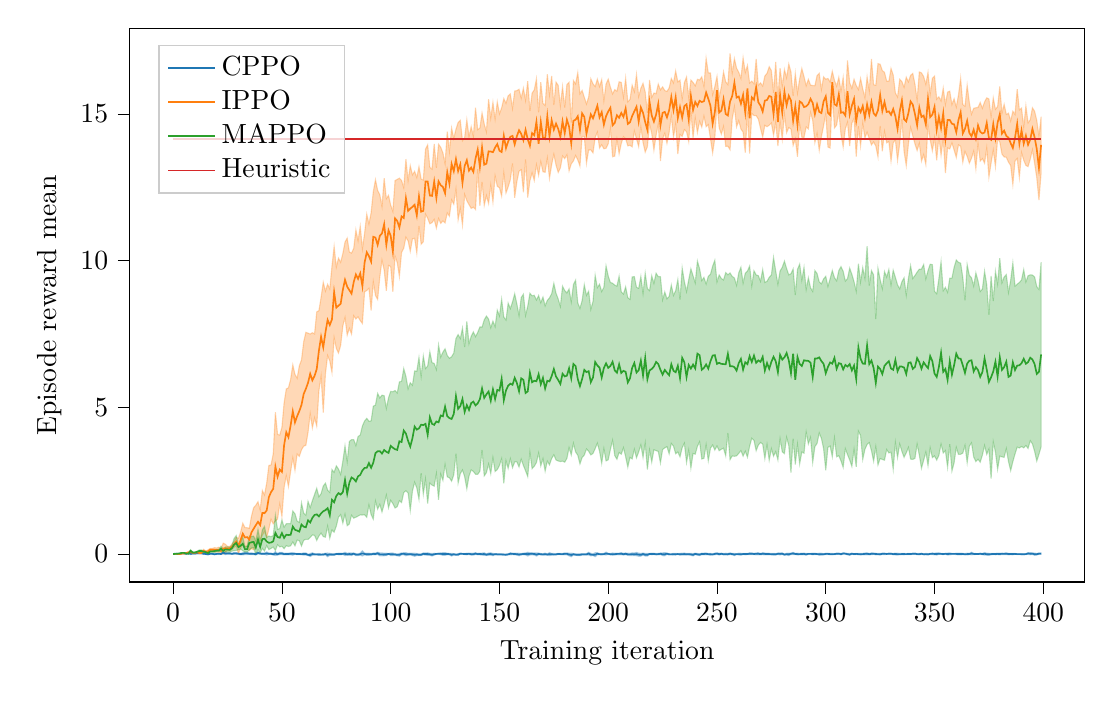
\begin{tikzpicture}

\definecolor{crimson2143940}{RGB}{214,39,40}
\definecolor{darkgray176}{RGB}{176,176,176}
\definecolor{darkorange25512714}{RGB}{255,127,14}
\definecolor{forestgreen4416044}{RGB}{44,160,44}
\definecolor{lightgray204}{RGB}{204,204,204}
\definecolor{steelblue31119180}{RGB}{31,119,180}

\begin{axis}[
scale only axis=true,
width=\linewidth,
height=0.58\linewidth,
legend cell align={left},
legend style={
  fill opacity=0.8,
  draw opacity=1,
  text opacity=1,
  at={(0.03,0.97)},
  anchor=north west,
  draw=lightgray204
},
tick align=outside,
tick pos=left,
x grid style={darkgray176},
xlabel={Training iteration},
xmin=-19.95, xmax=418.95,
xtick style={color=black},
y grid style={darkgray176},
ylabel={Episode reward mean},
ymin=-0.954407606349396, ymax=17.9273464707679,
ytick style={color=black}
]
\path [draw=steelblue31119180, fill=steelblue31119180, opacity=0.3]
(axis cs:0,0)
--(axis cs:0,0)
--(axis cs:1,0.0128932472022884)
--(axis cs:2,0.0130221796743113)
--(axis cs:3,0.0149266710530533)
--(axis cs:4,0.0409082160108726)
--(axis cs:5,0.0409082160108726)
--(axis cs:6,0.0144640357009478)
--(axis cs:7,0.0465341358120476)
--(axis cs:8,0.0315632913276919)
--(axis cs:9,0.0317699261310853)
--(axis cs:10,0.0317699261310853)
--(axis cs:11,0.0428036263751115)
--(axis cs:12,0.0497894334632052)
--(axis cs:13,0.0502873277978372)
--(axis cs:14,0.0229862913207054)
--(axis cs:15,0.0163336967052536)
--(axis cs:16,-0.000883320075110621)
--(axis cs:17,0.0181251249555557)
--(axis cs:18,0.017568308260654)
--(axis cs:19,0.00437522103947526)
--(axis cs:20,0.021753465606346)
--(axis cs:21,0.0272064458140299)
--(axis cs:22,0.0160107958053926)
--(axis cs:23,0.083362677877907)
--(axis cs:24,0.0506083412992606)
--(axis cs:25,0.0374259473390446)
--(axis cs:26,0.038545731999194)
--(axis cs:27,0.0211465385032235)
--(axis cs:28,0.0488582619229396)
--(axis cs:29,0.0481498477247395)
--(axis cs:30,0.0310567290340146)
--(axis cs:31,0.0191429108070148)
--(axis cs:32,0.0440256327359786)
--(axis cs:33,0.0622540965600462)
--(axis cs:34,0.0635175695614092)
--(axis cs:35,0.0289795162963605)
--(axis cs:36,0.0339991514346282)
--(axis cs:37,0.0309900430581349)
--(axis cs:38,0.0274834365082097)
--(axis cs:39,0.0759062795807242)
--(axis cs:40,0.0372259922003013)
--(axis cs:41,0.0264727479821364)
--(axis cs:42,0.0293974362375538)
--(axis cs:43,0.0719018898130538)
--(axis cs:44,0.0282416960778434)
--(axis cs:45,0.0297112127793348)
--(axis cs:46,0.0137579090533906)
--(axis cs:47,0.0842036129859309)
--(axis cs:48,0.0160715107521912)
--(axis cs:49,0.0575662973306797)
--(axis cs:50,0.0565226032228009)
--(axis cs:51,0.0237980832187321)
--(axis cs:52,0.0298629842080967)
--(axis cs:53,0.0309090727026738)
--(axis cs:54,0.0384785578164078)
--(axis cs:55,0.0493371574119012)
--(axis cs:56,0.0242003323574433)
--(axis cs:57,0.0196581256733662)
--(axis cs:58,0.0190911536874986)
--(axis cs:59,0.018621742838895)
--(axis cs:60,0.039732128064349)
--(axis cs:61,0.0397587849943884)
--(axis cs:62,-0.00933253892949602)
--(axis cs:63,0.0192456932492988)
--(axis cs:64,0.0416604660765067)
--(axis cs:65,0.00870013525794525)
--(axis cs:66,0.00584690875363533)
--(axis cs:67,0.016806679353823)
--(axis cs:68,-0.000442896957151238)
--(axis cs:69,0.00128274559961848)
--(axis cs:70,0.0289880259649379)
--(axis cs:71,0.0339520173029856)
--(axis cs:72,0.0218133549786295)
--(axis cs:73,0.00507333194251221)
--(axis cs:74,0.00423927744821016)
--(axis cs:75,0.0177791442193021)
--(axis cs:76,0.0255322683891211)
--(axis cs:77,0.0247383576821539)
--(axis cs:78,0.027593796886405)
--(axis cs:79,0.0587030724051757)
--(axis cs:80,0.0262928344527284)
--(axis cs:81,0.03958254114298)
--(axis cs:82,0.0320938103917305)
--(axis cs:83,0.033971678186227)
--(axis cs:84,0.0133052895591684)
--(axis cs:85,0.00614420170405551)
--(axis cs:86,0.0306178289656753)
--(axis cs:87,0.110978461793109)
--(axis cs:88,0.033829086101223)
--(axis cs:89,0.0251618228089655)
--(axis cs:90,0.0276075974811096)
--(axis cs:91,0.0135319233802663)
--(axis cs:92,0.0333902855176734)
--(axis cs:93,0.0320207922429213)
--(axis cs:94,0.0594518178028522)
--(axis cs:95,0.0406886457339027)
--(axis cs:96,0.0377246631855996)
--(axis cs:97,0.0252228834723549)
--(axis cs:98,0.0270537877318514)
--(axis cs:99,0.0192402680217956)
--(axis cs:100,0.0336615819376362)
--(axis cs:101,0.0328859164489261)
--(axis cs:102,0.0106098421639053)
--(axis cs:103,0.00291242214347083)
--(axis cs:104,0.0185460063430689)
--(axis cs:105,0.0389313572203579)
--(axis cs:106,0.0409735087105113)
--(axis cs:107,0.0469783254407615)
--(axis cs:108,0.0225511869663022)
--(axis cs:109,0.027046853945963)
--(axis cs:110,0.0256516338411937)
--(axis cs:111,0.0249270405473512)
--(axis cs:112,0.0201843712401857)
--(axis cs:113,0.00195037128255196)
--(axis cs:114,-0.000690976044609298)
--(axis cs:115,0.0367982225472354)
--(axis cs:116,0.036297854020321)
--(axis cs:117,0.041123159262478)
--(axis cs:118,0.0227258565689041)
--(axis cs:119,0.0152163337855649)
--(axis cs:120,0.0246134875783477)
--(axis cs:121,0.0167183517990655)
--(axis cs:122,0.0222754803698864)
--(axis cs:123,0.0364257278736762)
--(axis cs:124,0.0442164813436143)
--(axis cs:125,0.0458361645119473)
--(axis cs:126,0.0287196454807819)
--(axis cs:127,0.0206103417124605)
--(axis cs:128,0.0192812784490116)
--(axis cs:129,0.0114196333517521)
--(axis cs:130,-0.00164026172480134)
--(axis cs:131,0.0127881813852865)
--(axis cs:132,0.0307387499478648)
--(axis cs:133,0.014262029362937)
--(axis cs:134,0.0190725746542692)
--(axis cs:135,0.0265756098846001)
--(axis cs:136,0.0270003964417421)
--(axis cs:137,0.0276548265451139)
--(axis cs:138,0.0272896658567563)
--(axis cs:139,0.0432178397699158)
--(axis cs:140,0.0217096226069172)
--(axis cs:141,0.031014745483544)
--(axis cs:142,0.0319062145487561)
--(axis cs:143,0.0426243110752819)
--(axis cs:144,0.00304699526898286)
--(axis cs:145,0.0324838932670963)
--(axis cs:146,0.042063565257703)
--(axis cs:147,0.0188117177104266)
--(axis cs:148,0.00855925315238407)
--(axis cs:149,0.0100224816200893)
--(axis cs:150,0.0121013346841693)
--(axis cs:151,0.00750210078950031)
--(axis cs:152,5.11013055927607e-05)
--(axis cs:153,-0.00239815320889322)
--(axis cs:154,0.00409721730496804)
--(axis cs:155,0.0434668042756848)
--(axis cs:156,0.0311167688951563)
--(axis cs:157,0.0245876951541016)
--(axis cs:158,0.0256977208214343)
--(axis cs:159,0.0249547774869704)
--(axis cs:160,0.0151448053085266)
--(axis cs:161,0.0306268822548407)
--(axis cs:162,0.0364832207375198)
--(axis cs:163,0.0614779030289798)
--(axis cs:164,0.0423516618879692)
--(axis cs:165,0.0426705885963915)
--(axis cs:166,0.0345137082267246)
--(axis cs:167,0.0380048328283198)
--(axis cs:168,0.0332381000262017)
--(axis cs:169,0.0148655049228786)
--(axis cs:170,0.0115896481784017)
--(axis cs:171,0.0310949584331738)
--(axis cs:172,0.00322527660277139)
--(axis cs:173,0.0498214465315383)
--(axis cs:174,0.0172778307838501)
--(axis cs:175,0.0155184731841134)
--(axis cs:176,0.0105819179908524)
--(axis cs:177,0.0222886607489075)
--(axis cs:178,0.018455483442053)
--(axis cs:179,0.0153664104609427)
--(axis cs:180,0.0403172798913231)
--(axis cs:181,0.039136854161899)
--(axis cs:182,0.0275651549757148)
--(axis cs:183,0.0292950058917711)
--(axis cs:184,0.0167023617872142)
--(axis cs:185,0.00298481706261782)
--(axis cs:186,-0.00260713035912077)
--(axis cs:187,0.00484943315044263)
--(axis cs:188,0.0129548794302204)
--(axis cs:189,0.0116527716267506)
--(axis cs:190,0.0120530411930817)
--(axis cs:191,0.0600479156400321)
--(axis cs:192,0.0241002346951211)
--(axis cs:193,0.0030761502066932)
--(axis cs:194,0.0457355444798142)
--(axis cs:195,0.0432894420412924)
--(axis cs:196,0.0156049714052184)
--(axis cs:197,0.0123446371759505)
--(axis cs:198,0.0206019569194901)
--(axis cs:199,0.0636393737371394)
--(axis cs:200,0.0236593311999433)
--(axis cs:201,0.0173029048584275)
--(axis cs:202,0.0352033913101843)
--(axis cs:203,0.0267480163737209)
--(axis cs:204,0.0285720423722979)
--(axis cs:205,0.0320308391225138)
--(axis cs:206,0.0446163113932659)
--(axis cs:207,0.024326782334591)
--(axis cs:208,0.0350500266238069)
--(axis cs:209,0.0252921247864988)
--(axis cs:210,0.0229613265773865)
--(axis cs:211,0.0408225941432813)
--(axis cs:212,0.0360064711426913)
--(axis cs:213,0.0550467857853371)
--(axis cs:214,0.0318479919501663)
--(axis cs:215,0.0184175492412838)
--(axis cs:216,0.0353921672044346)
--(axis cs:217,0.017482188607653)
--(axis cs:218,0.0189308165291069)
--(axis cs:219,0.0224106334549206)
--(axis cs:220,0.0254722298220164)
--(axis cs:221,0.0265504063480492)
--(axis cs:222,0.0137370111483708)
--(axis cs:223,0.0214134043832422)
--(axis cs:224,0.0338313796694416)
--(axis cs:225,0.0373999126125506)
--(axis cs:226,0.0484698491786832)
--(axis cs:227,0.0323319707323037)
--(axis cs:228,0.00849562734119953)
--(axis cs:229,0.00555198968108026)
--(axis cs:230,0.0233182943170177)
--(axis cs:231,0.0234094744496125)
--(axis cs:232,0.0135410660697778)
--(axis cs:233,0.0210431513960997)
--(axis cs:234,0.0294955913521865)
--(axis cs:235,0.0332557495949311)
--(axis cs:236,0.0148374610927739)
--(axis cs:237,0.0204038659361193)
--(axis cs:238,0.0195799905869282)
--(axis cs:239,0.0126989836279841)
--(axis cs:240,0.0295832274767077)
--(axis cs:241,0.0166489941864393)
--(axis cs:242,0.00836243237982096)
--(axis cs:243,0.0278811162697758)
--(axis cs:244,0.0319120068562409)
--(axis cs:245,0.0367964098352161)
--(axis cs:246,0.0157982154289971)
--(axis cs:247,0.0214330482180349)
--(axis cs:248,0.00442611735547379)
--(axis cs:249,0.0311344575886293)
--(axis cs:250,0.0402417204395031)
--(axis cs:251,0.0244614026940098)
--(axis cs:252,0.0285623441169426)
--(axis cs:253,0.0147435027289873)
--(axis cs:254,0.0247353607586295)
--(axis cs:255,0.0204433513032481)
--(axis cs:256,0.0363524314868558)
--(axis cs:257,0.0226179328540933)
--(axis cs:258,0.0207525039987223)
--(axis cs:259,0.0108596332323492)
--(axis cs:260,0.0275324930697813)
--(axis cs:261,0.0238572684929344)
--(axis cs:262,0.0184145778527844)
--(axis cs:263,0.0202178054343617)
--(axis cs:264,0.0178017812616259)
--(axis cs:265,0.0414934513369758)
--(axis cs:266,0.0373141801940155)
--(axis cs:267,0.0226812082213242)
--(axis cs:268,0.0378382988245662)
--(axis cs:269,0.0442999466574248)
--(axis cs:270,0.0197534354517837)
--(axis cs:271,0.043706955937681)
--(axis cs:272,0.0335108131927504)
--(axis cs:273,0.023536558684675)
--(axis cs:274,0.0239633932880242)
--(axis cs:275,0.0150006702723515)
--(axis cs:276,0.020538178700867)
--(axis cs:277,0.0128596226505341)
--(axis cs:278,0.0316257831816577)
--(axis cs:279,0.0383472155610168)
--(axis cs:280,0.0360304610279285)
--(axis cs:281,-0.00186722316636675)
--(axis cs:282,0.0258048778515222)
--(axis cs:283,0.0294372219966755)
--(axis cs:284,0.0317852980676815)
--(axis cs:285,0.0543281929614535)
--(axis cs:286,0.0224684871642792)
--(axis cs:287,0.0261246757605006)
--(axis cs:288,0.0206342297290429)
--(axis cs:289,0.0285289723922144)
--(axis cs:290,0.0329172802764996)
--(axis cs:291,0.0152075870406006)
--(axis cs:292,0.0222602758339614)
--(axis cs:293,0.0230935975809297)
--(axis cs:294,0.0243131157465999)
--(axis cs:295,0.0267493130891335)
--(axis cs:296,0.0156357174273665)
--(axis cs:297,0.025775008129414)
--(axis cs:298,0.025712804903934)
--(axis cs:299,0.00879474120261333)
--(axis cs:300,0.0272139212967701)
--(axis cs:301,0.0254034964365287)
--(axis cs:302,0.0177681047066068)
--(axis cs:303,0.0192726384714805)
--(axis cs:304,0.0113762575612949)
--(axis cs:305,0.0300558846212045)
--(axis cs:306,0.0245001676404357)
--(axis cs:307,0.0180429044649401)
--(axis cs:308,0.037114350891682)
--(axis cs:309,0.0309676903476315)
--(axis cs:310,0.016585662112191)
--(axis cs:311,0.0150858044836428)
--(axis cs:312,0.0283209923739986)
--(axis cs:313,0.0123408074914112)
--(axis cs:314,0.0218490499604553)
--(axis cs:315,0.0208673395147042)
--(axis cs:316,0.0165347183563513)
--(axis cs:317,0.0209748967732763)
--(axis cs:318,0.0332434743234421)
--(axis cs:319,0.0384176523576967)
--(axis cs:320,0.0192494134118056)
--(axis cs:321,0.0354548712554727)
--(axis cs:322,0.0308343121964261)
--(axis cs:323,0.0252651647355971)
--(axis cs:324,0.0164978362988715)
--(axis cs:325,0.0155071270894087)
--(axis cs:326,0.0281164465305384)
--(axis cs:327,0.0299687990223284)
--(axis cs:328,0.0165801043985706)
--(axis cs:329,0.0263956795915637)
--(axis cs:330,0.0253546017969768)
--(axis cs:331,0.0184307870941843)
--(axis cs:332,0.0312813739585175)
--(axis cs:333,0.0278977381420004)
--(axis cs:334,0.0154894730084918)
--(axis cs:335,0.0180115009597707)
--(axis cs:336,0.0227639704635991)
--(axis cs:337,0.00784165506362156)
--(axis cs:338,0.0230730435486031)
--(axis cs:339,0.0178542446863701)
--(axis cs:340,0.0244914860984917)
--(axis cs:341,0.0302428062292755)
--(axis cs:342,0.0136974116191557)
--(axis cs:343,0.0186691507219295)
--(axis cs:344,0.0259232795376895)
--(axis cs:345,0.00436507351622024)
--(axis cs:346,0.0220265082507278)
--(axis cs:347,0.0111102428374933)
--(axis cs:348,0.0210922507548516)
--(axis cs:349,0.03491827272697)
--(axis cs:350,0.0292015885782948)
--(axis cs:351,0.0361450284499012)
--(axis cs:352,0.0336815640085269)
--(axis cs:353,0.0208498374810281)
--(axis cs:354,0.0140147166699968)
--(axis cs:355,0.0202958334412035)
--(axis cs:356,0.0310739202000265)
--(axis cs:357,0.039085528639257)
--(axis cs:358,0.0212992167455853)
--(axis cs:359,0.0195556031892744)
--(axis cs:360,0.0267659969441301)
--(axis cs:361,0.0261688121056698)
--(axis cs:362,0.0282408988227503)
--(axis cs:363,0.0219831320830837)
--(axis cs:364,0.0133996456869703)
--(axis cs:365,0.0278433976626692)
--(axis cs:366,0.0209807029082396)
--(axis cs:367,0.0613586171138193)
--(axis cs:368,0.0245004146165232)
--(axis cs:369,0.0147263240827673)
--(axis cs:370,0.00940279428546794)
--(axis cs:371,0.0289713553977544)
--(axis cs:372,0.0190098281216064)
--(axis cs:373,0.0487783460577976)
--(axis cs:374,0.0287697075310348)
--(axis cs:375,0.0228533377647756)
--(axis cs:376,0.0222431600787177)
--(axis cs:377,0.0172072316436001)
--(axis cs:378,0.0221136933087176)
--(axis cs:379,0.0275511801620204)
--(axis cs:380,0.0297234845827138)
--(axis cs:381,0.0312322033849316)
--(axis cs:382,0.0289092089497644)
--(axis cs:383,0.0397852329431359)
--(axis cs:384,0.0219059761137107)
--(axis cs:385,0.0204457020197769)
--(axis cs:386,0.021429472224773)
--(axis cs:387,0.0169756085446295)
--(axis cs:388,0.00904402618406267)
--(axis cs:389,0.0147002434274045)
--(axis cs:390,0.00740175508506535)
--(axis cs:391,0.00497336171362533)
--(axis cs:392,0.0110448509014156)
--(axis cs:393,0.0473616295094444)
--(axis cs:394,0.0444866073908962)
--(axis cs:395,0.039985844601752)
--(axis cs:396,0.0299335825052954)
--(axis cs:397,0.0185751120548916)
--(axis cs:398,0.0353203992890911)
--(axis cs:399,0.0335556059844186)
--(axis cs:399,-0.00995999525986345)
--(axis cs:399,-0.00995999525986345)
--(axis cs:398,-0.0123279176839735)
--(axis cs:397,-0.0334195995630296)
--(axis cs:396,-0.0444331117616105)
--(axis cs:395,-0.0160360623264788)
--(axis cs:394,-0.0254162109675564)
--(axis cs:393,-0.0127990093683239)
--(axis cs:392,-0.0165216092646566)
--(axis cs:391,-0.0235114171335472)
--(axis cs:390,-0.0231403905973707)
--(axis cs:389,-0.022277151962832)
--(axis cs:388,-0.0189148193089489)
--(axis cs:387,-0.0101948473778892)
--(axis cs:386,-0.0259257244966372)
--(axis cs:385,-0.0225359652871787)
--(axis cs:384,-0.0286639002572271)
--(axis cs:383,-0.0163381877228668)
--(axis cs:382,-0.0213323534948607)
--(axis cs:381,-0.0186101500266417)
--(axis cs:380,-0.0283965744770284)
--(axis cs:379,-0.020996058972922)
--(axis cs:378,-0.0251090614185267)
--(axis cs:377,-0.0157449350565519)
--(axis cs:376,-0.029479560366342)
--(axis cs:375,-0.045150802771286)
--(axis cs:374,-0.0413995311887942)
--(axis cs:373,-0.0377283972595121)
--(axis cs:372,-0.0238104480295468)
--(axis cs:371,-0.0134524411740594)
--(axis cs:370,-0.0121317524153508)
--(axis cs:369,-0.0144593459043105)
--(axis cs:368,-0.0203401015684885)
--(axis cs:367,-0.0274215485984655)
--(axis cs:366,-0.0205306243053257)
--(axis cs:365,-0.0331629633297156)
--(axis cs:364,-0.027230364340977)
--(axis cs:363,-0.0222734090507254)
--(axis cs:362,-0.0261556835720992)
--(axis cs:361,-0.0273398695510533)
--(axis cs:360,-0.0211167740866373)
--(axis cs:359,-0.0103018215527184)
--(axis cs:358,-0.0146275714051133)
--(axis cs:357,-0.0299605566137036)
--(axis cs:356,-0.0351412319082868)
--(axis cs:355,-0.0066757810808275)
--(axis cs:354,-0.0183850288309126)
--(axis cs:353,-0.0123450678218959)
--(axis cs:352,-0.0110497155864058)
--(axis cs:351,-0.0363136168762792)
--(axis cs:350,-0.025608594997993)
--(axis cs:349,-0.0220446188912495)
--(axis cs:348,-0.013329570868921)
--(axis cs:347,-0.0324455326907862)
--(axis cs:346,-0.0313601526938159)
--(axis cs:345,-0.0210142987467988)
--(axis cs:344,-0.0141636397565049)
--(axis cs:343,-0.0287153678985788)
--(axis cs:342,-0.0226059322474746)
--(axis cs:341,-0.00680644639990263)
--(axis cs:340,-0.00771083559266955)
--(axis cs:339,-0.0205145171308604)
--(axis cs:338,-0.0224790739915827)
--(axis cs:337,-0.0169439316164695)
--(axis cs:336,-0.0263895994604631)
--(axis cs:335,-0.0225819448548987)
--(axis cs:334,-0.0269768702871893)
--(axis cs:333,-0.0381240429380073)
--(axis cs:332,-0.0321534350990407)
--(axis cs:331,-0.0263247874629337)
--(axis cs:330,-0.00707799725053578)
--(axis cs:329,-0.006744797057719)
--(axis cs:328,-0.01433512064701)
--(axis cs:327,-0.0172808870350237)
--(axis cs:326,-0.0146111827092354)
--(axis cs:325,-0.0331470544236644)
--(axis cs:324,-0.0257866512864438)
--(axis cs:323,-0.0278567900024751)
--(axis cs:322,-0.0122516417727065)
--(axis cs:321,-0.0213841020915992)
--(axis cs:320,-0.0311696503439701)
--(axis cs:319,-0.0245411485192635)
--(axis cs:318,-0.0241092985978698)
--(axis cs:317,-0.0305450609239382)
--(axis cs:316,-0.0310760239638273)
--(axis cs:315,-0.028588957611257)
--(axis cs:314,-0.0142122210080898)
--(axis cs:313,-0.0195392998270874)
--(axis cs:312,-0.0111504592724545)
--(axis cs:311,-0.0467209490352378)
--(axis cs:310,-0.0260530868277369)
--(axis cs:309,-0.00712410734660067)
--(axis cs:308,-0.000968831274586943)
--(axis cs:307,-0.0290490238179295)
--(axis cs:306,-0.00429851850442223)
--(axis cs:305,-0.0140500635571314)
--(axis cs:304,-0.0176829829298517)
--(axis cs:303,-0.0286766005008317)
--(axis cs:302,-0.0261544665973285)
--(axis cs:301,-0.0195037068382756)
--(axis cs:300,-0.0178312169735857)
--(axis cs:299,-0.0281925971860798)
--(axis cs:298,-0.0366029984192877)
--(axis cs:297,-0.0420527134777466)
--(axis cs:296,-0.0206839630072504)
--(axis cs:295,-0.0187835682228684)
--(axis cs:294,-0.0259058550668666)
--(axis cs:293,-0.0124988523687986)
--(axis cs:292,-0.011825434870318)
--(axis cs:291,-0.0395200921720162)
--(axis cs:290,-0.0275790607398242)
--(axis cs:289,-0.023605391554889)
--(axis cs:288,-0.0321071485658578)
--(axis cs:287,-0.0330491057599581)
--(axis cs:286,-0.0189493733085865)
--(axis cs:285,-0.017535115704509)
--(axis cs:284,-0.0153800889183722)
--(axis cs:283,-0.0539924664890823)
--(axis cs:282,-0.0342390378721385)
--(axis cs:281,-0.0411813888073945)
--(axis cs:280,-0.013776586096725)
--(axis cs:279,-0.0329773594683518)
--(axis cs:278,-0.0147229816357726)
--(axis cs:277,-0.0343843529090519)
--(axis cs:276,-0.03412276638959)
--(axis cs:275,-0.0292426410060638)
--(axis cs:274,-0.0279743821592807)
--(axis cs:273,-0.0238905199012709)
--(axis cs:272,-0.0283115647381282)
--(axis cs:271,-0.0223601855451571)
--(axis cs:270,-0.0273429071782186)
--(axis cs:269,-0.029471616511483)
--(axis cs:268,-0.0284926935446561)
--(axis cs:267,-0.0210735153856255)
--(axis cs:266,-0.0203742498080021)
--(axis cs:265,-0.0219974494067636)
--(axis cs:264,-0.0231820268646059)
--(axis cs:263,-0.025004267158537)
--(axis cs:262,-0.0216338971071252)
--(axis cs:261,-0.0402860506381167)
--(axis cs:260,-0.0355285201798424)
--(axis cs:259,-0.01958247959761)
--(axis cs:258,-0.0567066360788004)
--(axis cs:257,-0.0275147782850109)
--(axis cs:256,-0.0192303184812512)
--(axis cs:255,-0.0339895616982134)
--(axis cs:254,-0.0339311246000665)
--(axis cs:253,-0.0292647285522837)
--(axis cs:252,-0.0156206749949786)
--(axis cs:251,-0.0373324411798475)
--(axis cs:250,-0.0116607835837631)
--(axis cs:249,-0.0270237732091855)
--(axis cs:248,-0.0332411603640361)
--(axis cs:247,-0.0415820799630979)
--(axis cs:246,-0.0269751651758777)
--(axis cs:245,-0.0273589801951879)
--(axis cs:244,-0.0289900400322379)
--(axis cs:243,-0.0243563987614162)
--(axis cs:242,-0.0542315772433735)
--(axis cs:241,-0.0407934172772636)
--(axis cs:240,-0.0217884354463837)
--(axis cs:239,-0.0662911611250002)
--(axis cs:238,-0.0456296635467112)
--(axis cs:237,-0.03190733561521)
--(axis cs:236,-0.0319728584457438)
--(axis cs:235,-0.0379954778341957)
--(axis cs:234,-0.0376607728300511)
--(axis cs:233,-0.0400224482172807)
--(axis cs:232,-0.0172705441039002)
--(axis cs:231,-0.0358349818891199)
--(axis cs:230,-0.0342147399539538)
--(axis cs:229,-0.0306682277453164)
--(axis cs:228,-0.0305910640975525)
--(axis cs:227,-0.0147742275197896)
--(axis cs:226,-0.0634091361524245)
--(axis cs:225,-0.0567139600478694)
--(axis cs:224,-0.0193633949722052)
--(axis cs:223,-0.0299747633649045)
--(axis cs:222,-0.030997664770638)
--(axis cs:221,-0.0210246902022159)
--(axis cs:220,-0.0250281685913972)
--(axis cs:219,-0.0193192441271237)
--(axis cs:218,-0.0727925702047796)
--(axis cs:217,-0.070077457941135)
--(axis cs:216,-0.0368459458553602)
--(axis cs:215,-0.0751274830520477)
--(axis cs:214,-0.0773250010888097)
--(axis cs:213,-0.0598585940535663)
--(axis cs:212,-0.0541504574937712)
--(axis cs:211,-0.0499488782770263)
--(axis cs:210,-0.0510841013373149)
--(axis cs:209,-0.0485621570753898)
--(axis cs:208,-0.0224120827061057)
--(axis cs:207,-0.0376514012039487)
--(axis cs:206,-0.0249969287216525)
--(axis cs:205,-0.0250471626359687)
--(axis cs:204,-0.023538025904939)
--(axis cs:203,-0.0371340836786573)
--(axis cs:202,-0.0428533428211435)
--(axis cs:201,-0.031015138850945)
--(axis cs:200,-0.0142093944434826)
--(axis cs:199,-0.0341104464639189)
--(axis cs:198,-0.0272495423082673)
--(axis cs:197,-0.0278475202393728)
--(axis cs:196,-0.0257598082646881)
--(axis cs:195,-0.0275712439258792)
--(axis cs:194,-0.0938087154596319)
--(axis cs:193,-0.0505195203224793)
--(axis cs:192,-0.0646551849649824)
--(axis cs:191,-0.0353287324599649)
--(axis cs:190,-0.0359756234511708)
--(axis cs:189,-0.0396117644788556)
--(axis cs:188,-0.0370612333825563)
--(axis cs:187,-0.0560831890829842)
--(axis cs:186,-0.0512783846419643)
--(axis cs:185,-0.0473668616456833)
--(axis cs:184,-0.0337666481445844)
--(axis cs:183,-0.0959434891681383)
--(axis cs:182,-0.0620716957176591)
--(axis cs:181,-0.0291040138569945)
--(axis cs:180,-0.0297949682066373)
--(axis cs:179,-0.0256187219045344)
--(axis cs:178,-0.024080114687984)
--(axis cs:177,-0.0173951469828092)
--(axis cs:176,-0.0348547960835511)
--(axis cs:175,-0.0413446264094824)
--(axis cs:174,-0.0381616141795307)
--(axis cs:173,-0.0553007208574389)
--(axis cs:172,-0.0387247501230356)
--(axis cs:171,-0.0388624944169726)
--(axis cs:170,-0.0408653261772623)
--(axis cs:169,-0.0316523935115467)
--(axis cs:168,-0.0313968230853504)
--(axis cs:167,-0.071154051917404)
--(axis cs:166,-0.0341257693999429)
--(axis cs:165,-0.0317302530047574)
--(axis cs:164,-0.0341959551559059)
--(axis cs:163,-0.0692587579824232)
--(axis cs:162,-0.0341534961077997)
--(axis cs:161,-0.0274790296755275)
--(axis cs:160,-0.033399583972771)
--(axis cs:159,-0.0596875240350932)
--(axis cs:158,-0.0397577653803655)
--(axis cs:157,-0.0255037777482314)
--(axis cs:156,-0.022802419644917)
--(axis cs:155,-0.0301568133489199)
--(axis cs:154,-0.029290817429751)
--(axis cs:153,-0.0454234642910925)
--(axis cs:152,-0.0407458413948789)
--(axis cs:151,-0.0354666715767182)
--(axis cs:150,-0.0382956426628301)
--(axis cs:149,-0.0347189376815585)
--(axis cs:148,-0.0246863182144821)
--(axis cs:147,-0.0573567663234738)
--(axis cs:146,-0.0416903479928918)
--(axis cs:145,-0.0427697200943544)
--(axis cs:144,-0.0504907630245027)
--(axis cs:143,-0.0462460524761066)
--(axis cs:142,-0.0397398704606127)
--(axis cs:141,-0.0318083593412371)
--(axis cs:140,-0.0298155065746316)
--(axis cs:139,-0.0148920823547243)
--(axis cs:138,-0.038919474070732)
--(axis cs:137,-0.0401611916920534)
--(axis cs:136,-0.0140841310859437)
--(axis cs:135,-0.0276030350148085)
--(axis cs:134,-0.0212853353472813)
--(axis cs:133,-0.00502974566474903)
--(axis cs:132,-0.00605065244504751)
--(axis cs:131,-0.0511681057309376)
--(axis cs:130,-0.0449421594720303)
--(axis cs:129,-0.0308905331873636)
--(axis cs:128,-0.0720684222001955)
--(axis cs:127,-0.0291823521765989)
--(axis cs:126,-0.0251934153035366)
--(axis cs:125,-0.0453126566519755)
--(axis cs:124,-0.0465872536029361)
--(axis cs:123,-0.0255493082608549)
--(axis cs:122,-0.00506908490276398)
--(axis cs:121,-0.0111664063875806)
--(axis cs:120,-0.0398105995148984)
--(axis cs:119,-0.0714567716110858)
--(axis cs:118,-0.045752962896817)
--(axis cs:117,-0.0444480070136715)
--(axis cs:116,-0.0388522940750177)
--(axis cs:115,-0.0260583654271841)
--(axis cs:114,-0.0494183531790235)
--(axis cs:113,-0.0541271375410091)
--(axis cs:112,-0.0545897131482226)
--(axis cs:111,-0.0790209948455826)
--(axis cs:110,-0.0563261474425089)
--(axis cs:109,-0.0356969978872065)
--(axis cs:108,-0.041575078728865)
--(axis cs:107,-0.0594036516220666)
--(axis cs:106,-0.0286644978869436)
--(axis cs:105,-0.0308382566190284)
--(axis cs:104,-0.0768045872330484)
--(axis cs:103,-0.0619624396063072)
--(axis cs:102,-0.0403796671803097)
--(axis cs:101,-0.0532559717535594)
--(axis cs:100,-0.0556117392820235)
--(axis cs:99,-0.0138099842407398)
--(axis cs:98,-0.0558064834512524)
--(axis cs:97,-0.0587820388777536)
--(axis cs:96,-0.0650274988179977)
--(axis cs:95,-0.0641998795934947)
--(axis cs:94,-0.0153248082823948)
--(axis cs:93,-0.0308581954343818)
--(axis cs:92,-0.0263730883824282)
--(axis cs:91,-0.0356129373621094)
--(axis cs:90,-0.0430091664237094)
--(axis cs:89,-0.0485627714589621)
--(axis cs:88,-0.0305617925478756)
--(axis cs:87,-0.0693663156274736)
--(axis cs:86,-0.0407395651836576)
--(axis cs:85,-0.0517494966734023)
--(axis cs:84,-0.0542206857762366)
--(axis cs:83,-0.0160755130052896)
--(axis cs:82,-0.0516947125252483)
--(axis cs:81,-0.0425315908223506)
--(axis cs:80,-0.043913295031397)
--(axis cs:79,-0.0534926748967664)
--(axis cs:78,-0.0181588706965547)
--(axis cs:77,-0.0281541647703701)
--(axis cs:76,-0.0249180114397615)
--(axis cs:75,-0.0174296823815939)
--(axis cs:74,-0.0440959677490457)
--(axis cs:73,-0.0430169621055351)
--(axis cs:72,-0.0467636493793325)
--(axis cs:71,-0.0961460573895199)
--(axis cs:70,-0.0311671553824381)
--(axis cs:69,-0.0383804349103281)
--(axis cs:68,-0.0416248440701981)
--(axis cs:67,-0.0498944521216584)
--(axis cs:66,-0.0322483437579756)
--(axis cs:65,-0.0336488542770988)
--(axis cs:64,-0.0436209627000667)
--(axis cs:63,-0.0881698892806573)
--(axis cs:62,-0.051619549689381)
--(axis cs:61,-0.0368962488819209)
--(axis cs:60,-0.0366521674156182)
--(axis cs:59,-0.0294931298967291)
--(axis cs:58,-0.0187431049475355)
--(axis cs:57,-0.0235521914304601)
--(axis cs:56,-0.0100879268083447)
--(axis cs:55,-0.0431048167629804)
--(axis cs:54,-0.0248292465118513)
--(axis cs:53,-0.0299887473174742)
--(axis cs:52,-0.0302270373712137)
--(axis cs:51,-0.0322115671520321)
--(axis cs:50,-0.0200371261991464)
--(axis cs:49,-0.0202258292404812)
--(axis cs:48,-0.0359875090170101)
--(axis cs:47,-0.0508063033837243)
--(axis cs:46,-0.0320304259462496)
--(axis cs:45,-0.0142988694362359)
--(axis cs:44,-0.0127642273542072)
--(axis cs:43,-0.0372253570354413)
--(axis cs:42,-0.0119644519914058)
--(axis cs:41,-0.0121981272229663)
--(axis cs:40,-0.00914047424676767)
--(axis cs:39,-0.00328103744480723)
--(axis cs:38,-0.0331045211348303)
--(axis cs:37,-0.0224839166543263)
--(axis cs:36,-0.0226166201107535)
--(axis cs:35,-0.0136893910333376)
--(axis cs:34,-0.0184273223012096)
--(axis cs:33,-0.0185870394373621)
--(axis cs:32,-0.0312681386665946)
--(axis cs:31,-0.026631064141912)
--(axis cs:30,-0.0131891302942888)
--(axis cs:29,-0.00811439223293176)
--(axis cs:28,-0.00854773707771151)
--(axis cs:27,-0.0115017669658281)
--(axis cs:26,-0.000779911178067725)
--(axis cs:25,0.00081468344946423)
--(axis cs:24,-0.018159396077183)
--(axis cs:23,0.00245571879635512)
--(axis cs:22,-0.0151342973957317)
--(axis cs:21,-0.015478938964529)
--(axis cs:20,-0.0147832045238413)
--(axis cs:19,-0.0244376024252133)
--(axis cs:18,-0.00478644875680203)
--(axis cs:17,-0.00469391756252362)
--(axis cs:16,-0.0260811400253358)
--(axis cs:15,-0.0149379546067632)
--(axis cs:14,-0.00915243511268332)
--(axis cs:13,0.00239595992867102)
--(axis cs:12,0.00237223755313962)
--(axis cs:11,0.00270173939967061)
--(axis cs:10,0.000351469403853933)
--(axis cs:9,0.000351469403853933)
--(axis cs:8,-0.0205742801989484)
--(axis cs:7,0.00660948930691785)
--(axis cs:6,-0.00578961949207972)
--(axis cs:5,0.00866984456312916)
--(axis cs:4,0.00866984456312916)
--(axis cs:3,0.00128771465926735)
--(axis cs:2,0.0109786451480085)
--(axis cs:1,0.0108699456910976)
--(axis cs:0,0)
--cycle;

\path [draw=darkorange25512714, fill=darkorange25512714, opacity=0.3]
(axis cs:0,0)
--(axis cs:0,0)
--(axis cs:1,0.00552014744083999)
--(axis cs:2,0.00325923843231999)
--(axis cs:3,0.0021651936602185)
--(axis cs:4,0.018139693386344)
--(axis cs:5,0.0177768995186172)
--(axis cs:6,0.0430331254397652)
--(axis cs:7,0.0787927540150514)
--(axis cs:8,0.118324440663549)
--(axis cs:9,0.0546784723594703)
--(axis cs:10,0.0546784723594703)
--(axis cs:11,0.0837730391562255)
--(axis cs:12,0.0516193050521626)
--(axis cs:13,0.0629778541504333)
--(axis cs:14,0.159807464212026)
--(axis cs:15,0.10237404021782)
--(axis cs:16,0.138230702396087)
--(axis cs:17,0.187960601657793)
--(axis cs:18,0.188641326777009)
--(axis cs:19,0.216595040881952)
--(axis cs:20,0.204329834484823)
--(axis cs:21,0.233246454974198)
--(axis cs:22,0.170550734081085)
--(axis cs:23,0.36892994699559)
--(axis cs:24,0.332935171672832)
--(axis cs:25,0.258773633330215)
--(axis cs:26,0.259427454175547)
--(axis cs:27,0.336617657315928)
--(axis cs:28,0.427121763760881)
--(axis cs:29,0.570371877490825)
--(axis cs:30,0.533900297207922)
--(axis cs:31,0.743770150621877)
--(axis cs:32,1.04966373368919)
--(axis cs:33,0.902812442294423)
--(axis cs:34,0.894309727297698)
--(axis cs:35,0.875457874437078)
--(axis cs:36,1.28768722656032)
--(axis cs:37,1.57947713254472)
--(axis cs:38,1.6633521673056)
--(axis cs:39,1.784111164361)
--(axis cs:40,1.50403756549702)
--(axis cs:41,2.1672347323919)
--(axis cs:42,2.01729368991094)
--(axis cs:43,2.41932685848373)
--(axis cs:44,3.0207386267321)
--(axis cs:45,3.03565564661853)
--(axis cs:46,3.41293904786959)
--(axis cs:47,4.83330864543234)
--(axis cs:48,4.07474050613758)
--(axis cs:49,4.05512990931425)
--(axis cs:50,4.32225347353368)
--(axis cs:51,5.15343760662043)
--(axis cs:52,5.62766209740387)
--(axis cs:53,5.6679963489213)
--(axis cs:54,5.95460323427573)
--(axis cs:55,6.45221982502737)
--(axis cs:56,6.12398744889725)
--(axis cs:57,5.99199967102013)
--(axis cs:58,6.4187180333424)
--(axis cs:59,6.61718058388413)
--(axis cs:60,7.23346069481439)
--(axis cs:61,7.55792483155469)
--(axis cs:62,7.53009883277564)
--(axis cs:63,7.49976610241232)
--(axis cs:64,7.54554084027681)
--(axis cs:65,7.50225133396533)
--(axis cs:66,8.25412963155998)
--(axis cs:67,8.2972636727619)
--(axis cs:68,8.75048550712501)
--(axis cs:69,9.26727175446124)
--(axis cs:70,8.96309051251688)
--(axis cs:71,9.19702032856857)
--(axis cs:72,9.03506983101762)
--(axis cs:73,9.80912118465035)
--(axis cs:74,10.4872169313336)
--(axis cs:75,9.78398125802894)
--(axis cs:76,10.0879016017631)
--(axis cs:77,9.94668954736291)
--(axis cs:78,10.2441186854373)
--(axis cs:79,10.6361560065892)
--(axis cs:80,10.7707278256172)
--(axis cs:81,10.2958008224063)
--(axis cs:82,10.261379318983)
--(axis cs:83,10.417408247321)
--(axis cs:84,11.0519673730834)
--(axis cs:85,10.6767625547631)
--(axis cs:86,11.1793149236152)
--(axis cs:87,10.4076621484329)
--(axis cs:88,10.9347791149624)
--(axis cs:89,11.5888434139418)
--(axis cs:90,11.2530678988953)
--(axis cs:91,11.634340678628)
--(axis cs:92,12.3530368007719)
--(axis cs:93,12.7633797621951)
--(axis cs:94,12.3998717483433)
--(axis cs:95,12.2471296824868)
--(axis cs:96,11.8493146499417)
--(axis cs:97,12.813223083807)
--(axis cs:98,12.1145763258483)
--(axis cs:99,12.2306633149731)
--(axis cs:100,11.8959275892985)
--(axis cs:101,11.6798983693298)
--(axis cs:102,12.7305860983273)
--(axis cs:103,12.7735954029184)
--(axis cs:104,12.814539495088)
--(axis cs:105,12.7390401202079)
--(axis cs:106,12.4881576554193)
--(axis cs:107,13.4664740623607)
--(axis cs:108,12.7242727605411)
--(axis cs:109,13.2415622966847)
--(axis cs:110,12.9254140759052)
--(axis cs:111,13.0487035514765)
--(axis cs:112,12.834364074548)
--(axis cs:113,13.2062804091252)
--(axis cs:114,12.7815750862216)
--(axis cs:115,12.7528313792383)
--(axis cs:116,13.8080158209609)
--(axis cs:117,13.9516374802515)
--(axis cs:118,13.1869217232079)
--(axis cs:119,13.1217804157101)
--(axis cs:120,13.9853370189586)
--(axis cs:121,13.1713281665384)
--(axis cs:122,13.9724262986493)
--(axis cs:123,13.8691835749659)
--(axis cs:124,13.6791508946821)
--(axis cs:125,13.3059820753239)
--(axis cs:126,14.403194381469)
--(axis cs:127,13.7304816847239)
--(axis cs:128,14.5256440626846)
--(axis cs:129,14.1740689269466)
--(axis cs:130,14.4804803125591)
--(axis cs:131,14.714118892933)
--(axis cs:132,14.7835034781494)
--(axis cs:133,14.0920680931696)
--(axis cs:134,14.2004136916003)
--(axis cs:135,14.8047285171776)
--(axis cs:136,14.229935171861)
--(axis cs:137,14.5711249727826)
--(axis cs:138,14.2337024415418)
--(axis cs:139,15.2193619882029)
--(axis cs:140,14.4696568773335)
--(axis cs:141,14.5198392103365)
--(axis cs:142,15.0381458274055)
--(axis cs:143,14.6619606863976)
--(axis cs:144,14.3977379703514)
--(axis cs:145,15.510698766601)
--(axis cs:146,14.8662394432508)
--(axis cs:147,15.4038435160915)
--(axis cs:148,14.8272808145202)
--(axis cs:149,15.415875111907)
--(axis cs:150,15.0117310852268)
--(axis cs:151,15.2112349754852)
--(axis cs:152,15.529395229643)
--(axis cs:153,15.3682323064139)
--(axis cs:154,15.6226572916145)
--(axis cs:155,15.6867286170247)
--(axis cs:156,15.1971995881935)
--(axis cs:157,15.7847947366458)
--(axis cs:158,15.7992766616603)
--(axis cs:159,15.8461533338131)
--(axis cs:160,15.5436352016978)
--(axis cs:161,15.8825647741723)
--(axis cs:162,15.4659827611569)
--(axis cs:163,16.1240801295725)
--(axis cs:164,15.1056479546233)
--(axis cs:165,15.7121903642967)
--(axis cs:166,15.8264672196641)
--(axis cs:167,16.2010743809648)
--(axis cs:168,15.0566971323392)
--(axis cs:169,16.089167160667)
--(axis cs:170,15.3658048331606)
--(axis cs:171,15.2927314416543)
--(axis cs:172,16.356402872686)
--(axis cs:173,15.6642614209296)
--(axis cs:174,16.3027855967978)
--(axis cs:175,15.3085478910743)
--(axis cs:176,16.0898388237425)
--(axis cs:177,15.9813245305566)
--(axis cs:178,15.2789637383561)
--(axis cs:179,15.9344083686362)
--(axis cs:180,15.2219587455773)
--(axis cs:181,16.0080526924151)
--(axis cs:182,16.0814023768705)
--(axis cs:183,14.7102643802339)
--(axis cs:184,16.1448888414506)
--(axis cs:185,16.0255484683464)
--(axis cs:186,16.4153918471654)
--(axis cs:187,15.6891542301994)
--(axis cs:188,15.8072321101493)
--(axis cs:189,15.5728919004931)
--(axis cs:190,15.3435348925479)
--(axis cs:191,15.5764825803385)
--(axis cs:192,16.2041381451927)
--(axis cs:193,16.0317377853587)
--(axis cs:194,15.9389619287803)
--(axis cs:195,16.1908632328324)
--(axis cs:196,15.937444308827)
--(axis cs:197,16.1755908675318)
--(axis cs:198,15.4592942422902)
--(axis cs:199,16.0231156776026)
--(axis cs:200,16.1907774989549)
--(axis cs:201,15.9201728859957)
--(axis cs:202,15.6882746746436)
--(axis cs:203,15.8347833061678)
--(axis cs:204,15.7802423126805)
--(axis cs:205,16.1009459292564)
--(axis cs:206,16.0791860933854)
--(axis cs:207,15.5824428592633)
--(axis cs:208,16.2252880491296)
--(axis cs:209,15.4134656911008)
--(axis cs:210,15.4997673627204)
--(axis cs:211,15.9867184867058)
--(axis cs:212,15.7627608782133)
--(axis cs:213,16.3473397205068)
--(axis cs:214,15.5963946683714)
--(axis cs:215,15.8790220783604)
--(axis cs:216,16.049206689578)
--(axis cs:217,15.7533955565304)
--(axis cs:218,15.0392943895823)
--(axis cs:219,16.1620965933167)
--(axis cs:220,15.5695927816129)
--(axis cs:221,15.7170314541703)
--(axis cs:222,15.6930570842145)
--(axis cs:223,16.0231712979578)
--(axis cs:224,15.8237406807278)
--(axis cs:225,15.9273773885238)
--(axis cs:226,15.8005214673105)
--(axis cs:227,15.7727674488319)
--(axis cs:228,15.8887006535716)
--(axis cs:229,16.2169926363196)
--(axis cs:230,16.0668414650443)
--(axis cs:231,16.47124359785)
--(axis cs:232,16.0947769500983)
--(axis cs:233,16.1536556789897)
--(axis cs:234,15.5208062064019)
--(axis cs:235,16.0764267694809)
--(axis cs:236,16.2645670923611)
--(axis cs:237,15.5688500429052)
--(axis cs:238,16.1589157964359)
--(axis cs:239,16.0803955302647)
--(axis cs:240,15.9644203455124)
--(axis cs:241,16.1868696764138)
--(axis cs:242,16.1601535944893)
--(axis cs:243,16.2705670684739)
--(axis cs:244,15.9474796618873)
--(axis cs:245,16.903494075524)
--(axis cs:246,16.4027355412985)
--(axis cs:247,16.4014318055848)
--(axis cs:248,15.6628700781375)
--(axis cs:249,15.9390262465249)
--(axis cs:250,16.284295580693)
--(axis cs:251,15.5801911228479)
--(axis cs:252,15.9230732550756)
--(axis cs:253,16.4427146367255)
--(axis cs:254,16.1011579898362)
--(axis cs:255,16.0049576878839)
--(axis cs:256,17.069084921808)
--(axis cs:257,16.399638430446)
--(axis cs:258,16.88919517937)
--(axis cs:259,16.5645755118138)
--(axis cs:260,16.4245579008216)
--(axis cs:261,16.2169142108476)
--(axis cs:262,16.9185521847083)
--(axis cs:263,16.4170467094666)
--(axis cs:264,16.657997524513)
--(axis cs:265,16.0573487692504)
--(axis cs:266,16.1230083397957)
--(axis cs:267,16.0296266523955)
--(axis cs:268,16.8832710847479)
--(axis cs:269,15.9790918198808)
--(axis cs:270,16.0638652070847)
--(axis cs:271,15.9538548799463)
--(axis cs:272,16.2988649243371)
--(axis cs:273,16.390681695671)
--(axis cs:274,16.6166446479202)
--(axis cs:275,16.4817139575896)
--(axis cs:276,15.7270321561592)
--(axis cs:277,16.7775794478799)
--(axis cs:278,15.5464286703223)
--(axis cs:279,16.5677664380987)
--(axis cs:280,15.9509999341681)
--(axis cs:281,16.5171453206903)
--(axis cs:282,16.2382269707005)
--(axis cs:283,16.709779650166)
--(axis cs:284,16.4347822816519)
--(axis cs:285,15.6152979376238)
--(axis cs:286,16.3872617036901)
--(axis cs:287,15.7186621933697)
--(axis cs:288,16.2051980578654)
--(axis cs:289,16.5535911195555)
--(axis cs:290,16.2796520621174)
--(axis cs:291,15.9666181658753)
--(axis cs:292,16.1849240010879)
--(axis cs:293,15.9874370025821)
--(axis cs:294,15.9725058387999)
--(axis cs:295,15.9659682593663)
--(axis cs:296,16.3138335270599)
--(axis cs:297,16.3903809100713)
--(axis cs:298,15.8365751330639)
--(axis cs:299,16.2691882682963)
--(axis cs:300,16.1892500035334)
--(axis cs:301,16.2143395964872)
--(axis cs:302,16.0920694049409)
--(axis cs:303,16.458704359558)
--(axis cs:304,16.1521714698049)
--(axis cs:305,15.9488786681883)
--(axis cs:306,16.2552212723201)
--(axis cs:307,15.7855736316371)
--(axis cs:308,16.2504478747709)
--(axis cs:309,15.4100452523567)
--(axis cs:310,16.8273577172126)
--(axis cs:311,16.0677603943863)
--(axis cs:312,15.8772273102025)
--(axis cs:313,16.1856454629092)
--(axis cs:314,15.9763005415339)
--(axis cs:315,15.8378332983353)
--(axis cs:316,16.2146730743456)
--(axis cs:317,15.8616136117919)
--(axis cs:318,15.5585680195198)
--(axis cs:319,16.2697846702231)
--(axis cs:320,15.7926739300752)
--(axis cs:321,16.8770471718154)
--(axis cs:322,16.0008291812151)
--(axis cs:323,15.9780928598294)
--(axis cs:324,16.7205693067863)
--(axis cs:325,16.7002305716389)
--(axis cs:326,16.4861989218316)
--(axis cs:327,16.4208493329938)
--(axis cs:328,16.124033108752)
--(axis cs:329,16.1143347804602)
--(axis cs:330,16.5563571445232)
--(axis cs:331,16.3329863457868)
--(axis cs:332,15.7233721392885)
--(axis cs:333,15.5808224973558)
--(axis cs:334,16.1877033810757)
--(axis cs:335,16.1095369233114)
--(axis cs:336,15.9141219979571)
--(axis cs:337,16.2561840812962)
--(axis cs:338,16.0953439362883)
--(axis cs:339,16.3207819289395)
--(axis cs:340,16.3851795012875)
--(axis cs:341,16.0215045454845)
--(axis cs:342,15.4791667287135)
--(axis cs:343,16.4370364180684)
--(axis cs:344,16.4042657432826)
--(axis cs:345,16.2784300270148)
--(axis cs:346,16.015037382032)
--(axis cs:347,16.4241415823735)
--(axis cs:348,15.6738054554919)
--(axis cs:349,16.2167518577414)
--(axis cs:350,16.2971982590691)
--(axis cs:351,15.5067863355645)
--(axis cs:352,15.5885116054776)
--(axis cs:353,15.4480793989528)
--(axis cs:354,15.8846586066507)
--(axis cs:355,15.3309906815378)
--(axis cs:356,15.7504003728338)
--(axis cs:357,15.7817423771099)
--(axis cs:358,15.3260878627471)
--(axis cs:359,15.5236627664286)
--(axis cs:360,15.2393977698797)
--(axis cs:361,15.6487836384255)
--(axis cs:362,16.2218711093663)
--(axis cs:363,15.3276241754227)
--(axis cs:364,15.2676622459532)
--(axis cs:365,15.983818351479)
--(axis cs:366,15.3901171512181)
--(axis cs:367,14.9979693295899)
--(axis cs:368,15.1968862979099)
--(axis cs:369,15.2149667098419)
--(axis cs:370,15.2263490732874)
--(axis cs:371,15.3949322560002)
--(axis cs:372,15.1987498793488)
--(axis cs:373,15.4174108038969)
--(axis cs:374,15.5521679938875)
--(axis cs:375,15.5186255570281)
--(axis cs:376,14.9178112034727)
--(axis cs:377,15.5531205321801)
--(axis cs:378,15.1620219998136)
--(axis cs:379,15.2577617557611)
--(axis cs:380,15.94003590112)
--(axis cs:381,15.032281752471)
--(axis cs:382,15.3343924777515)
--(axis cs:383,14.9840388909589)
--(axis cs:384,15.0312939640107)
--(axis cs:385,14.7684224835017)
--(axis cs:386,15.0960196331673)
--(axis cs:387,14.9863691519178)
--(axis cs:388,15.8527499392899)
--(axis cs:389,15.1418819949492)
--(axis cs:390,15.2033720630221)
--(axis cs:391,14.5550111103831)
--(axis cs:392,15.2846602912085)
--(axis cs:393,14.6985718008337)
--(axis cs:394,14.8054697677082)
--(axis cs:395,15.2155464298878)
--(axis cs:396,15.0982464334921)
--(axis cs:397,14.7865045098352)
--(axis cs:398,14.2580805079315)
--(axis cs:399,14.9107355249094)
--(axis cs:399,12.9950294775709)
--(axis cs:399,12.9950294775709)
--(axis cs:398,12.0645697034881)
--(axis cs:397,12.8271816001623)
--(axis cs:396,13.3233355320003)
--(axis cs:395,13.7785823291939)
--(axis cs:394,13.4611893788006)
--(axis cs:393,13.2098686772632)
--(axis cs:392,13.2487568206649)
--(axis cs:391,13.4259577501797)
--(axis cs:390,13.6863324880915)
--(axis cs:389,12.8374733710073)
--(axis cs:388,13.484187003778)
--(axis cs:387,13.3999901928022)
--(axis cs:386,12.5910181562117)
--(axis cs:385,13.2452821185628)
--(axis cs:384,13.3617246950351)
--(axis cs:383,13.527330609362)
--(axis cs:382,13.5385437430988)
--(axis cs:381,13.6359811272801)
--(axis cs:380,14.0480732543919)
--(axis cs:379,14.1617357539805)
--(axis cs:378,13.2058185476749)
--(axis cs:377,13.7715372458374)
--(axis cs:376,13.3323939922173)
--(axis cs:375,12.8485177414992)
--(axis cs:374,13.8444926596385)
--(axis cs:373,13.3253287126474)
--(axis cs:372,13.4800124527578)
--(axis cs:371,13.3980352315911)
--(axis cs:370,13.9988639571823)
--(axis cs:369,13.132377571669)
--(axis cs:368,13.7365197306839)
--(axis cs:367,13.4941559887386)
--(axis cs:366,13.3241975182099)
--(axis cs:365,13.558946048096)
--(axis cs:364,13.7268333364955)
--(axis cs:363,13.3555040305085)
--(axis cs:362,13.9019865830931)
--(axis cs:361,13.9510044372391)
--(axis cs:360,13.5202287908778)
--(axis cs:359,13.772817626022)
--(axis cs:358,14.0162875582864)
--(axis cs:357,13.8122859139551)
--(axis cs:356,13.8457382035122)
--(axis cs:355,12.9847828830105)
--(axis cs:354,14.1635630594721)
--(axis cs:353,13.5901173182778)
--(axis cs:352,14.2344129676598)
--(axis cs:351,13.4240556394685)
--(axis cs:350,14.190898402817)
--(axis cs:349,13.7441360826744)
--(axis cs:348,14.1209504994773)
--(axis cs:347,14.6241824328833)
--(axis cs:346,13.2788100654282)
--(axis cs:345,13.6198868678378)
--(axis cs:344,13.3973274047817)
--(axis cs:343,14.0074816861441)
--(axis cs:342,13.7567747472707)
--(axis cs:341,13.9825460331482)
--(axis cs:340,14.2572170465876)
--(axis cs:339,14.5422490247154)
--(axis cs:338,13.979206397278)
--(axis cs:337,13.2398155447267)
--(axis cs:336,13.7234222826926)
--(axis cs:335,14.8308421672615)
--(axis cs:334,14.0003077696656)
--(axis cs:333,13.4221519674999)
--(axis cs:332,14.1273993870751)
--(axis cs:331,14.011551863606)
--(axis cs:330,13.3916843245996)
--(axis cs:329,14.0677953521294)
--(axis cs:328,14.02047501965)
--(axis cs:327,14.4042033861414)
--(axis cs:326,13.7331320387542)
--(axis cs:325,14.5943253232487)
--(axis cs:324,13.5376867388555)
--(axis cs:323,13.9097049418362)
--(axis cs:322,14.0507305723233)
--(axis cs:321,13.9487461695179)
--(axis cs:320,14.1621039099517)
--(axis cs:319,14.3865157810894)
--(axis cs:318,14.1860650271974)
--(axis cs:317,14.6887979776833)
--(axis cs:316,13.9106946717557)
--(axis cs:315,14.5854495899383)
--(axis cs:314,13.5536308874976)
--(axis cs:313,14.8506819103559)
--(axis cs:312,14.6929902445093)
--(axis cs:311,13.9080723130379)
--(axis cs:310,14.7261372959935)
--(axis cs:309,14.4966563667069)
--(axis cs:308,13.8746086483691)
--(axis cs:307,14.3050990912886)
--(axis cs:306,15.086378304662)
--(axis cs:305,14.624756856097)
--(axis cs:304,14.5254975204254)
--(axis cs:303,15.7104533467597)
--(axis cs:302,13.8425817077886)
--(axis cs:301,13.8749494961903)
--(axis cs:300,15.0186592710552)
--(axis cs:299,14.597166103022)
--(axis cs:298,14.2308311441465)
--(axis cs:297,13.7619417526898)
--(axis cs:296,14.3434165862429)
--(axis cs:295,14.028068571698)
--(axis cs:294,14.782138776572)
--(axis cs:293,15.0545306798661)
--(axis cs:292,14.4934260393964)
--(axis cs:291,14.5617926452427)
--(axis cs:290,14.1995423390978)
--(axis cs:289,14.2122865197695)
--(axis cs:288,14.6610091889037)
--(axis cs:287,13.5463121874065)
--(axis cs:286,14.1516176930788)
--(axis cs:285,13.9281901695805)
--(axis cs:284,14.4917034440056)
--(axis cs:283,14.5371360923157)
--(axis cs:282,14.3662712239171)
--(axis cs:281,15.0015926811493)
--(axis cs:280,14.139988859253)
--(axis cs:279,14.7390540481416)
--(axis cs:278,13.910192716348)
--(axis cs:277,14.7290206559501)
--(axis cs:276,14.2720023110541)
--(axis cs:275,14.6980988790457)
--(axis cs:274,14.6192466782603)
--(axis cs:273,14.5691496283746)
--(axis cs:272,14.618812490175)
--(axis cs:271,14.2150904627878)
--(axis cs:270,14.5140978034795)
--(axis cs:269,14.8289182030021)
--(axis cs:268,14.9488944105045)
--(axis cs:267,14.9496869566872)
--(axis cs:266,15.0194349136226)
--(axis cs:265,13.6565266905239)
--(axis cs:264,15.0892231000739)
--(axis cs:263,13.6834479159665)
--(axis cs:262,14.3821886685577)
--(axis cs:261,14.4928788266971)
--(axis cs:260,14.7750050416198)
--(axis cs:259,14.5617633094359)
--(axis cs:258,15.2488036761301)
--(axis cs:257,14.830779210082)
--(axis cs:256,13.7841896341315)
--(axis cs:255,13.9022515557244)
--(axis cs:254,13.9026159749558)
--(axis cs:253,14.5749673287614)
--(axis cs:252,14.3122308852204)
--(axis cs:251,14.5256271995078)
--(axis cs:250,15.3516476104189)
--(axis cs:249,14.1880030298461)
--(axis cs:248,13.671331526937)
--(axis cs:247,14.1591769469731)
--(axis cs:246,14.6435422808402)
--(axis cs:245,14.5705568105758)
--(axis cs:244,14.930130797038)
--(axis cs:243,14.5517809107365)
--(axis cs:242,14.7471342123347)
--(axis cs:241,14.3693935207382)
--(axis cs:240,14.8687811941695)
--(axis cs:239,14.1937669296152)
--(axis cs:238,15.0856860631781)
--(axis cs:237,14.0579767920953)
--(axis cs:236,14.4038014778847)
--(axis cs:235,14.4704203252295)
--(axis cs:234,14.238876682013)
--(axis cs:233,14.3085829586309)
--(axis cs:232,13.6336137557706)
--(axis cs:231,14.6759987544685)
--(axis cs:230,14.2116187131963)
--(axis cs:229,14.9512904148397)
--(axis cs:228,14.3680062180652)
--(axis cs:227,14.001461863313)
--(axis cs:226,14.3474158784231)
--(axis cs:225,14.1581272777846)
--(axis cs:224,13.4005747096149)
--(axis cs:223,14.6726342470403)
--(axis cs:222,14.2690497320526)
--(axis cs:221,13.7671560651239)
--(axis cs:220,14.3370643179476)
--(axis cs:219,14.6597228276409)
--(axis cs:218,13.8848676433557)
--(axis cs:217,13.699793469893)
--(axis cs:216,14.0315975130805)
--(axis cs:215,14.570182601522)
--(axis cs:214,13.8854207882961)
--(axis cs:213,14.1551336752961)
--(axis cs:212,14.4204248189701)
--(axis cs:211,13.8824496429024)
--(axis cs:210,13.9362818292068)
--(axis cs:209,13.9149729518942)
--(axis cs:208,14.1599435002432)
--(axis cs:207,14.2310852376394)
--(axis cs:206,13.9962150713103)
--(axis cs:205,13.6457113633886)
--(axis cs:204,14.139990225883)
--(axis cs:203,13.5670250770179)
--(axis cs:202,13.5440366238173)
--(axis cs:201,14.5115417731775)
--(axis cs:200,13.9867801208322)
--(axis cs:199,13.8346652097619)
--(axis cs:198,13.8166511999918)
--(axis cs:197,13.9553317138471)
--(axis cs:196,13.8409628275581)
--(axis cs:195,14.3860401797819)
--(axis cs:194,14.1961323294079)
--(axis cs:193,13.6765457289833)
--(axis cs:192,13.7789952241355)
--(axis cs:191,13.774109357615)
--(axis cs:190,13.3219028174102)
--(axis cs:189,14.2344473702941)
--(axis cs:188,14.2407867241634)
--(axis cs:187,13.2244982648675)
--(axis cs:186,13.4380235689868)
--(axis cs:185,13.5871618785448)
--(axis cs:184,13.4017473451994)
--(axis cs:183,13.301018793224)
--(axis cs:182,13.0605382470419)
--(axis cs:181,13.6107973670775)
--(axis cs:180,13.4793317762852)
--(axis cs:179,13.5707882742954)
--(axis cs:178,13.1613252381854)
--(axis cs:177,13.0119479954623)
--(axis cs:176,13.261215828697)
--(axis cs:175,13.6292287780671)
--(axis cs:174,13.2743895910833)
--(axis cs:173,12.8042005733814)
--(axis cs:172,13.4985545480184)
--(axis cs:171,13.0141963792733)
--(axis cs:170,13.032131448344)
--(axis cs:169,13.3747695085151)
--(axis cs:168,12.9113873319694)
--(axis cs:167,13.2704827486869)
--(axis cs:166,12.7335690571643)
--(axis cs:165,12.9941132303186)
--(axis cs:164,12.7265055937655)
--(axis cs:163,12.155680098576)
--(axis cs:162,13.4573104498318)
--(axis cs:161,12.3330102698521)
--(axis cs:160,13.1048005281314)
--(axis cs:159,13.0522489328822)
--(axis cs:158,12.6905214716326)
--(axis cs:157,12.1463690188043)
--(axis cs:156,13.3150408276108)
--(axis cs:155,12.7640024248295)
--(axis cs:154,12.5134192490992)
--(axis cs:153,12.3099424254247)
--(axis cs:152,12.9909137591385)
--(axis cs:151,12.199137291564)
--(axis cs:150,12.4882539306523)
--(axis cs:149,12.5368388641453)
--(axis cs:148,12.8924709093458)
--(axis cs:147,11.9966620452965)
--(axis cs:146,12.5789031806951)
--(axis cs:145,11.9482625515187)
--(axis cs:144,12.220555680796)
--(axis cs:143,11.8857707553028)
--(axis cs:142,12.6850461382775)
--(axis cs:141,11.8709128450479)
--(axis cs:140,13.1190935224092)
--(axis cs:139,11.7463615167855)
--(axis cs:138,11.8262404226215)
--(axis cs:137,11.7826385278226)
--(axis cs:136,11.9127631921502)
--(axis cs:135,12.0487184890244)
--(axis cs:134,12.257238948436)
--(axis cs:133,11.2159567831053)
--(axis cs:132,11.784577067043)
--(axis cs:131,11.391712265564)
--(axis cs:130,12.4454494379471)
--(axis cs:129,11.926656326811)
--(axis cs:128,12.0725284532952)
--(axis cs:127,11.5178839283733)
--(axis cs:126,11.630490181764)
--(axis cs:125,11.2894729441243)
--(axis cs:124,11.3558805441511)
--(axis cs:123,11.2737330746483)
--(axis cs:122,11.4394240114216)
--(axis cs:121,11.1091086949745)
--(axis cs:120,11.407562855087)
--(axis cs:119,11.2984638376728)
--(axis cs:118,11.257400121055)
--(axis cs:117,11.4479115289586)
--(axis cs:116,11.5907613024301)
--(axis cs:115,10.6478059706717)
--(axis cs:114,10.5622635916594)
--(axis cs:113,11.1857754782198)
--(axis cs:112,10.2591012902926)
--(axis cs:111,10.7652698277655)
--(axis cs:110,10.7440639944078)
--(axis cs:109,10.3157672995498)
--(axis cs:108,10.676588209324)
--(axis cs:107,10.8028547516635)
--(axis cs:106,10.4237743782304)
--(axis cs:105,10.2839207996866)
--(axis cs:104,9.45643522206657)
--(axis cs:103,9.93853122432409)
--(axis cs:102,10.1556417513614)
--(axis cs:101,8.93826645285449)
--(axis cs:100,9.80138228181618)
--(axis cs:99,9.84011991531695)
--(axis cs:98,8.96920011488242)
--(axis cs:97,9.67832135649867)
--(axis cs:96,10.018106710863)
--(axis cs:95,9.44755668341099)
--(axis cs:94,8.67753170803628)
--(axis cs:93,8.81355731715142)
--(axis cs:92,9.27877156170853)
--(axis cs:91,8.30181970693883)
--(axis cs:90,9.06120169580436)
--(axis cs:89,8.98460233835245)
--(axis cs:88,8.9367679114451)
--(axis cs:87,7.85819418012124)
--(axis cs:86,7.95865581323199)
--(axis cs:85,8.08391464239695)
--(axis cs:84,8.01092787054763)
--(axis cs:83,8.12363351655336)
--(axis cs:82,7.49629213956794)
--(axis cs:81,7.69468656226506)
--(axis cs:80,7.45888703207785)
--(axis cs:79,8.06363222605476)
--(axis cs:78,7.77214096041672)
--(axis cs:77,7.1119492050666)
--(axis cs:76,6.84956828646815)
--(axis cs:75,7.01141883574027)
--(axis cs:74,7.37789749620856)
--(axis cs:73,6.19094579129998)
--(axis cs:72,6.57783978028493)
--(axis cs:71,6.76508252703913)
--(axis cs:70,6.14208274134799)
--(axis cs:69,4.82561191143127)
--(axis cs:68,6.06109722582631)
--(axis cs:67,5.56510762280194)
--(axis cs:66,4.35658593554219)
--(axis cs:65,4.64172741335913)
--(axis cs:64,4.29700399786578)
--(axis cs:63,4.78690569505387)
--(axis cs:62,4.14402008963831)
--(axis cs:61,3.70417972602762)
--(axis cs:60,3.6774444006984)
--(axis cs:59,3.55216456297129)
--(axis cs:58,3.32949783788411)
--(axis cs:57,3.40551048763933)
--(axis cs:56,2.84886530826069)
--(axis cs:55,3.27699036840056)
--(axis cs:54,2.81193739627427)
--(axis cs:53,2.29761695156804)
--(axis cs:52,2.67491922317449)
--(axis cs:51,2.26570861357921)
--(axis cs:50,1.27636583069945)
--(axis cs:49,1.70234122440096)
--(axis cs:48,1.19200715094589)
--(axis cs:47,1.12451516444459)
--(axis cs:46,1.02494756249335)
--(axis cs:45,1.18651433544392)
--(axis cs:44,0.85318652627964)
--(axis cs:43,0.552275474431287)
--(axis cs:42,0.766911577253499)
--(axis cs:41,0.633557903848294)
--(axis cs:40,0.468371642706786)
--(axis cs:39,0.408730056317568)
--(axis cs:38,0.30245933513305)
--(axis cs:37,0.143953992672295)
--(axis cs:36,0.185339543403331)
--(axis cs:35,0.115485387578639)
--(axis cs:34,0.259518834273212)
--(axis cs:33,0.221250992373084)
--(axis cs:32,0.339503329809405)
--(axis cs:31,0.189331182699635)
--(axis cs:30,0.023091740355857)
--(axis cs:29,0.274456414508144)
--(axis cs:28,0.226839937191987)
--(axis cs:27,0.150362790547541)
--(axis cs:26,0.11011887659431)
--(axis cs:25,0.118033225853018)
--(axis cs:24,0.0568230259511279)
--(axis cs:23,-0.00163978177603133)
--(axis cs:22,0.0434567121869321)
--(axis cs:21,0.0622844449213639)
--(axis cs:20,0.0681907447177975)
--(axis cs:19,0.0730277953595491)
--(axis cs:18,0.101899334505)
--(axis cs:17,0.107396467492573)
--(axis cs:16,0.0397626402862039)
--(axis cs:15,0.0457328819172229)
--(axis cs:14,0.0557798441501971)
--(axis cs:13,0.0111369072021057)
--(axis cs:12,0.0132077758767555)
--(axis cs:11,0.0312394933293708)
--(axis cs:10,0.0200609075233422)
--(axis cs:9,0.0200609075233422)
--(axis cs:8,0.00963385706594336)
--(axis cs:7,0.0312049571665893)
--(axis cs:6,0.0208829245972453)
--(axis cs:5,0.00532334733468145)
--(axis cs:4,0.00543198707620556)
--(axis cs:3,-0.00562257666726378)
--(axis cs:2,0.00209233254478504)
--(axis cs:1,0.0044088354098958)
--(axis cs:0,0)
--cycle;

\path [draw=forestgreen4416044, fill=forestgreen4416044, opacity=0.3]
(axis cs:0,0)
--(axis cs:0,0)
--(axis cs:1,0.00482000061251568)
--(axis cs:2,0.00918944644592281)
--(axis cs:3,0.0208842703199694)
--(axis cs:4,0.0452753077448092)
--(axis cs:5,0.0439170485124649)
--(axis cs:6,0.0244838679239445)
--(axis cs:7,0.0151576590276303)
--(axis cs:8,0.147149752296717)
--(axis cs:9,0.064933860615498)
--(axis cs:10,0.064284522009343)
--(axis cs:11,0.0932631927191453)
--(axis cs:12,0.137916624670781)
--(axis cs:13,0.137916624670781)
--(axis cs:14,0.108067568902136)
--(axis cs:15,0.0993297686598088)
--(axis cs:16,0.040423399136648)
--(axis cs:17,0.119538420637379)
--(axis cs:18,0.118343036431005)
--(axis cs:19,0.151925506322876)
--(axis cs:20,0.155001976868393)
--(axis cs:21,0.155001976868393)
--(axis cs:22,0.265490470766089)
--(axis cs:23,0.174426023442064)
--(axis cs:24,0.238311024157598)
--(axis cs:25,0.242535715045588)
--(axis cs:26,0.229884986437868)
--(axis cs:27,0.292648166709771)
--(axis cs:28,0.528787808315034)
--(axis cs:29,0.628402423910184)
--(axis cs:30,0.32178318585474)
--(axis cs:31,0.392271077546312)
--(axis cs:32,0.586308180981147)
--(axis cs:33,0.258127950805722)
--(axis cs:34,0.268438576634819)
--(axis cs:35,0.612993582432403)
--(axis cs:36,0.595319460390051)
--(axis cs:37,0.611430789496859)
--(axis cs:38,0.446888039802398)
--(axis cs:39,0.839386825878574)
--(axis cs:40,0.443395987677171)
--(axis cs:41,0.823159936612286)
--(axis cs:42,0.940787291229843)
--(axis cs:43,0.564695885628036)
--(axis cs:44,0.614436831020596)
--(axis cs:45,0.589453888766908)
--(axis cs:46,0.626941404107011)
--(axis cs:47,1.3211531166912)
--(axis cs:48,0.839662646826097)
--(axis cs:49,0.866492428775094)
--(axis cs:50,1.16178044122448)
--(axis cs:51,0.913499977220227)
--(axis cs:52,1.03074361632048)
--(axis cs:53,1.03712508746302)
--(axis cs:54,1.03073290506099)
--(axis cs:55,1.4660250400877)
--(axis cs:56,1.37226361934489)
--(axis cs:57,1.11998279299551)
--(axis cs:58,1.07704185319721)
--(axis cs:59,1.74203226251317)
--(axis cs:60,1.3977036387286)
--(axis cs:61,1.32078395983378)
--(axis cs:62,1.79492134271175)
--(axis cs:63,1.58399805083082)
--(axis cs:64,1.81738652684647)
--(axis cs:65,2.02952705417703)
--(axis cs:66,2.24060465951335)
--(axis cs:67,1.9518271676123)
--(axis cs:68,2.0575962610912)
--(axis cs:69,2.31792584533447)
--(axis cs:70,2.41683935077802)
--(axis cs:71,2.17964446276315)
--(axis cs:72,2.09835867826605)
--(axis cs:73,2.87865845200479)
--(axis cs:74,2.784132130503)
--(axis cs:75,3.00625317325639)
--(axis cs:76,2.89698857220662)
--(axis cs:77,2.71104999605074)
--(axis cs:78,3.16328029412832)
--(axis cs:79,3.68942813797701)
--(axis cs:80,3.15201368602603)
--(axis cs:81,3.8388745437853)
--(axis cs:82,3.89884516410487)
--(axis cs:83,3.90176371039213)
--(axis cs:84,3.69633109912985)
--(axis cs:85,4.00117251410284)
--(axis cs:86,4.05916458246079)
--(axis cs:87,4.36628525124696)
--(axis cs:88,4.53542144595518)
--(axis cs:89,4.62496051372531)
--(axis cs:90,4.52783848341903)
--(axis cs:91,4.53739503172788)
--(axis cs:92,5.04041157045366)
--(axis cs:93,5.07745934849418)
--(axis cs:94,5.47681087886131)
--(axis cs:95,5.32119813262746)
--(axis cs:96,5.41572075407219)
--(axis cs:97,5.39846388065921)
--(axis cs:98,4.9643770290476)
--(axis cs:99,5.32340364150291)
--(axis cs:100,5.54347058566119)
--(axis cs:101,5.53123291022871)
--(axis cs:102,5.57484680922214)
--(axis cs:103,5.48736114141218)
--(axis cs:104,5.8693053283121)
--(axis cs:105,5.88497657746009)
--(axis cs:106,6.3242955462759)
--(axis cs:107,6.05561155338344)
--(axis cs:108,5.63243630921286)
--(axis cs:109,5.83995100608876)
--(axis cs:110,5.75419338181088)
--(axis cs:111,6.24250927698963)
--(axis cs:112,6.2320761249322)
--(axis cs:113,6.70163533030439)
--(axis cs:114,6.05924106337309)
--(axis cs:115,6.75289399778657)
--(axis cs:116,6.32427979411252)
--(axis cs:117,6.40751098876222)
--(axis cs:118,6.89528704198687)
--(axis cs:119,6.52544476296675)
--(axis cs:120,6.49673932582396)
--(axis cs:121,6.29352627924434)
--(axis cs:122,7.12751053006926)
--(axis cs:123,6.71655412485268)
--(axis cs:124,6.88125944968507)
--(axis cs:125,6.99537293244631)
--(axis cs:126,6.76967201753476)
--(axis cs:127,6.67172806741154)
--(axis cs:128,6.725640530587)
--(axis cs:129,6.85217276005697)
--(axis cs:130,7.34626604283606)
--(axis cs:131,7.48292654271512)
--(axis cs:132,7.34669423651856)
--(axis cs:133,7.70303635969566)
--(axis cs:134,7.0557897043074)
--(axis cs:135,7.93196510530786)
--(axis cs:136,7.17283042846475)
--(axis cs:137,7.4212138023075)
--(axis cs:138,7.5713441632602)
--(axis cs:139,7.41244348837891)
--(axis cs:140,7.55344616917595)
--(axis cs:141,7.74246704165571)
--(axis cs:142,7.73609070595617)
--(axis cs:143,7.98237421584587)
--(axis cs:144,8.11227468100601)
--(axis cs:145,8.01162848192535)
--(axis cs:146,7.71506798879887)
--(axis cs:147,7.94016141799198)
--(axis cs:148,7.75139361429058)
--(axis cs:149,8.31456885070622)
--(axis cs:150,8.12207464925432)
--(axis cs:151,8.68849452625805)
--(axis cs:152,8.07774256945279)
--(axis cs:153,7.97752056847411)
--(axis cs:154,8.5540920288966)
--(axis cs:155,8.36771618228035)
--(axis cs:156,8.59469906108239)
--(axis cs:157,8.87331643539252)
--(axis cs:158,8.52757606298078)
--(axis cs:159,8.13063763254386)
--(axis cs:160,8.74429976727874)
--(axis cs:161,8.85796071684764)
--(axis cs:162,8.1395405954259)
--(axis cs:163,8.45066460082914)
--(axis cs:164,8.89084168858331)
--(axis cs:165,8.80359516341301)
--(axis cs:166,8.82079288133926)
--(axis cs:167,8.66023193932703)
--(axis cs:168,8.8139273172529)
--(axis cs:169,8.56964473235373)
--(axis cs:170,8.75930697952889)
--(axis cs:171,8.46075918586356)
--(axis cs:172,8.64760407616877)
--(axis cs:173,8.73277814453763)
--(axis cs:174,8.87452461558286)
--(axis cs:175,9.22930950548658)
--(axis cs:176,8.89199017111611)
--(axis cs:177,8.69485450396227)
--(axis cs:178,8.44226942759687)
--(axis cs:179,9.12819966102759)
--(axis cs:180,8.97932093226086)
--(axis cs:181,8.90200413928127)
--(axis cs:182,9.03673440346902)
--(axis cs:183,8.59852273670308)
--(axis cs:184,9.18456081387445)
--(axis cs:185,9.33886858053669)
--(axis cs:186,8.56427637170093)
--(axis cs:187,8.37598561291369)
--(axis cs:188,8.64162008737287)
--(axis cs:189,9.18225284039355)
--(axis cs:190,8.82089093510469)
--(axis cs:191,8.96054369045085)
--(axis cs:192,8.34188416513699)
--(axis cs:193,8.61263586378643)
--(axis cs:194,9.50127221227941)
--(axis cs:195,9.08091386256093)
--(axis cs:196,9.2002974113203)
--(axis cs:197,8.94831523006775)
--(axis cs:198,9.09487847454618)
--(axis cs:199,9.82369821493772)
--(axis cs:200,9.48064799293389)
--(axis cs:201,9.2555747126373)
--(axis cs:202,9.23276457097101)
--(axis cs:203,9.16723218185985)
--(axis cs:204,9.13236164977286)
--(axis cs:205,9.47224710863401)
--(axis cs:206,8.93794643471912)
--(axis cs:207,8.86496669459145)
--(axis cs:208,9.10816056792532)
--(axis cs:209,8.74013602541454)
--(axis cs:210,8.68037484194602)
--(axis cs:211,9.44753814588547)
--(axis cs:212,9.45862051913896)
--(axis cs:213,9.09231563759507)
--(axis cs:214,9.05502440137277)
--(axis cs:215,9.4649177341019)
--(axis cs:216,8.88301311016722)
--(axis cs:217,9.57671861090176)
--(axis cs:218,9.05020346853318)
--(axis cs:219,8.98074099268939)
--(axis cs:220,9.48595163928488)
--(axis cs:221,9.22717912391495)
--(axis cs:222,9.57411039025092)
--(axis cs:223,9.45612480229837)
--(axis cs:224,9.45673463922235)
--(axis cs:225,8.66965088123854)
--(axis cs:226,8.93658118750214)
--(axis cs:227,8.70127865918985)
--(axis cs:228,8.78054685015335)
--(axis cs:229,9.1700180145747)
--(axis cs:230,8.81761617148072)
--(axis cs:231,8.97806421845389)
--(axis cs:232,9.35876134719738)
--(axis cs:233,8.67843139830936)
--(axis cs:234,9.75017352007747)
--(axis cs:235,9.29008674748506)
--(axis cs:236,8.94865367898809)
--(axis cs:237,9.3537971336649)
--(axis cs:238,9.72368507547089)
--(axis cs:239,9.48602333773491)
--(axis cs:240,9.24747002199696)
--(axis cs:241,9.98902820550634)
--(axis cs:242,9.72958075690212)
--(axis cs:243,9.32259707446032)
--(axis cs:244,9.43162569917653)
--(axis cs:245,9.20474012222449)
--(axis cs:246,9.46827013743257)
--(axis cs:247,9.53668756266697)
--(axis cs:248,9.814649996175)
--(axis cs:249,10.0159791647447)
--(axis cs:250,9.28062351912981)
--(axis cs:251,9.51499226546448)
--(axis cs:252,9.39421731824257)
--(axis cs:253,9.34247725009084)
--(axis cs:254,9.59294434754008)
--(axis cs:255,9.51846850906581)
--(axis cs:256,9.58243021756643)
--(axis cs:257,9.46284292157839)
--(axis cs:258,9.41246046364709)
--(axis cs:259,9.16169174901336)
--(axis cs:260,9.58692214201625)
--(axis cs:261,9.77754595718118)
--(axis cs:262,9.23821833440954)
--(axis cs:263,9.572433932089)
--(axis cs:264,9.64701681201649)
--(axis cs:265,9.82098754186618)
--(axis cs:266,9.14538260103344)
--(axis cs:267,9.65848297465348)
--(axis cs:268,9.51684527578548)
--(axis cs:269,9.49117200870597)
--(axis cs:270,9.29969133245663)
--(axis cs:271,9.69595283208102)
--(axis cs:272,9.25922674050662)
--(axis cs:273,9.29888404753481)
--(axis cs:274,9.43266166781871)
--(axis cs:275,9.51324010838048)
--(axis cs:276,10.1123678918399)
--(axis cs:277,9.64881535111788)
--(axis cs:278,9.19968774078155)
--(axis cs:279,9.65078027685046)
--(axis cs:280,9.77455229586995)
--(axis cs:281,9.98675744380574)
--(axis cs:282,9.732639025482)
--(axis cs:283,9.51758193332528)
--(axis cs:284,9.55612467797255)
--(axis cs:285,9.71899936796248)
--(axis cs:286,8.83128346043245)
--(axis cs:287,9.7044175001637)
--(axis cs:288,9.88771291396627)
--(axis cs:289,9.33866654342855)
--(axis cs:290,9.77252626640349)
--(axis cs:291,9.02294751718336)
--(axis cs:292,9.4188688458021)
--(axis cs:293,9.07860433315569)
--(axis cs:294,8.9501312488435)
--(axis cs:295,9.66425584875413)
--(axis cs:296,9.5666356617199)
--(axis cs:297,9.27824506680445)
--(axis cs:298,9.21139702846789)
--(axis cs:299,9.37916223581026)
--(axis cs:300,9.46802330288316)
--(axis cs:301,9.12310274470632)
--(axis cs:302,9.38370239256429)
--(axis cs:303,9.66691102960878)
--(axis cs:304,9.42355970336181)
--(axis cs:305,9.31388041611888)
--(axis cs:306,9.66504694357962)
--(axis cs:307,9.79779551489933)
--(axis cs:308,9.64123496261139)
--(axis cs:309,9.30506964954003)
--(axis cs:310,9.39144639341833)
--(axis cs:311,9.74859666545552)
--(axis cs:312,9.53676066239327)
--(axis cs:313,9.28428365836154)
--(axis cs:314,8.96340944193373)
--(axis cs:315,9.89840373267829)
--(axis cs:316,9.27969141602013)
--(axis cs:317,9.7632651976948)
--(axis cs:318,9.39727645704421)
--(axis cs:319,10.4956875248123)
--(axis cs:320,9.15148331340995)
--(axis cs:321,9.66893537371553)
--(axis cs:322,9.52072028300024)
--(axis cs:323,8.00773232985808)
--(axis cs:324,9.74090598982864)
--(axis cs:325,9.36209620542826)
--(axis cs:326,9.04751120554733)
--(axis cs:327,9.63117507830412)
--(axis cs:328,9.44184834708698)
--(axis cs:329,9.69937774719642)
--(axis cs:330,9.17462172613681)
--(axis cs:331,9.67675765900734)
--(axis cs:332,9.43358910557274)
--(axis cs:333,9.17555320122568)
--(axis cs:334,9.03978784417487)
--(axis cs:335,9.28346399741239)
--(axis cs:336,9.4181471480139)
--(axis cs:337,8.82850107324657)
--(axis cs:338,9.40237012734442)
--(axis cs:339,9.83368099461335)
--(axis cs:340,9.39497675388466)
--(axis cs:341,9.4937381639749)
--(axis cs:342,9.61141403924)
--(axis cs:343,9.71302943343001)
--(axis cs:344,9.71586849257284)
--(axis cs:345,9.87204611824759)
--(axis cs:346,9.37895479560057)
--(axis cs:347,9.66290043058627)
--(axis cs:348,9.88094814500555)
--(axis cs:349,9.86545057645077)
--(axis cs:350,8.95622112985282)
--(axis cs:351,8.87400119518711)
--(axis cs:352,9.39085246234761)
--(axis cs:353,9.96907213703452)
--(axis cs:354,8.97567077207772)
--(axis cs:355,9.09300925264177)
--(axis cs:356,8.9223756913742)
--(axis cs:357,9.40424076035836)
--(axis cs:358,9.40455140204836)
--(axis cs:359,9.77194056906165)
--(axis cs:360,10.0257942251755)
--(axis cs:361,9.94051877419671)
--(axis cs:362,9.92001909457318)
--(axis cs:363,9.42579297380169)
--(axis cs:364,8.64964681617278)
--(axis cs:365,9.87284035047663)
--(axis cs:366,9.50354312745083)
--(axis cs:367,9.4175521948042)
--(axis cs:368,9.13516310586169)
--(axis cs:369,9.58730156326728)
--(axis cs:370,9.31203547916964)
--(axis cs:371,8.94916359020453)
--(axis cs:372,9.03324646024145)
--(axis cs:373,9.64248531444593)
--(axis cs:374,9.18465567161728)
--(axis cs:375,8.15349485581263)
--(axis cs:376,9.48017040625276)
--(axis cs:377,8.62679713322106)
--(axis cs:378,9.64015583191102)
--(axis cs:379,9.2097078976832)
--(axis cs:380,10.0837001332935)
--(axis cs:381,9.24555538655206)
--(axis cs:382,9.44769865338444)
--(axis cs:383,9.52408627115376)
--(axis cs:384,8.92387898002654)
--(axis cs:385,9.33206500315667)
--(axis cs:386,9.92769164473392)
--(axis cs:387,9.1320622564006)
--(axis cs:388,9.20060493691918)
--(axis cs:389,9.25696456789776)
--(axis cs:390,9.34401651181707)
--(axis cs:391,9.69681630054026)
--(axis cs:392,9.27532074111849)
--(axis cs:393,9.48639603346406)
--(axis cs:394,9.51946422598098)
--(axis cs:395,9.51050678159526)
--(axis cs:396,9.44942789983735)
--(axis cs:397,9.11554082179285)
--(axis cs:398,9.02103911710913)
--(axis cs:399,9.95096506451021)
--(axis cs:399,3.65689886746609)
--(axis cs:399,3.65689886746609)
--(axis cs:398,3.39896013208507)
--(axis cs:397,3.16653153797473)
--(axis cs:396,3.50023920864538)
--(axis cs:395,3.7549280550674)
--(axis cs:394,3.8641109242698)
--(axis cs:393,3.59917383694916)
--(axis cs:392,3.69898999757363)
--(axis cs:391,3.61918759215267)
--(axis cs:390,3.66530318558147)
--(axis cs:389,3.6144209631206)
--(axis cs:388,3.64532330951657)
--(axis cs:387,3.4099542705208)
--(axis cs:386,3.14622737178844)
--(axis cs:385,2.8401285498387)
--(axis cs:384,3.15142239422421)
--(axis cs:383,3.59132636110786)
--(axis cs:382,3.29398631710958)
--(axis cs:381,3.31199971512734)
--(axis cs:380,3.33850323918336)
--(axis cs:379,2.88468152055284)
--(axis cs:378,3.47299085773986)
--(axis cs:377,3.82153756146833)
--(axis cs:376,2.57373972885872)
--(axis cs:375,3.57807401909018)
--(axis cs:374,3.39600207745677)
--(axis cs:373,3.69791479730995)
--(axis cs:372,3.37393436400896)
--(axis cs:371,3.12898758658818)
--(axis cs:370,3.23091192653957)
--(axis cs:369,3.15134093993382)
--(axis cs:368,3.31070219143969)
--(axis cs:367,3.79041476654857)
--(axis cs:366,3.67508910891742)
--(axis cs:365,3.11211728823036)
--(axis cs:364,3.70357040843574)
--(axis cs:363,3.4397476942464)
--(axis cs:362,3.39902796441159)
--(axis cs:361,3.39472477468526)
--(axis cs:360,3.6357394294615)
--(axis cs:359,3.10853984866424)
--(axis cs:358,2.82881268783007)
--(axis cs:357,3.74306801832395)
--(axis cs:356,2.9546511908865)
--(axis cs:355,3.52410573526529)
--(axis cs:354,3.444429175321)
--(axis cs:353,3.74511122046266)
--(axis cs:352,3.36033494534048)
--(axis cs:351,3.2010571490196)
--(axis cs:350,3.34544459024956)
--(axis cs:349,3.28557830113355)
--(axis cs:348,3.61680849730492)
--(axis cs:347,3.01329746247327)
--(axis cs:346,3.47793717449795)
--(axis cs:345,3.19493609685339)
--(axis cs:344,2.92172002287093)
--(axis cs:343,3.37066380965671)
--(axis cs:342,3.74492455423129)
--(axis cs:341,3.26309496332634)
--(axis cs:340,3.22584267136311)
--(axis cs:339,3.23449392763581)
--(axis cs:338,3.63324050791491)
--(axis cs:337,3.44535760647482)
--(axis cs:336,3.29525607932121)
--(axis cs:335,3.49662865048929)
--(axis cs:334,3.75012223502333)
--(axis cs:333,3.28640800961308)
--(axis cs:332,3.79708072735362)
--(axis cs:331,2.88534876722284)
--(axis cs:330,3.47158260457911)
--(axis cs:329,3.44585227647166)
--(axis cs:328,3.56322450787987)
--(axis cs:327,3.1976652981433)
--(axis cs:326,3.22470092689894)
--(axis cs:325,3.25432719058067)
--(axis cs:324,3.0385113430071)
--(axis cs:323,3.65487923958997)
--(axis cs:322,3.16115683576562)
--(axis cs:321,3.52176917410828)
--(axis cs:320,3.79931720491809)
--(axis cs:319,3.73412926860987)
--(axis cs:318,3.56768898358718)
--(axis cs:317,3.22071836869279)
--(axis cs:316,4.03906976375811)
--(axis cs:315,4.18536844579431)
--(axis cs:314,2.96862776053957)
--(axis cs:313,3.56562244509286)
--(axis cs:312,2.98440484423043)
--(axis cs:311,3.20319952362136)
--(axis cs:310,3.38796275049736)
--(axis cs:309,3.5884586673853)
--(axis cs:308,2.95171798318292)
--(axis cs:307,3.17592738551344)
--(axis cs:306,3.34840684599411)
--(axis cs:305,3.31636570693437)
--(axis cs:304,3.95210981165088)
--(axis cs:303,3.31398197080686)
--(axis cs:302,3.67917873880815)
--(axis cs:301,3.63572028563636)
--(axis cs:300,2.85572153585327)
--(axis cs:299,3.59170582070467)
--(axis cs:298,3.94286467184858)
--(axis cs:297,4.12944644717459)
--(axis cs:296,3.7678625490283)
--(axis cs:295,3.66264732847816)
--(axis cs:294,3.11700670933209)
--(axis cs:293,3.96941418345595)
--(axis cs:292,3.75223252886975)
--(axis cs:291,4.15529239154598)
--(axis cs:290,3.43842088962412)
--(axis cs:289,3.47900569621165)
--(axis cs:288,3.06779214172442)
--(axis cs:287,3.73141621524624)
--(axis cs:286,3.05297255206892)
--(axis cs:285,3.93300586088907)
--(axis cs:284,2.77506948305659)
--(axis cs:283,3.69265521106342)
--(axis cs:282,3.97968376388451)
--(axis cs:281,3.42323419543013)
--(axis cs:280,3.48295654710406)
--(axis cs:279,3.93032911128463)
--(axis cs:278,3.20504037844821)
--(axis cs:277,3.49015606977069)
--(axis cs:276,3.33581913770348)
--(axis cs:275,3.58918976300941)
--(axis cs:274,3.19459506434101)
--(axis cs:273,3.72911499418929)
--(axis cs:272,3.24822188006301)
--(axis cs:271,3.75031953795733)
--(axis cs:270,3.80222482826047)
--(axis cs:269,3.71363080478197)
--(axis cs:268,3.52155107563711)
--(axis cs:267,3.87154816401307)
--(axis cs:266,3.95071505784162)
--(axis cs:265,3.67321728678139)
--(axis cs:264,3.30074887683679)
--(axis cs:263,3.50521167746638)
--(axis cs:262,3.33661868510802)
--(axis cs:261,3.52372778147018)
--(axis cs:260,3.43149224321752)
--(axis cs:259,3.34521644675934)
--(axis cs:258,3.33173722512509)
--(axis cs:257,3.34274724404211)
--(axis cs:256,3.21449686311487)
--(axis cs:255,4.12945391136443)
--(axis cs:254,3.34439795117223)
--(axis cs:253,3.60749774588589)
--(axis cs:252,3.57121918364026)
--(axis cs:251,3.52191634996211)
--(axis cs:250,3.68452000858096)
--(axis cs:249,3.54493727841043)
--(axis cs:248,3.71865614937356)
--(axis cs:247,3.6057553754231)
--(axis cs:246,3.17594251469442)
--(axis cs:245,3.7224031335673)
--(axis cs:244,3.25908082850368)
--(axis cs:243,3.24056510400893)
--(axis cs:242,3.82873055220789)
--(axis cs:241,3.67129931131233)
--(axis cs:240,3.40315709941634)
--(axis cs:239,3.42853400325634)
--(axis cs:238,2.92176971100039)
--(axis cs:237,3.53876853826591)
--(axis cs:236,3.11968977678882)
--(axis cs:235,3.77745159314478)
--(axis cs:234,3.62516629341061)
--(axis cs:233,3.31311067892193)
--(axis cs:232,3.4761489903144)
--(axis cs:231,3.41778153896671)
--(axis cs:230,3.67678166304266)
--(axis cs:229,3.7695869552676)
--(axis cs:228,3.41273801240968)
--(axis cs:227,3.66180821349235)
--(axis cs:226,3.61731573432309)
--(axis cs:225,3.56423472690313)
--(axis cs:224,3.1029639548638)
--(axis cs:223,3.50004515004873)
--(axis cs:222,3.52285721143606)
--(axis cs:221,3.5551505502518)
--(axis cs:220,3.13023215637878)
--(axis cs:219,3.54005096909545)
--(axis cs:218,2.87726047170943)
--(axis cs:217,3.78359919065676)
--(axis cs:216,3.29248769862036)
--(axis cs:215,3.72187636709802)
--(axis cs:214,3.47793651054049)
--(axis cs:213,3.28024741609394)
--(axis cs:212,3.56839377827186)
--(axis cs:211,3.24159180992828)
--(axis cs:210,3.29436765340415)
--(axis cs:209,2.96131448871069)
--(axis cs:208,3.31579675962725)
--(axis cs:207,3.62506445249153)
--(axis cs:206,3.40345082587161)
--(axis cs:205,3.46135571778076)
--(axis cs:204,3.22998711154439)
--(axis cs:203,3.35576320087847)
--(axis cs:202,3.8753655280796)
--(axis cs:201,3.56283361979243)
--(axis cs:200,3.21241368555747)
--(axis cs:199,3.17497599583839)
--(axis cs:198,3.59000484891416)
--(axis cs:197,3.08730806723136)
--(axis cs:196,3.50464996180541)
--(axis cs:195,3.77752237521521)
--(axis cs:194,3.59264355921563)
--(axis cs:193,3.42758767854721)
--(axis cs:192,3.3772225237184)
--(axis cs:191,3.50281455773621)
--(axis cs:190,3.5823498829975)
--(axis cs:189,3.37098627059184)
--(axis cs:188,3.2893565287189)
--(axis cs:187,3.0713975321145)
--(axis cs:186,3.3667042659956)
--(axis cs:185,3.47983469977433)
--(axis cs:184,3.77597824147571)
--(axis cs:183,3.37422555778493)
--(axis cs:182,3.62734607715794)
--(axis cs:181,3.25730338174313)
--(axis cs:180,3.1307564478662)
--(axis cs:179,3.16710168903705)
--(axis cs:178,3.15235762986873)
--(axis cs:177,3.17198668998841)
--(axis cs:176,3.2059310467296)
--(axis cs:175,3.38336687151199)
--(axis cs:174,3.25583685400307)
--(axis cs:173,3.0379496686135)
--(axis cs:172,3.16650124926964)
--(axis cs:171,2.82317378319828)
--(axis cs:170,3.25076378361663)
--(axis cs:169,3.00020695334797)
--(axis cs:168,3.44123186774075)
--(axis cs:167,3.11757829126533)
--(axis cs:166,2.99176206451333)
--(axis cs:165,2.90892341775496)
--(axis cs:164,3.47057254468641)
--(axis cs:163,2.63725169279022)
--(axis cs:162,2.83731632542892)
--(axis cs:161,3.02038164644698)
--(axis cs:160,3.23218708360794)
--(axis cs:159,2.96766972251585)
--(axis cs:158,3.14022058166325)
--(axis cs:157,3.13832984745774)
--(axis cs:156,2.94391766951783)
--(axis cs:155,3.24922689582238)
--(axis cs:154,2.92052917237911)
--(axis cs:153,3.17976772292708)
--(axis cs:152,2.40591311476371)
--(axis cs:151,3.25114824081921)
--(axis cs:150,3.01878619501051)
--(axis cs:149,2.8758064419183)
--(axis cs:148,2.81338016703509)
--(axis cs:147,3.28469882297127)
--(axis cs:146,2.73758484872333)
--(axis cs:145,3.06814534565284)
--(axis cs:144,2.7724220967523)
--(axis cs:143,2.66286481684756)
--(axis cs:142,3.55046301593127)
--(axis cs:141,2.81803192150351)
--(axis cs:140,2.71514622976094)
--(axis cs:139,2.71930187938287)
--(axis cs:138,2.81694871200136)
--(axis cs:137,2.86781563576859)
--(axis cs:136,2.65431652569289)
--(axis cs:135,2.22146211798782)
--(axis cs:134,2.63412591470294)
--(axis cs:133,2.86607574177853)
--(axis cs:132,2.73793766003585)
--(axis cs:131,2.41606935689322)
--(axis cs:130,3.42254220539545)
--(axis cs:129,2.69713698581358)
--(axis cs:128,2.48291866520478)
--(axis cs:127,2.59688682306105)
--(axis cs:126,2.63003622380519)
--(axis cs:125,3.05152403562816)
--(axis cs:124,2.50792866042254)
--(axis cs:123,2.72793497603676)
--(axis cs:122,1.84844790338368)
--(axis cs:121,2.7415602153752)
--(axis cs:120,2.31098881338083)
--(axis cs:119,2.35031484179075)
--(axis cs:118,2.42362376464055)
--(axis cs:117,1.71885814537671)
--(axis cs:116,2.55178481749272)
--(axis cs:115,2.03915328836054)
--(axis cs:114,2.75748211568188)
--(axis cs:113,1.86329201015202)
--(axis cs:112,2.25153107647968)
--(axis cs:111,2.44790761359454)
--(axis cs:110,2.14145931882268)
--(axis cs:109,1.48081633052414)
--(axis cs:108,2.08181070709277)
--(axis cs:107,2.15511595177513)
--(axis cs:106,2.09400431732076)
--(axis cs:105,1.75343193967338)
--(axis cs:104,1.81747425580971)
--(axis cs:103,1.61239172990288)
--(axis cs:102,1.56845256054469)
--(axis cs:101,1.71748671286834)
--(axis cs:100,1.82782749039529)
--(axis cs:99,1.57166330077079)
--(axis cs:98,2.0067007079094)
--(axis cs:97,1.69453672227697)
--(axis cs:96,1.43274813182034)
--(axis cs:95,1.69165561574809)
--(axis cs:94,1.52926467137895)
--(axis cs:93,1.80245898898923)
--(axis cs:92,1.18720333141305)
--(axis cs:91,1.34290216165555)
--(axis cs:90,1.67308869815687)
--(axis cs:89,1.25178420118334)
--(axis cs:88,1.33588106955893)
--(axis cs:87,1.32952627927735)
--(axis cs:86,1.33290807757949)
--(axis cs:85,1.29243330175572)
--(axis cs:84,1.25431364615641)
--(axis cs:83,1.22117867720026)
--(axis cs:82,1.32009130172869)
--(axis cs:81,1.02450223595564)
--(axis cs:80,0.963883584388953)
--(axis cs:79,1.35749324686451)
--(axis cs:78,1.04894979194884)
--(axis cs:77,1.34179842027616)
--(axis cs:76,1.25526073754506)
--(axis cs:75,0.950595855076801)
--(axis cs:74,0.744618643082003)
--(axis cs:73,0.819281401738497)
--(axis cs:72,0.534787708272844)
--(axis cs:71,0.94900420660042)
--(axis cs:70,0.571125830198984)
--(axis cs:69,0.595156416331322)
--(axis cs:68,0.713047509981572)
--(axis cs:67,0.609447164685954)
--(axis cs:66,0.461610870034443)
--(axis cs:65,0.635664929744696)
--(axis cs:64,0.649808090727694)
--(axis cs:63,0.564168094590676)
--(axis cs:62,0.496042564826075)
--(axis cs:61,0.500537400436398)
--(axis cs:60,0.466308557109028)
--(axis cs:59,0.270906038894616)
--(axis cs:58,0.449907618170522)
--(axis cs:57,0.477006766322017)
--(axis cs:56,0.278792210408149)
--(axis cs:55,0.409981586017371)
--(axis cs:54,0.279244087203854)
--(axis cs:53,0.255962689568771)
--(axis cs:52,0.28395728933816)
--(axis cs:51,0.179751020717295)
--(axis cs:50,0.264210519638426)
--(axis cs:49,0.241205732278744)
--(axis cs:48,0.316245502475388)
--(axis cs:47,0.118640076087803)
--(axis cs:46,0.237473342722404)
--(axis cs:45,0.191400497456779)
--(axis cs:44,0.149554980228905)
--(axis cs:43,0.287728044977374)
--(axis cs:42,0.102309895388538)
--(axis cs:41,0.192049255283877)
--(axis cs:40,0.0373351483291296)
--(axis cs:39,0.152057388606282)
--(axis cs:38,-0.0130159798147849)
--(axis cs:37,0.214875947767138)
--(axis cs:36,0.204748773587886)
--(axis cs:35,0.143177137371184)
--(axis cs:34,0.0691155751121431)
--(axis cs:33,0.068549063433745)
--(axis cs:32,0.110622287815823)
--(axis cs:31,0.172557228542075)
--(axis cs:30,0.142683001243427)
--(axis cs:29,0.122094109801567)
--(axis cs:28,0.110605422798887)
--(axis cs:27,0.0979376780390513)
--(axis cs:26,0.055217230494641)
--(axis cs:25,0.0614817113558532)
--(axis cs:24,0.0780523984255834)
--(axis cs:23,0.0422580444093012)
--(axis cs:22,0.0918625537058255)
--(axis cs:21,0.0782668584112837)
--(axis cs:20,0.0782668584112837)
--(axis cs:19,0.0476484509998531)
--(axis cs:18,0.0576175891115293)
--(axis cs:17,0.0581995849611407)
--(axis cs:16,0.0182369877822533)
--(axis cs:15,0.0279851070162729)
--(axis cs:14,0.0458862341970657)
--(axis cs:13,0.063797026350541)
--(axis cs:12,0.063797026350541)
--(axis cs:11,0.057496038206282)
--(axis cs:10,0.0354893554524083)
--(axis cs:9,0.0358478337903114)
--(axis cs:8,0.0660006196786515)
--(axis cs:7,0.00620179134349087)
--(axis cs:6,0.0146218869370005)
--(axis cs:5,0.0301052233855928)
--(axis cs:4,0.0310363127686524)
--(axis cs:3,0.0175934789747355)
--(axis cs:2,0.00800817521748865)
--(axis cs:1,0.00365682185203872)
--(axis cs:0,0)
--cycle;

\addplot [semithick, steelblue31119180]
table {%
0 0
1 0.011881596446693
2 0.0120004124111599
3 0.00810719285616034
4 0.0247890302870009
5 0.0247890302870009
6 0.00433720810443402
7 0.0265718125594827
8 0.00549450556437174
9 0.0160606977674696
10 0.0160606977674696
11 0.0227526828873911
12 0.0260808355081724
13 0.0263416438632541
14 0.00691692810401103
15 0.000697871049245199
16 -0.0134822300502232
17 0.00671560369651604
18 0.006390929751926
19 -0.010031190692869
20 0.00348513054125237
21 0.00586375342475043
22 0.000438249204830422
23 0.0429091983371311
24 0.0162244726110388
25 0.0191203153942544
26 0.0188829104105632
27 0.00482238576869772
28 0.020155262422614
29 0.0200177277459039
30 0.00893379936986286
31 -0.00374407666744863
32 0.00637874703469202
33 0.0218335285613421
34 0.0225451236300998
35 0.00764506263151148
36 0.00569126566193734
37 0.0042530632019043
38 -0.00281054231331031
39 0.0363126210679585
40 0.0140427589767668
41 0.00713731037958507
42 0.008716492123074
43 0.0173382663888062
44 0.0077387343618181
45 0.00770617167154948
46 -0.00913625844642948
47 0.0166986548011033
48 -0.00995799913240943
49 0.0186702340450993
50 0.0182427385118273
51 -0.00420674196665001
52 -0.000182026581558524
53 0.000460162692599826
54 0.00682465565227823
55 0.00311617032446042
56 0.00705620277454929
57 -0.00194703287854695
58 0.000174024369981554
59 -0.0054356935289171
60 0.00153998032436539
61 0.00143126805623372
62 -0.0304760443094385
63 -0.0344620980156793
64 -0.000980248311780003
65 -0.0124743595095768
66 -0.0132007175021701
67 -0.0165438863839177
68 -0.0210338705136747
69 -0.0185488446553548
70 -0.00108956470875012
71 -0.0310970200432671
72 -0.0124751472003515
73 -0.0189718150815114
74 -0.0199283451504178
75 0.0001747309188541
76 0.000307128474679787
77 -0.00170790354410807
78 0.00471746309492515
79 0.00260519875420464
80 -0.00881023028933428
81 -0.00147452483968531
82 -0.0098004510667589
83 0.00894808259046868
84 -0.0204576981085341
85 -0.0228026474846734
86 -0.00506086810899116
87 0.0208060730828179
88 0.00163364677667368
89 -0.0117004743249983
90 -0.00770078447129991
91 -0.0110405069909216
92 0.00350859856762263
93 0.000581298404269748
94 0.0220635047602287
95 -0.011755616929796
96 -0.0136514178161991
97 -0.0167795777026994
98 -0.0143763478597005
99 0.00271514189052792
100 -0.0109750786721936
101 -0.0101850276523166
102 -0.0148849125082022
103 -0.0295250087314182
104 -0.0291292904449897
105 0.00404655030066473
106 0.00615450541178385
107 -0.00621266309065255
108 -0.00951194588128142
109 -0.00432507197062175
110 -0.0153372568006576
111 -0.0270469771491157
112 -0.0172026709540185
113 -0.0260883831292286
114 -0.0250546646118164
115 0.00536992856002563
116 -0.00127722002734833
117 -0.00166242387559679
118 -0.0115135531639565
119 -0.0281202189127604
120 -0.00759855596827537
121 0.00277597270574248
122 0.0086031977335612
123 0.00543820980641065
124 -0.00118538612966088
125 0.000261753929985894
126 0.00176311508862264
127 -0.00428600523206923
128 -0.026393571875592
129 -0.00973544991780575
130 -0.0232912105984158
131 -0.0191899621728256
132 0.0123440487514087
133 0.00461614184909397
134 -0.00110638034650607
135 -0.000513712565104167
136 0.00645813267789921
137 -0.00625318257346974
138 -0.00581490410698785
139 0.0141628787075957
140 -0.00405294198385721
141 -0.000396806928846571
142 -0.00391682795592827
143 -0.00181087070041233
144 -0.0237218838777599
145 -0.00514291341362905
146 0.000186608632405599
147 -0.0192725243065236
148 -0.008063532531049
149 -0.0123482280307346
150 -0.0130971539893304
151 -0.0139822853936089
152 -0.0203473700446431
153 -0.0239108087499928
154 -0.0125968000623915
155 0.00665499546338245
156 0.00415717462511968
157 -0.000458041297064887
158 -0.00703002227946558
159 -0.0173663732740614
160 -0.00912738933212224
161 0.00157392628965663
162 0.00116486231486003
163 -0.00389042747672168
164 0.00407785336603165
165 0.00547016779581706
166 0.00019396941339087
167 -0.0165746095445421
168 0.000920638470425646
169 -0.00839344429433403
170 -0.0146378389994303
171 -0.00388376799189939
172 -0.0177497367601321
173 -0.0027396371629503
174 -0.0104418916978403
175 -0.0129130766126845
176 -0.0121364390463494
177 0.00244675688304916
178 -0.0028123156229655
179 -0.00512615572179589
180 0.00526115584234287
181 0.00501642015245226
182 -0.0172532703709721
183 -0.0333242416381836
184 -0.0085321431786851
185 -0.0221910222915328
186 -0.0269427575005425
187 -0.0256168779662708
188 -0.012053176976168
189 -0.0139794964260525
190 -0.0119612911290446
191 0.0123595915900336
192 -0.0202774751349306
193 -0.0237216850578931
194 -0.0240365854899089
195 0.00785909905770659
196 -0.00507741842973486
197 -0.00775144153171115
198 -0.00332379269438861
199 0.0147644636366102
200 0.00472496837823038
201 -0.00685611699625878
202 -0.0038249757554796
203 -0.00519303365246819
204 0.00251700823367943
205 0.00349183824327257
206 0.00980969133580668
207 -0.00666230943467882
208 0.00631897195885062
209 -0.0116350161444455
210 -0.0140613873799642
211 -0.00456314206687254
212 -0.00907199317553994
213 -0.00240590413411458
214 -0.0227385045693217
215 -0.0283549669053819
216 -0.000726889325462801
217 -0.026297634666741
218 -0.0269308768378364
219 0.00154569466389846
220 0.000222030615309619
221 0.00276285807291667
222 -0.00863032681113359
223 -0.00428067949083116
224 0.00723399234861821
225 -0.00965702371765942
226 -0.00746964348687066
227 0.00877887160625708
228 -0.0110477183781765
229 -0.0125581190321181
230 -0.00544822281846805
231 -0.00621275371975369
232 -0.00186473901706118
233 -0.00948964841059048
234 -0.00408259073893229
235 -0.00236986411963228
236 -0.00856769867648494
237 -0.00575173483954536
238 -0.0130248364798915
239 -0.026796088748508
240 0.00389739601516202
241 -0.0120722115454121
242 -0.0229345724317763
243 0.00176235875417976
244 0.00146098341200148
245 0.0047187148200141
246 -0.00558847487344033
247 -0.0100745158725315
248 -0.0144075215042812
249 0.00205534218972187
250 0.01429046842787
251 -0.00643551924291882
252 0.00647083456098198
253 -0.00726061291164822
254 -0.00459788192071849
255 -0.00677310519748264
256 0.00856105650280233
257 -0.0024484227154588
258 -0.0179770660400391
259 -0.00436142318263037
260 -0.00399801355503055
261 -0.00821439107259115
262 -0.00160965962717036
263 -0.00239323086208767
264 -0.00269012280149
265 0.00974800096510608
266 0.00846996519300673
267 0.000803846417849323
268 0.00467280263995504
269 0.00741416507297092
270 -0.00379473586321745
271 0.0106733851962619
272 0.00259962422731109
273 -0.000176980608297988
274 -0.00200549443562826
275 -0.00712098536685615
276 -0.00679229384436149
277 -0.0107623651292589
278 0.00845140077294258
279 0.00268492804633247
280 0.0111269374656018
281 -0.0215243059868806
282 -0.00421708001030816
283 -0.0122776222462034
284 0.00820260457465464
285 0.0183965386284722
286 0.00175955692784633
287 -0.00346221499972873
288 -0.00573645941840748
289 0.00246179041866272
290 0.00266910976833767
291 -0.0121562525657078
292 0.00521742048182167
293 0.00529737260606554
294 -0.000796369660133362
295 0.00398287243313259
296 -0.00252412278994198
297 -0.00813885267416629
298 -0.00544509675767687
299 -0.00969892799173324
300 0.0046913521615922
301 0.00294989479912652
302 -0.00419318094536087
303 -0.00470198101467556
304 -0.00315336268427842
305 0.00800291053203657
306 0.0101008245680067
307 -0.00550305967649466
308 0.0180727598085475
309 0.0119217915005154
310 -0.00473371235777293
311 -0.0158175722757975
312 0.00858526655077202
313 -0.0035992461678381
314 0.00381841447618273
315 -0.00386080904827642
316 -0.00727065280373797
317 -0.00478508207533095
318 0.00456708786278615
319 0.00693825191921658
320 -0.00596011846608226
321 0.00703538458193672
322 0.00929133521185981
323 -0.00129581263343898
324 -0.00464440749378616
325 -0.00881996366712782
326 0.00675263191065149
327 0.00634395599365234
328 0.0011224918757803
329 0.00982544126692236
330 0.00913830227322049
331 -0.00394700018437471
332 -0.000436030570261574
333 -0.00511315239800347
334 -0.00574369863934876
335 -0.00228522194756402
336 -0.00181281449843198
337 -0.00455113827642395
338 0.000296984778510199
339 -0.00133013622224518
340 0.0083903252529111
341 0.0117181799146864
342 -0.00445426031415945
343 -0.00502310858832465
344 0.0058798198905923
345 -0.00832461261528929
346 -0.00466682222154405
347 -0.0106676449266465
348 0.00388133994296532
349 0.00643682691786024
350 0.0017964967901509
351 -8.42942131890199e-05
352 0.0113159242110605
353 0.00425238482956614
354 -0.0021851560804579
355 0.00681002618018801
356 -0.00203365585413017
357 0.00456248601277669
358 0.00333582267023601
359 0.004626890818278
360 0.00282461142874641
361 -0.000585528722691768
362 0.00104260762532552
363 -0.000145138483820844
364 -0.00691535932700334
365 -0.00265978283352322
366 0.000225039301456939
367 0.0169685342576769
368 0.00208015652401734
369 0.000133489089228413
370 -0.00136447906494141
371 0.0077594571118475
372 -0.00240030995397021
373 0.00552497439914279
374 -0.00631491182887969
375 -0.0111487325032552
376 -0.00361820014381215
377 0.000731148293524075
378 -0.00149768405490451
379 0.00327756059454917
380 0.000663455052842692
381 0.00631102667914497
382 0.00378842772745184
383 0.0117235226101345
384 -0.00337896207175821
385 -0.00104513163370091
386 -0.00224812613593208
387 0.00339038058337016
388 -0.00493539656244311
389 -0.00378845426771376
390 -0.00786931775615266
391 -0.00926902770996094
392 -0.00273837918162054
393 0.0172813100705603
394 0.00953519821166992
395 0.0119748911376366
396 -0.00724976462815757
397 -0.00742224375406901
398 0.0114962408025588
399 0.0117978053622776
};
\addlegendentry{CPPO}
\addplot [semithick, darkorange25512714]
table {%
0 0
1 0.00496449142536789
2 0.00267578548855252
3 -0.00172869150352264
4 0.0117858402312748
5 0.0115501234266493
6 0.0319580250185053
7 0.0549988555908203
8 0.0639791488647461
9 0.0373696899414062
10 0.0373696899414062
11 0.0575062662427981
12 0.032413540464459
13 0.0370573806762695
14 0.107793654181112
15 0.0740534610675213
16 0.0889966713411452
17 0.147678534575183
18 0.145270330641005
19 0.144811418120751
20 0.13626028960131
21 0.147765449947781
22 0.107003723134008
23 0.183645082609779
24 0.19487909881198
25 0.188403429591616
26 0.184773165384928
27 0.243490223931735
28 0.326980850476434
29 0.422414145999485
30 0.278496018781889
31 0.466550666660756
32 0.694583531749295
33 0.562031717333754
34 0.576914280785455
35 0.495471631007859
36 0.736513384981825
37 0.861715562608507
38 0.982905751219324
39 1.09642061033929
40 0.986204604101902
41 1.4003963181201
42 1.39210263358222
43 1.48580116645751
44 1.93696257650587
45 2.11108499103122
46 2.21894330518147
47 2.97891190493846
48 2.63337382854174
49 2.87873556685761
50 2.79930965211656
51 3.70957311009982
52 4.15129066028918
53 3.98280665024467
54 4.383270315275
55 4.86460509671397
56 4.48642637857897
57 4.69875507932973
58 4.87410793561325
59 5.08467257342771
60 5.45545254775639
61 5.63105227879116
62 5.83705946120697
63 6.1433358987331
64 5.9212724190713
65 6.07198937366223
66 6.30535778355109
67 6.93118564778192
68 7.40579136647566
69 7.04644183294626
70 7.55258662693243
71 7.98105142780385
72 7.80645480565128
73 8.00003348797517
74 8.93255721377106
75 8.3977000468846
76 8.46873494411565
77 8.52931937621475
78 9.00812982292702
79 9.34989411632199
80 9.11480742884755
81 8.99524369233566
82 8.87883572927547
83 9.27052088193718
84 9.53144762181554
85 9.38033859858005
86 9.56898536842361
87 9.13292816427708
88 9.93577351320373
89 10.2867228761471
90 10.1571347973498
91 9.9680801927834
92 10.8159041812402
93 10.7884685396733
94 10.5387017281898
95 10.8473431829489
96 10.9337106804023
97 11.2457722201528
98 10.5418882203654
99 11.035391615145
100 10.8486549355573
101 10.3090824110921
102 11.4431139248443
103 11.3560633136212
104 11.1354873585773
105 11.5114804599473
106 11.4559660168249
107 12.1346644070121
108 11.7004304849326
109 11.7786647981172
110 11.8347390351565
111 11.906986689621
112 11.5467326824203
113 12.1960279436725
114 11.6719193389405
115 11.700318674955
116 12.6993885616955
117 12.699774504605
118 12.2221609221314
119 12.2101221266915
120 12.6964499370228
121 12.1402184307564
122 12.7059251550355
123 12.5714583248071
124 12.5175157194166
125 12.2977275097241
126 13.0168422816165
127 12.6241828065486
128 13.2990862579899
129 13.0503626268788
130 13.4629648752531
131 13.0529155792485
132 13.2840402725962
133 12.6540124381374
134 13.2288263200181
135 13.426723503101
136 13.0713491820056
137 13.1768817503026
138 13.0299714320817
139 13.4828617524942
140 13.7943751998714
141 13.1953760276922
142 13.8615959828415
143 13.2738657208502
144 13.3091468255737
145 13.7294806590598
146 13.7225713119729
147 13.700252780694
148 13.859875861933
149 13.9763569880262
150 13.7499925079396
151 13.7051861335246
152 14.2601544943908
153 13.8390873659193
154 14.0680382703568
155 14.2253655209271
156 14.2561202079022
157 13.9655818777251
158 14.2448990666464
159 14.4492011333476
160 14.3242178649146
161 14.1077875220122
162 14.4616466054944
163 14.1398801140743
164 13.9160767741944
165 14.3531517973077
166 14.2800181384142
167 14.7357785648259
168 13.9840422321543
169 14.731968334591
170 14.1989681407523
171 14.1534639104638
172 14.9274787103522
173 14.2342309971555
174 14.7885875939406
175 14.4688883345707
176 14.6755273262198
177 14.4966362630095
178 14.2201444882707
179 14.7525983214658
180 14.3506452609313
181 14.8094250297463
182 14.5709703119562
183 14.0056415867289
184 14.773318093325
185 14.8063551734456
186 14.9267077080761
187 14.4568262475335
188 15.0240094171563
189 14.9036696353936
190 14.332718854979
191 14.6752959689768
192 14.9915666846641
193 14.854141757171
194 15.0675471290941
195 15.2884517063071
196 14.8892035681925
197 15.0654612906895
198 14.637972721141
199 14.9288904436822
200 15.0887788098935
201 15.2158573295866
202 14.6161556492305
203 14.7009041915929
204 14.9601162692818
205 14.8733286463225
206 15.0377005823478
207 14.9067640484514
208 15.1926157746864
209 14.6642193214975
210 14.7180245959636
211 14.9345840648041
212 15.0915928485917
213 15.2512366979014
214 14.7409077283338
215 15.2246023399412
216 15.0404021013292
217 14.7265945132117
218 14.462081016469
219 15.4109097104788
220 14.9533285497803
221 14.7420937596471
222 14.9810534081336
223 15.347902772499
224 14.6121576951713
225 15.0427523331542
226 15.0739686728668
227 14.8871146560725
228 15.1283534358184
229 15.5841415255797
230 15.1392300891203
231 15.5736211761593
232 14.8641953529345
233 15.2311193188103
234 14.8798414442075
235 15.2734235473552
236 15.3341842851229
237 14.8134134175002
238 15.622300929807
239 15.1370812299399
240 15.4166007698409
241 15.278131598576
242 15.453643903412
243 15.4111739896052
244 15.4388052294626
245 15.7370254430499
246 15.5231389110693
247 15.280304376279
248 14.6671008025372
249 15.0635146381855
250 15.8179715955559
251 15.0529091611779
252 15.117652070148
253 15.5088409827434
254 15.001886982396
255 14.9536046218041
256 15.4266372779697
257 15.615208820264
258 16.0689994277501
259 15.5631694106249
260 15.5997814712207
261 15.3548965187723
262 15.650370426633
263 15.0502473127166
264 15.8736103122934
265 14.8569377298871
266 15.5712216267091
267 15.4896568045413
268 15.9160827476262
269 15.4040050114414
270 15.2889815052821
271 15.084472671367
272 15.458838707256
273 15.4799156620228
274 15.6179456630902
275 15.5899064183177
276 14.9995172336067
277 15.753300051915
278 14.7283106933351
279 15.6534102431202
280 15.0454943967106
281 15.7593690009198
282 15.3022490973088
283 15.6234578712409
284 15.4632428628288
285 14.7717440536021
286 15.2694396983845
287 14.6324871903881
288 15.4331036233846
289 15.3829388196625
290 15.2395972006076
291 15.264205405559
292 15.3391750202421
293 15.5209838412241
294 15.377322307686
295 14.9970184155322
296 15.3286250566514
297 15.0761613313806
298 15.0337031386052
299 15.4331771856591
300 15.6039546372943
301 15.0446445463388
302 14.9673255563647
303 16.0845788531588
304 15.3388344951152
305 15.2868177621426
306 15.6707997884911
307 15.0453363614629
308 15.06252826157
309 14.9533508095318
310 15.7767475066031
311 14.9879163537121
312 15.2851087773559
313 15.5181636866326
314 14.7649657145158
315 15.2116414441368
316 15.0626838730506
317 15.2752057947376
318 14.8723165233586
319 15.3281502256562
320 14.9773889200134
321 15.4128966706667
322 15.0257798767692
323 14.9438989008328
324 15.1291280228209
325 15.6472779474438
326 15.1096654802929
327 15.4125263595676
328 15.072254064201
329 15.0910650662948
330 14.9740207345614
331 15.1722691046964
332 14.9253857631818
333 14.5014872324278
334 15.0940055753706
335 15.4701895452865
336 14.8187721403249
337 14.7479998130115
338 15.0372751667831
339 15.4315154768275
340 15.3211982739375
341 15.0020252893164
342 14.6179707379921
343 15.2222590521062
344 14.9007965740322
345 14.9491584474263
346 14.6469237237301
347 15.5241620076284
348 14.8973779774846
349 14.9804439702079
350 15.244048330943
351 14.4654209875165
352 14.9114622865687
353 14.5190983586153
354 15.0241108330614
355 14.1578867822741
356 14.798069288173
357 14.7970141455325
358 14.6711877105168
359 14.6482401962253
360 14.3798132803787
361 14.7998940378323
362 15.0619288462297
363 14.3415641029656
364 14.4972477912244
365 14.7713821997875
366 14.357157334714
367 14.2460626591643
368 14.4667030142969
369 14.1736721407554
370 14.6126065152349
371 14.3964837437957
372 14.3393811660533
373 14.3713697582722
374 14.698330326763
375 14.1835716492637
376 14.125102597845
377 14.6623288890087
378 14.1839202737442
379 14.7097487548708
380 14.9940545777559
381 14.3341314398756
382 14.4364681104252
383 14.2556847501605
384 14.1965093295229
385 14.0068523010323
386 13.8435188946895
387 14.19317967236
388 14.6684684715339
389 13.9896776829783
390 14.4448522755568
391 13.9904844302814
392 14.2667085559367
393 13.9542202390484
394 14.1333295732544
395 14.4970643795409
396 14.2107909827462
397 13.8068430549987
398 13.1613251057098
399 13.9528825012401
};
\addlegendentry{IPPO}
\addplot [semithick, forestgreen4416044]
table {%
0 0
1 0.0042384112322772
2 0.00859881083170573
3 0.0192388746473524
4 0.0381558102567308
5 0.0370111359490289
6 0.0195528774304725
7 0.0106797251855606
8 0.106575185987684
9 0.0503908472029047
10 0.0498869387308757
11 0.0753796154627136
12 0.100856825510661
13 0.100856825510661
14 0.076976901549601
15 0.0636574378380409
16 0.0293301934594507
17 0.08886900279926
18 0.0879803127712674
19 0.0997869786613647
20 0.116634417639838
21 0.116634417639838
22 0.178676512235957
23 0.108342033925683
24 0.158181711291591
25 0.152008713200721
26 0.142551108466254
27 0.195292922374411
28 0.319696615556961
29 0.375248266855876
30 0.232233093549084
31 0.282414153044193
32 0.348465234398485
33 0.163338507119733
34 0.168777075873481
35 0.378085359901793
36 0.400034116988969
37 0.413153368631999
38 0.216936029993806
39 0.495722107242428
40 0.24036556800315
41 0.507604595948082
42 0.521548593309191
43 0.426211965302705
44 0.381995905624751
45 0.390427193111843
46 0.432207373414708
47 0.719896596389503
48 0.577954074650742
49 0.553849080526919
50 0.712995480431451
51 0.546625498968761
52 0.657350452829318
53 0.646543888515896
54 0.654988496132422
55 0.938003313052534
56 0.825527914876519
57 0.798494779658762
58 0.763474735683865
59 1.00646915070389
60 0.932006097918816
61 0.910660680135091
62 1.14548195376891
63 1.07408307271075
64 1.23359730878708
65 1.33259599196086
66 1.3511077647739
67 1.28063716614913
68 1.38532188553639
69 1.45654113083289
70 1.4939825904885
71 1.56432433468178
72 1.31657319326945
73 1.84896992687165
74 1.7643753867925
75 1.9784245141666
76 2.07612465487584
77 2.02642420816345
78 2.10611504303858
79 2.52346069242076
80 2.05794863520749
81 2.43168838987047
82 2.60946823291678
83 2.56147119379619
84 2.47532237264313
85 2.64680290792928
86 2.69603633002014
87 2.84790576526215
88 2.93565125775705
89 2.93837235745433
90 3.10046359078795
91 2.94014859669172
92 3.11380745093336
93 3.4399591687417
94 3.50303777512013
95 3.50642687418778
96 3.42423444294627
97 3.54650030146809
98 3.4855388684785
99 3.44753347113685
100 3.68564903802824
101 3.62435981154853
102 3.57164968488342
103 3.54987643565753
104 3.84338979206091
105 3.81920425856673
106 4.20914993179833
107 4.10536375257928
108 3.85712350815282
109 3.66038366830645
110 3.94782635031678
111 4.34520844529208
112 4.24180360070594
113 4.28246367022821
114 4.40836158952748
115 4.39602364307356
116 4.43803230580262
117 4.06318456706947
118 4.65945540331371
119 4.43787980237875
120 4.4038640696024
121 4.51754324730977
122 4.48797921672647
123 4.72224455044472
124 4.6945940550538
125 5.02344848403724
126 4.69985412066998
127 4.6343074452363
128 4.60427959789589
129 4.77465487293528
130 5.38440412411575
131 4.94949794980417
132 5.0423159482772
133 5.2845560507371
134 4.84495780950517
135 5.07671361164784
136 4.91357347707882
137 5.14451471903805
138 5.19414643763078
139 5.06587268388089
140 5.13429619946845
141 5.28024948157961
142 5.64327686094372
143 5.32261951634671
144 5.44234838887915
145 5.53988691378909
146 5.2263264187611
147 5.61243012048162
148 5.28238689066284
149 5.59518764631226
150 5.57043042213241
151 5.96982138353863
152 5.24182784210825
153 5.57864414570059
154 5.73731060063786
155 5.80847153905136
156 5.76930836530011
157 6.00582314142513
158 5.83389832232202
159 5.54915367752986
160 5.98824342544334
161 5.93917118164731
162 5.48842846042741
163 5.54395814680968
164 6.18070711663486
165 5.85625929058398
166 5.90627747292629
167 5.88890511529618
168 6.12757959249683
169 5.78492584285085
170 6.00503538157276
171 5.64196648453092
172 5.90705266271921
173 5.88536390657557
174 6.06518073479297
175 6.30633818849928
176 6.04896060892286
177 5.93342059697534
178 5.7973135287328
179 6.14765067503232
180 6.05503869006353
181 6.0796537605122
182 6.33204024031348
183 5.986374147244
184 6.48026952767508
185 6.40935164015551
186 5.96549031884826
187 5.7236915725141
188 5.96548830804588
189 6.27661955549269
190 6.2016204090511
191 6.23167912409353
192 5.85955334442769
193 6.02011177116682
194 6.54695788574752
195 6.42921811888807
196 6.35247368656286
197 6.01781164864955
198 6.34244166173017
199 6.49933710538806
200 6.34653083924568
201 6.40920416621486
202 6.5540650495253
203 6.26149769136916
204 6.18117438065862
205 6.46680141320738
206 6.17069863029537
207 6.24501557354149
208 6.21197866377628
209 5.85072525706261
210 5.98737124767509
211 6.34456497790688
212 6.51350714870541
213 6.18628152684451
214 6.26648045595663
215 6.59339705059996
216 6.08775040439379
217 6.68015890077926
218 5.96373197012131
219 6.26039598089242
220 6.30809189783183
221 6.39116483708338
222 6.54848380084349
223 6.47808497617355
224 6.27984929704307
225 6.11694280407083
226 6.27694846091261
227 6.1815434363411
228 6.09664243128151
229 6.46980248492115
230 6.24719891726169
231 6.1979228787103
232 6.41745516875589
233 5.99577103861564
234 6.68766990674404
235 6.53376917031492
236 6.03417172788845
237 6.44628283596541
238 6.32272739323564
239 6.45727867049562
240 6.32531356070665
241 6.83016375840934
242 6.77915565455501
243 6.28158108923462
244 6.34535326384011
245 6.46357162789589
246 6.3221063260635
247 6.57122146904503
248 6.76665307277428
249 6.78045822157755
250 6.48257176385538
251 6.5184543077133
252 6.48271825094141
253 6.47498749798836
254 6.46867114935616
255 6.82396121021512
256 6.39846354034065
257 6.40279508281025
258 6.37209884438609
259 6.25345409788635
260 6.50920719261689
261 6.65063686932568
262 6.28741850975878
263 6.53882280477769
264 6.47388284442664
265 6.74710241432379
266 6.54804882943753
267 6.76501556933327
268 6.5191981757113
269 6.60240140674397
270 6.55095808035855
271 6.72313618501918
272 6.25372431028481
273 6.51399952086205
274 6.31362836607986
275 6.55121493569495
276 6.72409351477168
277 6.56948571044429
278 6.20236405961488
279 6.79055469406754
280 6.628754421487
281 6.70499581961793
282 6.85616139468326
283 6.60511857219435
284 6.16559708051457
285 6.82600261442577
286 5.94212800625068
287 6.71791685770497
288 6.47775252784534
289 6.4088361198201
290 6.6054735780138
291 6.58911995436467
292 6.58555068733592
293 6.52400925830582
294 6.03356897908779
295 6.66345158861615
296 6.6672491053741
297 6.70384575698952
298 6.57713085015823
299 6.48543402825747
300 6.16187241936821
301 6.37941151517134
302 6.53144056568622
303 6.49044650020782
304 6.68783475750634
305 6.31512306152663
306 6.50672689478686
307 6.48686145020639
308 6.29647647289715
309 6.44676415846267
310 6.38970457195785
311 6.47589809453844
312 6.26058275331185
313 6.4249530517272
314 5.96601860123665
315 7.0418860892363
316 6.65938058988912
317 6.49199178319379
318 6.48248272031569
319 7.11490839671107
320 6.47540025916402
321 6.5953522739119
322 6.34093855938293
323 5.83130578472403
324 6.38970866641787
325 6.30821169800447
326 6.13610606622313
327 6.41442018822371
328 6.50253642748343
329 6.57261501183404
330 6.32310216535796
331 6.28105321311509
332 6.61533491646318
333 6.23098060541938
334 6.3949550395991
335 6.39004632395084
336 6.35670161366756
337 6.13692933986069
338 6.51780531762967
339 6.53408746112458
340 6.31040971262389
341 6.37841656365062
342 6.67816929673565
343 6.54184662154336
344 6.31879425772188
345 6.53349110755049
346 6.42844598504926
347 6.33809894652977
348 6.74887832115524
349 6.57551443879216
350 6.15083286005119
351 6.03752917210336
352 6.37559370384404
353 6.85709167874859
354 6.21004997369936
355 6.30855749395353
356 5.93851344113035
357 6.57365438934116
358 6.11668204493921
359 6.44024020886294
360 6.83076682731851
361 6.66762177444098
362 6.65952352949239
363 6.43277033402405
364 6.17660861230426
365 6.49247881935349
366 6.58931611818412
367 6.60398348067639
368 6.22293264865069
369 6.36932125160055
370 6.2714737028546
371 6.03907558839636
372 6.20359041212521
373 6.67020005587794
374 6.29032887453703
375 5.8657844374514
376 6.02695506755574
377 6.22416734734469
378 6.55657334482544
379 6.04719470911802
380 6.71110168623845
381 6.2787775508397
382 6.37084248524701
383 6.55770631613081
384 6.03765068712537
385 6.08609677649768
386 6.53695950826117
387 6.2710082634607
388 6.42296412321787
389 6.43569276550918
390 6.50465984869927
391 6.65800194634647
392 6.48715536934606
393 6.54278493520661
394 6.69178757512539
395 6.63271741833133
396 6.47483355424137
397 6.14103617988379
398 6.2099996245971
399 6.80393196598815
};
\addlegendentry{MAPPO}
\addplot [semithick, crimson2143940]
table {%
0 14.15
1 14.15
2 14.15
3 14.15
4 14.15
5 14.15
6 14.15
7 14.15
8 14.15
9 14.15
10 14.15
11 14.15
12 14.15
13 14.15
14 14.15
15 14.15
16 14.15
17 14.15
18 14.15
19 14.15
20 14.15
21 14.15
22 14.15
23 14.15
24 14.15
25 14.15
26 14.15
27 14.15
28 14.15
29 14.15
30 14.15
31 14.15
32 14.15
33 14.15
34 14.15
35 14.15
36 14.15
37 14.15
38 14.15
39 14.15
40 14.15
41 14.15
42 14.15
43 14.15
44 14.15
45 14.15
46 14.15
47 14.15
48 14.15
49 14.15
50 14.15
51 14.15
52 14.15
53 14.15
54 14.15
55 14.15
56 14.15
57 14.15
58 14.15
59 14.15
60 14.15
61 14.15
62 14.15
63 14.15
64 14.15
65 14.15
66 14.15
67 14.15
68 14.15
69 14.15
70 14.15
71 14.15
72 14.15
73 14.15
74 14.15
75 14.15
76 14.15
77 14.15
78 14.15
79 14.15
80 14.15
81 14.15
82 14.15
83 14.15
84 14.15
85 14.15
86 14.15
87 14.15
88 14.15
89 14.15
90 14.15
91 14.15
92 14.15
93 14.15
94 14.15
95 14.15
96 14.15
97 14.15
98 14.15
99 14.15
100 14.15
101 14.15
102 14.15
103 14.15
104 14.15
105 14.15
106 14.15
107 14.15
108 14.15
109 14.15
110 14.15
111 14.15
112 14.15
113 14.15
114 14.15
115 14.15
116 14.15
117 14.15
118 14.15
119 14.15
120 14.15
121 14.15
122 14.15
123 14.15
124 14.15
125 14.15
126 14.15
127 14.15
128 14.15
129 14.15
130 14.15
131 14.15
132 14.15
133 14.15
134 14.15
135 14.15
136 14.15
137 14.15
138 14.15
139 14.15
140 14.15
141 14.15
142 14.15
143 14.15
144 14.15
145 14.15
146 14.15
147 14.15
148 14.15
149 14.15
150 14.15
151 14.15
152 14.15
153 14.15
154 14.15
155 14.15
156 14.15
157 14.15
158 14.15
159 14.15
160 14.15
161 14.15
162 14.15
163 14.15
164 14.15
165 14.15
166 14.15
167 14.15
168 14.15
169 14.15
170 14.15
171 14.15
172 14.15
173 14.15
174 14.15
175 14.15
176 14.15
177 14.15
178 14.15
179 14.15
180 14.15
181 14.15
182 14.15
183 14.15
184 14.15
185 14.15
186 14.15
187 14.15
188 14.15
189 14.15
190 14.15
191 14.15
192 14.15
193 14.15
194 14.15
195 14.15
196 14.15
197 14.15
198 14.15
199 14.15
200 14.15
201 14.15
202 14.15
203 14.15
204 14.15
205 14.15
206 14.15
207 14.15
208 14.15
209 14.15
210 14.15
211 14.15
212 14.15
213 14.15
214 14.15
215 14.15
216 14.15
217 14.15
218 14.15
219 14.15
220 14.15
221 14.15
222 14.15
223 14.15
224 14.15
225 14.15
226 14.15
227 14.15
228 14.15
229 14.15
230 14.15
231 14.15
232 14.15
233 14.15
234 14.15
235 14.15
236 14.15
237 14.15
238 14.15
239 14.15
240 14.15
241 14.15
242 14.15
243 14.15
244 14.15
245 14.15
246 14.15
247 14.15
248 14.15
249 14.15
250 14.15
251 14.15
252 14.15
253 14.15
254 14.15
255 14.15
256 14.15
257 14.15
258 14.15
259 14.15
260 14.15
261 14.15
262 14.15
263 14.15
264 14.15
265 14.15
266 14.15
267 14.15
268 14.15
269 14.15
270 14.15
271 14.15
272 14.15
273 14.15
274 14.15
275 14.15
276 14.15
277 14.15
278 14.15
279 14.15
280 14.15
281 14.15
282 14.15
283 14.15
284 14.15
285 14.15
286 14.15
287 14.15
288 14.15
289 14.15
290 14.15
291 14.15
292 14.15
293 14.15
294 14.15
295 14.15
296 14.15
297 14.15
298 14.15
299 14.15
300 14.15
301 14.15
302 14.15
303 14.15
304 14.15
305 14.15
306 14.15
307 14.15
308 14.15
309 14.15
310 14.15
311 14.15
312 14.15
313 14.15
314 14.15
315 14.15
316 14.15
317 14.15
318 14.15
319 14.15
320 14.15
321 14.15
322 14.15
323 14.15
324 14.15
325 14.15
326 14.15
327 14.15
328 14.15
329 14.15
330 14.15
331 14.15
332 14.15
333 14.15
334 14.15
335 14.15
336 14.15
337 14.15
338 14.15
339 14.15
340 14.15
341 14.15
342 14.15
343 14.15
344 14.15
345 14.15
346 14.15
347 14.15
348 14.15
349 14.15
350 14.15
351 14.15
352 14.15
353 14.15
354 14.15
355 14.15
356 14.15
357 14.15
358 14.15
359 14.15
360 14.15
361 14.15
362 14.15
363 14.15
364 14.15
365 14.15
366 14.15
367 14.15
368 14.15
369 14.15
370 14.15
371 14.15
372 14.15
373 14.15
374 14.15
375 14.15
376 14.15
377 14.15
378 14.15
379 14.15
380 14.15
381 14.15
382 14.15
383 14.15
384 14.15
385 14.15
386 14.15
387 14.15
388 14.15
389 14.15
390 14.15
391 14.15
392 14.15
393 14.15
394 14.15
395 14.15
396 14.15
397 14.15
398 14.15
399 14.15
};
\addlegendentry{Heuristic}
\end{axis}

\end{tikzpicture}
}%
           \caption{Transport}
           \label{fig:experiments_transport}
     \end{subfigure}%
    \begin{subfigure}[b]{0.5\linewidth}
            \resizebox{\linewidth}{!}{%
          % This file was created with tikzplotlib v0.10.1.
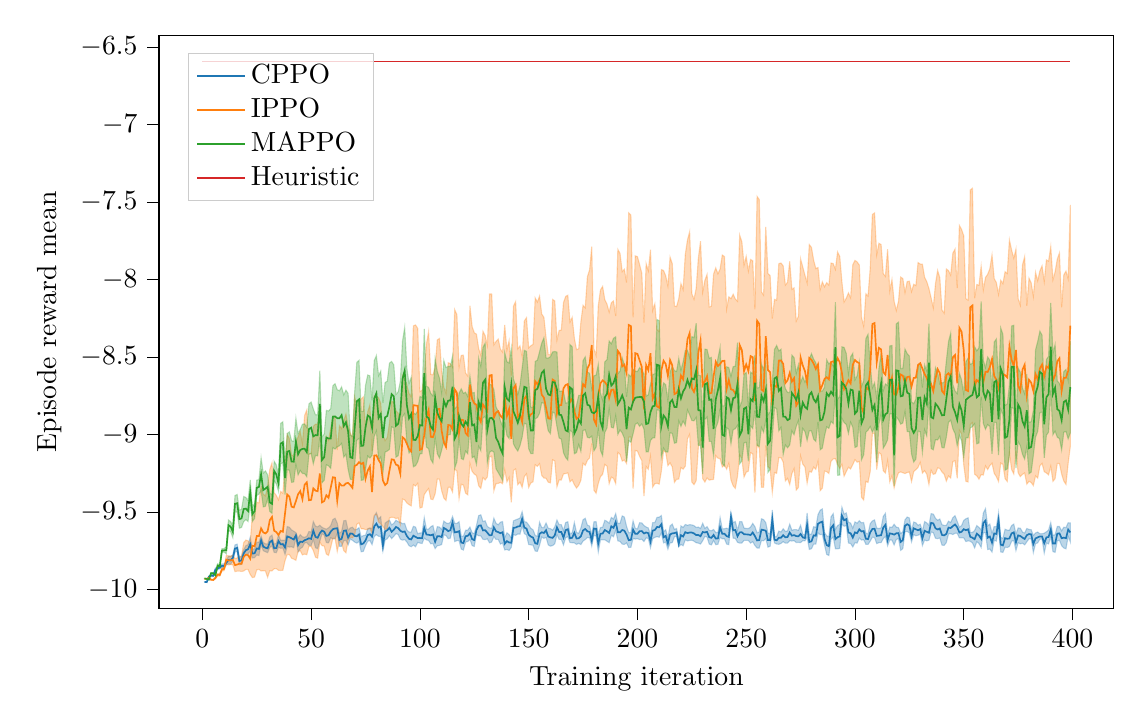
\begin{tikzpicture}

\definecolor{crimson2143940}{RGB}{214,39,40}
\definecolor{darkgray176}{RGB}{176,176,176}
\definecolor{darkorange25512714}{RGB}{255,127,14}
\definecolor{forestgreen4416044}{RGB}{44,160,44}
\definecolor{lightgray204}{RGB}{204,204,204}
\definecolor{steelblue31119180}{RGB}{31,119,180}

\begin{axis}[
scale only axis=true,
width=\linewidth,
height=0.6\linewidth,
legend cell align={left},
legend style={
  fill opacity=0.8,
  draw opacity=1,
  text opacity=1,
  at={(0.03,0.97)},
  anchor=north west,
  draw=lightgray204
},
tick align=outside,
tick pos=left,
x grid style={darkgray176},
xlabel={Training iteration},
xmin=-19.95, xmax=418.95,
xtick style={color=black},
y grid style={darkgray176},
ylabel={Episode reward mean},
ymin=-10.1191891456728, ymax=-6.42540051687272,
ytick style={color=black}
]
\path [draw=steelblue31119180, fill=steelblue31119180, opacity=0.3]
(axis cs:1,-9.94938898144265)
--(axis cs:1,-9.94840928134395)
--(axis cs:2,-9.95035209671428)
--(axis cs:3,-9.91253805241144)
--(axis cs:4,-9.90202635770163)
--(axis cs:5,-9.90353756888012)
--(axis cs:6,-9.8589182979034)
--(axis cs:7,-9.85331823217861)
--(axis cs:8,-9.84725211468432)
--(axis cs:9,-9.83300132943227)
--(axis cs:10,-9.83396863736531)
--(axis cs:11,-9.81155259256815)
--(axis cs:12,-9.78321385755881)
--(axis cs:13,-9.78555650328408)
--(axis cs:14,-9.7752894641988)
--(axis cs:15,-9.71066239779747)
--(axis cs:16,-9.70593071645819)
--(axis cs:17,-9.79024264185695)
--(axis cs:18,-9.78553816338331)
--(axis cs:19,-9.74214216640217)
--(axis cs:20,-9.71587967220406)
--(axis cs:21,-9.70870427529652)
--(axis cs:22,-9.66091020115968)
--(axis cs:23,-9.73748563072518)
--(axis cs:24,-9.73675361188798)
--(axis cs:25,-9.69228446360446)
--(axis cs:26,-9.69382085636659)
--(axis cs:27,-9.65346250948684)
--(axis cs:28,-9.69481353348341)
--(axis cs:29,-9.70381185038673)
--(axis cs:30,-9.70498730054187)
--(axis cs:31,-9.65933635488615)
--(axis cs:32,-9.64743140956558)
--(axis cs:33,-9.70537457516612)
--(axis cs:34,-9.70025596294606)
--(axis cs:35,-9.64548254561372)
--(axis cs:36,-9.68146237751929)
--(axis cs:37,-9.67988369103956)
--(axis cs:38,-9.68220854642292)
--(axis cs:39,-9.59214256696429)
--(axis cs:40,-9.59710740889691)
--(axis cs:41,-9.61398676047009)
--(axis cs:42,-9.62220866268125)
--(axis cs:43,-9.63171057998234)
--(axis cs:44,-9.66809531402744)
--(axis cs:45,-9.64416120611386)
--(axis cs:46,-9.65814844859596)
--(axis cs:47,-9.66227453634962)
--(axis cs:48,-9.65504541042932)
--(axis cs:49,-9.62383248751741)
--(axis cs:50,-9.62842867992628)
--(axis cs:51,-9.55984949484808)
--(axis cs:52,-9.58942268818418)
--(axis cs:53,-9.59425382469327)
--(axis cs:54,-9.58362930122077)
--(axis cs:55,-9.59692988795499)
--(axis cs:56,-9.60392287544621)
--(axis cs:57,-9.60919497045234)
--(axis cs:58,-9.60048237869652)
--(axis cs:59,-9.58579703911419)
--(axis cs:60,-9.54689565091186)
--(axis cs:61,-9.53884646440038)
--(axis cs:62,-9.57042024766873)
--(axis cs:63,-9.63555108421867)
--(axis cs:64,-9.62438974718231)
--(axis cs:65,-9.55513416865643)
--(axis cs:66,-9.55272988939892)
--(axis cs:67,-9.6168035140627)
--(axis cs:68,-9.60108756926079)
--(axis cs:69,-9.59683088313137)
--(axis cs:70,-9.61297254555197)
--(axis cs:71,-9.61062346100014)
--(axis cs:72,-9.59946632574069)
--(axis cs:73,-9.65885274903863)
--(axis cs:74,-9.65040873511323)
--(axis cs:75,-9.64813574990726)
--(axis cs:76,-9.60667452882029)
--(axis cs:77,-9.60148830394564)
--(axis cs:78,-9.60638254688437)
--(axis cs:79,-9.52583865070271)
--(axis cs:80,-9.5027641532681)
--(axis cs:81,-9.54322820594301)
--(axis cs:82,-9.52893302777013)
--(axis cs:83,-9.67772115557755)
--(axis cs:84,-9.5698564244613)
--(axis cs:85,-9.55996102738501)
--(axis cs:86,-9.55130129400135)
--(axis cs:87,-9.5816462166725)
--(axis cs:88,-9.57142109943188)
--(axis cs:89,-9.55160322727955)
--(axis cs:90,-9.56116721616262)
--(axis cs:91,-9.56477013474746)
--(axis cs:92,-9.57402316113843)
--(axis cs:93,-9.57170323326176)
--(axis cs:94,-9.61453830080388)
--(axis cs:95,-9.6276994299424)
--(axis cs:96,-9.62797598681966)
--(axis cs:97,-9.5909330601431)
--(axis cs:98,-9.59567888826327)
--(axis cs:99,-9.63918638002948)
--(axis cs:100,-9.63382649103776)
--(axis cs:101,-9.63319380151234)
--(axis cs:102,-9.53494719996291)
--(axis cs:103,-9.60933467238816)
--(axis cs:104,-9.6089705577274)
--(axis cs:105,-9.59361059374832)
--(axis cs:106,-9.58568791018597)
--(axis cs:107,-9.64729045304473)
--(axis cs:108,-9.59285225751255)
--(axis cs:109,-9.59574433079677)
--(axis cs:110,-9.611834140647)
--(axis cs:111,-9.55712905363405)
--(axis cs:112,-9.5684997512979)
--(axis cs:113,-9.57345435614105)
--(axis cs:114,-9.56480428137683)
--(axis cs:115,-9.52740570329413)
--(axis cs:116,-9.57098823091192)
--(axis cs:117,-9.57219996470822)
--(axis cs:118,-9.56121126882686)
--(axis cs:119,-9.65389933101983)
--(axis cs:120,-9.65432813818263)
--(axis cs:121,-9.61636877256504)
--(axis cs:122,-9.61543916115432)
--(axis cs:123,-9.59573693840882)
--(axis cs:124,-9.6320625517684)
--(axis cs:125,-9.63866231313292)
--(axis cs:126,-9.58556515804991)
--(axis cs:127,-9.52168608199413)
--(axis cs:128,-9.51658084020034)
--(axis cs:129,-9.55991670108842)
--(axis cs:130,-9.55510683748424)
--(axis cs:131,-9.59183828387238)
--(axis cs:132,-9.60125000709859)
--(axis cs:133,-9.60318511459199)
--(axis cs:134,-9.53861841977971)
--(axis cs:135,-9.57173966322369)
--(axis cs:136,-9.5811038047164)
--(axis cs:137,-9.5647172773004)
--(axis cs:138,-9.56014425887634)
--(axis cs:139,-9.66370568556623)
--(axis cs:140,-9.63250937292254)
--(axis cs:141,-9.64358285831168)
--(axis cs:142,-9.66729915308848)
--(axis cs:143,-9.55579130150325)
--(axis cs:144,-9.54914307559262)
--(axis cs:145,-9.54385401250768)
--(axis cs:146,-9.53777430285811)
--(axis cs:147,-9.49699395115151)
--(axis cs:148,-9.56097279256371)
--(axis cs:149,-9.56373946732806)
--(axis cs:150,-9.582087200123)
--(axis cs:151,-9.60362468816798)
--(axis cs:152,-9.61312944000568)
--(axis cs:153,-9.64982752649687)
--(axis cs:154,-9.65513740175475)
--(axis cs:155,-9.56456548496565)
--(axis cs:156,-9.59905935392679)
--(axis cs:157,-9.59851383925076)
--(axis cs:158,-9.56949470612352)
--(axis cs:159,-9.60319512326997)
--(axis cs:160,-9.60574284765367)
--(axis cs:161,-9.6156197426283)
--(axis cs:162,-9.59454498133053)
--(axis cs:163,-9.55062687703521)
--(axis cs:164,-9.57983867499492)
--(axis cs:165,-9.58044711499983)
--(axis cs:166,-9.61779647116723)
--(axis cs:167,-9.5661127277424)
--(axis cs:168,-9.56134670777414)
--(axis cs:169,-9.64006222063891)
--(axis cs:170,-9.63286296772644)
--(axis cs:171,-9.56636884875464)
--(axis cs:172,-9.63128875620854)
--(axis cs:173,-9.63582609787692)
--(axis cs:174,-9.60139335281346)
--(axis cs:175,-9.54873721654875)
--(axis cs:176,-9.53923307130566)
--(axis cs:177,-9.58326465511305)
--(axis cs:178,-9.58900336902945)
--(axis cs:179,-9.64657059196983)
--(axis cs:180,-9.56183404662472)
--(axis cs:181,-9.56025102969533)
--(axis cs:182,-9.64533470538843)
--(axis cs:183,-9.59876305893623)
--(axis cs:184,-9.59607422784376)
--(axis cs:185,-9.55198604513684)
--(axis cs:186,-9.55863930697408)
--(axis cs:187,-9.57137514060342)
--(axis cs:188,-9.5332453875938)
--(axis cs:189,-9.54368519561752)
--(axis cs:190,-9.50840144761823)
--(axis cs:191,-9.5728210512759)
--(axis cs:192,-9.57125833735134)
--(axis cs:193,-9.52369527301939)
--(axis cs:194,-9.5312371554903)
--(axis cs:195,-9.5911248786023)
--(axis cs:196,-9.63303525077626)
--(axis cs:197,-9.63036684403624)
--(axis cs:198,-9.5555588579485)
--(axis cs:199,-9.60441573492026)
--(axis cs:200,-9.60751468885855)
--(axis cs:201,-9.56776562715894)
--(axis cs:202,-9.56896435915461)
--(axis cs:203,-9.58513871545618)
--(axis cs:204,-9.59544834871292)
--(axis cs:205,-9.60130440484574)
--(axis cs:206,-9.64737974737663)
--(axis cs:207,-9.5666639560954)
--(axis cs:208,-9.5668567622737)
--(axis cs:209,-9.53298597692109)
--(axis cs:210,-9.53188245773308)
--(axis cs:211,-9.52153485880079)
--(axis cs:212,-9.62538280985022)
--(axis cs:213,-9.61295810857726)
--(axis cs:214,-9.66477458511842)
--(axis cs:215,-9.58816849373514)
--(axis cs:216,-9.57648593959041)
--(axis cs:217,-9.61113405822529)
--(axis cs:218,-9.60476301609718)
--(axis cs:219,-9.68321725410125)
--(axis cs:220,-9.58825450052881)
--(axis cs:221,-9.59744299582627)
--(axis cs:222,-9.57904788331777)
--(axis cs:223,-9.58405661184551)
--(axis cs:224,-9.58019892121195)
--(axis cs:225,-9.58168816593674)
--(axis cs:226,-9.58644757063083)
--(axis cs:227,-9.59781765145186)
--(axis cs:228,-9.59554632303095)
--(axis cs:229,-9.60451417203307)
--(axis cs:230,-9.57115995421769)
--(axis cs:231,-9.60422896176824)
--(axis cs:232,-9.59290941654391)
--(axis cs:233,-9.61655253181554)
--(axis cs:234,-9.61976154929701)
--(axis cs:235,-9.61123869593444)
--(axis cs:236,-9.63075893334914)
--(axis cs:237,-9.63062533872066)
--(axis cs:238,-9.53443709456824)
--(axis cs:239,-9.60704921898524)
--(axis cs:240,-9.6067022528785)
--(axis cs:241,-9.6027931997028)
--(axis cs:242,-9.60953901470898)
--(axis cs:243,-9.50119776253352)
--(axis cs:244,-9.56666871354541)
--(axis cs:245,-9.55981389831999)
--(axis cs:246,-9.61693233918817)
--(axis cs:247,-9.56023890221054)
--(axis cs:248,-9.56040890089291)
--(axis cs:249,-9.60223406522143)
--(axis cs:250,-9.60430441955756)
--(axis cs:251,-9.60535875214515)
--(axis cs:252,-9.59562840720996)
--(axis cs:253,-9.57182025217714)
--(axis cs:254,-9.59310850379844)
--(axis cs:255,-9.63299261813192)
--(axis cs:256,-9.62741911148654)
--(axis cs:257,-9.54217194333017)
--(axis cs:258,-9.54753688174421)
--(axis cs:259,-9.56781073982241)
--(axis cs:260,-9.63492099583105)
--(axis cs:261,-9.63925631624171)
--(axis cs:262,-9.48587807947116)
--(axis cs:263,-9.65658858770568)
--(axis cs:264,-9.65700357298096)
--(axis cs:265,-9.62157781796263)
--(axis cs:266,-9.62743760031486)
--(axis cs:267,-9.60629995005896)
--(axis cs:268,-9.62407364078546)
--(axis cs:269,-9.620500875476)
--(axis cs:270,-9.57684283494806)
--(axis cs:271,-9.61642023492019)
--(axis cs:272,-9.6118651011564)
--(axis cs:273,-9.61247820043086)
--(axis cs:274,-9.61624737872851)
--(axis cs:275,-9.58390956712145)
--(axis cs:276,-9.64169861394248)
--(axis cs:277,-9.64771770655731)
--(axis cs:278,-9.50489903151801)
--(axis cs:279,-9.64369564737403)
--(axis cs:280,-9.64045297128862)
--(axis cs:281,-9.59301740409809)
--(axis cs:282,-9.59740183003417)
--(axis cs:283,-9.51619834700473)
--(axis cs:284,-9.48696848858212)
--(axis cs:285,-9.47883419613924)
--(axis cs:286,-9.63163014200303)
--(axis cs:287,-9.65212952632784)
--(axis cs:288,-9.65883643921777)
--(axis cs:289,-9.52959609456314)
--(axis cs:290,-9.50923951257346)
--(axis cs:291,-9.61084566257467)
--(axis cs:292,-9.58551890547288)
--(axis cs:293,-9.57884641506574)
--(axis cs:294,-9.46754579409539)
--(axis cs:295,-9.5121056092992)
--(axis cs:296,-9.50470012978647)
--(axis cs:297,-9.56350733091156)
--(axis cs:298,-9.570293483806)
--(axis cs:299,-9.60335076913671)
--(axis cs:300,-9.5624453086523)
--(axis cs:301,-9.57043407313853)
--(axis cs:302,-9.55443500263015)
--(axis cs:303,-9.56799451521822)
--(axis cs:304,-9.56609227462439)
--(axis cs:305,-9.63539680732005)
--(axis cs:306,-9.63959144215386)
--(axis cs:307,-9.57407471748952)
--(axis cs:308,-9.55611518101265)
--(axis cs:309,-9.54966639186946)
--(axis cs:310,-9.6028897835176)
--(axis cs:311,-9.60492525749806)
--(axis cs:312,-9.60093230367477)
--(axis cs:313,-9.52723540055359)
--(axis cs:314,-9.50656718353024)
--(axis cs:315,-9.6425093670916)
--(axis cs:316,-9.59510767168081)
--(axis cs:317,-9.59787238795087)
--(axis cs:318,-9.57754426010662)
--(axis cs:319,-9.59630487916092)
--(axis cs:320,-9.5988582751112)
--(axis cs:321,-9.63735681580777)
--(axis cs:322,-9.62534367144522)
--(axis cs:323,-9.54892969455485)
--(axis cs:324,-9.53075035365273)
--(axis cs:325,-9.53713882224346)
--(axis cs:326,-9.62004947327561)
--(axis cs:327,-9.56302693944885)
--(axis cs:328,-9.56834237996012)
--(axis cs:329,-9.58419501749237)
--(axis cs:330,-9.57745259111529)
--(axis cs:331,-9.62206986486742)
--(axis cs:332,-9.56042675059846)
--(axis cs:333,-9.56851829084494)
--(axis cs:334,-9.58489360443039)
--(axis cs:335,-9.5092936067547)
--(axis cs:336,-9.51188092566402)
--(axis cs:337,-9.53935697455435)
--(axis cs:338,-9.55199766456172)
--(axis cs:339,-9.54393254714884)
--(axis cs:340,-9.58055590775509)
--(axis cs:341,-9.58489780913238)
--(axis cs:342,-9.58412501072266)
--(axis cs:343,-9.55793864433598)
--(axis cs:344,-9.56616954990699)
--(axis cs:345,-9.53487030690605)
--(axis cs:346,-9.52249032506202)
--(axis cs:347,-9.55863626090341)
--(axis cs:348,-9.59627037000378)
--(axis cs:349,-9.58658952057131)
--(axis cs:350,-9.55292888775649)
--(axis cs:351,-9.54219245960653)
--(axis cs:352,-9.53602325515565)
--(axis cs:353,-9.62942470958601)
--(axis cs:354,-9.63085275216704)
--(axis cs:355,-9.61758809389134)
--(axis cs:356,-9.58621957931438)
--(axis cs:357,-9.59757224890071)
--(axis cs:358,-9.61520930619311)
--(axis cs:359,-9.50502821968266)
--(axis cs:360,-9.47647630313493)
--(axis cs:361,-9.58845166079678)
--(axis cs:362,-9.57615185342102)
--(axis cs:363,-9.63554387316546)
--(axis cs:364,-9.59277679002091)
--(axis cs:365,-9.59343442860159)
--(axis cs:366,-9.50316936592195)
--(axis cs:367,-9.66207833204238)
--(axis cs:368,-9.66877765885006)
--(axis cs:369,-9.60962673982229)
--(axis cs:370,-9.61556324208009)
--(axis cs:371,-9.61656699579214)
--(axis cs:372,-9.58593233595011)
--(axis cs:373,-9.5764319256307)
--(axis cs:374,-9.64021242221199)
--(axis cs:375,-9.60155268933225)
--(axis cs:376,-9.60267108387046)
--(axis cs:377,-9.62767605504253)
--(axis cs:378,-9.63412153793183)
--(axis cs:379,-9.60494019960151)
--(axis cs:380,-9.61086908883548)
--(axis cs:381,-9.6126519996278)
--(axis cs:382,-9.65014137815002)
--(axis cs:383,-9.63366774522857)
--(axis cs:384,-9.62769348092157)
--(axis cs:385,-9.63883547021668)
--(axis cs:386,-9.63884833806177)
--(axis cs:387,-9.63529768273552)
--(axis cs:388,-9.62627820465961)
--(axis cs:389,-9.61403972939061)
--(axis cs:390,-9.56679147506099)
--(axis cs:391,-9.64922779305094)
--(axis cs:392,-9.64520186736088)
--(axis cs:393,-9.5917524661124)
--(axis cs:394,-9.59171045689273)
--(axis cs:395,-9.62007603776894)
--(axis cs:396,-9.59659148162303)
--(axis cs:397,-9.59938934231436)
--(axis cs:398,-9.56791292352494)
--(axis cs:399,-9.56899504690559)
--(axis cs:399,-9.69141523967542)
--(axis cs:399,-9.69141523967542)
--(axis cs:398,-9.65557810653902)
--(axis cs:397,-9.73594855962476)
--(axis cs:396,-9.73060327495083)
--(axis cs:395,-9.71527860576862)
--(axis cs:394,-9.68088516909475)
--(axis cs:393,-9.68437586410814)
--(axis cs:392,-9.75875667150085)
--(axis cs:391,-9.75390627340537)
--(axis cs:390,-9.65647348583451)
--(axis cs:389,-9.70470502280537)
--(axis cs:388,-9.69839468563711)
--(axis cs:387,-9.76371071059956)
--(axis cs:386,-9.6737316899945)
--(axis cs:385,-9.67318854387119)
--(axis cs:384,-9.69763677589402)
--(axis cs:383,-9.70342003772067)
--(axis cs:382,-9.7600057718971)
--(axis cs:381,-9.67197428792938)
--(axis cs:380,-9.67041218304494)
--(axis cs:379,-9.69100126557489)
--(axis cs:378,-9.7103306777869)
--(axis cs:377,-9.6999115515196)
--(axis cs:376,-9.70371308495145)
--(axis cs:375,-9.69691400600669)
--(axis cs:374,-9.74731361958592)
--(axis cs:373,-9.68291822610352)
--(axis cs:372,-9.68650682970731)
--(axis cs:371,-9.72129347726008)
--(axis cs:370,-9.72741914763986)
--(axis cs:369,-9.72520835748784)
--(axis cs:368,-9.75922057758427)
--(axis cs:367,-9.75592821643023)
--(axis cs:366,-9.59958799112603)
--(axis cs:365,-9.6859350831062)
--(axis cs:364,-9.68081556541166)
--(axis cs:363,-9.7567460469668)
--(axis cs:362,-9.7370072847626)
--(axis cs:361,-9.74056636066698)
--(axis cs:360,-9.63089483250058)
--(axis cs:359,-9.63331365409375)
--(axis cs:358,-9.72718993821056)
--(axis cs:357,-9.70208337939884)
--(axis cs:356,-9.68991208921899)
--(axis cs:355,-9.72990478799108)
--(axis cs:354,-9.69792503714506)
--(axis cs:353,-9.68733216562077)
--(axis cs:352,-9.68453743590712)
--(axis cs:351,-9.68913057753478)
--(axis cs:350,-9.6657269444114)
--(axis cs:349,-9.66556131154944)
--(axis cs:348,-9.66540216106972)
--(axis cs:347,-9.63535511879254)
--(axis cs:346,-9.63533342254969)
--(axis cs:345,-9.64394422509207)
--(axis cs:344,-9.63813620581669)
--(axis cs:343,-9.64004685031133)
--(axis cs:342,-9.69554364044067)
--(axis cs:341,-9.71369471952706)
--(axis cs:340,-9.7123316099099)
--(axis cs:339,-9.66558273423494)
--(axis cs:338,-9.67072209901775)
--(axis cs:337,-9.66745635139159)
--(axis cs:336,-9.63189567532187)
--(axis cs:335,-9.62740088144714)
--(axis cs:334,-9.68033496827647)
--(axis cs:333,-9.68458751146756)
--(axis cs:332,-9.67913976557581)
--(axis cs:331,-9.71480886408195)
--(axis cs:330,-9.64007496350766)
--(axis cs:329,-9.64844912493973)
--(axis cs:328,-9.65145874655144)
--(axis cs:327,-9.64481027135544)
--(axis cs:326,-9.69174234701216)
--(axis cs:325,-9.63295892293336)
--(axis cs:324,-9.62361245873548)
--(axis cs:323,-9.62674827708361)
--(axis cs:322,-9.73453529883176)
--(axis cs:321,-9.74572654151271)
--(axis cs:320,-9.6701762610634)
--(axis cs:319,-9.67544189667297)
--(axis cs:318,-9.71098480466269)
--(axis cs:317,-9.67996835116521)
--(axis cs:316,-9.67812835562138)
--(axis cs:315,-9.71627021039503)
--(axis cs:314,-9.65573504892895)
--(axis cs:313,-9.67073401779315)
--(axis cs:312,-9.69582180948779)
--(axis cs:311,-9.6961489968802)
--(axis cs:310,-9.70236152892021)
--(axis cs:309,-9.66288392278296)
--(axis cs:308,-9.66054562487469)
--(axis cs:307,-9.68667462894051)
--(axis cs:306,-9.70736571574194)
--(axis cs:305,-9.70641227543039)
--(axis cs:304,-9.6771195352525)
--(axis cs:303,-9.67941416681382)
--(axis cs:302,-9.66584013876779)
--(axis cs:301,-9.69889239263703)
--(axis cs:300,-9.69720579977271)
--(axis cs:299,-9.72377663177833)
--(axis cs:298,-9.70148376835153)
--(axis cs:297,-9.69864676956848)
--(axis cs:296,-9.58455418285297)
--(axis cs:295,-9.59074358606287)
--(axis cs:294,-9.5754139639291)
--(axis cs:293,-9.73272503387629)
--(axis cs:292,-9.73624711537368)
--(axis cs:291,-9.73562056147093)
--(axis cs:290,-9.65881674470675)
--(axis cs:289,-9.67338484439941)
--(axis cs:288,-9.77927623181809)
--(axis cs:287,-9.77180583407672)
--(axis cs:286,-9.71224322510286)
--(axis cs:285,-9.64207118694515)
--(axis cs:284,-9.6447784549233)
--(axis cs:283,-9.63359457450045)
--(axis cs:282,-9.70588894156776)
--(axis cs:281,-9.7054727803474)
--(axis cs:280,-9.73524961139604)
--(axis cs:279,-9.73971372748947)
--(axis cs:278,-9.66029544232359)
--(axis cs:277,-9.68483086091327)
--(axis cs:276,-9.68289469490491)
--(axis cs:275,-9.69572220635841)
--(axis cs:274,-9.69465060404186)
--(axis cs:273,-9.69507965152916)
--(axis cs:272,-9.68325325710714)
--(axis cs:271,-9.68577517395286)
--(axis cs:270,-9.68395155709725)
--(axis cs:269,-9.69875125029386)
--(axis cs:268,-9.69944932532817)
--(axis cs:267,-9.68968916227023)
--(axis cs:266,-9.70099620711531)
--(axis cs:265,-9.70685778635993)
--(axis cs:264,-9.70479630012025)
--(axis cs:263,-9.69813778863828)
--(axis cs:262,-9.61021320243174)
--(axis cs:261,-9.71983243071329)
--(axis cs:260,-9.72496782071881)
--(axis cs:259,-9.6692312361269)
--(axis cs:258,-9.68417952108283)
--(axis cs:257,-9.68172039988313)
--(axis cs:256,-9.7308543523049)
--(axis cs:255,-9.73068929338481)
--(axis cs:254,-9.71456544806687)
--(axis cs:253,-9.68958203668443)
--(axis cs:252,-9.69899394215745)
--(axis cs:251,-9.68209406687471)
--(axis cs:250,-9.68152618045577)
--(axis cs:249,-9.68136095958067)
--(axis cs:248,-9.69845571729093)
--(axis cs:247,-9.69912342983805)
--(axis cs:246,-9.69390313080025)
--(axis cs:245,-9.66858300776698)
--(axis cs:244,-9.66726740819362)
--(axis cs:243,-9.56228887607046)
--(axis cs:242,-9.70906447146967)
--(axis cs:241,-9.7052385968396)
--(axis cs:240,-9.67059293653443)
--(axis cs:239,-9.67201090752986)
--(axis cs:238,-9.66102407487319)
--(axis cs:237,-9.70658815790311)
--(axis cs:236,-9.70926137405526)
--(axis cs:235,-9.68196905999446)
--(axis cs:234,-9.71033133470297)
--(axis cs:233,-9.70579515156809)
--(axis cs:232,-9.65946415282789)
--(axis cs:231,-9.65624510442143)
--(axis cs:230,-9.68387405587649)
--(axis cs:229,-9.7049706012907)
--(axis cs:228,-9.69910293459119)
--(axis cs:227,-9.69677059200328)
--(axis cs:226,-9.68666357642188)
--(axis cs:225,-9.6803378328737)
--(axis cs:224,-9.68195233263649)
--(axis cs:223,-9.68525966483647)
--(axis cs:222,-9.67819485118309)
--(axis cs:221,-9.71617391881526)
--(axis cs:220,-9.70755432971793)
--(axis cs:219,-9.72328482150419)
--(axis cs:218,-9.65470848150476)
--(axis cs:217,-9.65809337975153)
--(axis cs:216,-9.69623543697767)
--(axis cs:215,-9.69758903140331)
--(axis cs:214,-9.73829972122692)
--(axis cs:213,-9.69260491209995)
--(axis cs:212,-9.69781266217743)
--(axis cs:211,-9.63339583603423)
--(axis cs:210,-9.66138481406296)
--(axis cs:209,-9.65744095041906)
--(axis cs:208,-9.66206039767356)
--(axis cs:207,-9.67000346419284)
--(axis cs:206,-9.72916932379866)
--(axis cs:205,-9.66903449021852)
--(axis cs:204,-9.6654616769124)
--(axis cs:203,-9.68888784747355)
--(axis cs:202,-9.67399911648418)
--(axis cs:201,-9.676339611675)
--(axis cs:200,-9.67027461216516)
--(axis cs:199,-9.6730460989522)
--(axis cs:198,-9.66865218480702)
--(axis cs:197,-9.72573641139793)
--(axis cs:196,-9.72749502830037)
--(axis cs:195,-9.69756253568043)
--(axis cs:194,-9.70735224883853)
--(axis cs:193,-9.70563638291289)
--(axis cs:192,-9.68800577809977)
--(axis cs:191,-9.68494293500153)
--(axis cs:190,-9.61655830271557)
--(axis cs:189,-9.65798652280771)
--(axis cs:188,-9.64875231032732)
--(axis cs:187,-9.69620192048558)
--(axis cs:186,-9.6866962989817)
--(axis cs:185,-9.67782945768236)
--(axis cs:184,-9.67788427264335)
--(axis cs:183,-9.67839865054083)
--(axis cs:182,-9.75681583860887)
--(axis cs:181,-9.6529403951985)
--(axis cs:180,-9.64836937009411)
--(axis cs:179,-9.71843443487757)
--(axis cs:178,-9.66496505452998)
--(axis cs:177,-9.66286504919858)
--(axis cs:176,-9.67636807452227)
--(axis cs:175,-9.68573492906657)
--(axis cs:174,-9.70844448089314)
--(axis cs:173,-9.7006180573451)
--(axis cs:172,-9.70737082363554)
--(axis cs:171,-9.69772397896562)
--(axis cs:170,-9.69650690893976)
--(axis cs:169,-9.69614257004811)
--(axis cs:168,-9.65802135275923)
--(axis cs:167,-9.66413095733513)
--(axis cs:166,-9.71107999220576)
--(axis cs:165,-9.67384447555999)
--(axis cs:164,-9.6755246323982)
--(axis cs:163,-9.64371848290535)
--(axis cs:162,-9.70360654750891)
--(axis cs:161,-9.714989615391)
--(axis cs:160,-9.7187667294228)
--(axis cs:159,-9.71085382048228)
--(axis cs:158,-9.66208719992723)
--(axis cs:157,-9.66865099146784)
--(axis cs:156,-9.65919057779188)
--(axis cs:155,-9.71401931277164)
--(axis cs:154,-9.75231924060557)
--(axis cs:153,-9.75016247088913)
--(axis cs:152,-9.71308289674647)
--(axis cs:151,-9.71047023160373)
--(axis cs:150,-9.70801189941415)
--(axis cs:149,-9.6473322858427)
--(axis cs:148,-9.63735420354136)
--(axis cs:147,-9.58884775913105)
--(axis cs:146,-9.64162443199291)
--(axis cs:145,-9.64044395031365)
--(axis cs:144,-9.64849199708405)
--(axis cs:143,-9.64564353729789)
--(axis cs:142,-9.72659725914955)
--(axis cs:141,-9.74673738667861)
--(axis cs:140,-9.74000127011526)
--(axis cs:139,-9.74320917079624)
--(axis cs:138,-9.69817384804898)
--(axis cs:137,-9.70523473360621)
--(axis cs:136,-9.6748212592629)
--(axis cs:135,-9.67529551863758)
--(axis cs:134,-9.65663876566553)
--(axis cs:133,-9.69199538672914)
--(axis cs:132,-9.69706254266529)
--(axis cs:131,-9.67185020249457)
--(axis cs:130,-9.67653438080549)
--(axis cs:129,-9.67472675122086)
--(axis cs:128,-9.65255302667602)
--(axis cs:127,-9.65211936076098)
--(axis cs:126,-9.6430173588577)
--(axis cs:125,-9.72044337628092)
--(axis cs:124,-9.71499290644094)
--(axis cs:123,-9.67475408866608)
--(axis cs:122,-9.68881816909858)
--(axis cs:121,-9.69290845813619)
--(axis cs:120,-9.74361708273483)
--(axis cs:119,-9.73725034153474)
--(axis cs:118,-9.68320993303471)
--(axis cs:117,-9.6830333888503)
--(axis cs:116,-9.68925532250626)
--(axis cs:115,-9.60273691531902)
--(axis cs:114,-9.66715390148706)
--(axis cs:113,-9.67037734129213)
--(axis cs:112,-9.65023294989026)
--(axis cs:111,-9.64544086455988)
--(axis cs:110,-9.70783070121143)
--(axis cs:109,-9.71411936564925)
--(axis cs:108,-9.71586112803386)
--(axis cs:107,-9.73456141941902)
--(axis cs:106,-9.7006296238758)
--(axis cs:105,-9.70385225621137)
--(axis cs:104,-9.6815531452136)
--(axis cs:103,-9.67825818222997)
--(axis cs:102,-9.66702961002406)
--(axis cs:101,-9.70165283092689)
--(axis cs:100,-9.69901318339069)
--(axis cs:99,-9.69442755995049)
--(axis cs:98,-9.72204857234131)
--(axis cs:97,-9.71170169969749)
--(axis cs:96,-9.72239851593521)
--(axis cs:95,-9.71566361061131)
--(axis cs:94,-9.69131264984792)
--(axis cs:93,-9.67614645265223)
--(axis cs:92,-9.68001160253793)
--(axis cs:91,-9.67367871411419)
--(axis cs:90,-9.6433051865317)
--(axis cs:89,-9.63795999016828)
--(axis cs:88,-9.65509943952736)
--(axis cs:87,-9.6701783495941)
--(axis cs:86,-9.65032725289315)
--(axis cs:85,-9.67120636270074)
--(axis cs:84,-9.67886152354833)
--(axis cs:83,-9.75138648284764)
--(axis cs:82,-9.65693810028482)
--(axis cs:81,-9.65488767320937)
--(axis cs:80,-9.64438739166211)
--(axis cs:79,-9.65708300495016)
--(axis cs:78,-9.70860215858293)
--(axis cs:77,-9.68184654131332)
--(axis cs:76,-9.68757913073937)
--(axis cs:75,-9.71539588911611)
--(axis cs:74,-9.75209685457725)
--(axis cs:73,-9.75513072438196)
--(axis cs:72,-9.68685202593538)
--(axis cs:71,-9.69941379746474)
--(axis cs:70,-9.69242046344617)
--(axis cs:69,-9.68099886759525)
--(axis cs:68,-9.67219336823978)
--(axis cs:67,-9.71105194315277)
--(axis cs:66,-9.68125781021571)
--(axis cs:65,-9.68425359284755)
--(axis cs:64,-9.71940537371177)
--(axis cs:63,-9.71986613186588)
--(axis cs:62,-9.63582779946339)
--(axis cs:61,-9.67099565248617)
--(axis cs:60,-9.67243317366113)
--(axis cs:59,-9.66412156889366)
--(axis cs:58,-9.6968858826209)
--(axis cs:57,-9.69623329465439)
--(axis cs:56,-9.64712840963855)
--(axis cs:55,-9.63897839435347)
--(axis cs:54,-9.68645237284277)
--(axis cs:53,-9.73501153539803)
--(axis cs:52,-9.72924204771899)
--(axis cs:51,-9.67658255357075)
--(axis cs:50,-9.71517236903914)
--(axis cs:49,-9.71225231722171)
--(axis cs:48,-9.695547052968)
--(axis cs:47,-9.69857001042848)
--(axis cs:46,-9.7253315251365)
--(axis cs:45,-9.73466599808544)
--(axis cs:44,-9.75585415440935)
--(axis cs:43,-9.666308263462)
--(axis cs:42,-9.72899780615506)
--(axis cs:41,-9.72278975445991)
--(axis cs:40,-9.72479654352948)
--(axis cs:39,-9.71959985733662)
--(axis cs:38,-9.77289117613299)
--(axis cs:37,-9.73048957636352)
--(axis cs:36,-9.73258114922798)
--(axis cs:35,-9.7254340856272)
--(axis cs:34,-9.76116081403307)
--(axis cs:33,-9.75911468636308)
--(axis cs:32,-9.71782471653523)
--(axis cs:31,-9.72689240710744)
--(axis cs:30,-9.76072480296793)
--(axis cs:29,-9.75473305844147)
--(axis cs:28,-9.74806083982418)
--(axis cs:27,-9.70852157909028)
--(axis cs:26,-9.77967199966325)
--(axis cs:25,-9.77492784669354)
--(axis cs:24,-9.79318951556617)
--(axis cs:23,-9.79495600178222)
--(axis cs:22,-9.75168043600958)
--(axis cs:21,-9.76834141029031)
--(axis cs:20,-9.77397328837096)
--(axis cs:19,-9.78873222340366)
--(axis cs:18,-9.8362727260222)
--(axis cs:17,-9.83835536008385)
--(axis cs:16,-9.75320079990073)
--(axis cs:15,-9.75750987438692)
--(axis cs:14,-9.81396284834383)
--(axis cs:13,-9.83541248572972)
--(axis cs:12,-9.83269175450158)
--(axis cs:11,-9.84017156958983)
--(axis cs:10,-9.85901879798302)
--(axis cs:9,-9.85880476316734)
--(axis cs:8,-9.86482906476067)
--(axis cs:7,-9.87009961000861)
--(axis cs:6,-9.88154064866819)
--(axis cs:5,-9.91533601926466)
--(axis cs:4,-9.91461926758721)
--(axis cs:3,-9.91759139944858)
--(axis cs:2,-9.95128966254556)
--(axis cs:1,-9.94938898144265)
--cycle;

\path [draw=darkorange25512714, fill=darkorange25512714, opacity=0.3]
(axis cs:1,-9.93046713051996)
--(axis cs:1,-9.92868195389357)
--(axis cs:2,-9.92867313582447)
--(axis cs:3,-9.92171988142691)
--(axis cs:4,-9.93258226671579)
--(axis cs:5,-9.93404950850982)
--(axis cs:6,-9.91734076894389)
--(axis cs:7,-9.89549736237979)
--(axis cs:8,-9.89662237118142)
--(axis cs:9,-9.85737936946578)
--(axis cs:10,-9.85327354379832)
--(axis cs:11,-9.77804320250998)
--(axis cs:12,-9.78169321135112)
--(axis cs:13,-9.782390757031)
--(axis cs:14,-9.77697211052809)
--(axis cs:15,-9.79867001045821)
--(axis cs:16,-9.79538360547523)
--(axis cs:17,-9.78269109234814)
--(axis cs:18,-9.78383909050266)
--(axis cs:19,-9.69588391209497)
--(axis cs:20,-9.67960508084912)
--(axis cs:21,-9.68455049674207)
--(axis cs:22,-9.69861986692433)
--(axis cs:23,-9.51087324136066)
--(axis cs:24,-9.52222238939571)
--(axis cs:25,-9.43547763532567)
--(axis cs:26,-9.44002982445434)
--(axis cs:27,-9.32869552344854)
--(axis cs:28,-9.38358556838697)
--(axis cs:29,-9.39456005396215)
--(axis cs:30,-9.32618943179119)
--(axis cs:31,-9.22447059895184)
--(axis cs:32,-9.1816778349037)
--(axis cs:33,-9.37368239207241)
--(axis cs:34,-9.39210465409235)
--(axis cs:35,-9.41980151562093)
--(axis cs:36,-9.3661459892909)
--(axis cs:37,-9.37817679034054)
--(axis cs:38,-9.20340147784809)
--(axis cs:39,-8.99870005466454)
--(axis cs:40,-9.02485366858482)
--(axis cs:41,-9.13182512207328)
--(axis cs:42,-9.13594405129504)
--(axis cs:43,-9.04804218506664)
--(axis cs:44,-9.0141318930304)
--(axis cs:45,-8.97891836386347)
--(axis cs:46,-9.05686846932412)
--(axis cs:47,-8.87601774821754)
--(axis cs:48,-8.84018761942975)
--(axis cs:49,-9.12605346304792)
--(axis cs:50,-9.11899993909596)
--(axis cs:51,-8.94624141778904)
--(axis cs:52,-8.93216246134364)
--(axis cs:53,-8.93349744268778)
--(axis cs:54,-8.80873872281465)
--(axis cs:55,-9.1566287124448)
--(axis cs:56,-9.13799476951771)
--(axis cs:57,-9.01042850683953)
--(axis cs:58,-9.03524283101981)
--(axis cs:59,-8.95833690369758)
--(axis cs:60,-8.88094737122655)
--(axis cs:61,-8.88647666711209)
--(axis cs:62,-9.09960866769962)
--(axis cs:63,-8.94120416225815)
--(axis cs:64,-8.96098478793366)
--(axis cs:65,-8.90934787838746)
--(axis cs:66,-8.86654117234569)
--(axis cs:67,-8.94294321632362)
--(axis cs:68,-8.9877392915895)
--(axis cs:69,-9.02071758915654)
--(axis cs:70,-8.7549738953648)
--(axis cs:71,-8.81246199937654)
--(axis cs:72,-8.78578330580132)
--(axis cs:73,-8.76975842179216)
--(axis cs:74,-8.75619280834501)
--(axis cs:75,-8.95637955128056)
--(axis cs:76,-8.85263764893645)
--(axis cs:77,-8.80625568068145)
--(axis cs:78,-9.10410734058767)
--(axis cs:79,-8.74979312211446)
--(axis cs:80,-8.75091936860893)
--(axis cs:81,-8.76213752977202)
--(axis cs:82,-8.79687557779684)
--(axis cs:83,-8.9988376691176)
--(axis cs:84,-9.03835921193967)
--(axis cs:85,-9.0183776820796)
--(axis cs:86,-8.92571105044843)
--(axis cs:87,-8.78557754641325)
--(axis cs:88,-8.78938033510015)
--(axis cs:89,-8.84537865098996)
--(axis cs:90,-8.86016505662632)
--(axis cs:91,-8.92550636472335)
--(axis cs:92,-8.61761579249758)
--(axis cs:93,-8.63517126551817)
--(axis cs:94,-8.67746579906972)
--(axis cs:95,-8.73437372997561)
--(axis cs:96,-8.75531583632019)
--(axis cs:97,-8.29789925677534)
--(axis cs:98,-8.29248767030585)
--(axis cs:99,-8.31447229066751)
--(axis cs:100,-8.72280182775994)
--(axis cs:101,-8.71375464943744)
--(axis cs:102,-8.61787883561347)
--(axis cs:103,-8.41678250763485)
--(axis cs:104,-8.33439064102968)
--(axis cs:105,-8.61162024872621)
--(axis cs:106,-8.61371811038667)
--(axis cs:107,-8.56631381424354)
--(axis cs:108,-8.3881404085283)
--(axis cs:109,-8.37947488295124)
--(axis cs:110,-8.58807783258364)
--(axis cs:111,-8.69277631954725)
--(axis cs:112,-8.73359861974382)
--(axis cs:113,-8.53631463967432)
--(axis cs:114,-8.5413070686995)
--(axis cs:115,-8.56328749833262)
--(axis cs:116,-8.19412280053098)
--(axis cs:117,-8.22521178520073)
--(axis cs:118,-8.56304676798399)
--(axis cs:119,-8.48820794936828)
--(axis cs:120,-8.48797315937531)
--(axis cs:121,-8.60246334077434)
--(axis cs:122,-8.6219741083685)
--(axis cs:123,-8.16881262564797)
--(axis cs:124,-8.30189613036837)
--(axis cs:125,-8.3430351401449)
--(axis cs:126,-8.35193366840821)
--(axis cs:127,-8.44364586816504)
--(axis cs:128,-8.48885995265759)
--(axis cs:129,-8.33389992927797)
--(axis cs:130,-8.36119224185892)
--(axis cs:131,-8.42374558350138)
--(axis cs:132,-8.0930018913621)
--(axis cs:133,-8.09261575302738)
--(axis cs:134,-8.42098099268355)
--(axis cs:135,-8.39903776296746)
--(axis cs:136,-8.38338560342521)
--(axis cs:137,-8.447823287066)
--(axis cs:138,-8.46810798190788)
--(axis cs:139,-8.29303006924421)
--(axis cs:140,-8.45507163698078)
--(axis cs:141,-8.39386205385738)
--(axis cs:142,-8.61850420271177)
--(axis cs:143,-8.1713612919429)
--(axis cs:144,-8.14177802494519)
--(axis cs:145,-8.44692779608653)
--(axis cs:146,-8.42722131470359)
--(axis cs:147,-8.49509739976579)
--(axis cs:148,-8.26638861990424)
--(axis cs:149,-8.24567266509062)
--(axis cs:150,-8.44093987120354)
--(axis cs:151,-8.42689843708267)
--(axis cs:152,-8.4176324790187)
--(axis cs:153,-8.11854962364535)
--(axis cs:154,-8.14482002534999)
--(axis cs:155,-8.10585557002026)
--(axis cs:156,-8.22198376293136)
--(axis cs:157,-8.24324521883155)
--(axis cs:158,-8.37467314833092)
--(axis cs:159,-8.48291821076847)
--(axis cs:160,-8.48497741291534)
--(axis cs:161,-8.12794914237882)
--(axis cs:162,-8.13760522124892)
--(axis cs:163,-8.38994759326893)
--(axis cs:164,-8.32807203132071)
--(axis cs:165,-8.32507947494569)
--(axis cs:166,-8.14899245805553)
--(axis cs:167,-8.10847098205623)
--(axis cs:168,-8.10127476527755)
--(axis cs:169,-8.27405856015996)
--(axis cs:170,-8.24378301276728)
--(axis cs:171,-8.37733711948326)
--(axis cs:172,-8.45203251218406)
--(axis cs:173,-8.44593248993534)
--(axis cs:174,-8.27253015499097)
--(axis cs:175,-8.16564974532531)
--(axis cs:176,-8.18237492298277)
--(axis cs:177,-7.98073941755314)
--(axis cs:178,-7.93781012894287)
--(axis cs:179,-7.78759058848821)
--(axis cs:180,-8.44761020683789)
--(axis cs:181,-8.48929999305876)
--(axis cs:182,-8.16856079154273)
--(axis cs:183,-8.06691400315741)
--(axis cs:184,-8.04397199520225)
--(axis cs:185,-8.12941345072184)
--(axis cs:186,-8.15837776000397)
--(axis cs:187,-8.20960417253662)
--(axis cs:188,-8.14900010951933)
--(axis cs:189,-8.13699571124362)
--(axis cs:190,-8.23557843501294)
--(axis cs:191,-7.80523810223485)
--(axis cs:192,-7.83075871370724)
--(axis cs:193,-7.94928943871859)
--(axis cs:194,-7.93327242545332)
--(axis cs:195,-8.01920709969514)
--(axis cs:196,-7.5695837757206)
--(axis cs:197,-7.58432871003714)
--(axis cs:198,-8.24300583544454)
--(axis cs:199,-7.8471669824845)
--(axis cs:200,-7.85194803706766)
--(axis cs:201,-7.90275001918364)
--(axis cs:202,-7.9586485530728)
--(axis cs:203,-8.27681903066586)
--(axis cs:204,-7.89709670979862)
--(axis cs:205,-7.94369940389323)
--(axis cs:206,-7.80768492625962)
--(axis cs:207,-8.19923420804579)
--(axis cs:208,-8.15569706408162)
--(axis cs:209,-8.32240034224264)
--(axis cs:210,-8.33448354324798)
--(axis cs:211,-7.93525473064276)
--(axis cs:212,-7.94139885775463)
--(axis cs:213,-7.97565726573085)
--(axis cs:214,-8.0417993724595)
--(axis cs:215,-7.85540286786413)
--(axis cs:216,-7.89646373669599)
--(axis cs:217,-8.16965913417101)
--(axis cs:218,-8.17385899669449)
--(axis cs:219,-8.12213121943827)
--(axis cs:220,-8.02591247157381)
--(axis cs:221,-8.06385675400274)
--(axis cs:222,-7.83733979655991)
--(axis cs:223,-7.74456548786552)
--(axis cs:224,-7.69134565742691)
--(axis cs:225,-8.0912606777308)
--(axis cs:226,-8.12687536203954)
--(axis cs:227,-8.05704931387286)
--(axis cs:228,-7.86260592666496)
--(axis cs:229,-7.75220286377696)
--(axis cs:230,-8.08051291343023)
--(axis cs:231,-8.00495179718669)
--(axis cs:232,-7.9663783968421)
--(axis cs:233,-8.17639519024725)
--(axis cs:234,-8.17142255024088)
--(axis cs:235,-7.96443590177692)
--(axis cs:236,-7.92454725673893)
--(axis cs:237,-7.96290812448195)
--(axis cs:238,-7.93180985463795)
--(axis cs:239,-7.84180299398502)
--(axis cs:240,-7.85114000181203)
--(axis cs:241,-8.18940414565049)
--(axis cs:242,-8.11111399503977)
--(axis cs:243,-8.12294973770938)
--(axis cs:244,-8.09414820592398)
--(axis cs:245,-8.1253546261514)
--(axis cs:246,-8.13955814516515)
--(axis cs:247,-7.71321151795063)
--(axis cs:248,-7.75568812130979)
--(axis cs:249,-7.9064913587681)
--(axis cs:250,-7.85053198329124)
--(axis cs:251,-7.94479471245394)
--(axis cs:252,-7.87030112077662)
--(axis cs:253,-7.87794567648645)
--(axis cs:254,-8.19198552701122)
--(axis cs:255,-7.46367162166448)
--(axis cs:256,-7.48421757158768)
--(axis cs:257,-8.07919884350026)
--(axis cs:258,-8.10043548508417)
--(axis cs:259,-7.6595575212858)
--(axis cs:260,-7.96116146846917)
--(axis cs:261,-7.97415310738801)
--(axis cs:262,-8.25119320366453)
--(axis cs:263,-8.12739904301812)
--(axis cs:264,-8.13302943955738)
--(axis cs:265,-7.89675358681342)
--(axis cs:266,-7.8931965092058)
--(axis cs:267,-7.91159202943043)
--(axis cs:268,-8.03589615430106)
--(axis cs:269,-8.01721069955116)
--(axis cs:270,-7.88206382224384)
--(axis cs:271,-8.063442673495)
--(axis cs:272,-8.05325142469029)
--(axis cs:273,-8.26739044585074)
--(axis cs:274,-8.23705497863603)
--(axis cs:275,-7.86598823184973)
--(axis cs:276,-7.91844050828955)
--(axis cs:277,-7.97149485722134)
--(axis cs:278,-8.02191230478467)
--(axis cs:279,-7.7737527925589)
--(axis cs:280,-7.79280203484022)
--(axis cs:281,-7.87454248090318)
--(axis cs:282,-7.92933866418219)
--(axis cs:283,-7.92219496986694)
--(axis cs:284,-8.06598901476369)
--(axis cs:285,-8.01477751218145)
--(axis cs:286,-8.04654042853819)
--(axis cs:287,-8.0196658687316)
--(axis cs:288,-8.03578454345343)
--(axis cs:289,-7.89310595087909)
--(axis cs:290,-7.89709341216502)
--(axis cs:291,-7.93389955226097)
--(axis cs:292,-7.82208770209723)
--(axis cs:293,-7.8495209525779)
--(axis cs:294,-8.01489484540458)
--(axis cs:295,-8.14432333051565)
--(axis cs:296,-8.11986267172934)
--(axis cs:297,-8.08595427134583)
--(axis cs:298,-8.1178249148854)
--(axis cs:299,-7.90450125184866)
--(axis cs:300,-7.87642865720686)
--(axis cs:301,-7.88618964003642)
--(axis cs:302,-7.90625719854225)
--(axis cs:303,-8.24259052541611)
--(axis cs:304,-8.30131535096049)
--(axis cs:305,-8.09193331319379)
--(axis cs:306,-8.10601167571741)
--(axis cs:307,-7.92868419808792)
--(axis cs:308,-7.57989793423833)
--(axis cs:309,-7.57029168970892)
--(axis cs:310,-7.84040730266855)
--(axis cs:311,-7.76606604938812)
--(axis cs:312,-7.77342526311955)
--(axis cs:313,-7.96116187638516)
--(axis cs:314,-7.978997120019)
--(axis cs:315,-7.80364625518908)
--(axis cs:316,-8.07292717331777)
--(axis cs:317,-7.99992826769326)
--(axis cs:318,-8.1401828438804)
--(axis cs:319,-8.19907611772597)
--(axis cs:320,-8.14052656841052)
--(axis cs:321,-7.98374789353032)
--(axis cs:322,-7.99315809900667)
--(axis cs:323,-8.08323084634157)
--(axis cs:324,-8.01259783748015)
--(axis cs:325,-8.01039186833568)
--(axis cs:326,-8.07717947367768)
--(axis cs:327,-8.03028632182258)
--(axis cs:328,-8.03881258404723)
--(axis cs:329,-7.89035295655156)
--(axis cs:330,-7.89970378640099)
--(axis cs:331,-7.90102293699193)
--(axis cs:332,-7.98582492689162)
--(axis cs:333,-8.01283841808658)
--(axis cs:334,-8.05739302920125)
--(axis cs:335,-8.117360621006)
--(axis cs:336,-8.18153551891303)
--(axis cs:337,-8.02721169819384)
--(axis cs:338,-7.94090364052941)
--(axis cs:339,-7.98792881722567)
--(axis cs:340,-8.19667896936423)
--(axis cs:341,-8.21681391913918)
--(axis cs:342,-7.9313312511825)
--(axis cs:343,-7.94192012727915)
--(axis cs:344,-7.97174152034441)
--(axis cs:345,-7.82913519314249)
--(axis cs:346,-7.80351456769324)
--(axis cs:347,-8.05528491813706)
--(axis cs:348,-7.65084289624788)
--(axis cs:349,-7.67602057401001)
--(axis cs:350,-7.71692764178379)
--(axis cs:351,-8.12290361285815)
--(axis cs:352,-8.13249407293772)
--(axis cs:353,-7.42181687287131)
--(axis cs:354,-7.4112185305967)
--(axis cs:355,-8.12011712297552)
--(axis cs:356,-8.03164190639161)
--(axis cs:357,-8.03649150660764)
--(axis cs:358,-7.91386271106658)
--(axis cs:359,-8.06596485900838)
--(axis cs:360,-7.9862528298424)
--(axis cs:361,-7.96588673588663)
--(axis cs:362,-7.92997929176581)
--(axis cs:363,-7.84106271800017)
--(axis cs:364,-7.99369658512137)
--(axis cs:365,-8.01959619058011)
--(axis cs:366,-8.09526224167466)
--(axis cs:367,-8.00416166374617)
--(axis cs:368,-8.02590591371784)
--(axis cs:369,-7.94888660818713)
--(axis cs:370,-7.9603244677558)
--(axis cs:371,-7.74389743967521)
--(axis cs:372,-7.8093814231894)
--(axis cs:373,-7.86197053199861)
--(axis cs:374,-7.803392811432)
--(axis cs:375,-8.1214025478454)
--(axis cs:376,-8.16519023814032)
--(axis cs:377,-7.90550726083294)
--(axis cs:378,-7.8518568481953)
--(axis cs:379,-8.16974363198022)
--(axis cs:380,-7.99072052246005)
--(axis cs:381,-8.0202908086424)
--(axis cs:382,-8.10789629497477)
--(axis cs:383,-7.95322689306024)
--(axis cs:384,-8.00757842801489)
--(axis cs:385,-7.94387393232474)
--(axis cs:386,-7.91105185749561)
--(axis cs:387,-8.01206465276527)
--(axis cs:388,-7.87307480771648)
--(axis cs:389,-7.88135931431706)
--(axis cs:390,-7.7870267130931)
--(axis cs:391,-8.001436742011)
--(axis cs:392,-7.94951412025512)
--(axis cs:393,-7.86796610883415)
--(axis cs:394,-7.8279647020398)
--(axis cs:395,-8.17868702191935)
--(axis cs:396,-7.9693569257839)
--(axis cs:397,-7.9451765985747)
--(axis cs:398,-7.99491353644961)
--(axis cs:399,-7.51850539740834)
--(axis cs:399,-9.07515491718492)
--(axis cs:399,-9.07515491718492)
--(axis cs:398,-9.18416595144864)
--(axis cs:397,-9.32094629162287)
--(axis cs:396,-9.29961097074784)
--(axis cs:395,-9.25392225683678)
--(axis cs:394,-9.18608044665902)
--(axis cs:393,-9.18548581209435)
--(axis cs:392,-9.28350440395288)
--(axis cs:391,-9.30095723327723)
--(axis cs:390,-9.20288449173174)
--(axis cs:389,-9.2591532906944)
--(axis cs:388,-9.24705038366027)
--(axis cs:387,-9.23815079059038)
--(axis cs:386,-9.1847918348311)
--(axis cs:385,-9.20089301906038)
--(axis cs:384,-9.28040914749956)
--(axis cs:383,-9.26542895482371)
--(axis cs:382,-9.32822980412698)
--(axis cs:381,-9.30838742585034)
--(axis cs:380,-9.30052978327746)
--(axis cs:379,-9.31884794661481)
--(axis cs:378,-9.24633582609467)
--(axis cs:377,-9.25624319703753)
--(axis cs:376,-9.27053147143477)
--(axis cs:375,-9.2455846119321)
--(axis cs:374,-9.10341248102114)
--(axis cs:373,-9.25361484248585)
--(axis cs:372,-9.22456445143206)
--(axis cs:371,-9.11727531608241)
--(axis cs:370,-9.3011544497767)
--(axis cs:369,-9.28410568795017)
--(axis cs:368,-9.1916375003931)
--(axis cs:367,-9.18256338687439)
--(axis cs:366,-9.30213891920496)
--(axis cs:365,-9.27081426813449)
--(axis cs:364,-9.24912852385128)
--(axis cs:363,-9.18359621348807)
--(axis cs:362,-9.19929129816947)
--(axis cs:361,-9.22511582324145)
--(axis cs:360,-9.20105619986425)
--(axis cs:359,-9.26021734046984)
--(axis cs:358,-9.25746441775871)
--(axis cs:357,-9.28698569771848)
--(axis cs:356,-9.2645969480367)
--(axis cs:355,-9.25493097771843)
--(axis cs:354,-8.92186444079405)
--(axis cs:353,-8.93474617943782)
--(axis cs:352,-9.30443025774964)
--(axis cs:351,-9.30114936088107)
--(axis cs:350,-9.19487858396701)
--(axis cs:349,-8.99474403398409)
--(axis cs:348,-8.97143049061349)
--(axis cs:347,-9.28086205510889)
--(axis cs:346,-9.16846238332805)
--(axis cs:345,-9.17319086927231)
--(axis cs:344,-9.27992677909629)
--(axis cs:343,-9.26582487709717)
--(axis cs:342,-9.29938383114202)
--(axis cs:341,-9.25462904180444)
--(axis cs:340,-9.2403460084528)
--(axis cs:339,-9.21768702143625)
--(axis cs:338,-9.21400821405643)
--(axis cs:337,-9.25087089346445)
--(axis cs:336,-9.25579683464164)
--(axis cs:335,-9.22879135041176)
--(axis cs:334,-9.3216393406441)
--(axis cs:333,-9.25434061892723)
--(axis cs:332,-9.23180634131992)
--(axis cs:331,-9.24808622935211)
--(axis cs:330,-9.17831874615728)
--(axis cs:329,-9.21108991464119)
--(axis cs:328,-9.22564835107355)
--(axis cs:327,-9.23757037182295)
--(axis cs:326,-9.30244078658815)
--(axis cs:325,-9.24039942589136)
--(axis cs:324,-9.24395558321767)
--(axis cs:323,-9.2503905044222)
--(axis cs:322,-9.24547955995941)
--(axis cs:321,-9.24009556149112)
--(axis cs:320,-9.24620182812109)
--(axis cs:319,-9.28531199389458)
--(axis cs:318,-9.34269585116768)
--(axis cs:317,-9.26457614846537)
--(axis cs:316,-9.3042659777629)
--(axis cs:315,-9.1678395717911)
--(axis cs:314,-9.24741921044271)
--(axis cs:313,-9.23224600525333)
--(axis cs:312,-9.12620877398106)
--(axis cs:311,-9.11479330873165)
--(axis cs:310,-9.22479744025225)
--(axis cs:309,-8.99043357553572)
--(axis cs:308,-8.99291479997222)
--(axis cs:307,-9.23764741151534)
--(axis cs:306,-9.3082748050728)
--(axis cs:305,-9.30099326129687)
--(axis cs:304,-9.4214799737583)
--(axis cs:303,-9.40299338332149)
--(axis cs:302,-9.17231906455842)
--(axis cs:301,-9.17718521813515)
--(axis cs:300,-9.1608477261316)
--(axis cs:299,-9.19318447473072)
--(axis cs:298,-9.2209025373232)
--(axis cs:297,-9.20979064267241)
--(axis cs:296,-9.23813362607633)
--(axis cs:295,-9.26786826972133)
--(axis cs:294,-9.19019356016351)
--(axis cs:293,-9.21689058534337)
--(axis cs:292,-9.19138521493975)
--(axis cs:291,-9.15498938663994)
--(axis cs:290,-9.15646187264803)
--(axis cs:289,-9.1710757283641)
--(axis cs:288,-9.25027542132178)
--(axis cs:287,-9.2385366028016)
--(axis cs:286,-9.23449775453398)
--(axis cs:285,-9.34528232233029)
--(axis cs:284,-9.36105786574605)
--(axis cs:283,-9.17129448965913)
--(axis cs:282,-9.22332911268142)
--(axis cs:281,-9.20888297886354)
--(axis cs:280,-9.24200292518133)
--(axis cs:279,-9.23660966384719)
--(axis cs:278,-9.31245407356386)
--(axis cs:277,-9.20783379747272)
--(axis cs:276,-9.18949960573178)
--(axis cs:275,-9.13718953520924)
--(axis cs:274,-9.34036891384874)
--(axis cs:273,-9.35713073379569)
--(axis cs:272,-9.21833106393843)
--(axis cs:271,-9.25094558915193)
--(axis cs:270,-9.3218043443342)
--(axis cs:269,-9.28149147139289)
--(axis cs:268,-9.29837406374988)
--(axis cs:267,-9.1754558205066)
--(axis cs:266,-9.14869022148913)
--(axis cs:265,-9.14729727336216)
--(axis cs:264,-9.24980596114733)
--(axis cs:263,-9.24394146400675)
--(axis cs:262,-9.37168369871367)
--(axis cs:261,-9.22098344049121)
--(axis cs:260,-9.20526591567873)
--(axis cs:259,-9.06884867210441)
--(axis cs:258,-9.33889557251319)
--(axis cs:257,-9.33889912108257)
--(axis cs:256,-9.0855699963987)
--(axis cs:255,-9.06624963161199)
--(axis cs:254,-9.37391605191882)
--(axis cs:253,-9.12328714121637)
--(axis cs:252,-9.11570547180916)
--(axis cs:251,-9.23461636764711)
--(axis cs:250,-9.24212038729492)
--(axis cs:249,-9.27363059468877)
--(axis cs:248,-9.15346586030052)
--(axis cs:247,-9.13063293197736)
--(axis cs:246,-9.26807970210325)
--(axis cs:245,-9.34629702913101)
--(axis cs:244,-9.33002018911837)
--(axis cs:243,-9.29150436541905)
--(axis cs:242,-9.18360822657398)
--(axis cs:241,-9.22229066141033)
--(axis cs:240,-9.19569506685507)
--(axis cs:239,-9.20823264683653)
--(axis cs:238,-9.15481143311948)
--(axis cs:237,-9.15136848355633)
--(axis cs:236,-9.13464560663599)
--(axis cs:235,-9.28836972795096)
--(axis cs:234,-9.28957841808459)
--(axis cs:233,-9.29298609513998)
--(axis cs:232,-9.27936317232179)
--(axis cs:231,-9.30537492436272)
--(axis cs:230,-9.28275109489147)
--(axis cs:229,-9.03317282729586)
--(axis cs:228,-9.08122321451714)
--(axis cs:227,-9.29626447436412)
--(axis cs:226,-9.32214677956028)
--(axis cs:225,-9.30561809018734)
--(axis cs:224,-8.99704283474008)
--(axis cs:223,-9.02706715123933)
--(axis cs:222,-9.20285021388377)
--(axis cs:221,-9.22203464864664)
--(axis cs:220,-9.21180454661727)
--(axis cs:219,-9.28675869267369)
--(axis cs:218,-9.28732881405847)
--(axis cs:217,-9.30747441530289)
--(axis cs:216,-9.20794001870806)
--(axis cs:215,-9.18139430664714)
--(axis cs:214,-9.19963657749847)
--(axis cs:213,-9.11369748477077)
--(axis cs:212,-9.10427227813532)
--(axis cs:211,-9.23485315632853)
--(axis cs:210,-9.3187636112478)
--(axis cs:209,-9.31295002072854)
--(axis cs:208,-9.31615009300349)
--(axis cs:207,-9.33760193347629)
--(axis cs:206,-9.1401350187634)
--(axis cs:205,-9.22338303675293)
--(axis cs:204,-9.20502566540402)
--(axis cs:203,-9.39621608003899)
--(axis cs:202,-9.16661462667065)
--(axis cs:201,-9.13980989572383)
--(axis cs:200,-9.10611080270382)
--(axis cs:199,-9.10147900318354)
--(axis cs:198,-9.34828028951022)
--(axis cs:197,-9.0151712794087)
--(axis cs:196,-9.01533633619798)
--(axis cs:195,-9.18606276559985)
--(axis cs:194,-9.16348986228344)
--(axis cs:193,-9.17032368187678)
--(axis cs:192,-9.12650918184892)
--(axis cs:191,-9.1141522101439)
--(axis cs:190,-9.31592039602125)
--(axis cs:189,-9.28125288422756)
--(axis cs:188,-9.27328568699458)
--(axis cs:187,-9.31568482775562)
--(axis cs:186,-9.20261855388999)
--(axis cs:185,-9.19120001823222)
--(axis cs:184,-9.25564164385195)
--(axis cs:183,-9.27017243984717)
--(axis cs:182,-9.31475462164984)
--(axis cs:181,-9.37773203016663)
--(axis cs:180,-9.35796961939788)
--(axis cs:179,-9.05670025458572)
--(axis cs:178,-9.1506438471055)
--(axis cs:177,-9.16525226361637)
--(axis cs:176,-9.19808225238712)
--(axis cs:175,-9.18332934956395)
--(axis cs:174,-9.29433017933155)
--(axis cs:173,-9.32631887983569)
--(axis cs:172,-9.34436441318011)
--(axis cs:171,-9.3219558987406)
--(axis cs:170,-9.29074893620894)
--(axis cs:169,-9.30475078498109)
--(axis cs:168,-9.24622785532758)
--(axis cs:167,-9.2506509589781)
--(axis cs:166,-9.25306972921328)
--(axis cs:165,-9.29243484030185)
--(axis cs:164,-9.29153836896334)
--(axis cs:163,-9.33628061850463)
--(axis cs:162,-9.16912067755418)
--(axis cs:161,-9.16125911393735)
--(axis cs:160,-9.31045832398424)
--(axis cs:159,-9.30654727497154)
--(axis cs:158,-9.28125967798248)
--(axis cs:157,-9.27922345746648)
--(axis cs:156,-9.26257713144751)
--(axis cs:155,-9.1864208881391)
--(axis cs:154,-9.20427632986059)
--(axis cs:153,-9.19300507782745)
--(axis cs:152,-9.30400648994488)
--(axis cs:151,-9.31120594906037)
--(axis cs:150,-9.34026966553832)
--(axis cs:149,-9.25162029297691)
--(axis cs:148,-9.27032709406781)
--(axis cs:147,-9.33999904429785)
--(axis cs:146,-9.30555226354616)
--(axis cs:145,-9.32217187558737)
--(axis cs:144,-9.22034444769535)
--(axis cs:143,-9.23054341313683)
--(axis cs:142,-9.43643257005251)
--(axis cs:141,-9.2750545045507)
--(axis cs:140,-9.3039745719605)
--(axis cs:139,-9.22591104718021)
--(axis cs:138,-9.31644048124712)
--(axis cs:137,-9.30769874615523)
--(axis cs:136,-9.31406701198322)
--(axis cs:135,-9.31526625881209)
--(axis cs:134,-9.36131208609493)
--(axis cs:133,-9.13800225567065)
--(axis cs:132,-9.1439882428524)
--(axis cs:131,-9.27245842383452)
--(axis cs:130,-9.29158756445946)
--(axis cs:129,-9.27692948130933)
--(axis cs:128,-9.34615471212565)
--(axis cs:127,-9.32891663388618)
--(axis cs:126,-9.262808206886)
--(axis cs:125,-9.25422414790451)
--(axis cs:124,-9.23631586375483)
--(axis cs:123,-9.18526839156731)
--(axis cs:122,-9.38750189926441)
--(axis cs:121,-9.37716559849777)
--(axis cs:120,-9.32479649103596)
--(axis cs:119,-9.31948015738428)
--(axis cs:118,-9.41162830924527)
--(axis cs:117,-9.23297607413084)
--(axis cs:116,-9.22172029741911)
--(axis cs:115,-9.37008413867529)
--(axis cs:114,-9.3383743873771)
--(axis cs:113,-9.33932539841181)
--(axis cs:112,-9.42410421585576)
--(axis cs:111,-9.40849771102472)
--(axis cs:110,-9.36132226053822)
--(axis cs:109,-9.2871514860085)
--(axis cs:108,-9.28583874811799)
--(axis cs:107,-9.38147909089781)
--(axis cs:106,-9.41865839354117)
--(axis cs:105,-9.41536326152822)
--(axis cs:104,-9.3471063924695)
--(axis cs:103,-9.36488677961332)
--(axis cs:102,-9.38651780619457)
--(axis cs:101,-9.46840270084443)
--(axis cs:100,-9.47275826058674)
--(axis cs:99,-9.31330232876518)
--(axis cs:98,-9.33124356039847)
--(axis cs:97,-9.32148332310888)
--(axis cs:96,-9.45903016895897)
--(axis cs:95,-9.45127289012486)
--(axis cs:94,-9.43982569979487)
--(axis cs:93,-9.42039517377101)
--(axis cs:92,-9.41484576880384)
--(axis cs:91,-9.57964442640061)
--(axis cs:90,-9.5367935682888)
--(axis cs:89,-9.54056282297985)
--(axis cs:88,-9.53335039852792)
--(axis cs:87,-9.53238379336088)
--(axis cs:86,-9.5370078515866)
--(axis cs:85,-9.60455119978912)
--(axis cs:84,-9.61115387830096)
--(axis cs:83,-9.59164993151859)
--(axis cs:82,-9.57442210694137)
--(axis cs:81,-9.56260991827347)
--(axis cs:80,-9.51497680908858)
--(axis cs:79,-9.51959769114164)
--(axis cs:78,-9.636291087052)
--(axis cs:77,-9.60304923734448)
--(axis cs:76,-9.61097895127626)
--(axis cs:75,-9.6120333949677)
--(axis cs:74,-9.60651442651611)
--(axis cs:73,-9.60665458326277)
--(axis cs:72,-9.56894785247757)
--(axis cs:71,-9.57652299431433)
--(axis cs:70,-9.64702327992707)
--(axis cs:69,-9.66556492206864)
--(axis cs:68,-9.66148089649846)
--(axis cs:67,-9.67870761012534)
--(axis cs:66,-9.76145665800302)
--(axis cs:65,-9.74763361375597)
--(axis cs:64,-9.69632480951551)
--(axis cs:63,-9.6849038805859)
--(axis cs:62,-9.75259957372404)
--(axis cs:61,-9.66704258690843)
--(axis cs:60,-9.66790101154854)
--(axis cs:59,-9.72699518968164)
--(axis cs:58,-9.77838401687236)
--(axis cs:57,-9.76980918730203)
--(axis cs:56,-9.71801072453048)
--(axis cs:55,-9.71561866658692)
--(axis cs:54,-9.69165319704539)
--(axis cs:53,-9.79587579567211)
--(axis cs:52,-9.78990015226878)
--(axis cs:51,-9.74619328709074)
--(axis cs:50,-9.72142226216414)
--(axis cs:49,-9.71932754268822)
--(axis cs:48,-9.77404024854112)
--(axis cs:47,-9.76969016669001)
--(axis cs:46,-9.77489971792171)
--(axis cs:45,-9.74858480762517)
--(axis cs:44,-9.75300621656808)
--(axis cs:43,-9.80965201477245)
--(axis cs:42,-9.80222410195866)
--(axis cs:41,-9.796263946185)
--(axis cs:40,-9.77284054938763)
--(axis cs:39,-9.77231705527188)
--(axis cs:38,-9.8122795761423)
--(axis cs:37,-9.87414235970498)
--(axis cs:36,-9.87570876187264)
--(axis cs:35,-9.87450408201368)
--(axis cs:34,-9.86371284600802)
--(axis cs:33,-9.86476217055387)
--(axis cs:32,-9.87871837555236)
--(axis cs:31,-9.87760742795037)
--(axis cs:30,-9.91995804134457)
--(axis cs:29,-9.87863182911756)
--(axis cs:28,-9.87706883932593)
--(axis cs:27,-9.87881016304463)
--(axis cs:26,-9.86793714560196)
--(axis cs:25,-9.87139609366116)
--(axis cs:24,-9.91778627037273)
--(axis cs:23,-9.92153550055611)
--(axis cs:22,-9.90077730733945)
--(axis cs:21,-9.86920989719039)
--(axis cs:20,-9.86812391681903)
--(axis cs:19,-9.87895250062138)
--(axis cs:18,-9.88178594427085)
--(axis cs:17,-9.87942491951523)
--(axis cs:16,-9.87960385300384)
--(axis cs:15,-9.88288845148354)
--(axis cs:14,-9.83885733295766)
--(axis cs:13,-9.83739119241875)
--(axis cs:12,-9.83988385879526)
--(axis cs:11,-9.83347281877263)
--(axis cs:10,-9.87659012166985)
--(axis cs:9,-9.87939719867637)
--(axis cs:8,-9.91233799189703)
--(axis cs:7,-9.91021961263021)
--(axis cs:6,-9.93018206923527)
--(axis cs:5,-9.93911751517791)
--(axis cs:4,-9.93792571174331)
--(axis cs:3,-9.92591380247189)
--(axis cs:2,-9.93053692003095)
--(axis cs:1,-9.93046713051996)
--cycle;

\path [draw=forestgreen4416044, fill=forestgreen4416044, opacity=0.3]
(axis cs:1,-9.92738707566283)
--(axis cs:1,-9.92639876655447)
--(axis cs:2,-9.92923249606319)
--(axis cs:3,-9.93182555425918)
--(axis cs:4,-9.88962144380935)
--(axis cs:5,-9.89028910183478)
--(axis cs:6,-9.89982626333344)
--(axis cs:7,-9.83222178420467)
--(axis cs:8,-9.83759388826057)
--(axis cs:9,-9.73537357311742)
--(axis cs:10,-9.73469710630811)
--(axis cs:11,-9.72114162894518)
--(axis cs:12,-9.54971220992973)
--(axis cs:13,-9.56082408307775)
--(axis cs:14,-9.5887318781354)
--(axis cs:15,-9.39231309906287)
--(axis cs:16,-9.38551917773534)
--(axis cs:17,-9.48630557556586)
--(axis cs:18,-9.48186815367208)
--(axis cs:19,-9.3986912580946)
--(axis cs:20,-9.40494091242091)
--(axis cs:21,-9.42551081562891)
--(axis cs:22,-9.29194106025815)
--(axis cs:23,-9.46493188849122)
--(axis cs:24,-9.44468233334915)
--(axis cs:25,-9.29308088111096)
--(axis cs:26,-9.28965561807216)
--(axis cs:27,-9.14832035336541)
--(axis cs:28,-9.24856098515584)
--(axis cs:29,-9.23366332272158)
--(axis cs:30,-9.25832502748604)
--(axis cs:31,-9.37812457829093)
--(axis cs:32,-9.38456083487741)
--(axis cs:33,-9.17099081913119)
--(axis cs:34,-9.19498979042893)
--(axis cs:35,-9.26350871286447)
--(axis cs:36,-8.92700014718341)
--(axis cs:37,-8.91667312179176)
--(axis cs:38,-9.17189498894191)
--(axis cs:39,-8.99227192579847)
--(axis cs:40,-8.98168630313064)
--(axis cs:41,-9.03899343217734)
--(axis cs:42,-9.04363684200139)
--(axis cs:43,-8.89301433811052)
--(axis cs:44,-8.9936876171524)
--(axis cs:45,-8.96630760994882)
--(axis cs:46,-8.93284945198148)
--(axis cs:47,-8.93055087449145)
--(axis cs:48,-8.95399084942633)
--(axis cs:49,-8.8014242102524)
--(axis cs:50,-8.78959779301318)
--(axis cs:51,-8.83404264656684)
--(axis cs:52,-8.87195838316105)
--(axis cs:53,-8.8714811171536)
--(axis cs:54,-8.58708657930169)
--(axis cs:55,-9.01563241609059)
--(axis cs:56,-8.9956090469787)
--(axis cs:57,-8.84311165705196)
--(axis cs:58,-8.84722407975293)
--(axis cs:59,-8.8325008997182)
--(axis cs:60,-8.6841230569255)
--(axis cs:61,-8.67137940272948)
--(axis cs:62,-8.71004425669532)
--(axis cs:63,-8.71714532436808)
--(axis cs:64,-8.69173752447045)
--(axis cs:65,-8.74342707261644)
--(axis cs:66,-8.7132610793237)
--(axis cs:67,-8.73458396081794)
--(axis cs:68,-9.00344130837541)
--(axis cs:69,-9.01003049315367)
--(axis cs:70,-8.72709620731884)
--(axis cs:71,-8.53373681789289)
--(axis cs:72,-8.52062161117632)
--(axis cs:73,-8.85032972480114)
--(axis cs:74,-8.84890705218309)
--(axis cs:75,-8.68247066909784)
--(axis cs:76,-8.61533635270492)
--(axis cs:77,-8.61962222321259)
--(axis cs:78,-8.7790219550114)
--(axis cs:79,-8.52220870085762)
--(axis cs:80,-8.49014274717135)
--(axis cs:81,-8.61937538780869)
--(axis cs:82,-8.5894726937539)
--(axis cs:83,-8.79664773480979)
--(axis cs:84,-8.66389032015815)
--(axis cs:85,-8.65452723884703)
--(axis cs:86,-8.53889303760518)
--(axis cs:87,-8.52769107341455)
--(axis cs:88,-8.55005853339707)
--(axis cs:89,-8.74026687015353)
--(axis cs:90,-8.72438777487019)
--(axis cs:91,-8.65599725884686)
--(axis cs:92,-8.39790399486287)
--(axis cs:93,-8.30842248772698)
--(axis cs:94,-8.5705281144953)
--(axis cs:95,-8.67092916003581)
--(axis cs:96,-8.62996275591453)
--(axis cs:97,-8.85807787693986)
--(axis cs:98,-8.86899052938068)
--(axis cs:99,-8.84444898629095)
--(axis cs:100,-8.75334707085353)
--(axis cs:101,-8.7598375818794)
--(axis cs:102,-8.31721837752515)
--(axis cs:103,-8.68700021243074)
--(axis cs:104,-8.69516585475006)
--(axis cs:105,-8.73371676572704)
--(axis cs:106,-8.7506699458158)
--(axis cs:107,-8.50684674848921)
--(axis cs:108,-8.59247602729176)
--(axis cs:109,-8.63447692878169)
--(axis cs:110,-8.72784910666835)
--(axis cs:111,-8.52197449561918)
--(axis cs:112,-8.56763696425997)
--(axis cs:113,-8.56029125106794)
--(axis cs:114,-8.5602615965538)
--(axis cs:115,-8.49256374792464)
--(axis cs:116,-8.83408965496907)
--(axis cs:117,-8.81683102212982)
--(axis cs:118,-8.73363135570869)
--(axis cs:119,-8.70411944568637)
--(axis cs:120,-8.73372339888341)
--(axis cs:121,-8.72593291152241)
--(axis cs:122,-8.75427409508584)
--(axis cs:123,-8.62224415538978)
--(axis cs:124,-8.73118110240537)
--(axis cs:125,-8.72816603860577)
--(axis cs:126,-8.90361348612538)
--(axis cs:127,-8.50590340269085)
--(axis cs:128,-8.55790892170626)
--(axis cs:129,-8.43674894913016)
--(axis cs:130,-8.4100174738309)
--(axis cs:131,-8.75300762955485)
--(axis cs:132,-8.67555587890855)
--(axis cs:133,-8.67931037329843)
--(axis cs:134,-8.70701908309857)
--(axis cs:135,-8.82160920564218)
--(axis cs:136,-8.84895433476125)
--(axis cs:137,-8.91073646686269)
--(axis cs:138,-8.94489243756575)
--(axis cs:139,-8.47074287527131)
--(axis cs:140,-8.52900939283097)
--(axis cs:141,-8.53804014798602)
--(axis cs:142,-8.44349278957105)
--(axis cs:143,-8.64152024151978)
--(axis cs:144,-8.68125737344729)
--(axis cs:145,-8.74190687635793)
--(axis cs:146,-8.68252482940309)
--(axis cs:147,-8.57027842708671)
--(axis cs:148,-8.45640147607814)
--(axis cs:149,-8.46244442289306)
--(axis cs:150,-8.64274404459141)
--(axis cs:151,-8.82486947414545)
--(axis cs:152,-8.82271089831811)
--(axis cs:153,-8.52762909787262)
--(axis cs:154,-8.51950287231285)
--(axis cs:155,-8.46490167167114)
--(axis cs:156,-8.40969193583212)
--(axis cs:157,-8.37528823370469)
--(axis cs:158,-8.50567264936417)
--(axis cs:159,-8.50600802960678)
--(axis cs:160,-8.49717911959194)
--(axis cs:161,-8.46704093228377)
--(axis cs:162,-8.4636050629496)
--(axis cs:163,-8.46732782074658)
--(axis cs:164,-8.72073053016811)
--(axis cs:165,-8.71832741201658)
--(axis cs:166,-8.72227932041736)
--(axis cs:167,-8.79618007801529)
--(axis cs:168,-8.79393793189958)
--(axis cs:169,-8.41917498833749)
--(axis cs:170,-8.43226680782637)
--(axis cs:171,-8.86140150691779)
--(axis cs:172,-8.80948535241673)
--(axis cs:173,-8.74684526265706)
--(axis cs:174,-8.74679255786343)
--(axis cs:175,-8.52155726997403)
--(axis cs:176,-8.49847448293231)
--(axis cs:177,-8.59685621193991)
--(axis cs:178,-8.60354670459805)
--(axis cs:179,-8.70174398504068)
--(axis cs:180,-8.61994957692698)
--(axis cs:181,-8.61644483359942)
--(axis cs:182,-8.54773857654974)
--(axis cs:183,-8.72952528783825)
--(axis cs:184,-8.77945343930336)
--(axis cs:185,-8.52966248292606)
--(axis cs:186,-8.51661583901971)
--(axis cs:187,-8.39605603850401)
--(axis cs:188,-8.4137760957456)
--(axis cs:189,-8.37852923526792)
--(axis cs:190,-8.36863873435576)
--(axis cs:191,-8.60693990178367)
--(axis cs:192,-8.58917323840198)
--(axis cs:193,-8.50479430656375)
--(axis cs:194,-8.55000891380602)
--(axis cs:195,-8.75598379679166)
--(axis cs:196,-8.61289755938107)
--(axis cs:197,-8.62570680059195)
--(axis cs:198,-8.57897714676819)
--(axis cs:199,-8.59044182922812)
--(axis cs:200,-8.59280611654149)
--(axis cs:201,-8.56756451726825)
--(axis cs:202,-8.58334878810583)
--(axis cs:203,-8.60775548988392)
--(axis cs:204,-8.75109961675577)
--(axis cs:205,-8.74345042259391)
--(axis cs:206,-8.67306984484617)
--(axis cs:207,-8.61374123376966)
--(axis cs:208,-8.60648334427494)
--(axis cs:209,-8.25787629547257)
--(axis cs:210,-8.26443834178178)
--(axis cs:211,-8.74312037223145)
--(axis cs:212,-8.6655834312554)
--(axis cs:213,-8.67770849881335)
--(axis cs:214,-8.78030805131986)
--(axis cs:215,-8.59552815095205)
--(axis cs:216,-8.56036352623843)
--(axis cs:217,-8.58712505115948)
--(axis cs:218,-8.59231001721871)
--(axis cs:219,-8.50793806223253)
--(axis cs:220,-8.58477843570353)
--(axis cs:221,-8.53060438727898)
--(axis cs:222,-8.45666459122392)
--(axis cs:223,-8.45442959366025)
--(axis cs:224,-8.50365690569725)
--(axis cs:225,-8.36746972858728)
--(axis cs:226,-8.37441299803085)
--(axis cs:227,-8.28131375220292)
--(axis cs:228,-8.61567558347253)
--(axis cs:229,-8.61932812687129)
--(axis cs:230,-8.9125639139223)
--(axis cs:231,-8.44850519225445)
--(axis cs:232,-8.4505818868219)
--(axis cs:233,-8.50734829688888)
--(axis cs:234,-8.50176676539206)
--(axis cs:235,-8.79218290022122)
--(axis cs:236,-8.5890451042552)
--(axis cs:237,-8.50765911298119)
--(axis cs:238,-8.43689937757475)
--(axis cs:239,-8.8145572867029)
--(axis cs:240,-8.81342546161781)
--(axis cs:241,-8.56244404403406)
--(axis cs:242,-8.567404132026)
--(axis cs:243,-8.6237829540179)
--(axis cs:244,-8.56130269062537)
--(axis cs:245,-8.55828312221437)
--(axis cs:246,-8.40596813423436)
--(axis cs:247,-8.82174658776724)
--(axis cs:248,-8.78504409151265)
--(axis cs:249,-8.61017627792355)
--(axis cs:250,-8.59977101672588)
--(axis cs:251,-8.82288238839282)
--(axis cs:252,-8.59692353645651)
--(axis cs:253,-8.60648372167083)
--(axis cs:254,-8.48549735709384)
--(axis cs:255,-8.69914323161048)
--(axis cs:256,-8.69601100550092)
--(axis cs:257,-8.54219140617643)
--(axis cs:258,-8.5821259159972)
--(axis cs:259,-8.5258028283051)
--(axis cs:260,-8.87244759036671)
--(axis cs:261,-8.85144135258122)
--(axis cs:262,-8.6578800623066)
--(axis cs:263,-8.45002423959798)
--(axis cs:264,-8.42468436059321)
--(axis cs:265,-8.46000017678312)
--(axis cs:266,-8.44937847265053)
--(axis cs:267,-8.6381074592687)
--(axis cs:268,-8.70257171511347)
--(axis cs:269,-8.72757223983779)
--(axis cs:270,-8.72872102985995)
--(axis cs:271,-8.48711822930484)
--(axis cs:272,-8.50158974590332)
--(axis cs:273,-8.60425149246984)
--(axis cs:274,-8.54864242053724)
--(axis cs:275,-8.66497509589859)
--(axis cs:276,-8.62536490819774)
--(axis cs:277,-8.66161906240945)
--(axis cs:278,-8.6294477827518)
--(axis cs:279,-8.51305984928583)
--(axis cs:280,-8.47711284753186)
--(axis cs:281,-8.51278572741729)
--(axis cs:282,-8.53716813500257)
--(axis cs:283,-8.58821589652499)
--(axis cs:284,-8.7173479761706)
--(axis cs:285,-8.71856449970574)
--(axis cs:286,-8.69468235666718)
--(axis cs:287,-8.51710295117853)
--(axis cs:288,-8.54382228613286)
--(axis cs:289,-8.53111887831088)
--(axis cs:290,-8.55759899756284)
--(axis cs:291,-8.14505344810351)
--(axis cs:292,-8.77113105707434)
--(axis cs:293,-8.7530635966883)
--(axis cs:294,-8.43356440962595)
--(axis cs:295,-8.43721756975009)
--(axis cs:296,-8.47629605327126)
--(axis cs:297,-8.60633418173577)
--(axis cs:298,-8.49871036626249)
--(axis cs:299,-8.47506081708087)
--(axis cs:300,-8.64637072394284)
--(axis cs:301,-8.61994689416248)
--(axis cs:302,-8.53047511596942)
--(axis cs:303,-8.68967185458343)
--(axis cs:304,-8.6521614760611)
--(axis cs:305,-8.38061130591446)
--(axis cs:306,-8.35346898446599)
--(axis cs:307,-8.54439380633086)
--(axis cs:308,-8.69848521940211)
--(axis cs:309,-8.66461182126107)
--(axis cs:310,-8.76463620769454)
--(axis cs:311,-8.57593618981503)
--(axis cs:312,-8.4761718028393)
--(axis cs:313,-8.71705305294357)
--(axis cs:314,-8.67222757960127)
--(axis cs:315,-8.68355628351128)
--(axis cs:316,-8.428199679143)
--(axis cs:317,-8.42438497246448)
--(axis cs:318,-8.93582788301833)
--(axis cs:319,-8.28479605419036)
--(axis cs:320,-8.27462770166394)
--(axis cs:321,-8.57378253278356)
--(axis cs:322,-8.57308771120294)
--(axis cs:323,-8.44804639608512)
--(axis cs:324,-8.47743452175385)
--(axis cs:325,-8.4925709340358)
--(axis cs:326,-8.78910601030038)
--(axis cs:327,-8.80009389173464)
--(axis cs:328,-8.77060405321268)
--(axis cs:329,-8.54644543276919)
--(axis cs:330,-8.53958647565712)
--(axis cs:331,-8.69633553832867)
--(axis cs:332,-8.55003521464231)
--(axis cs:333,-8.58957072606622)
--(axis cs:334,-8.2838290556852)
--(axis cs:335,-8.68563264647118)
--(axis cs:336,-8.69087993787434)
--(axis cs:337,-8.56668475785455)
--(axis cs:338,-8.59885909418984)
--(axis cs:339,-8.67355399887902)
--(axis cs:340,-8.66670437804443)
--(axis cs:341,-8.6625448739769)
--(axis cs:342,-8.52485262593901)
--(axis cs:343,-8.40018935663626)
--(axis cs:344,-8.34469392660953)
--(axis cs:345,-8.67607043876073)
--(axis cs:346,-8.71794489898591)
--(axis cs:347,-8.73537397859841)
--(axis cs:348,-8.60292815602639)
--(axis cs:349,-8.64703917325228)
--(axis cs:350,-8.7400290538693)
--(axis cs:351,-8.5292633139036)
--(axis cs:352,-8.50631947378639)
--(axis cs:353,-8.5470289389147)
--(axis cs:354,-8.53978913887977)
--(axis cs:355,-8.43324063393639)
--(axis cs:356,-8.45911230303253)
--(axis cs:357,-8.44005611424022)
--(axis cs:358,-8.14046933429375)
--(axis cs:359,-8.5195433033339)
--(axis cs:360,-8.56786542602163)
--(axis cs:361,-8.49893609573296)
--(axis cs:362,-8.51943324789727)
--(axis cs:363,-8.71242864828799)
--(axis cs:364,-8.40265946658706)
--(axis cs:365,-8.3826367487561)
--(axis cs:366,-8.67081390355213)
--(axis cs:367,-8.31071298155966)
--(axis cs:368,-8.3524006894503)
--(axis cs:369,-8.81129148131905)
--(axis cs:370,-8.80201980144146)
--(axis cs:371,-8.67633678312592)
--(axis cs:372,-8.29937605908547)
--(axis cs:373,-8.2945878056329)
--(axis cs:374,-8.91450603002344)
--(axis cs:375,-8.56844624494709)
--(axis cs:376,-8.59718284564788)
--(axis cs:377,-8.69844554666038)
--(axis cs:378,-8.73671752828323)
--(axis cs:379,-8.60866633199884)
--(axis cs:380,-8.92202511468233)
--(axis cs:381,-8.9157976149336)
--(axis cs:382,-8.84394049013118)
--(axis cs:383,-8.45403849760744)
--(axis cs:384,-8.3989728777225)
--(axis cs:385,-8.33229143389981)
--(axis cs:386,-8.35866605713867)
--(axis cs:387,-8.71694295376468)
--(axis cs:388,-8.51435485392754)
--(axis cs:389,-8.49478040682072)
--(axis cs:390,-8.15011968852599)
--(axis cs:391,-8.47564349451671)
--(axis cs:392,-8.41769579241683)
--(axis cs:393,-8.65397496054679)
--(axis cs:394,-8.66869962179484)
--(axis cs:395,-8.71414278729014)
--(axis cs:396,-8.59335769340875)
--(axis cs:397,-8.57952937603004)
--(axis cs:398,-8.648830809607)
--(axis cs:399,-8.39759037159995)
--(axis cs:399,-8.98760900132402)
--(axis cs:399,-8.98760900132402)
--(axis cs:398,-9.02740803806525)
--(axis cs:397,-8.97898988906701)
--(axis cs:396,-8.9835978278118)
--(axis cs:395,-9.09841599565649)
--(axis cs:394,-9.02503944615451)
--(axis cs:393,-9.01660552232676)
--(axis cs:392,-8.97684607421763)
--(axis cs:391,-9.00043138262661)
--(axis cs:390,-8.71524366839435)
--(axis cs:389,-8.98269939142669)
--(axis cs:388,-9.00377035521491)
--(axis cs:387,-9.14928233903801)
--(axis cs:386,-8.8546670423375)
--(axis cs:385,-8.85818403428768)
--(axis cs:384,-8.97884560669559)
--(axis cs:383,-9.01617589579635)
--(axis cs:382,-9.13312729339117)
--(axis cs:381,-9.24178621154456)
--(axis cs:380,-9.25135181504833)
--(axis cs:379,-9.07668135185825)
--(axis cs:378,-9.15724209323893)
--(axis cs:377,-9.12676477258089)
--(axis cs:376,-9.07017270907685)
--(axis cs:375,-9.04426152088621)
--(axis cs:374,-9.21569179855609)
--(axis cs:373,-8.83049250464722)
--(axis cs:372,-8.8255074610555)
--(axis cs:371,-9.12995368895994)
--(axis cs:370,-9.22089990676744)
--(axis cs:369,-9.22836028848934)
--(axis cs:368,-8.86992529749218)
--(axis cs:367,-8.83596849976162)
--(axis cs:366,-9.13153621682536)
--(axis cs:365,-8.9211416796875)
--(axis cs:364,-8.92011596529574)
--(axis cs:363,-9.12289767002635)
--(axis cs:362,-8.94741796005196)
--(axis cs:361,-8.93459378535058)
--(axis cs:360,-8.96528937728589)
--(axis cs:359,-8.92783033416018)
--(axis cs:358,-8.75493696450697)
--(axis cs:357,-9.05312106924547)
--(axis cs:356,-9.05894946699452)
--(axis cs:355,-8.92874367208299)
--(axis cs:354,-8.94812927349104)
--(axis cs:353,-8.95710614847645)
--(axis cs:352,-9.02005339764565)
--(axis cs:351,-9.0203666115146)
--(axis cs:350,-9.14599591334179)
--(axis cs:349,-9.03905573316475)
--(axis cs:348,-9.0046177086945)
--(axis cs:347,-9.07153172302871)
--(axis cs:346,-8.99215842548782)
--(axis cs:345,-8.96284649924442)
--(axis cs:344,-8.90607651239106)
--(axis cs:343,-8.91989094809335)
--(axis cs:342,-9.0151858959541)
--(axis cs:341,-9.08404849663871)
--(axis cs:340,-9.08384280875046)
--(axis cs:339,-9.00964478571971)
--(axis cs:338,-9.03413531479845)
--(axis cs:337,-9.03221694191687)
--(axis cs:336,-9.09747457636274)
--(axis cs:335,-9.08915741317027)
--(axis cs:334,-8.78713351259847)
--(axis cs:333,-9.00893993191316)
--(axis cs:332,-8.96847817391863)
--(axis cs:331,-9.11483706656849)
--(axis cs:330,-8.98158066875816)
--(axis cs:329,-8.97676357995658)
--(axis cs:328,-9.1572394829093)
--(axis cs:327,-9.17650099304607)
--(axis cs:326,-9.12539261413028)
--(axis cs:325,-8.98051040554948)
--(axis cs:324,-8.98034010216418)
--(axis cs:323,-8.85148970696128)
--(axis cs:322,-8.92472902238666)
--(axis cs:321,-8.93162971196318)
--(axis cs:320,-8.90260367646916)
--(axis cs:319,-8.88576208488783)
--(axis cs:318,-9.33141256315898)
--(axis cs:317,-8.86442175783322)
--(axis cs:316,-8.86615069372584)
--(axis cs:315,-9.03370121997351)
--(axis cs:314,-9.06337482793695)
--(axis cs:313,-9.08766854630715)
--(axis cs:312,-8.86515979799728)
--(axis cs:311,-8.93230484267665)
--(axis cs:310,-9.17888444709601)
--(axis cs:309,-8.95234240862278)
--(axis cs:308,-8.98400559183271)
--(axis cs:307,-8.94736755589668)
--(axis cs:306,-8.9710850453158)
--(axis cs:305,-8.98455819464684)
--(axis cs:304,-9.13049673688956)
--(axis cs:303,-9.16242079069422)
--(axis cs:302,-8.90249109694938)
--(axis cs:301,-9.07651509030304)
--(axis cs:300,-9.08176216939282)
--(axis cs:299,-8.95284499444636)
--(axis cs:298,-8.91924455875473)
--(axis cs:297,-8.99193008662654)
--(axis cs:296,-8.93415422533625)
--(axis cs:295,-8.92117292035183)
--(axis cs:294,-8.89517415016604)
--(axis cs:293,-9.26087603200384)
--(axis cs:292,-9.26145703193134)
--(axis cs:291,-8.72595799632432)
--(axis cs:290,-8.92850884213906)
--(axis cs:289,-8.9149755872346)
--(axis cs:288,-8.95915027570007)
--(axis cs:287,-8.94907299351244)
--(axis cs:286,-9.00847839287852)
--(axis cs:285,-9.08672061082584)
--(axis cs:284,-9.09750328332736)
--(axis cs:283,-8.91717687241269)
--(axis cs:282,-9.04381802550092)
--(axis cs:281,-9.02857396674854)
--(axis cs:280,-8.97619228368581)
--(axis cs:279,-8.97520490985864)
--(axis cs:278,-9.03726162489051)
--(axis cs:277,-8.98019682703517)
--(axis cs:276,-8.95896436942419)
--(axis cs:275,-9.0794457451186)
--(axis cs:274,-8.90848413791064)
--(axis cs:273,-8.94667307384585)
--(axis cs:272,-9.00007400807476)
--(axis cs:271,-8.97504603885147)
--(axis cs:270,-9.06674547462233)
--(axis cs:269,-9.08438098245851)
--(axis cs:268,-9.0660741603917)
--(axis cs:267,-9.12806052415697)
--(axis cs:266,-8.95220361909819)
--(axis cs:265,-8.97520825116086)
--(axis cs:264,-8.83188411075326)
--(axis cs:263,-8.82491597199954)
--(axis cs:262,-9.01942846811508)
--(axis cs:261,-9.22489583966775)
--(axis cs:260,-9.24347740866922)
--(axis cs:259,-8.90379534890464)
--(axis cs:258,-8.98522750893354)
--(axis cs:257,-8.95323776608608)
--(axis cs:256,-9.07469924204303)
--(axis cs:255,-9.06984896340319)
--(axis cs:254,-8.84337205408903)
--(axis cs:253,-8.96072138930377)
--(axis cs:252,-8.94317181572749)
--(axis cs:251,-9.17101299756913)
--(axis cs:250,-9.04868345220322)
--(axis cs:249,-9.05318739494266)
--(axis cs:248,-9.16946741141059)
--(axis cs:247,-9.18847689953428)
--(axis cs:246,-8.93974875905484)
--(axis cs:245,-8.96161074493144)
--(axis cs:244,-8.9677381579781)
--(axis cs:243,-9.05910044036834)
--(axis cs:242,-8.96614411742731)
--(axis cs:241,-8.95509629619584)
--(axis cs:240,-9.20190667144851)
--(axis cs:239,-9.18624735517616)
--(axis cs:238,-8.83137370406865)
--(axis cs:237,-8.92007250727012)
--(axis cs:236,-8.95646685678413)
--(axis cs:235,-9.1352152155159)
--(axis cs:234,-9.04327990702748)
--(axis cs:233,-9.04351867414067)
--(axis cs:232,-8.88581055492188)
--(axis cs:231,-8.90241779730108)
--(axis cs:230,-9.25275023984151)
--(axis cs:229,-9.06791343168961)
--(axis cs:228,-9.0687655507576)
--(axis cs:227,-8.88804588682537)
--(axis cs:226,-8.91077293977198)
--(axis cs:225,-8.90821525689582)
--(axis cs:224,-8.87265319052442)
--(axis cs:223,-8.84009179079401)
--(axis cs:222,-8.93921571920579)
--(axis cs:221,-8.91178086724816)
--(axis cs:220,-8.94720525297713)
--(axis cs:219,-8.91119675818224)
--(axis cs:218,-9.05086413563157)
--(axis cs:217,-9.05503441326034)
--(axis cs:216,-8.99131597997652)
--(axis cs:215,-8.987679650498)
--(axis cs:214,-9.11195643640213)
--(axis cs:213,-9.11033587082545)
--(axis cs:212,-9.08605782208604)
--(axis cs:211,-9.14646268435421)
--(axis cs:210,-8.84283701192973)
--(axis cs:209,-8.84004019368832)
--(axis cs:208,-9.01987856695982)
--(axis cs:207,-9.02133868112833)
--(axis cs:206,-9.03700556857401)
--(axis cs:205,-9.10995687617548)
--(axis cs:204,-9.11120402933157)
--(axis cs:203,-8.96433741395871)
--(axis cs:202,-8.93039721076683)
--(axis cs:201,-8.94645623028862)
--(axis cs:200,-8.92419846167554)
--(axis cs:199,-8.93352433291401)
--(axis cs:198,-8.99455615785386)
--(axis cs:197,-9.04901210033942)
--(axis cs:196,-9.03875452043611)
--(axis cs:195,-9.17299385368217)
--(axis cs:194,-9.02347045409834)
--(axis cs:193,-8.98877809589716)
--(axis cs:192,-8.96919044558336)
--(axis cs:191,-8.99829255016819)
--(axis cs:190,-8.87842774557938)
--(axis cs:189,-8.95622503623935)
--(axis cs:188,-8.95309548754283)
--(axis cs:187,-8.83209597349575)
--(axis cs:186,-8.95629392756493)
--(axis cs:185,-8.98671318252338)
--(axis cs:184,-9.13630669547804)
--(axis cs:183,-9.10095329979368)
--(axis cs:182,-8.96121912687564)
--(axis cs:181,-9.08091371989294)
--(axis cs:180,-9.10372198037285)
--(axis cs:179,-9.00919915216432)
--(axis cs:178,-9.02100357054642)
--(axis cs:177,-9.01756294806986)
--(axis cs:176,-8.968917305278)
--(axis cs:175,-8.97243165760045)
--(axis cs:174,-9.10780749672361)
--(axis cs:173,-9.06326375313721)
--(axis cs:172,-9.11515295571093)
--(axis cs:171,-9.12296883894424)
--(axis cs:170,-8.98257569378332)
--(axis cs:169,-8.97105924599572)
--(axis cs:168,-9.16386198150348)
--(axis cs:167,-9.14733880690881)
--(axis cs:166,-9.1161982187658)
--(axis cs:165,-9.02866867323397)
--(axis cs:164,-9.02129589038349)
--(axis cs:163,-8.94820300811167)
--(axis cs:162,-8.86183172051233)
--(axis cs:161,-8.85450718429501)
--(axis cs:160,-8.9937695523674)
--(axis cs:159,-8.9750381743267)
--(axis cs:158,-8.90146021227575)
--(axis cs:157,-8.79664735294731)
--(axis cs:156,-8.79412867829915)
--(axis cs:155,-8.86232464011217)
--(axis cs:154,-8.88944315839828)
--(axis cs:153,-8.89746998611299)
--(axis cs:152,-9.1224256517466)
--(axis cs:151,-9.12201254248798)
--(axis cs:150,-9.08986377150881)
--(axis cs:149,-8.93181018353932)
--(axis cs:148,-8.92621125842025)
--(axis cs:147,-9.01634770978711)
--(axis cs:146,-9.07090628482432)
--(axis cs:145,-9.10521892731009)
--(axis cs:144,-9.08610541287306)
--(axis cs:143,-9.0587747891715)
--(axis cs:142,-8.91018985709912)
--(axis cs:141,-9.02453142804884)
--(axis cs:140,-9.0062616838615)
--(axis cs:139,-8.91852218586923)
--(axis cs:138,-9.2961128865761)
--(axis cs:137,-9.26828706688639)
--(axis cs:136,-9.24370703959907)
--(axis cs:135,-9.22007731710204)
--(axis cs:134,-9.11165471240879)
--(axis cs:133,-9.10382877943953)
--(axis cs:132,-9.11326259877891)
--(axis cs:131,-9.1851358530537)
--(axis cs:130,-8.88061286097521)
--(axis cs:129,-8.89225343449625)
--(axis cs:128,-9.1034065450098)
--(axis cs:127,-9.07537569558961)
--(axis cs:126,-9.19181961000869)
--(axis cs:125,-9.13959542425901)
--(axis cs:124,-9.14918499307003)
--(axis cs:123,-8.95786840983279)
--(axis cs:122,-9.12324101298625)
--(axis cs:121,-9.10555611463602)
--(axis cs:120,-9.1611701367364)
--(axis cs:119,-9.15423754501419)
--(axis cs:118,-9.0267584796667)
--(axis cs:117,-9.17527138557563)
--(axis cs:116,-9.21557722773049)
--(axis cs:115,-8.8900613054922)
--(axis cs:114,-8.99923521574095)
--(axis cs:113,-9.00014908576042)
--(axis cs:112,-9.06699236768723)
--(axis cs:111,-9.0416129204434)
--(axis cs:110,-9.09935268343899)
--(axis cs:109,-9.15086014033153)
--(axis cs:108,-9.12330625102478)
--(axis cs:107,-9.01607556843477)
--(axis cs:106,-9.18340287910359)
--(axis cs:105,-9.15929226509794)
--(axis cs:104,-9.08944953524025)
--(axis cs:103,-9.08058233584271)
--(axis cs:102,-8.88947550769759)
--(axis cs:101,-9.12214311412241)
--(axis cs:100,-9.12367650117537)
--(axis cs:99,-9.17433384202266)
--(axis cs:98,-9.19970140963551)
--(axis cs:97,-9.20747250345948)
--(axis cs:96,-9.10332460395892)
--(axis cs:95,-9.11787358930355)
--(axis cs:94,-9.04589291636489)
--(axis cs:93,-8.8636123150948)
--(axis cs:92,-8.88565894384574)
--(axis cs:91,-9.05939537687013)
--(axis cs:90,-9.13562495500555)
--(axis cs:89,-9.14454142245891)
--(axis cs:88,-8.95484306337842)
--(axis cs:87,-8.94943261770378)
--(axis cs:86,-9.09511720028652)
--(axis cs:85,-9.10529140609879)
--(axis cs:84,-9.11246944075144)
--(axis cs:83,-9.24659581501904)
--(axis cs:82,-9.14376242969335)
--(axis cs:81,-9.16466290365929)
--(axis cs:80,-8.97520300234841)
--(axis cs:79,-9.0115239563597)
--(axis cs:78,-9.13385804043842)
--(axis cs:77,-9.15085911646806)
--(axis cs:76,-9.13712373255593)
--(axis cs:75,-9.22294114234849)
--(axis cs:74,-9.29150974007967)
--(axis cs:73,-9.29435475190347)
--(axis cs:72,-9.02455482570408)
--(axis cs:71,-9.03474138944815)
--(axis cs:70,-9.19698563316888)
--(axis cs:69,-9.2900477858043)
--(axis cs:68,-9.28723737130035)
--(axis cs:67,-9.22300076775082)
--(axis cs:66,-9.12544838205072)
--(axis cs:65,-9.14469384877689)
--(axis cs:64,-9.05633606210275)
--(axis cs:63,-9.07181431302399)
--(axis cs:62,-9.07746978014506)
--(axis cs:61,-9.09267727542409)
--(axis cs:60,-9.08307291004019)
--(axis cs:59,-9.21728290376127)
--(axis cs:58,-9.20123076375412)
--(axis cs:57,-9.19388724665889)
--(axis cs:56,-9.29448154537583)
--(axis cs:55,-9.31001630860591)
--(axis cs:54,-9.01664432246364)
--(axis cs:53,-9.13681712680532)
--(axis cs:52,-9.13306490199051)
--(axis cs:51,-9.18785037112996)
--(axis cs:50,-9.12028339047118)
--(axis cs:49,-9.12596390967714)
--(axis cs:48,-9.27130759558733)
--(axis cs:47,-9.25067944305108)
--(axis cs:46,-9.25012099983047)
--(axis cs:45,-9.2304973340548)
--(axis cs:44,-9.26004500323249)
--(axis cs:43,-9.19279433669434)
--(axis cs:42,-9.30450467886635)
--(axis cs:41,-9.30752968293656)
--(axis cs:40,-9.22853054207297)
--(axis cs:39,-9.22690930055238)
--(axis cs:38,-9.38635161224133)
--(axis cs:37,-9.18032484509463)
--(axis cs:36,-9.188217975108)
--(axis cs:35,-9.36523804999003)
--(axis cs:34,-9.31771412522751)
--(axis cs:33,-9.29624047258155)
--(axis cs:32,-9.50632619771671)
--(axis cs:31,-9.4952017861653)
--(axis cs:30,-9.41327686103929)
--(axis cs:29,-9.46125672450613)
--(axis cs:28,-9.46560923441487)
--(axis cs:27,-9.35982065246888)
--(axis cs:26,-9.38385182635591)
--(axis cs:25,-9.3918590112566)
--(axis cs:24,-9.54052768275576)
--(axis cs:23,-9.55976817652714)
--(axis cs:22,-9.45203748522978)
--(axis cs:21,-9.55949885654925)
--(axis cs:20,-9.5479922810481)
--(axis cs:19,-9.56018904974382)
--(axis cs:18,-9.59820755792757)
--(axis cs:17,-9.6029302917388)
--(axis cs:16,-9.49815132970231)
--(axis cs:15,-9.49955798578431)
--(axis cs:14,-9.66353930081057)
--(axis cs:13,-9.62549926070255)
--(axis cs:12,-9.61745255495472)
--(axis cs:11,-9.76755025892053)
--(axis cs:10,-9.75701243504332)
--(axis cs:9,-9.75916413928508)
--(axis cs:8,-9.8600892457232)
--(axis cs:7,-9.85532938248942)
--(axis cs:6,-9.91213961855652)
--(axis cs:5,-9.89659954834082)
--(axis cs:4,-9.89581858624998)
--(axis cs:3,-9.93676772417236)
--(axis cs:2,-9.93018166664712)
--(axis cs:1,-9.92738707566283)
--cycle;

\addplot [semithick, steelblue31119180]
table {%
1 -9.948899269104
2 -9.95082092285156
3 -9.91506481170654
4 -9.90832328796387
5 -9.90943717956543
6 -9.87022972106934
7 -9.86170864105225
8 -9.85604095458984
9 -9.84590339660645
10 -9.8464937210083
11 -9.82586193084717
12 -9.80795288085938
13 -9.81048488616943
14 -9.79462623596191
15 -9.73408603668213
16 -9.72956562042236
17 -9.81429862976074
18 -9.81090545654297
19 -9.76543712615967
20 -9.74492645263672
21 -9.73852252960205
22 -9.70629501342773
23 -9.76622104644775
24 -9.76497173309326
25 -9.73360633850098
26 -9.7367467880249
27 -9.68099212646484
28 -9.72143745422363
29 -9.72927284240723
30 -9.73285579681396
31 -9.69311428070068
32 -9.68262767791748
33 -9.73224449157715
34 -9.73070812225342
35 -9.68545818328857
36 -9.70702171325684
37 -9.70518684387207
38 -9.72754955291748
39 -9.65587139129639
40 -9.66095161437988
42 -9.67560291290283
43 -9.64900970458984
44 -9.71197509765625
45 -9.68941402435303
46 -9.69174003601074
47 -9.68042182922363
48 -9.67529582977295
49 -9.66804218292236
50 -9.67180061340332
51 -9.61821556091309
52 -9.65933227539062
53 -9.66463279724121
54 -9.63504123687744
55 -9.61795425415039
56 -9.62552547454834
57 -9.65271377563477
58 -9.64868450164795
59 -9.62495899200439
60 -9.60966396331787
61 -9.60492134094238
62 -9.60312366485596
63 -9.67770862579346
64 -9.67189788818359
65 -9.61969375610352
66 -9.61699390411377
67 -9.66392803192139
68 -9.63664054870605
69 -9.63891506195068
70 -9.65269660949707
71 -9.65501880645752
72 -9.64315891265869
73 -9.70699214935303
74 -9.70125293731689
75 -9.68176555633545
76 -9.64712715148926
77 -9.64166736602783
78 -9.65749263763428
79 -9.59146118164062
80 -9.57357597351074
81 -9.59905815124512
82 -9.59293556213379
83 -9.71455383300781
84 -9.62435913085938
85 -9.6155834197998
86 -9.60081386566162
87 -9.6259126663208
88 -9.61326026916504
89 -9.59478187561035
90 -9.60223579406738
91 -9.61922454833984
92 -9.6270170211792
93 -9.62392520904541
94 -9.65292549133301
95 -9.67168140411377
96 -9.67518711090088
97 -9.65131759643555
99 -9.66680717468262
100 -9.66641998291016
101 -9.66742324829102
102 -9.60098838806152
103 -9.64379596710205
104 -9.64526176452637
105 -9.64873123168945
106 -9.64315891265869
107 -9.69092559814453
108 -9.65435695648193
109 -9.65493202209473
110 -9.65983200073242
111 -9.60128498077393
112 -9.60936641693115
113 -9.62191581726074
114 -9.61597919464111
115 -9.56507110595703
116 -9.63012218475342
117 -9.62761688232422
118 -9.62221050262451
119 -9.69557476043701
120 -9.69897270202637
121 -9.65463829040527
122 -9.65212821960449
123 -9.63524532318115
124 -9.67352771759033
125 -9.67955303192139
126 -9.61429119110107
127 -9.5869026184082
128 -9.58456707000732
129 -9.61732196807861
130 -9.61582088470459
131 -9.63184452056885
132 -9.64915657043457
133 -9.64759063720703
134 -9.59762859344482
135 -9.6235179901123
136 -9.62796211242676
137 -9.63497638702393
138 -9.62915897369385
139 -9.70345783233643
140 -9.68625545501709
141 -9.69515991210938
142 -9.69694805145264
143 -9.60071754455566
144 -9.59881782531738
145 -9.59214878082275
146 -9.58969974517822
147 -9.54292106628418
148 -9.59916305541992
149 -9.60553550720215
150 -9.64504909515381
151 -9.65704727172852
152 -9.66310596466064
153 -9.69999504089355
154 -9.70372867584229
155 -9.63929271697998
156 -9.62912464141846
157 -9.63358211517334
158 -9.61579132080078
159 -9.65702438354492
160 -9.66225433349609
161 -9.66530513763428
162 -9.64907550811768
163 -9.59717273712158
164 -9.62768173217773
165 -9.62714576721191
166 -9.66443824768066
167 -9.61512184143066
168 -9.60968399047852
169 -9.6681022644043
170 -9.66468524932861
171 -9.63204669952393
172 -9.66932964324951
173 -9.66822242736816
174 -9.6549186706543
175 -9.61723613739014
176 -9.60780048370361
177 -9.62306499481201
178 -9.62698459625244
179 -9.68250274658203
180 -9.60510158538818
181 -9.60659599304199
182 -9.70107555389404
183 -9.63858127593994
184 -9.63697910308838
185 -9.61490821838379
186 -9.62266826629639
187 -9.63378810882568
188 -9.59099864959717
189 -9.6008358001709
190 -9.56247997283936
191 -9.62888240814209
192 -9.62963199615479
193 -9.61466598510742
194 -9.61929512023926
195 -9.64434337615967
196 -9.68026542663574
197 -9.67805194854736
198 -9.61210536956787
199 -9.63873100280762
200 -9.63889503479004
201 -9.62205219268799
202 -9.62148189544678
203 -9.63701343536377
204 -9.63045501708984
205 -9.63516902923584
206 -9.68827438354492
207 -9.61833381652832
208 -9.61445903778076
209 -9.59521389007568
210 -9.59663391113281
211 -9.57746505737305
212 -9.66159820556641
213 -9.65278148651123
214 -9.70153713226318
215 -9.64287853240967
216 -9.63636112213135
217 -9.63461399078369
218 -9.62973594665527
219 -9.70325088500977
220 -9.64790439605713
221 -9.65680885314941
222 -9.62862110137939
223 -9.63465785980225
224 -9.63107585906982
225 -9.63101291656494
226 -9.63655567169189
227 -9.64729404449463
228 -9.64732456207275
229 -9.65474224090576
230 -9.627516746521
231 -9.63023662567139
232 -9.62618637084961
233 -9.66117382049561
234 -9.66504669189453
235 -9.64660358428955
236 -9.67001056671143
237 -9.66860675811768
238 -9.59773063659668
239 -9.63953018188477
240 -9.63864803314209
241 -9.65401554107666
242 -9.6593017578125
243 -9.53174304962158
244 -9.61696815490723
245 -9.61419868469238
246 -9.65541744232178
247 -9.62968158721924
248 -9.62943267822266
249 -9.64179706573486
251 -9.64372634887695
252 -9.64731121063232
253 -9.63070106506348
254 -9.65383720397949
255 -9.68184089660645
256 -9.67913627624512
257 -9.61194610595703
259 -9.61852073669434
260 -9.67994403839111
261 -9.67954444885254
262 -9.54804611206055
263 -9.67736339569092
264 -9.68089962005615
265 -9.66421794891357
266 -9.66421699523926
267 -9.64799499511719
268 -9.66176128387451
269 -9.65962600708008
270 -9.63039684295654
271 -9.65109729766846
272 -9.64755916595459
273 -9.65377902984619
274 -9.65544891357422
275 -9.63981628417969
276 -9.66229629516602
277 -9.66627407073975
278 -9.58259677886963
279 -9.69170475006104
280 -9.68785095214844
281 -9.649245262146
282 -9.65164566040039
283 -9.57489681243896
284 -9.56587314605713
285 -9.56045246124268
286 -9.67193698883057
287 -9.71196746826172
288 -9.71905612945557
289 -9.60149002075195
290 -9.58402824401855
291 -9.67323303222656
292 -9.6608829498291
293 -9.65578556060791
294 -9.52147960662842
295 -9.55142498016357
296 -9.54462718963623
297 -9.63107681274414
298 -9.63588905334473
299 -9.66356372833252
300 -9.62982559204102
301 -9.63466358184814
302 -9.61013793945312
303 -9.623703956604
304 -9.62160587310791
305 -9.6709041595459
306 -9.67347812652588
307 -9.63037490844727
308 -9.60833072662354
309 -9.60627555847168
310 -9.65262603759766
312 -9.64837741851807
313 -9.59898471832275
314 -9.58115100860596
315 -9.67938995361328
316 -9.63661766052246
317 -9.63892078399658
318 -9.64426422119141
319 -9.63587379455566
320 -9.63451766967773
321 -9.69154167175293
322 -9.67993927001953
323 -9.58783912658691
324 -9.57718181610107
325 -9.58504867553711
326 -9.65589618682861
327 -9.60391902923584
329 -9.61632251739502
330 -9.60876369476318
331 -9.66843891143799
332 -9.61978340148926
334 -9.63261413574219
335 -9.56834697723389
336 -9.5718879699707
337 -9.60340690612793
338 -9.61135959625244
339 -9.60475730895996
340 -9.64644336700439
341 -9.64929580688477
342 -9.6398344039917
343 -9.59899234771729
344 -9.60215282440186
345 -9.58940696716309
346 -9.57891178131104
347 -9.59699535369873
348 -9.63083648681641
349 -9.62607574462891
350 -9.6093282699585
351 -9.61566162109375
352 -9.61028003692627
353 -9.65837860107422
354 -9.66438865661621
355 -9.67374610900879
356 -9.63806629180908
357 -9.64982795715332
358 -9.67119979858398
359 -9.56917095184326
360 -9.55368518829346
361 -9.66450881958008
362 -9.65657997131348
363 -9.69614505767822
364 -9.63679599761963
365 -9.63968467712402
366 -9.55137825012207
367 -9.70900344848633
368 -9.71399879455566
369 -9.66741752624512
370 -9.6714916229248
371 -9.66893005371094
372 -9.63621997833252
373 -9.62967491149902
374 -9.69376277923584
375 -9.6492338180542
376 -9.6531925201416
377 -9.66379356384277
378 -9.67222595214844
379 -9.64797115325928
380 -9.64064025878906
381 -9.64231300354004
382 -9.70507335662842
383 -9.66854381561279
385 -9.6560115814209
386 -9.65629005432129
387 -9.69950389862061
388 -9.6623363494873
389 -9.65937232971191
390 -9.61163234710693
391 -9.70156669616699
392 -9.701979637146
393 -9.63806438446045
394 -9.63629817962646
395 -9.66767692565918
396 -9.66359710693359
397 -9.66766929626465
398 -9.61174583435059
399 -9.63020515441895
};
\addlegendentry{CPPO}
\addplot [semithick, darkorange25512714]
table {%
1 -9.92957496643066
2 -9.92960548400879
3 -9.9238166809082
4 -9.93525409698486
5 -9.93658351898193
6 -9.92376136779785
7 -9.90285873413086
8 -9.90447998046875
9 -9.86838817596436
10 -9.8649320602417
11 -9.80575847625732
12 -9.81078815460205
14 -9.80791473388672
15 -9.84077930450439
16 -9.83749389648438
17 -9.83105754852295
18 -9.83281230926514
19 -9.78741836547852
20 -9.77386474609375
21 -9.77688026428223
22 -9.79969882965088
23 -9.71620464324951
24 -9.72000408172607
25 -9.6534366607666
26 -9.6539831161499
27 -9.60375308990479
28 -9.63032722473145
29 -9.63659572601318
30 -9.62307357788086
31 -9.55103874206543
32 -9.530198097229
33 -9.61922264099121
34 -9.62790870666504
35 -9.6471529006958
36 -9.62092781066895
37 -9.62615966796875
38 -9.50784015655518
39 -9.38550853729248
40 -9.39884757995605
41 -9.46404457092285
42 -9.46908378601074
43 -9.42884731292725
44 -9.38356876373291
45 -9.36375141143799
46 -9.41588401794434
47 -9.32285404205322
48 -9.30711364746094
49 -9.42269039154053
50 -9.42021083831787
51 -9.34621715545654
52 -9.3610315322876
53 -9.36468696594238
54 -9.25019550323486
55 -9.43612384796143
56 -9.42800235748291
57 -9.39011859893799
58 -9.406813621521
59 -9.34266567230225
60 -9.27442455291748
61 -9.27676010131836
62 -9.42610454559326
63 -9.31305408477783
64 -9.32865524291992
65 -9.3284912109375
66 -9.31399917602539
67 -9.31082534790039
68 -9.32460975646973
69 -9.34314155578613
70 -9.20099830627441
71 -9.19449234008789
72 -9.17736530303955
73 -9.18820667266846
74 -9.18135356903076
75 -9.28420639038086
76 -9.23180866241455
77 -9.20465278625488
78 -9.37019920349121
79 -9.13469505310059
80 -9.13294792175293
81 -9.16237354278564
82 -9.18564891815186
83 -9.29524421691895
84 -9.32475662231445
85 -9.31146430969238
86 -9.23135948181152
87 -9.15898036956787
88 -9.1613655090332
89 -9.19297027587891
90 -9.19847965240479
91 -9.2525749206543
92 -9.01623058319092
93 -9.02778339385986
94 -9.0586462020874
95 -9.09282302856445
96 -9.10717296600342
97 -8.80969142913818
99 -8.81388759613037
100 -9.09778022766113
101 -9.09107875823975
102 -9.00219821929932
103 -8.89083480834961
104 -8.84074878692627
105 -9.0134916305542
106 -9.016188621521
107 -8.97389602661133
108 -8.836989402771
109 -8.83331298828125
110 -8.97469997406006
111 -9.05063724517822
112 -9.0788516998291
113 -8.93782043457031
114 -8.93984031677246
115 -8.9666862487793
116 -8.70792198181152
117 -8.72909355163574
118 -8.98733711242676
119 -8.90384387969971
120 -8.90638446807861
121 -8.98981475830078
122 -9.00473785400391
123 -8.67704010009766
124 -8.76910591125488
125 -8.79862976074219
126 -8.80737113952637
127 -8.88628101348877
128 -8.91750717163086
129 -8.80541515350342
131 -8.84810161590576
132 -8.61849498748779
133 -8.61530876159668
134 -8.89114665985107
135 -8.85715198516846
136 -8.84872627258301
137 -8.877760887146
138 -8.89227390289307
139 -8.75947093963623
140 -8.87952327728271
141 -8.83445835113525
142 -9.02746868133545
143 -8.70095252990723
144 -8.68106079101562
145 -8.88455009460449
146 -8.86638641357422
147 -8.91754817962646
148 -8.76835823059082
149 -8.74864673614502
150 -8.89060497283936
151 -8.86905193328857
152 -8.86081981658936
153 -8.65577697753906
154 -8.67454814910889
155 -8.64613819122314
156 -8.74228000640869
157 -8.76123428344727
159 -8.89473247528076
160 -8.89771747589111
161 -8.64460372924805
162 -8.65336322784424
163 -8.86311435699463
164 -8.80980491638184
165 -8.80875682830811
166 -8.70103073120117
167 -8.67956066131592
168 -8.67375087738037
169 -8.78940486907959
170 -8.76726627349854
171 -8.84964656829834
172 -8.89819812774658
173 -8.8861255645752
174 -8.7834300994873
175 -8.67448997497559
176 -8.69022846221924
177 -8.57299613952637
178 -8.54422664642334
179 -8.42214584350586
180 -8.90279006958008
181 -8.93351554870605
182 -8.74165725708008
183 -8.66854286193848
184 -8.64980697631836
185 -8.66030693054199
186 -8.68049812316895
187 -8.76264476776123
188 -8.71114253997803
189 -8.70912456512451
190 -8.77574920654297
191 -8.45969486236572
192 -8.47863388061523
193 -8.55980682373047
194 -8.54838085174561
195 -8.60263538360596
196 -8.29246044158936
197 -8.29975032806396
198 -8.7956428527832
199 -8.47432327270508
200 -8.47902965545654
202 -8.56263160705566
203 -8.83651733398438
204 -8.55106163024902
205 -8.58354091644287
206 -8.47391033172607
207 -8.76841831207275
208 -8.73592376708984
209 -8.81767559051514
210 -8.82662391662598
211 -8.58505439758301
212 -8.52283573150635
213 -8.544677734375
214 -8.62071800231934
215 -8.51839828491211
216 -8.55220222473145
217 -8.73856639862061
218 -8.73059368133545
219 -8.70444488525391
220 -8.61885833740234
221 -8.64294528961182
222 -8.520094871521
223 -8.38581657409668
224 -8.34419441223145
225 -8.6984395980835
226 -8.72451114654541
227 -8.67665672302246
228 -8.47191429138184
229 -8.39268779754639
230 -8.68163204193115
231 -8.65516376495361
232 -8.62287044525146
233 -8.73469066619873
234 -8.73050022125244
235 -8.62640285491943
236 -8.52959632873535
237 -8.55713844299316
238 -8.54331111907959
239 -8.52501773834229
240 -8.52341747283936
241 -8.70584774017334
242 -8.64736080169678
243 -8.70722675323486
244 -8.71208381652832
245 -8.73582553863525
246 -8.70381927490234
247 -8.42192268371582
248 -8.45457744598389
249 -8.59006118774414
250 -8.54632663726807
251 -8.58970546722412
252 -8.49300289154053
253 -8.5006160736084
254 -8.78295040130615
255 -8.26496028900146
256 -8.28489398956299
257 -8.70904922485352
258 -8.71966552734375
259 -8.36420345306396
260 -8.58321380615234
261 -8.59756851196289
262 -8.81143856048584
263 -8.68566989898682
264 -8.6914176940918
265 -8.5220251083374
266 -8.5209436416626
267 -8.54352378845215
268 -8.66713523864746
269 -8.64935111999512
270 -8.6019344329834
271 -8.65719413757324
272 -8.63579082489014
273 -8.81226062774658
274 -8.78871154785156
275 -8.50158882141113
276 -8.55397033691406
277 -8.58966445922852
278 -8.66718292236328
279 -8.50518131256104
280 -8.51740264892578
281 -8.54171276092529
282 -8.57633399963379
283 -8.54674434661865
284 -8.71352386474609
285 -8.68002986907959
286 -8.64051914215088
287 -8.62910079956055
288 -8.64303016662598
289 -8.53209114074707
290 -8.52677726745605
291 -8.54444408416748
292 -8.50673675537109
293 -8.53320598602295
294 -8.60254383087158
295 -8.70609569549561
296 -8.67899799346924
297 -8.64787292480469
298 -8.6693639755249
299 -8.54884243011475
300 -8.51863861083984
301 -8.53168773651123
302 -8.53928852081299
303 -8.82279205322266
304 -8.8613977432251
305 -8.6964635848999
306 -8.70714282989502
307 -8.58316612243652
308 -8.28640651702881
309 -8.28036308288574
310 -8.53260231018066
311 -8.4404296875
312 -8.44981670379639
313 -8.59670352935791
314 -8.61320781707764
315 -8.48574256896973
316 -8.68859672546387
317 -8.63225173950195
318 -8.74143981933594
319 -8.74219417572021
320 -8.69336414337158
321 -8.6119213104248
322 -8.61931896209717
323 -8.66681098937988
324 -8.62827682495117
325 -8.62539577484131
326 -8.68980979919434
327 -8.6339282989502
328 -8.63223075866699
329 -8.55072116851807
330 -8.53901100158691
332 -8.60881519317627
333 -8.63358974456787
334 -8.68951606750488
335 -8.67307567596436
336 -8.71866607666016
337 -8.63904094696045
338 -8.57745552062988
339 -8.60280799865723
340 -8.71851253509521
341 -8.73572158813477
342 -8.61535739898682
343 -8.60387229919434
344 -8.62583446502686
345 -8.50116348266602
346 -8.48598861694336
347 -8.6680736541748
348 -8.31113624572754
349 -8.33538246154785
350 -8.45590305328369
351 -8.71202659606934
352 -8.71846199035645
353 -8.17828178405762
354 -8.16654109954834
355 -8.68752384185791
356 -8.64811897277832
357 -8.66173839569092
358 -8.58566379547119
359 -8.66309070587158
360 -8.59365463256836
361 -8.59550094604492
362 -8.56463527679443
363 -8.5123291015625
364 -8.62141227722168
365 -8.6452054977417
366 -8.69870090484619
367 -8.59336280822754
368 -8.60877132415771
369 -8.61649608612061
370 -8.63073921203613
371 -8.43058681488037
372 -8.51697254180908
373 -8.55779266357422
374 -8.45340251922607
375 -8.68349361419678
376 -8.71786117553711
377 -8.58087539672852
378 -8.54909610748291
379 -8.74429607391357
380 -8.64562511444092
381 -8.66433906555176
382 -8.71806335449219
383 -8.6093282699585
384 -8.64399337768555
385 -8.57238388061523
386 -8.54792213439941
387 -8.62510776519775
388 -8.56006240844727
389 -8.57025623321533
390 -8.49495601654053
391 -8.65119743347168
392 -8.61650943756104
393 -8.52672576904297
394 -8.50702285766602
395 -8.71630477905273
396 -8.63448429107666
397 -8.63306140899658
398 -8.58953952789307
399 -8.29683017730713
};
\addlegendentry{IPPO}
\addplot [semithick, forestgreen4416044]
table {%
1 -9.92689323425293
2 -9.92970752716064
3 -9.93429660797119
4 -9.89272022247314
5 -9.8934440612793
6 -9.90598297119141
7 -9.84377574920654
8 -9.84884166717529
9 -9.74726867675781
11 -9.74434566497803
12 -9.58358192443848
13 -9.59316158294678
14 -9.62613582611084
15 -9.44593524932861
16 -9.44183540344238
17 -9.54461765289307
18 -9.54003810882568
19 -9.4794397354126
20 -9.47646617889404
21 -9.49250507354736
22 -9.37198925018311
23 -9.51235008239746
24 -9.49260520935059
25 -9.34247016906738
26 -9.33675384521484
27 -9.25407028198242
28 -9.35708522796631
29 -9.34745979309082
30 -9.33580112457275
31 -9.43666362762451
32 -9.44544315338135
33 -9.23361587524414
34 -9.25635242462158
35 -9.31437301635742
36 -9.05760860443115
37 -9.04849910736084
38 -9.27912330627441
39 -9.10959053039551
40 -9.1051082611084
41 -9.17326164245605
42 -9.17407035827637
43 -9.04290390014648
44 -9.12686634063721
45 -9.09840202331543
46 -9.09148502349854
47 -9.09061527252197
48 -9.11264896392822
49 -8.96369361877441
50 -8.95494079589844
51 -9.01094627380371
52 -9.00251197814941
53 -9.00414943695068
54 -8.80186557769775
55 -9.1628246307373
56 -9.14504528045654
57 -9.01849937438965
58 -9.02422714233398
59 -9.02489185333252
60 -8.88359832763672
61 -8.88202857971191
62 -8.89375686645508
63 -8.89447975158691
64 -8.87403678894043
65 -8.94406032562256
66 -8.91935443878174
67 -8.97879219055176
68 -9.145339012146
69 -9.15003871917725
70 -8.96204090118408
71 -8.78423881530762
72 -8.77258777618408
73 -9.07234191894531
74 -9.07020854949951
75 -8.9527063369751
76 -8.87623023986816
77 -8.88524055480957
78 -8.95643997192383
79 -8.76686668395996
80 -8.73267269134521
81 -8.89201927185059
82 -8.86661720275879
83 -9.02162170410156
84 -8.88817977905273
85 -8.87990951538086
86 -8.8170051574707
87 -8.73856163024902
88 -8.75245094299316
89 -8.94240379333496
90 -8.93000602722168
91 -8.85769653320312
92 -8.6417818069458
93 -8.58601760864258
94 -8.8082103729248
95 -8.89440155029297
96 -8.86664390563965
97 -9.03277492523193
98 -9.03434562683105
99 -9.00939178466797
100 -8.93851184844971
101 -8.94099044799805
102 -8.603346824646
103 -8.88379096984863
104 -8.89230728149414
105 -8.94650459289551
106 -8.96703624725342
107 -8.76146125793457
108 -8.85789108276367
109 -8.89266872406006
110 -8.91360092163086
111 -8.78179359436035
112 -8.81731510162354
113 -8.78022003173828
114 -8.77974796295166
115 -8.69131278991699
116 -9.02483367919922
117 -8.99605083465576
118 -8.88019466400146
119 -8.92917823791504
120 -8.94744682312012
121 -8.91574478149414
122 -8.93875789642334
123 -8.7900562286377
124 -8.94018268585205
125 -8.93388080596924
126 -9.04771614074707
127 -8.79063987731934
128 -8.83065795898438
129 -8.66450119018555
130 -8.64531517028809
131 -8.96907138824463
132 -8.8944091796875
133 -8.89156913757324
134 -8.90933704376221
135 -9.02084350585938
136 -9.04633045196533
137 -9.08951187133789
138 -9.12050247192383
139 -8.6946325302124
140 -8.76763534545898
141 -8.78128623962402
142 -8.67684173583984
143 -8.85014724731445
144 -8.88368129730225
145 -8.92356300354004
146 -8.87671566009521
147 -8.79331302642822
148 -8.69130611419678
149 -8.69712734222412
150 -8.86630344390869
151 -8.9734411239624
152 -8.97256851196289
153 -8.71254920959473
154 -8.70447254180908
155 -8.66361331939697
156 -8.60191059112549
157 -8.58596801757812
158 -8.7035665512085
159 -8.74052333831787
160 -8.74547386169434
161 -8.66077423095703
162 -8.66271877288818
163 -8.70776557922363
164 -8.87101364135742
165 -8.87349796295166
166 -8.91923904418945
167 -8.97175979614258
168 -8.97889995574951
169 -8.69511699676514
170 -8.70742130279541
171 -8.99218559265137
172 -8.96231937408447
173 -8.90505409240723
174 -8.92730045318604
175 -8.74699401855469
176 -8.73369598388672
177 -8.80720996856689
178 -8.81227493286133
179 -8.85547161102295
180 -8.86183547973633
181 -8.8486795425415
182 -8.75447845458984
183 -8.91523933410645
184 -8.9578800201416
185 -8.75818824768066
186 -8.73645496368408
187 -8.61407566070557
188 -8.68343544006348
189 -8.66737747192383
190 -8.62353324890137
191 -8.80261611938477
192 -8.77918148040771
193 -8.74678611755371
194 -8.78673934936523
195 -8.9644889831543
196 -8.82582569122314
197 -8.83735942840576
198 -8.78676700592041
199 -8.76198291778564
200 -8.75850200653076
201 -8.7570104598999
202 -8.75687313079834
203 -8.78604602813721
204 -8.93115139007568
205 -8.92670345306396
206 -8.85503768920898
207 -8.81754016876221
208 -8.81318092346191
209 -8.54895782470703
210 -8.55363750457764
211 -8.94479179382324
212 -8.87582015991211
213 -8.89402198791504
214 -8.94613265991211
215 -8.79160404205322
216 -8.77583980560303
217 -8.82108020782471
218 -8.82158660888672
219 -8.70956707000732
220 -8.76599216461182
221 -8.72119235992432
222 -8.6979398727417
223 -8.64726066589355
224 -8.68815517425537
225 -8.63784217834473
226 -8.64259338378906
227 -8.58467960357666
228 -8.84222030639648
229 -8.84362125396729
230 -9.08265686035156
231 -8.675461769104
232 -8.66819667816162
233 -8.77543354034424
234 -8.77252292633057
235 -8.96369934082031
236 -8.77275562286377
237 -8.71386623382568
238 -8.63413619995117
239 -9.00040245056152
240 -9.00766563415527
241 -8.75876998901367
242 -8.76677417755127
243 -8.8414421081543
244 -8.7645206451416
245 -8.75994682312012
246 -8.67285823822021
247 -9.00511169433594
248 -8.97725582122803
249 -8.8316822052002
250 -8.82422733306885
251 -8.99694728851318
252 -8.77004814147949
253 -8.78360271453857
254 -8.6644344329834
255 -8.88449573516846
256 -8.88535499572754
257 -8.74771499633789
258 -8.78367710113525
259 -8.71479892730713
260 -9.05796241760254
261 -9.03816890716553
262 -8.83865451812744
263 -8.63747024536133
264 -8.6282844543457
265 -8.717604637146
266 -8.70079135894775
267 -8.88308429718018
268 -8.88432312011719
269 -8.90597629547119
270 -8.89773368835449
271 -8.73108196258545
272 -8.75083160400391
273 -8.77546215057373
274 -8.72856330871582
275 -8.87221050262451
276 -8.79216480255127
277 -8.82090759277344
278 -8.83335494995117
279 -8.74413204193115
280 -8.72665214538574
281 -8.77067947387695
282 -8.79049301147461
283 -8.75269603729248
284 -8.90742588043213
285 -8.90264225006104
286 -8.85158061981201
287 -8.73308753967285
288 -8.75148582458496
289 -8.72304725646973
290 -8.74305438995361
291 -8.43550586700439
292 -9.01629447937012
293 -9.0069694519043
294 -8.66436958312988
295 -8.67919540405273
296 -8.70522499084473
297 -8.79913234710693
298 -8.70897769927979
299 -8.71395301818848
300 -8.8640661239624
301 -8.84823131561279
302 -8.7164831161499
303 -8.92604637145996
304 -8.89132881164551
305 -8.68258476257324
306 -8.66227722167969
307 -8.74588108062744
308 -8.84124565124512
309 -8.8084774017334
310 -8.97176074981689
311 -8.75412082672119
312 -8.6706657409668
313 -8.9023609161377
314 -8.86780166625977
315 -8.85862922668457
316 -8.64717483520508
317 -8.6444034576416
318 -9.133620262146
319 -8.58527946472168
320 -8.58861541748047
321 -8.75270652770996
322 -8.74890804290771
323 -8.64976787567139
324 -8.7288875579834
325 -8.73654079437256
326 -8.95724964141846
327 -8.98829746246338
328 -8.96392154693604
329 -8.76160430908203
330 -8.76058387756348
331 -8.90558624267578
332 -8.75925636291504
333 -8.79925537109375
334 -8.53548145294189
335 -8.88739490509033
336 -8.89417743682861
337 -8.79945087432861
338 -8.81649684906006
339 -8.8415994644165
340 -8.87527370452881
341 -8.8732967376709
342 -8.77001953125
343 -8.6600399017334
344 -8.62538528442383
345 -8.8194580078125
346 -8.85505199432373
347 -8.90345287322998
348 -8.80377292633057
349 -8.84304714202881
350 -8.94301223754883
351 -8.77481460571289
353 -8.75206756591797
354 -8.74395942687988
355 -8.68099212646484
356 -8.75903129577637
357 -8.74658870697021
358 -8.44770336151123
359 -8.72368717193604
360 -8.76657772064209
361 -8.71676540374756
362 -8.73342514038086
363 -8.91766357421875
364 -8.66138744354248
365 -8.65188884735107
366 -8.9011754989624
367 -8.57334041595459
368 -8.61116313934326
369 -9.01982593536377
370 -9.01146030426025
371 -8.90314483642578
372 -8.5624418258667
373 -8.56254005432129
374 -9.06509876251221
375 -8.80635356903076
376 -8.83367824554443
377 -8.91260528564453
378 -8.94697952270508
379 -8.84267425537109
380 -9.08668804168701
381 -9.07879161834717
382 -8.98853397369385
383 -8.735107421875
384 -8.68890953063965
385 -8.59523773193359
386 -8.60666656494141
387 -8.93311309814453
388 -8.75906276702881
389 -8.73873996734619
390 -8.43268203735352
391 -8.738037109375
392 -8.6972713470459
393 -8.83528995513916
394 -8.84686946868896
395 -8.90627956390381
396 -8.78847789764404
397 -8.77925968170166
398 -8.83811950683594
399 -8.69259929656982
};
\addlegendentry{MAPPO}
\addplot [semithick, crimson2143940]
table {%
0 -6.59329986572266
399 -6.59329986572266
};
\addlegendentry{Heuristic}
\end{axis}

\end{tikzpicture}}%
          \caption{Wheel}
          \label{fig:experiments_wheel}
     \end{subfigure}
      \begin{subfigure}[b]{0.5\linewidth}
             \resizebox{\linewidth}{!}{%
          % This file was created with tikzplotlib v0.10.1.
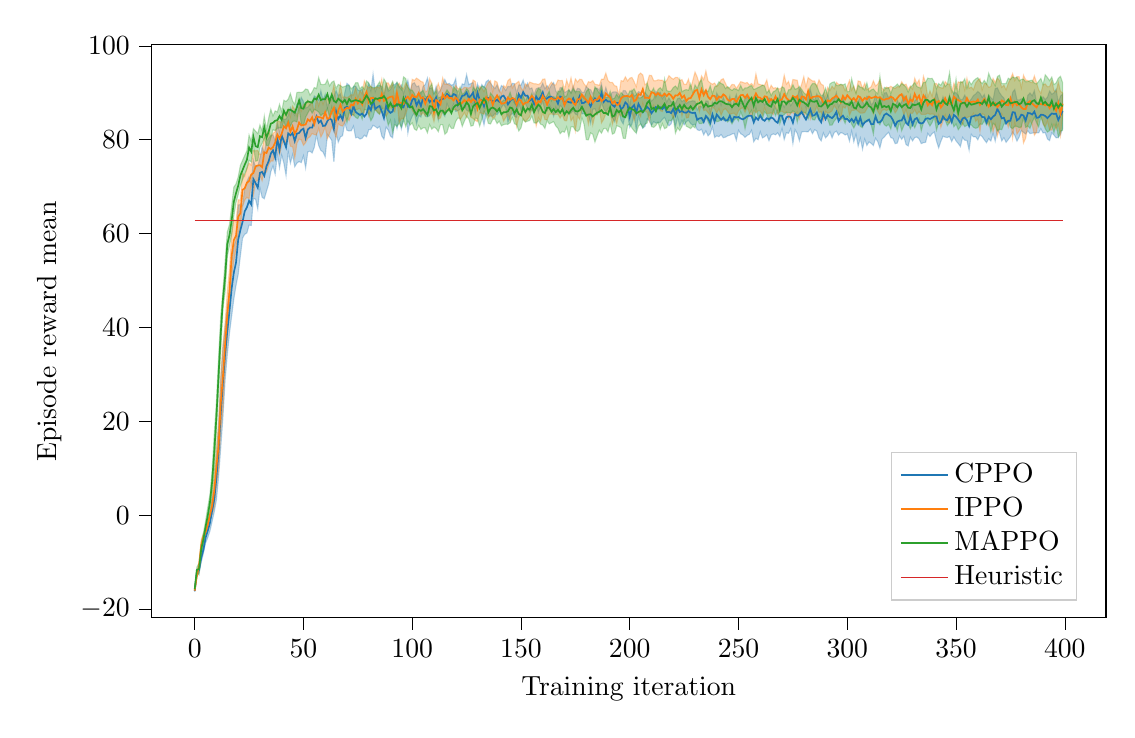
\begin{tikzpicture}

\definecolor{crimson2143940}{RGB}{214,39,40}
\definecolor{darkgray176}{RGB}{176,176,176}
\definecolor{darkorange25512714}{RGB}{255,127,14}
\definecolor{forestgreen4416044}{RGB}{44,160,44}
\definecolor{lightgray204}{RGB}{204,204,204}
\definecolor{steelblue31119180}{RGB}{31,119,180}

\begin{axis}[
scale only axis=true,
width=\linewidth,
height=0.6\linewidth,
legend cell align={left},
legend style={
  fill opacity=0.8,
  draw opacity=1,
  text opacity=1,
  at={(0.97,0.03)},
  anchor=south east,
  draw=lightgray204
},
tick align=outside,
tick pos=left,
x grid style={darkgray176},
xlabel={Training iteration},
xmin=-19.95, xmax=418.95,
xtick style={color=black},
y grid style={darkgray176},
ylabel={Episode reward mean},
ymin=-21.8327154701407, ymax=100.188574603542,
ytick style={color=black}
]
\path [draw=steelblue31119180, fill=steelblue31119180, opacity=0.3]
(axis cs:0,-16.2862931940642)
--(axis cs:0,-15.968408736142)
--(axis cs:1,-11.702821955418)
--(axis cs:2,-11.0590771261434)
--(axis cs:3,-8.12377208623723)
--(axis cs:4,-6.61248068061693)
--(axis cs:5,-3.75622020569895)
--(axis cs:6,-1.87278455018623)
--(axis cs:7,0.0290923770719052)
--(axis cs:8,3.16185307868872)
--(axis cs:9,5.98866758934751)
--(axis cs:10,12.7718323771824)
--(axis cs:11,19.3381277137193)
--(axis cs:12,29.1065013090648)
--(axis cs:13,35.6500169616804)
--(axis cs:14,40.0666622124047)
--(axis cs:15,44.3104675316586)
--(axis cs:16,48.3437049416532)
--(axis cs:17,54.1957222096751)
--(axis cs:18,57.3027466123719)
--(axis cs:19,58.686976921017)
--(axis cs:20,66.0801563264932)
--(axis cs:21,66.1806836268173)
--(axis cs:22,65.9782600345654)
--(axis cs:23,69.5915299884706)
--(axis cs:24,71.0833495271369)
--(axis cs:25,72.1416888774855)
--(axis cs:26,70.6793005599203)
--(axis cs:27,75.7038432732124)
--(axis cs:28,74.1447519307205)
--(axis cs:29,74.288276911467)
--(axis cs:30,76.1080437316788)
--(axis cs:31,78.5317958039233)
--(axis cs:32,77.1481926746895)
--(axis cs:33,79.7007796939044)
--(axis cs:34,80.2622744143087)
--(axis cs:35,80.8886600501889)
--(axis cs:36,81.0435026836339)
--(axis cs:37,79.717758887289)
--(axis cs:38,83.6181827877015)
--(axis cs:39,81.6392213706149)
--(axis cs:40,85.0656684198949)
--(axis cs:41,84.2949066599948)
--(axis cs:42,84.4103780653806)
--(axis cs:43,85.1479515898758)
--(axis cs:44,86.8689962944323)
--(axis cs:45,85.9943666440974)
--(axis cs:46,85.1933669578841)
--(axis cs:47,87.5707718089012)
--(axis cs:48,87.5188402577769)
--(axis cs:49,89.0276177930114)
--(axis cs:50,88.114535103341)
--(axis cs:51,86.7391749486798)
--(axis cs:52,86.9394150973522)
--(axis cs:53,87.6005017981364)
--(axis cs:54,87.95246114337)
--(axis cs:55,89.3366953209141)
--(axis cs:56,88.9307471538085)
--(axis cs:57,88.4607771552176)
--(axis cs:58,90.4452086664624)
--(axis cs:59,88.4553904712792)
--(axis cs:60,89.6606285350171)
--(axis cs:61,86.7726877134143)
--(axis cs:62,88.5824092936182)
--(axis cs:63,88.4800353473869)
--(axis cs:64,89.2372488098477)
--(axis cs:65,90.4851989123866)
--(axis cs:66,89.2843334715132)
--(axis cs:67,89.7950047920034)
--(axis cs:68,87.6372129662406)
--(axis cs:69,90.0149887375094)
--(axis cs:70,91.9930525591444)
--(axis cs:71,91.6250665378812)
--(axis cs:72,89.1232694507292)
--(axis cs:73,91.3375419645678)
--(axis cs:74,91.4196356177228)
--(axis cs:75,90.5873907673702)
--(axis cs:76,90.402644221073)
--(axis cs:77,90.8146626168286)
--(axis cs:78,88.9339953624741)
--(axis cs:79,90.4276210901006)
--(axis cs:80,92.000805749516)
--(axis cs:81,90.3532323762117)
--(axis cs:82,93.9804910517296)
--(axis cs:83,90.2382064584596)
--(axis cs:84,91.4479723194961)
--(axis cs:85,91.5656321097451)
--(axis cs:86,91.3025732582902)
--(axis cs:87,89.1451349899654)
--(axis cs:88,91.7876055199182)
--(axis cs:89,90.3346729907888)
--(axis cs:90,90.6896790380875)
--(axis cs:91,91.6368366452934)
--(axis cs:92,91.7585214221049)
--(axis cs:93,92.1710928240629)
--(axis cs:94,91.0725143332173)
--(axis cs:95,91.6717645405137)
--(axis cs:96,89.8071528335018)
--(axis cs:97,91.3028867954517)
--(axis cs:98,92.6499453479602)
--(axis cs:99,90.1939293176761)
--(axis cs:100,91.8553978809059)
--(axis cs:101,92.1284043559636)
--(axis cs:102,91.2861444426792)
--(axis cs:103,91.462123359958)
--(axis cs:104,89.5274222169159)
--(axis cs:105,91.3325108692303)
--(axis cs:106,91.74693058225)
--(axis cs:107,93.1270995150446)
--(axis cs:108,90.8859064916139)
--(axis cs:109,91.0441873042452)
--(axis cs:110,89.7473026338945)
--(axis cs:111,91.4204360806302)
--(axis cs:112,89.8956048649963)
--(axis cs:113,90.6056796190071)
--(axis cs:114,91.7017823136893)
--(axis cs:115,92.8287752694269)
--(axis cs:116,91.781703004611)
--(axis cs:117,92.0095622514726)
--(axis cs:118,91.5841119684011)
--(axis cs:119,91.8035397131707)
--(axis cs:120,93.0149847629385)
--(axis cs:121,88.6925035974304)
--(axis cs:122,90.3737342521355)
--(axis cs:123,91.8843081006012)
--(axis cs:124,91.74515433437)
--(axis cs:125,93.8750092610041)
--(axis cs:126,91.7211377677672)
--(axis cs:127,91.9503748712913)
--(axis cs:128,92.1846863021083)
--(axis cs:129,90.1448224235479)
--(axis cs:130,91.9196713607572)
--(axis cs:131,90.5774144854137)
--(axis cs:132,91.7557354362143)
--(axis cs:133,91.0979641803796)
--(axis cs:134,92.3434714008154)
--(axis cs:135,92.7097819043414)
--(axis cs:136,92.0165395274117)
--(axis cs:137,91.4194881661906)
--(axis cs:138,90.8520252995207)
--(axis cs:139,91.6852004207279)
--(axis cs:140,90.2875012057934)
--(axis cs:141,91.5410824934515)
--(axis cs:142,91.2021180247326)
--(axis cs:143,90.4651132015578)
--(axis cs:144,91.3604082222943)
--(axis cs:145,91.2743750452838)
--(axis cs:146,92.0077939329173)
--(axis cs:147,91.9235968762261)
--(axis cs:148,89.9801126589688)
--(axis cs:149,91.6650455512212)
--(axis cs:150,91.6106271546656)
--(axis cs:151,92.6964808803382)
--(axis cs:152,91.0266733214907)
--(axis cs:153,92.0263757621156)
--(axis cs:154,90.8087246690671)
--(axis cs:155,91.0408038741279)
--(axis cs:156,89.5750888231321)
--(axis cs:157,90.8649866297162)
--(axis cs:158,91.0624370189773)
--(axis cs:159,91.069942825808)
--(axis cs:160,92.0346495506103)
--(axis cs:161,90.8448278268967)
--(axis cs:162,91.5345215051123)
--(axis cs:163,90.8107631233343)
--(axis cs:164,91.6553690809061)
--(axis cs:165,92.1812320466437)
--(axis cs:166,90.3871485861159)
--(axis cs:167,89.6414882467628)
--(axis cs:168,91.0745389728904)
--(axis cs:169,91.046579135177)
--(axis cs:170,90.0497003314087)
--(axis cs:171,90.2674561524643)
--(axis cs:172,90.6346248602168)
--(axis cs:173,90.0599213051462)
--(axis cs:174,91.4368750168488)
--(axis cs:175,90.0169269214065)
--(axis cs:176,90.9493749207047)
--(axis cs:177,90.8206818453343)
--(axis cs:178,90.0996089693814)
--(axis cs:179,90.0800513883038)
--(axis cs:180,91.3842614452525)
--(axis cs:181,90.8044547698126)
--(axis cs:182,90.6586695354585)
--(axis cs:183,89.7489917626505)
--(axis cs:184,90.9689957691699)
--(axis cs:185,90.9883185241347)
--(axis cs:186,90.5655879702711)
--(axis cs:187,91.9348948331)
--(axis cs:188,89.4706497310426)
--(axis cs:189,91.1277556803406)
--(axis cs:190,89.6290711516982)
--(axis cs:191,89.3786686711719)
--(axis cs:192,90.1359779186586)
--(axis cs:193,90.188877110889)
--(axis cs:194,90.1444510658714)
--(axis cs:195,89.6808201104582)
--(axis cs:196,88.7797691830024)
--(axis cs:197,90.4779577568574)
--(axis cs:198,90.4193651028582)
--(axis cs:199,89.6383944739802)
--(axis cs:200,87.0783133158824)
--(axis cs:201,90.4001974083137)
--(axis cs:202,89.2776099294061)
--(axis cs:203,89.571056095886)
--(axis cs:204,90.243983852399)
--(axis cs:205,90.062040505061)
--(axis cs:206,89.2671331955733)
--(axis cs:207,90.0459558777615)
--(axis cs:208,89.4774501043375)
--(axis cs:209,89.0928581174982)
--(axis cs:210,88.20172167294)
--(axis cs:211,88.6709761304754)
--(axis cs:212,90.3621913036567)
--(axis cs:213,89.6750083656268)
--(axis cs:214,90.0866704531833)
--(axis cs:215,88.7528691627803)
--(axis cs:216,89.5436015780372)
--(axis cs:217,87.9697114883759)
--(axis cs:218,88.9199877729992)
--(axis cs:219,88.0069501247862)
--(axis cs:220,88.2191079625981)
--(axis cs:221,87.6939515967129)
--(axis cs:222,88.7560016941201)
--(axis cs:223,88.8924770818514)
--(axis cs:224,88.0970973230051)
--(axis cs:225,88.464229436086)
--(axis cs:226,87.6592404351464)
--(axis cs:227,88.076897979862)
--(axis cs:228,88.1345881084991)
--(axis cs:229,88.2863553415713)
--(axis cs:230,88.2050959452493)
--(axis cs:231,86.3365565889753)
--(axis cs:232,87.1214019686783)
--(axis cs:233,87.0518750330447)
--(axis cs:234,86.5423415102776)
--(axis cs:235,88.2454731869706)
--(axis cs:236,88.2262931948201)
--(axis cs:237,85.916579158591)
--(axis cs:238,88.009468533231)
--(axis cs:239,87.1721068272638)
--(axis cs:240,89.9268998339944)
--(axis cs:241,89.0014369840408)
--(axis cs:242,87.3562893564928)
--(axis cs:243,89.0728775240446)
--(axis cs:244,87.586106685492)
--(axis cs:245,87.5149494807945)
--(axis cs:246,89.2556955550671)
--(axis cs:247,86.6819064013915)
--(axis cs:248,88.4076377451705)
--(axis cs:249,89.6369689343841)
--(axis cs:250,87.6523509470616)
--(axis cs:251,87.7647016468064)
--(axis cs:252,87.6373915050471)
--(axis cs:253,88.7414523988919)
--(axis cs:254,89.0436823083944)
--(axis cs:255,89.0708994087813)
--(axis cs:256,88.1845347129808)
--(axis cs:257,87.8261254737193)
--(axis cs:258,89.1796619470833)
--(axis cs:259,88.4580995343351)
--(axis cs:260,88.5450388331833)
--(axis cs:261,88.2292755060272)
--(axis cs:262,87.4289659301892)
--(axis cs:263,88.0863878127174)
--(axis cs:264,88.9093344503492)
--(axis cs:265,88.4823359194127)
--(axis cs:266,87.7573583125483)
--(axis cs:267,86.8072266405151)
--(axis cs:268,85.7260765543567)
--(axis cs:269,89.6754256785033)
--(axis cs:270,87.8286209948182)
--(axis cs:271,86.8876028035842)
--(axis cs:272,88.0511495803956)
--(axis cs:273,88.5499351188221)
--(axis cs:274,87.2507185826735)
--(axis cs:275,88.0393562088739)
--(axis cs:276,88.7771714007702)
--(axis cs:277,88.8607053769491)
--(axis cs:278,90.9202686690736)
--(axis cs:279,90.241951899273)
--(axis cs:280,88.4214486117012)
--(axis cs:281,86.9020169410228)
--(axis cs:282,89.1148947006747)
--(axis cs:283,90.6906534422817)
--(axis cs:284,88.9017388272973)
--(axis cs:285,88.3578185734965)
--(axis cs:286,89.7436690034605)
--(axis cs:287,88.5466946719136)
--(axis cs:288,87.6797002818906)
--(axis cs:289,89.7786781616027)
--(axis cs:290,88.3322125810169)
--(axis cs:291,89.6453919684348)
--(axis cs:292,87.953006341918)
--(axis cs:293,88.8112901855632)
--(axis cs:294,88.6646194534097)
--(axis cs:295,90.0523966111726)
--(axis cs:296,86.954762239238)
--(axis cs:297,87.8958857733363)
--(axis cs:298,88.8711882363469)
--(axis cs:299,87.7360470110405)
--(axis cs:300,87.6462796589917)
--(axis cs:301,88.0238765794745)
--(axis cs:302,87.0347811704145)
--(axis cs:303,87.9154089629966)
--(axis cs:304,88.2475613005723)
--(axis cs:305,88.2116038602144)
--(axis cs:306,89.0710036141342)
--(axis cs:307,88.1715513381715)
--(axis cs:308,87.1872639073552)
--(axis cs:309,89.2627497118021)
--(axis cs:310,89.0672011839277)
--(axis cs:311,87.3912368222622)
--(axis cs:312,87.9233241932657)
--(axis cs:313,89.5928381733682)
--(axis cs:314,87.7838206027563)
--(axis cs:315,89.1901455324455)
--(axis cs:316,88.3097437583605)
--(axis cs:317,89.9519231513332)
--(axis cs:318,90.013726661387)
--(axis cs:319,88.9076193727822)
--(axis cs:320,89.4513198866328)
--(axis cs:321,88.0739516355773)
--(axis cs:322,86.7507683752125)
--(axis cs:323,88.4152546641977)
--(axis cs:324,87.2940207998919)
--(axis cs:325,88.0893388858266)
--(axis cs:326,89.4216725704752)
--(axis cs:327,88.258986557847)
--(axis cs:328,87.6732934063703)
--(axis cs:329,89.3865449114999)
--(axis cs:330,86.7417982447353)
--(axis cs:331,88.2624756037462)
--(axis cs:332,88.6980392216318)
--(axis cs:333,87.0997623488761)
--(axis cs:334,87.7288400883764)
--(axis cs:335,87.9249094193923)
--(axis cs:336,89.4451592264261)
--(axis cs:337,87.7908934663516)
--(axis cs:338,88.1251780988243)
--(axis cs:339,88.0131134676835)
--(axis cs:340,88.2856888954192)
--(axis cs:341,90.1891950467598)
--(axis cs:342,88.4771654927702)
--(axis cs:343,87.7398074881735)
--(axis cs:344,89.1525166096202)
--(axis cs:345,88.139729557599)
--(axis cs:346,87.7833560342571)
--(axis cs:347,89.5272356980058)
--(axis cs:348,87.9290421839464)
--(axis cs:349,90.0053146631003)
--(axis cs:350,89.9995918136649)
--(axis cs:351,89.3627241294057)
--(axis cs:352,88.5361846923161)
--(axis cs:353,88.5466536021814)
--(axis cs:354,89.5137881326636)
--(axis cs:355,88.3940647156664)
--(axis cs:356,88.0949694578504)
--(axis cs:357,88.6509246622263)
--(axis cs:358,89.3990704959269)
--(axis cs:359,89.7427699328014)
--(axis cs:360,90.2779391027474)
--(axis cs:361,89.8932211398912)
--(axis cs:362,88.994122902939)
--(axis cs:363,89.6274301254706)
--(axis cs:364,87.9993634114478)
--(axis cs:365,89.549409226023)
--(axis cs:366,88.9587175266928)
--(axis cs:367,88.4776678476008)
--(axis cs:368,90.8685416176505)
--(axis cs:369,91.0392450148756)
--(axis cs:370,89.9950307659869)
--(axis cs:371,89.3419642977021)
--(axis cs:372,88.8680710986409)
--(axis cs:373,87.4725863082198)
--(axis cs:374,88.0325820828009)
--(axis cs:375,87.4078524405487)
--(axis cs:376,90.1089565492957)
--(axis cs:377,90.6957860313897)
--(axis cs:378,88.52893666739)
--(axis cs:379,88.437339005328)
--(axis cs:380,88.6908126523507)
--(axis cs:381,88.7418243406737)
--(axis cs:382,86.9305717642858)
--(axis cs:383,89.4550776015775)
--(axis cs:384,89.9531751255518)
--(axis cs:385,89.3561410605461)
--(axis cs:386,90.4576989696229)
--(axis cs:387,87.9043423100088)
--(axis cs:388,87.9888206796096)
--(axis cs:389,88.2824956168278)
--(axis cs:390,89.1366991138199)
--(axis cs:391,88.5559317486818)
--(axis cs:392,89.0290508033629)
--(axis cs:393,90.3700116640024)
--(axis cs:394,89.6841958443924)
--(axis cs:395,89.9550055414026)
--(axis cs:396,90.751052679573)
--(axis cs:397,87.8781202399814)
--(axis cs:398,89.2803171571992)
--(axis cs:399,89.6876447239257)
--(axis cs:399,82.4741176001793)
--(axis cs:399,82.4741176001793)
--(axis cs:398,81.0890186346683)
--(axis cs:397,80.4728553814522)
--(axis cs:396,80.3884743567079)
--(axis cs:395,80.9933379785428)
--(axis cs:394,81.49553131541)
--(axis cs:393,79.8122145893824)
--(axis cs:392,80.1504975719042)
--(axis cs:391,81.5327031609443)
--(axis cs:390,81.4416917825702)
--(axis cs:389,82.3532376735664)
--(axis cs:388,81.4401042070374)
--(axis cs:387,81.443450225769)
--(axis cs:386,81.49180444201)
--(axis cs:385,81.4010357968334)
--(axis cs:384,81.3005738097606)
--(axis cs:383,81.9050077840239)
--(axis cs:382,81.2181826457997)
--(axis cs:381,81.5687312552346)
--(axis cs:380,81.9644771636252)
--(axis cs:379,80.5472039297888)
--(axis cs:378,79.7045052892383)
--(axis cs:377,80.910593292999)
--(axis cs:376,81.6120693141339)
--(axis cs:375,80.6687614956744)
--(axis cs:374,80.034208426405)
--(axis cs:373,79.4421888054514)
--(axis cs:372,80.4393936303494)
--(axis cs:371,79.7370455781125)
--(axis cs:370,81.4158025082637)
--(axis cs:369,82.0595693729596)
--(axis cs:368,79.6949144908727)
--(axis cs:367,81.3535272930587)
--(axis cs:366,79.7197332528541)
--(axis cs:365,80.2295280167244)
--(axis cs:364,79.3761615379047)
--(axis cs:363,79.9675586595441)
--(axis cs:362,80.6862091026797)
--(axis cs:361,81.0162012769075)
--(axis cs:360,79.9817589889867)
--(axis cs:359,80.6407171286228)
--(axis cs:358,80.6046711491738)
--(axis cs:357,81.1736513655097)
--(axis cs:356,77.7682937168528)
--(axis cs:355,79.8565945055663)
--(axis cs:354,79.8913197659918)
--(axis cs:353,80.4838246271781)
--(axis cs:352,78.5358120918197)
--(axis cs:351,79.1945042016341)
--(axis cs:350,79.741850384739)
--(axis cs:349,80.5868905140771)
--(axis cs:348,79.6039308138185)
--(axis cs:347,80.7016036395853)
--(axis cs:346,80.4544455145914)
--(axis cs:345,80.5511053816676)
--(axis cs:344,80.7464768305741)
--(axis cs:343,79.6258434636897)
--(axis cs:342,78.270381788378)
--(axis cs:341,79.7404622873277)
--(axis cs:340,81.6428690653742)
--(axis cs:339,81.3011968753703)
--(axis cs:338,80.68854575388)
--(axis cs:337,81.3447697403391)
--(axis cs:336,79.4291668760837)
--(axis cs:335,79.3663752369147)
--(axis cs:334,79.1757540468742)
--(axis cs:333,80.163039010495)
--(axis cs:332,80.5726399083039)
--(axis cs:331,80.4510485525696)
--(axis cs:330,79.7602979257903)
--(axis cs:329,80.5493163213796)
--(axis cs:328,78.677343389355)
--(axis cs:327,78.9766593215953)
--(axis cs:326,80.7668007856925)
--(axis cs:325,80.0849803983626)
--(axis cs:324,80.832812405695)
--(axis cs:323,79.2909533017495)
--(axis cs:322,79.1591828711934)
--(axis cs:321,80.2753545070691)
--(axis cs:320,80.4455614621472)
--(axis cs:319,81.5739673998975)
--(axis cs:318,81.1447775771264)
--(axis cs:317,80.5830566715905)
--(axis cs:316,80.1539930506659)
--(axis cs:315,78.2259661526001)
--(axis cs:314,79.5878237404213)
--(axis cs:313,80.3138743164622)
--(axis cs:312,78.7543967545503)
--(axis cs:311,79.2194038801161)
--(axis cs:310,79.5361400352756)
--(axis cs:309,78.7854476783956)
--(axis cs:308,80.1359691637388)
--(axis cs:307,77.9932804465414)
--(axis cs:306,80.3438592451664)
--(axis cs:305,78.6290017239375)
--(axis cs:304,81.1676710844136)
--(axis cs:303,79.547469838905)
--(axis cs:302,81.8175881536916)
--(axis cs:301,79.7003174208535)
--(axis cs:300,81.242070283439)
--(axis cs:299,81.0126976106756)
--(axis cs:298,81.363945391624)
--(axis cs:297,81.5117357292621)
--(axis cs:296,80.9796336412458)
--(axis cs:295,81.8202993569176)
--(axis cs:294,81.5293065117862)
--(axis cs:293,80.3874081263212)
--(axis cs:292,81.7277260215534)
--(axis cs:291,80.8518960547177)
--(axis cs:290,80.4024594280215)
--(axis cs:289,81.4535678367881)
--(axis cs:288,79.7529783299841)
--(axis cs:287,80.3912192120036)
--(axis cs:286,81.8530487540913)
--(axis cs:285,82.1215666847886)
--(axis cs:284,81.301484990994)
--(axis cs:283,82.2681138332808)
--(axis cs:282,81.6773165896964)
--(axis cs:281,81.7036749905119)
--(axis cs:280,81.7292769447752)
--(axis cs:279,81.6270025862461)
--(axis cs:278,79.7810951351081)
--(axis cs:277,81.3442618094785)
--(axis cs:276,82.1422294079352)
--(axis cs:275,79.1714060897868)
--(axis cs:274,82.4036948101092)
--(axis cs:273,81.3582774296367)
--(axis cs:272,81.4816571876343)
--(axis cs:271,80.0487895651387)
--(axis cs:270,82.4042797021974)
--(axis cs:269,80.680362552341)
--(axis cs:268,81.468947096067)
--(axis cs:267,81.0376132898825)
--(axis cs:266,81.2473108122769)
--(axis cs:265,81.0073994938266)
--(axis cs:264,79.7914147154611)
--(axis cs:263,81.0660823018335)
--(axis cs:262,80.6202150178174)
--(axis cs:261,80.3833510495299)
--(axis cs:260,81.706700865854)
--(axis cs:259,80.0152147406961)
--(axis cs:258,80.3062144654929)
--(axis cs:257,79.5573464092404)
--(axis cs:256,82.0291158802635)
--(axis cs:255,81.1542067257923)
--(axis cs:254,80.929931901272)
--(axis cs:253,80.4999185873851)
--(axis cs:252,81.016460432192)
--(axis cs:251,81.2714767491681)
--(axis cs:250,82.0101127800362)
--(axis cs:249,79.8745854450797)
--(axis cs:248,81.3433758247401)
--(axis cs:247,81.2100868956593)
--(axis cs:246,80.9687558246391)
--(axis cs:245,80.8260927302892)
--(axis cs:244,80.5409534527447)
--(axis cs:243,80.4174376147355)
--(axis cs:242,81.0952213801443)
--(axis cs:241,80.6362364009242)
--(axis cs:240,80.8176963889357)
--(axis cs:239,80.4787282084334)
--(axis cs:238,82.759457358607)
--(axis cs:237,81.3200914788865)
--(axis cs:236,80.8361513849991)
--(axis cs:235,81.8859410329019)
--(axis cs:234,81.0224198084893)
--(axis cs:233,82.2227149177458)
--(axis cs:232,81.9445745841347)
--(axis cs:231,82.1424361589445)
--(axis cs:230,83.3088051247978)
--(axis cs:229,83.0946015190859)
--(axis cs:228,83.4238064961956)
--(axis cs:227,84.1371817381311)
--(axis cs:226,83.8369172677311)
--(axis cs:225,83.1498067719086)
--(axis cs:224,84.1357271900362)
--(axis cs:223,82.912897473752)
--(axis cs:222,84.8076220053663)
--(axis cs:221,82.7294222400195)
--(axis cs:220,84.8670498940856)
--(axis cs:219,83.3654880883307)
--(axis cs:218,82.9537170098453)
--(axis cs:217,83.7197609876004)
--(axis cs:216,84.7451160537451)
--(axis cs:215,84.3255425455006)
--(axis cs:214,83.7173598505931)
--(axis cs:213,83.6005981399574)
--(axis cs:212,83.5561319294912)
--(axis cs:211,83.8466728550793)
--(axis cs:210,83.0619357925049)
--(axis cs:209,83.9827803697236)
--(axis cs:208,84.4804464088834)
--(axis cs:207,82.847999429838)
--(axis cs:206,82.4643354760507)
--(axis cs:205,83.4575662347789)
--(axis cs:204,85.0130637866763)
--(axis cs:203,81.9244079212031)
--(axis cs:202,85.4724370759178)
--(axis cs:201,83.321114553054)
--(axis cs:200,82.6248500100137)
--(axis cs:199,85.3214368079222)
--(axis cs:198,85.4873772578729)
--(axis cs:197,83.3630665920855)
--(axis cs:196,84.1374030759138)
--(axis cs:195,86.0375509367287)
--(axis cs:194,85.4879821718784)
--(axis cs:193,83.8514500878969)
--(axis cs:192,84.6519800228484)
--(axis cs:191,86.9793943493463)
--(axis cs:190,86.6056029411464)
--(axis cs:189,85.9111458072164)
--(axis cs:188,86.6202083060959)
--(axis cs:187,87.9603631229502)
--(axis cs:186,86.0363753357057)
--(axis cs:185,85.4031467964385)
--(axis cs:184,86.6229678305891)
--(axis cs:183,86.4711235890344)
--(axis cs:182,83.4910704468777)
--(axis cs:181,85.0792250937543)
--(axis cs:180,85.0803646951234)
--(axis cs:179,85.6190801550431)
--(axis cs:178,85.4732919525178)
--(axis cs:177,87.7536047690621)
--(axis cs:176,85.2308588678359)
--(axis cs:175,85.4843316756026)
--(axis cs:174,86.2126373801948)
--(axis cs:173,85.6891122289496)
--(axis cs:172,85.3677261338366)
--(axis cs:171,86.1514441737307)
--(axis cs:170,85.1153846396188)
--(axis cs:169,86.824268444592)
--(axis cs:168,87.3182433203511)
--(axis cs:167,85.7117577429756)
--(axis cs:166,86.9374386032627)
--(axis cs:165,85.0235195491887)
--(axis cs:164,86.6521011691396)
--(axis cs:163,87.4628551394087)
--(axis cs:162,86.1100704046563)
--(axis cs:161,86.2063676459079)
--(axis cs:160,88.1854103267554)
--(axis cs:159,87.143248482792)
--(axis cs:158,85.7965276524038)
--(axis cs:157,87.5501871560789)
--(axis cs:156,85.6254551781425)
--(axis cs:155,86.4273944631997)
--(axis cs:154,85.8198276292428)
--(axis cs:153,86.7599257477867)
--(axis cs:152,87.7025791598496)
--(axis cs:151,87.5873843748488)
--(axis cs:150,86.1949495597205)
--(axis cs:149,87.7300355139854)
--(axis cs:148,84.730658481774)
--(axis cs:147,85.0053289538353)
--(axis cs:146,85.6351781885623)
--(axis cs:145,85.1635569758759)
--(axis cs:144,83.6577594929782)
--(axis cs:143,86.7776965593565)
--(axis cs:142,87.5563277733707)
--(axis cs:141,86.8585639429465)
--(axis cs:140,85.9286839174762)
--(axis cs:139,85.3222421807051)
--(axis cs:138,85.5316552970052)
--(axis cs:137,84.9939158128568)
--(axis cs:136,85.0350687545843)
--(axis cs:135,85.0262824957065)
--(axis cs:134,85.5377909728914)
--(axis cs:133,83.139042045441)
--(axis cs:132,85.0337453720178)
--(axis cs:131,86.4618771532196)
--(axis cs:130,88.1214246784243)
--(axis cs:129,85.4841861705115)
--(axis cs:128,87.8599318466795)
--(axis cs:127,86.8443159141284)
--(axis cs:126,86.0420431548795)
--(axis cs:125,86.2999313223713)
--(axis cs:124,87.1434550768341)
--(axis cs:123,86.8123755912672)
--(axis cs:122,86.4763850215997)
--(axis cs:121,86.1828955601214)
--(axis cs:120,86.0227096983232)
--(axis cs:119,87.6242293609854)
--(axis cs:118,86.5009374104921)
--(axis cs:117,86.5638954556182)
--(axis cs:116,87.7250344851251)
--(axis cs:115,84.9542725422536)
--(axis cs:114,85.6666050530825)
--(axis cs:113,86.4740984452926)
--(axis cs:112,84.1564482500834)
--(axis cs:111,86.550642698618)
--(axis cs:110,86.5328710569646)
--(axis cs:109,85.8959232928372)
--(axis cs:108,85.1300321975659)
--(axis cs:107,84.840043898148)
--(axis cs:106,85.0312518543255)
--(axis cs:105,86.5142350598704)
--(axis cs:104,84.8302232095633)
--(axis cs:103,85.154325922503)
--(axis cs:102,83.3478018995277)
--(axis cs:101,85.7642347281119)
--(axis cs:100,84.9965450799487)
--(axis cs:99,83.8612384230751)
--(axis cs:98,81.389801705258)
--(axis cs:97,86.2313213303445)
--(axis cs:96,83.9420795109679)
--(axis cs:95,82.2742083604221)
--(axis cs:94,84.5208369319035)
--(axis cs:93,82.3491972538573)
--(axis cs:92,84.0948774231916)
--(axis cs:91,80.3953406978783)
--(axis cs:90,80.7515354867428)
--(axis cs:89,82.0696686333899)
--(axis cs:88,82.6986422498903)
--(axis cs:87,80.0936481476911)
--(axis cs:86,80.7853523623709)
--(axis cs:85,82.8317254604839)
--(axis cs:84,82.4372630395583)
--(axis cs:83,82.8151099444901)
--(axis cs:82,83.0756466604416)
--(axis cs:81,82.2118422351405)
--(axis cs:80,82.1117005567115)
--(axis cs:79,80.6276234921767)
--(axis cs:78,80.9498032708726)
--(axis cs:77,80.3280888766363)
--(axis cs:76,80.129229350233)
--(axis cs:75,80.5164987966275)
--(axis cs:74,80.4039976836837)
--(axis cs:73,82.8977323993617)
--(axis cs:72,81.898842145537)
--(axis cs:71,81.8593862233702)
--(axis cs:70,82.0018882166215)
--(axis cs:69,83.5948041784456)
--(axis cs:68,80.8735819679774)
--(axis cs:67,80.5683584606928)
--(axis cs:66,79.4614836170024)
--(axis cs:65,81.5623520722581)
--(axis cs:64,75.2960609856424)
--(axis cs:63,79.8947720797303)
--(axis cs:62,80.5774066178555)
--(axis cs:61,81.1571894007611)
--(axis cs:60,76.3246870274285)
--(axis cs:59,77.3981979788166)
--(axis cs:58,77.7038643007218)
--(axis cs:57,78.7704710402269)
--(axis cs:56,81.0193014006716)
--(axis cs:55,78.4079001070988)
--(axis cs:54,77.181213710764)
--(axis cs:53,77.5698149508798)
--(axis cs:52,77.4059370430046)
--(axis cs:51,73.9755309201375)
--(axis cs:50,76.5800557612436)
--(axis cs:49,75.1182435297247)
--(axis cs:48,75.3445349955417)
--(axis cs:47,75.0268813824267)
--(axis cs:46,74.2418261769477)
--(axis cs:45,76.8204093221553)
--(axis cs:44,75.0042416945528)
--(axis cs:43,77.5222258540748)
--(axis cs:42,72.3620770236845)
--(axis cs:41,75.0201246441665)
--(axis cs:40,76.7708535501183)
--(axis cs:39,74.0056352743737)
--(axis cs:38,76.84038872661)
--(axis cs:37,72.662022571495)
--(axis cs:36,74.4172056261771)
--(axis cs:35,73.1837808991451)
--(axis cs:34,70.5621178980541)
--(axis cs:33,69.0014356923755)
--(axis cs:32,67.4264403417268)
--(axis cs:31,67.7299624799313)
--(axis cs:30,69.756463496664)
--(axis cs:29,65.2508820424005)
--(axis cs:28,67.3459288659859)
--(axis cs:27,67.4888320510364)
--(axis cs:26,61.7436602885063)
--(axis cs:25,61.8154334502154)
--(axis cs:24,60.1360769875991)
--(axis cs:23,59.8696962550151)
--(axis cs:22,59.0388322168367)
--(axis cs:21,55.2285918652006)
--(axis cs:20,51.3078093735057)
--(axis cs:19,48.9667473154102)
--(axis cs:18,46.0907792767341)
--(axis cs:17,42.4501046600053)
--(axis cs:16,38.7593300927406)
--(axis cs:15,34.2284614760886)
--(axis cs:14,28.8252772081933)
--(axis cs:13,21.0287502574664)
--(axis cs:12,14.5375776437771)
--(axis cs:11,8.22077077569275)
--(axis cs:10,3.28704693153968)
--(axis cs:9,0.745301028127113)
--(axis cs:8,-1.33682079905729)
--(axis cs:7,-3.38569534340872)
--(axis cs:6,-4.78645643733235)
--(axis cs:5,-5.90316868248439)
--(axis cs:4,-8.12306387284996)
--(axis cs:3,-10.0194680749446)
--(axis cs:2,-12.3209054115102)
--(axis cs:1,-12.8471549267317)
--(axis cs:0,-16.2862931940642)
--cycle;

\path [draw=darkorange25512714, fill=darkorange25512714, opacity=0.3]
(axis cs:0,-16.0849338992067)
--(axis cs:0,-16.0379561633738)
--(axis cs:1,-12.4455965182257)
--(axis cs:2,-9.91863892022393)
--(axis cs:3,-5.26739136923208)
--(axis cs:4,-3.89624336399987)
--(axis cs:5,-2.87457307579636)
--(axis cs:6,-1.13697169675478)
--(axis cs:7,0.360587449984491)
--(axis cs:8,3.80270936355637)
--(axis cs:9,8.54980753011976)
--(axis cs:10,14.1713163924836)
--(axis cs:11,19.7984265030989)
--(axis cs:12,29.6321547970533)
--(axis cs:13,36.355124171124)
--(axis cs:14,41.0600923393145)
--(axis cs:15,47.588894154589)
--(axis cs:16,52.3956961485945)
--(axis cs:17,59.6961504567382)
--(axis cs:18,62.9970309195112)
--(axis cs:19,62.4398625359228)
--(axis cs:20,67.2053759887316)
--(axis cs:21,67.1734886545218)
--(axis cs:22,72.9586973202637)
--(axis cs:23,72.1710106424374)
--(axis cs:24,73.9016668970525)
--(axis cs:25,75.0401125415571)
--(axis cs:26,74.5556445059477)
--(axis cs:27,77.7232297940117)
--(axis cs:28,77.6269008644304)
--(axis cs:29,77.7111796166586)
--(axis cs:30,76.8121803116771)
--(axis cs:31,77.0686069277673)
--(axis cs:32,81.2193481677005)
--(axis cs:33,81.2287201662987)
--(axis cs:34,82.0412256927036)
--(axis cs:35,80.5342230900424)
--(axis cs:36,81.3805817932212)
--(axis cs:37,81.661888863355)
--(axis cs:38,84.0542541167569)
--(axis cs:39,83.8349360259743)
--(axis cs:40,83.7222147854347)
--(axis cs:41,85.7106223918242)
--(axis cs:42,85.7266738995434)
--(axis cs:43,86.5525613530973)
--(axis cs:44,84.8956680033351)
--(axis cs:45,87.1557643264192)
--(axis cs:46,86.4257992210714)
--(axis cs:47,85.0258045025419)
--(axis cs:48,87.1621708040572)
--(axis cs:49,86.0970043919467)
--(axis cs:50,87.471626087421)
--(axis cs:51,87.0928256850199)
--(axis cs:52,88.3519469723812)
--(axis cs:53,87.2873765411477)
--(axis cs:54,88.22341600674)
--(axis cs:55,85.5451424468783)
--(axis cs:56,88.8720932786079)
--(axis cs:57,87.2290835754411)
--(axis cs:58,88.9142776961609)
--(axis cs:59,87.5504562618198)
--(axis cs:60,88.9678375090768)
--(axis cs:61,88.6887463589196)
--(axis cs:62,87.90022600666)
--(axis cs:63,89.285671678259)
--(axis cs:64,91.6907775970254)
--(axis cs:65,88.0339452266905)
--(axis cs:66,89.1523852959499)
--(axis cs:67,91.8145168281741)
--(axis cs:68,89.0395970073847)
--(axis cs:69,89.1463478345986)
--(axis cs:70,88.9426763461029)
--(axis cs:71,89.213324805864)
--(axis cs:72,89.5913837446019)
--(axis cs:73,89.514743355442)
--(axis cs:74,91.0632532037947)
--(axis cs:75,88.9798061541989)
--(axis cs:76,90.4604928104238)
--(axis cs:77,89.7208202331163)
--(axis cs:78,92.533072351769)
--(axis cs:79,91.5032147181569)
--(axis cs:80,91.0298933043464)
--(axis cs:81,91.4100940259737)
--(axis cs:82,90.7904507491117)
--(axis cs:83,91.0228628806496)
--(axis cs:84,91.248973297733)
--(axis cs:85,90.9893534964694)
--(axis cs:86,92.888687228913)
--(axis cs:87,89.8114062357731)
--(axis cs:88,92.0628205822338)
--(axis cs:89,92.0873942296284)
--(axis cs:90,91.1899797536304)
--(axis cs:91,92.118919794363)
--(axis cs:92,88.5883764912344)
--(axis cs:93,91.445273753797)
--(axis cs:94,92.0474616481872)
--(axis cs:95,91.185805563939)
--(axis cs:96,90.8069659770159)
--(axis cs:97,92.0635131310839)
--(axis cs:98,91.4257261705041)
--(axis cs:99,89.4741236007324)
--(axis cs:100,92.8682112432128)
--(axis cs:101,92.6205203164488)
--(axis cs:102,93.1105507358832)
--(axis cs:103,92.7947770156672)
--(axis cs:104,92.4238930012394)
--(axis cs:105,92.2457684511436)
--(axis cs:106,90.1817755186446)
--(axis cs:107,90.4036822092132)
--(axis cs:108,92.9896203430995)
--(axis cs:109,91.9938346074722)
--(axis cs:110,87.6946838740713)
--(axis cs:111,90.7038048487459)
--(axis cs:112,91.9828776638643)
--(axis cs:113,90.4785188238543)
--(axis cs:114,93.1657602974118)
--(axis cs:115,91.802510433926)
--(axis cs:116,91.9084493805204)
--(axis cs:117,91.649311839249)
--(axis cs:118,91.3283101891254)
--(axis cs:119,90.3681020596323)
--(axis cs:120,91.5634157287038)
--(axis cs:121,90.8632739787143)
--(axis cs:122,90.8255921406708)
--(axis cs:123,90.722870036386)
--(axis cs:124,91.159101945886)
--(axis cs:125,91.09556043757)
--(axis cs:126,90.9908322012433)
--(axis cs:127,91.245773257288)
--(axis cs:128,92.7087668610487)
--(axis cs:129,92.3843581299507)
--(axis cs:130,89.328093703664)
--(axis cs:131,91.3452144628966)
--(axis cs:132,90.990073833104)
--(axis cs:133,90.2705056479027)
--(axis cs:134,91.2453800656641)
--(axis cs:135,92.2046398295551)
--(axis cs:136,92.5724684600622)
--(axis cs:137,90.1908331709587)
--(axis cs:138,92.5286395839184)
--(axis cs:139,92.2511916621678)
--(axis cs:140,90.6751742438256)
--(axis cs:141,89.7774264824595)
--(axis cs:142,91.5425289678355)
--(axis cs:143,91.1384716525279)
--(axis cs:144,92.5723934581416)
--(axis cs:145,92.9822245768108)
--(axis cs:146,91.0031239892177)
--(axis cs:147,91.7750930368359)
--(axis cs:148,92.0697897807159)
--(axis cs:149,92.4383733085646)
--(axis cs:150,91.039564898886)
--(axis cs:151,90.4453684352051)
--(axis cs:152,91.9424789187266)
--(axis cs:153,91.4211804856514)
--(axis cs:154,92.2698999258064)
--(axis cs:155,92.0997541144022)
--(axis cs:156,91.9112320264158)
--(axis cs:157,91.9062106081214)
--(axis cs:158,91.7403587112829)
--(axis cs:159,92.0600114673293)
--(axis cs:160,92.8784939810236)
--(axis cs:161,92.9446742639141)
--(axis cs:162,90.6709520478403)
--(axis cs:163,91.6433966810968)
--(axis cs:164,92.259414495955)
--(axis cs:165,91.7054324251814)
--(axis cs:166,91.6508629416624)
--(axis cs:167,92.7060208397879)
--(axis cs:168,92.5680475833173)
--(axis cs:169,92.6347333532985)
--(axis cs:170,90.6033472383031)
--(axis cs:171,92.713858005977)
--(axis cs:172,91.2866911426974)
--(axis cs:173,93.1712161690887)
--(axis cs:174,90.8908727733138)
--(axis cs:175,92.9509867976287)
--(axis cs:176,92.2875998681721)
--(axis cs:177,92.8776847899)
--(axis cs:178,92.807499770418)
--(axis cs:179,91.8839705486281)
--(axis cs:180,91.3305320345385)
--(axis cs:181,92.3525972304988)
--(axis cs:182,92.2238101715968)
--(axis cs:183,92.5989517063568)
--(axis cs:184,91.8063981059542)
--(axis cs:185,91.7139671438744)
--(axis cs:186,91.5898386731349)
--(axis cs:187,92.8985540462475)
--(axis cs:188,92.86832360695)
--(axis cs:189,94.1892536695465)
--(axis cs:190,92.6243999743339)
--(axis cs:191,92.1922225467937)
--(axis cs:192,92.21469176469)
--(axis cs:193,91.5058676561315)
--(axis cs:194,91.3771877270819)
--(axis cs:195,89.4526012155585)
--(axis cs:196,92.592022622012)
--(axis cs:197,92.4515452845715)
--(axis cs:198,93.3918900482891)
--(axis cs:199,92.5070712544566)
--(axis cs:200,93.1036470341545)
--(axis cs:201,93.2738326310822)
--(axis cs:202,92.3676005289953)
--(axis cs:203,91.2781253564842)
--(axis cs:204,93.7297191523569)
--(axis cs:205,94.1882793000258)
--(axis cs:206,93.7817587269401)
--(axis cs:207,91.6825705861117)
--(axis cs:208,92.027331841668)
--(axis cs:209,93.720000488504)
--(axis cs:210,93.6913393930097)
--(axis cs:211,92.5696602271104)
--(axis cs:212,92.5443572880464)
--(axis cs:213,92.7670783896571)
--(axis cs:214,92.6767849410393)
--(axis cs:215,92.6610056567716)
--(axis cs:216,92.2241234076525)
--(axis cs:217,92.6044165250245)
--(axis cs:218,93.6366133263694)
--(axis cs:219,93.198626086135)
--(axis cs:220,92.8796945499082)
--(axis cs:221,93.2599444155648)
--(axis cs:222,93.2772851981774)
--(axis cs:223,92.569123175708)
--(axis cs:224,92.8083469214829)
--(axis cs:225,91.7735264507237)
--(axis cs:226,91.8179724837397)
--(axis cs:227,92.9057247703878)
--(axis cs:228,90.8863434135796)
--(axis cs:229,92.6362272944631)
--(axis cs:230,94.4042082459614)
--(axis cs:231,93.364156749573)
--(axis cs:232,91.8538820424526)
--(axis cs:233,93.5843773999948)
--(axis cs:234,92.7732752823337)
--(axis cs:235,94.6421523274658)
--(axis cs:236,92.4988868039714)
--(axis cs:237,92.0964807714959)
--(axis cs:238,91.8173751803012)
--(axis cs:239,92.0713013907184)
--(axis cs:240,91.3039598940256)
--(axis cs:241,91.8063266054102)
--(axis cs:242,92.7662989429663)
--(axis cs:243,93.0004383796452)
--(axis cs:244,91.9950565115733)
--(axis cs:245,91.0292522090287)
--(axis cs:246,91.1261274954604)
--(axis cs:247,91.7675129273026)
--(axis cs:248,91.7355419202012)
--(axis cs:249,90.9293243431851)
--(axis cs:250,91.6013776927585)
--(axis cs:251,92.3616476293637)
--(axis cs:252,92.2215380960149)
--(axis cs:253,92.0336062197524)
--(axis cs:254,92.1921278334759)
--(axis cs:255,91.6402998081019)
--(axis cs:256,91.9739617342949)
--(axis cs:257,91.3867695689369)
--(axis cs:258,94.0107763490633)
--(axis cs:259,91.8819871007352)
--(axis cs:260,91.754650198796)
--(axis cs:261,91.6025259417983)
--(axis cs:262,91.6625521393616)
--(axis cs:263,92.7236485275278)
--(axis cs:264,90.4632523763267)
--(axis cs:265,91.5892682467428)
--(axis cs:266,90.9562316805246)
--(axis cs:267,91.0725527499834)
--(axis cs:268,90.8975167684925)
--(axis cs:269,90.811536160411)
--(axis cs:270,91.1636715257163)
--(axis cs:271,93.727869968472)
--(axis cs:272,91.8176032256629)
--(axis cs:273,92.4111780493673)
--(axis cs:274,90.8534822914138)
--(axis cs:275,92.8264638072308)
--(axis cs:276,92.7396127874989)
--(axis cs:277,92.6587254817174)
--(axis cs:278,90.3567753106472)
--(axis cs:279,91.7885327509914)
--(axis cs:280,93.4161995050303)
--(axis cs:281,91.2050818165459)
--(axis cs:282,93.2430199281452)
--(axis cs:283,92.8200182584194)
--(axis cs:284,92.5047549103973)
--(axis cs:285,92.4972263192117)
--(axis cs:286,91.3373844968622)
--(axis cs:287,92.7245770936988)
--(axis cs:288,91.8002137114915)
--(axis cs:289,91.5708695342015)
--(axis cs:290,89.2482516647485)
--(axis cs:291,91.1493237775609)
--(axis cs:292,90.4803198399593)
--(axis cs:293,91.40344752575)
--(axis cs:294,90.8457859502968)
--(axis cs:295,92.2092541220007)
--(axis cs:296,91.7932271820673)
--(axis cs:297,91.7034671609565)
--(axis cs:298,91.5908002234547)
--(axis cs:299,90.4483168974214)
--(axis cs:300,91.3783098066357)
--(axis cs:301,92.6209776107141)
--(axis cs:302,90.5582095467967)
--(axis cs:303,91.4769680916462)
--(axis cs:304,89.9826851284222)
--(axis cs:305,92.5239707089313)
--(axis cs:306,92.3583937027835)
--(axis cs:307,90.8909429573076)
--(axis cs:308,92.0168321786963)
--(axis cs:309,90.6037556786644)
--(axis cs:310,90.9410398517758)
--(axis cs:311,91.2866578404907)
--(axis cs:312,92.5391725439331)
--(axis cs:313,91.449203601229)
--(axis cs:314,91.809823131311)
--(axis cs:315,92.7728085794201)
--(axis cs:316,90.9360290224473)
--(axis cs:317,90.5234006283555)
--(axis cs:318,91.2162489215438)
--(axis cs:319,91.0181765005425)
--(axis cs:320,91.3821079051986)
--(axis cs:321,91.0879361916641)
--(axis cs:322,90.9008345010481)
--(axis cs:323,91.3305925974231)
--(axis cs:324,91.2143395406607)
--(axis cs:325,92.3418212820921)
--(axis cs:326,91.5876063242611)
--(axis cs:327,91.8389259399308)
--(axis cs:328,90.732770087767)
--(axis cs:329,91.4271124967896)
--(axis cs:330,90.7553945912883)
--(axis cs:331,93.0933763467001)
--(axis cs:332,91.9296465153503)
--(axis cs:333,92.7536270083987)
--(axis cs:334,90.0788297013302)
--(axis cs:335,93.5190825394906)
--(axis cs:336,92.1606752660765)
--(axis cs:337,88.9968020512464)
--(axis cs:338,90.4125999825807)
--(axis cs:339,89.2373379664445)
--(axis cs:340,91.9175105316501)
--(axis cs:341,91.9673051776872)
--(axis cs:342,91.2674090313234)
--(axis cs:343,91.0671495313939)
--(axis cs:344,90.9658404994992)
--(axis cs:345,92.3918910483918)
--(axis cs:346,91.8370760986755)
--(axis cs:347,91.8631800742371)
--(axis cs:348,90.0829033420354)
--(axis cs:349,92.0413237145887)
--(axis cs:350,90.8867635152987)
--(axis cs:351,92.3160591800684)
--(axis cs:352,92.1365930543447)
--(axis cs:353,92.3628969089862)
--(axis cs:354,90.5515010082001)
--(axis cs:355,93.0768746276334)
--(axis cs:356,90.9464199290007)
--(axis cs:357,91.2029769830886)
--(axis cs:358,90.6548539474187)
--(axis cs:359,92.0477486548062)
--(axis cs:360,92.6898940545252)
--(axis cs:361,93.0184254378858)
--(axis cs:362,90.593844811926)
--(axis cs:363,92.0266646143398)
--(axis cs:364,91.9297648097588)
--(axis cs:365,91.1454544704343)
--(axis cs:366,91.3498029925544)
--(axis cs:367,93.0628364048747)
--(axis cs:368,92.2032487253428)
--(axis cs:369,93.1320210995291)
--(axis cs:370,92.6042565259812)
--(axis cs:371,91.1612223784387)
--(axis cs:372,91.6116589312702)
--(axis cs:373,90.6087452817079)
--(axis cs:374,92.0321949483393)
--(axis cs:375,92.9408330460759)
--(axis cs:376,94.08208196567)
--(axis cs:377,92.5838593177737)
--(axis cs:378,93.4543504112905)
--(axis cs:379,93.4004679561775)
--(axis cs:380,91.0508521035026)
--(axis cs:381,93.7391467237595)
--(axis cs:382,92.7419220309045)
--(axis cs:383,92.6098927114761)
--(axis cs:384,92.2914872192497)
--(axis cs:385,92.1362894878919)
--(axis cs:386,93.5875537230425)
--(axis cs:387,92.1678597726096)
--(axis cs:388,90.6003125968976)
--(axis cs:389,89.8506104557729)
--(axis cs:390,91.753818070889)
--(axis cs:391,91.8692604121944)
--(axis cs:392,91.2763879899184)
--(axis cs:393,91.3176252253983)
--(axis cs:394,92.5645760050414)
--(axis cs:395,90.5005704550356)
--(axis cs:396,90.1533403060953)
--(axis cs:397,92.3152552980429)
--(axis cs:398,90.297358992238)
--(axis cs:399,90.0073508556631)
--(axis cs:399,85.3436634864059)
--(axis cs:399,85.3436634864059)
--(axis cs:398,80.8413244258695)
--(axis cs:397,83.2845652822319)
--(axis cs:396,82.1625493015554)
--(axis cs:395,83.2818352535923)
--(axis cs:394,82.0465385135666)
--(axis cs:393,82.0919716394941)
--(axis cs:392,84.0022533816413)
--(axis cs:391,82.7390685373206)
--(axis cs:390,83.3423500657812)
--(axis cs:389,85.2523439368217)
--(axis cs:388,85.0084104645492)
--(axis cs:387,81.6243026414673)
--(axis cs:386,80.9510768505482)
--(axis cs:385,83.2342275955859)
--(axis cs:384,84.1392698477849)
--(axis cs:383,83.0836154385976)
--(axis cs:382,80.3202525432424)
--(axis cs:381,79.293812463214)
--(axis cs:380,82.7348508046633)
--(axis cs:379,81.8709660370133)
--(axis cs:378,81.1837846757985)
--(axis cs:377,83.6401067766021)
--(axis cs:376,80.3458493826639)
--(axis cs:375,84.7295409884742)
--(axis cs:374,82.6706461654926)
--(axis cs:373,84.1234671644013)
--(axis cs:372,84.5842741093358)
--(axis cs:371,85.5443141342084)
--(axis cs:370,82.3850513046274)
--(axis cs:369,80.75448236751)
--(axis cs:368,83.321252361414)
--(axis cs:367,81.6934620766427)
--(axis cs:366,84.3675432229323)
--(axis cs:365,82.9580866873187)
--(axis cs:364,83.9022310788513)
--(axis cs:363,85.3256099795426)
--(axis cs:362,85.5461559155689)
--(axis cs:361,81.7775424444908)
--(axis cs:360,84.4036658719592)
--(axis cs:359,83.9130395240239)
--(axis cs:358,85.6123035748549)
--(axis cs:357,84.8935968310404)
--(axis cs:356,84.9144963058351)
--(axis cs:355,84.6454910054949)
--(axis cs:354,84.902184897846)
--(axis cs:353,83.1710380732355)
--(axis cs:352,84.2843998969275)
--(axis cs:351,84.5152961847305)
--(axis cs:350,86.4830190905328)
--(axis cs:349,86.2582029717294)
--(axis cs:348,85.0660452150546)
--(axis cs:347,83.5636574438308)
--(axis cs:346,83.7029662420437)
--(axis cs:345,85.2788571190904)
--(axis cs:344,83.9417735599777)
--(axis cs:343,82.6200057356373)
--(axis cs:342,85.2032023503121)
--(axis cs:341,83.8714050094269)
--(axis cs:340,85.3937558991409)
--(axis cs:339,85.4850425792689)
--(axis cs:338,85.4111217980349)
--(axis cs:337,85.6516588321788)
--(axis cs:336,85.38045681936)
--(axis cs:335,85.4043291378713)
--(axis cs:334,85.3927625338658)
--(axis cs:333,86.0116237615951)
--(axis cs:332,85.3871331397465)
--(axis cs:331,86.4124684083049)
--(axis cs:330,85.5968293525393)
--(axis cs:329,85.6805216386883)
--(axis cs:328,84.5186061434904)
--(axis cs:327,86.4565993212184)
--(axis cs:326,85.2088284982953)
--(axis cs:325,87.0376781866958)
--(axis cs:324,87.6792459358165)
--(axis cs:323,86.4056946289926)
--(axis cs:322,85.6957664856023)
--(axis cs:321,86.8035865493842)
--(axis cs:320,86.8662252079108)
--(axis cs:319,86.4693856378908)
--(axis cs:318,86.2058266836171)
--(axis cs:317,86.4338945898939)
--(axis cs:316,86.2473515308938)
--(axis cs:315,85.2845779927592)
--(axis cs:314,86.0760904394188)
--(axis cs:313,86.9315424810944)
--(axis cs:312,85.4528844941833)
--(axis cs:311,86.4395513717363)
--(axis cs:310,87.418207534345)
--(axis cs:309,86.5761820523067)
--(axis cs:308,85.7760278653908)
--(axis cs:307,85.6506697514412)
--(axis cs:306,85.6607355242018)
--(axis cs:305,86.0531491457489)
--(axis cs:304,86.4624283227613)
--(axis cs:303,86.2528858351801)
--(axis cs:302,86.2531464073464)
--(axis cs:301,85.217480283272)
--(axis cs:300,87.6079190330447)
--(axis cs:299,86.7168163722889)
--(axis cs:298,87.0456969369538)
--(axis cs:297,84.1867634253433)
--(axis cs:296,85.7275139174524)
--(axis cs:295,86.5751721637316)
--(axis cs:294,87.2650410523723)
--(axis cs:293,86.1242841802975)
--(axis cs:292,85.8225825298043)
--(axis cs:291,85.6128867897507)
--(axis cs:290,86.0433676501928)
--(axis cs:289,84.1157186951122)
--(axis cs:288,85.955634000026)
--(axis cs:287,85.7961839837311)
--(axis cs:286,87.1691709468211)
--(axis cs:285,85.8288362129375)
--(axis cs:284,85.6659270679293)
--(axis cs:283,84.3757859712537)
--(axis cs:282,87.5129307013584)
--(axis cs:281,85.8324856222359)
--(axis cs:280,84.8994580811011)
--(axis cs:279,86.5992008919913)
--(axis cs:278,84.4737500054696)
--(axis cs:277,85.9354665255501)
--(axis cs:276,85.2007745222814)
--(axis cs:275,85.7702796616526)
--(axis cs:274,85.6578353916299)
--(axis cs:273,84.4423853316724)
--(axis cs:272,85.9386207751814)
--(axis cs:271,85.6860638498089)
--(axis cs:270,86.0853168564047)
--(axis cs:269,85.9636504750589)
--(axis cs:268,85.4348331805594)
--(axis cs:267,87.3444409541921)
--(axis cs:266,85.3767984649464)
--(axis cs:265,85.7228436741122)
--(axis cs:264,85.6123575493677)
--(axis cs:263,85.5648089696735)
--(axis cs:262,86.8082151692814)
--(axis cs:261,85.2604872238924)
--(axis cs:260,86.1200669216189)
--(axis cs:259,86.1478962426692)
--(axis cs:258,85.7241736776104)
--(axis cs:257,86.2767112415521)
--(axis cs:256,84.8383053693488)
--(axis cs:255,85.7160672457933)
--(axis cs:254,86.9462368418152)
--(axis cs:253,85.8101674428219)
--(axis cs:252,86.85996289556)
--(axis cs:251,86.590363275017)
--(axis cs:250,86.1274129432678)
--(axis cs:249,85.058519334672)
--(axis cs:248,85.6593125471482)
--(axis cs:247,85.577033876591)
--(axis cs:246,85.3859331047544)
--(axis cs:245,85.9998956152455)
--(axis cs:244,86.6363940525148)
--(axis cs:243,86.3049580671547)
--(axis cs:242,85.1954746116526)
--(axis cs:241,86.6170226268369)
--(axis cs:240,85.675431128556)
--(axis cs:239,86.5839091427295)
--(axis cs:238,87.008594621859)
--(axis cs:237,85.1725027410498)
--(axis cs:236,85.747938500517)
--(axis cs:235,86.3312128630988)
--(axis cs:234,86.1963468734513)
--(axis cs:233,87.8284908863184)
--(axis cs:232,85.9119783231252)
--(axis cs:231,87.8450599442751)
--(axis cs:230,86.4759944893539)
--(axis cs:229,86.6936163328359)
--(axis cs:228,86.8427366403658)
--(axis cs:227,84.7130762627486)
--(axis cs:226,84.6187955678362)
--(axis cs:225,86.9806169382643)
--(axis cs:224,85.0215398400868)
--(axis cs:223,87.3700134339968)
--(axis cs:222,85.5787238850607)
--(axis cs:221,85.6430195179455)
--(axis cs:220,84.5433697974829)
--(axis cs:219,85.6541747203038)
--(axis cs:218,86.0144303159026)
--(axis cs:217,85.9724125719299)
--(axis cs:216,87.4343986451723)
--(axis cs:215,86.0082915212064)
--(axis cs:214,86.1896333142744)
--(axis cs:213,87.0950048882792)
--(axis cs:212,86.3709274558768)
--(axis cs:211,87.3565310320844)
--(axis cs:210,86.5660204237553)
--(axis cs:209,83.9959423417217)
--(axis cs:208,85.836947621711)
--(axis cs:207,86.1297422976635)
--(axis cs:206,87.7861030429885)
--(axis cs:205,84.8797350053223)
--(axis cs:204,85.6656084186815)
--(axis cs:203,85.7931742988249)
--(axis cs:202,83.9921933141501)
--(axis cs:201,85.8026696731921)
--(axis cs:200,85.1550086234745)
--(axis cs:199,86.1089546349972)
--(axis cs:198,85.1851532393255)
--(axis cs:197,85.93284805475)
--(axis cs:196,85.0271551920847)
--(axis cs:195,85.5897348940377)
--(axis cs:194,83.3966283870382)
--(axis cs:193,84.8801639951408)
--(axis cs:192,83.2276929910213)
--(axis cs:191,85.8793652333912)
--(axis cs:190,86.1116962148888)
--(axis cs:189,85.5362265251698)
--(axis cs:188,84.3270766300988)
--(axis cs:187,83.5544968340776)
--(axis cs:186,86.8166956208597)
--(axis cs:185,85.3051562685104)
--(axis cs:184,85.2150923641456)
--(axis cs:183,83.151377465722)
--(axis cs:182,86.0094210199295)
--(axis cs:181,83.3312555625304)
--(axis cs:180,85.5736205845095)
--(axis cs:179,86.108942429551)
--(axis cs:178,86.420892863881)
--(axis cs:177,84.299833200742)
--(axis cs:176,85.0009647982774)
--(axis cs:175,81.8651714075035)
--(axis cs:174,84.7801560227234)
--(axis cs:173,83.9910732690548)
--(axis cs:172,86.2761697592549)
--(axis cs:171,84.010046656195)
--(axis cs:170,84.0657321729251)
--(axis cs:169,85.3312353816915)
--(axis cs:168,84.6047939480617)
--(axis cs:167,85.4030217752927)
--(axis cs:166,85.3821452385043)
--(axis cs:165,85.3508127764876)
--(axis cs:164,85.4975137354155)
--(axis cs:163,85.4077695324412)
--(axis cs:162,84.223267901042)
--(axis cs:161,84.278101694838)
--(axis cs:160,85.8688210975623)
--(axis cs:159,83.8789941985067)
--(axis cs:158,84.703144553271)
--(axis cs:157,82.9351799465038)
--(axis cs:156,85.7124759728392)
--(axis cs:155,86.5630057263446)
--(axis cs:154,84.9374006585472)
--(axis cs:153,84.359191867209)
--(axis cs:152,83.8618002345859)
--(axis cs:151,84.3703941856867)
--(axis cs:150,85.6122137718053)
--(axis cs:149,84.7672478645424)
--(axis cs:148,82.7989278300194)
--(axis cs:147,85.6359051414044)
--(axis cs:146,86.7516466762625)
--(axis cs:145,83.9859116983345)
--(axis cs:144,85.3871551794192)
--(axis cs:143,84.7518915617956)
--(axis cs:142,83.9363693793567)
--(axis cs:141,85.5412386117214)
--(axis cs:140,86.5323099774338)
--(axis cs:139,86.6239075637795)
--(axis cs:138,84.778112376395)
--(axis cs:137,84.5604462294851)
--(axis cs:136,85.4465128010895)
--(axis cs:135,84.6120277698562)
--(axis cs:134,86.8735257614364)
--(axis cs:133,85.4256223280082)
--(axis cs:132,85.6471490703276)
--(axis cs:131,85.743177752695)
--(axis cs:130,83.8543192452275)
--(axis cs:129,84.1000148162347)
--(axis cs:128,84.5320494456164)
--(axis cs:127,84.7558218522638)
--(axis cs:126,86.3807248676474)
--(axis cs:125,84.7907607083507)
--(axis cs:124,85.7898897062913)
--(axis cs:123,85.0054987021344)
--(axis cs:122,84.2496313470092)
--(axis cs:121,86.119945601583)
--(axis cs:120,86.4558269718231)
--(axis cs:119,86.340642387089)
--(axis cs:118,86.5014957075941)
--(axis cs:117,85.9806658480111)
--(axis cs:116,86.7804754955043)
--(axis cs:115,85.7954193656746)
--(axis cs:114,86.2085287758958)
--(axis cs:113,84.6240898929892)
--(axis cs:112,84.4038683612995)
--(axis cs:111,86.1755607083579)
--(axis cs:110,83.8439199670277)
--(axis cs:109,85.4990080476622)
--(axis cs:108,85.8093822600031)
--(axis cs:107,87.227426633593)
--(axis cs:106,85.0751991501036)
--(axis cs:105,85.7662564984903)
--(axis cs:104,85.265198166444)
--(axis cs:103,87.1434653308204)
--(axis cs:102,85.0933684133784)
--(axis cs:101,85.5117120607876)
--(axis cs:100,86.2542542003501)
--(axis cs:99,87.5372535838724)
--(axis cs:98,86.8908413279922)
--(axis cs:97,85.4511471894871)
--(axis cs:96,84.4493935043486)
--(axis cs:95,84.5449825010104)
--(axis cs:94,83.6054070115285)
--(axis cs:93,88.4190921310584)
--(axis cs:92,85.9303317406848)
--(axis cs:91,86.3309045517066)
--(axis cs:90,87.0841425226866)
--(axis cs:89,85.7410197579283)
--(axis cs:88,85.0274367886709)
--(axis cs:87,86.7035332559279)
--(axis cs:86,86.6218260220186)
--(axis cs:85,85.4484039119924)
--(axis cs:84,86.0323202039204)
--(axis cs:83,86.2572618952611)
--(axis cs:82,86.9447945226169)
--(axis cs:81,86.337527472054)
--(axis cs:80,85.0488274333597)
--(axis cs:79,88.8428074334196)
--(axis cs:78,85.7977869718912)
--(axis cs:77,85.315984938764)
--(axis cs:76,86.687048775452)
--(axis cs:75,86.5083760794953)
--(axis cs:74,86.3514724222455)
--(axis cs:73,85.1058195053103)
--(axis cs:72,85.4320499022054)
--(axis cs:71,84.0739904660752)
--(axis cs:70,84.6318038745376)
--(axis cs:69,83.6942131478348)
--(axis cs:68,82.9113532792208)
--(axis cs:67,83.0281037343307)
--(axis cs:66,83.4159840022958)
--(axis cs:65,80.4714126409533)
--(axis cs:64,81.9291439674191)
--(axis cs:63,82.6568870358518)
--(axis cs:62,81.311030854647)
--(axis cs:61,80.1850312846177)
--(axis cs:60,82.7304993343268)
--(axis cs:59,81.4491304685683)
--(axis cs:58,80.5518169489766)
--(axis cs:57,82.4538490341973)
--(axis cs:56,81.0033026366877)
--(axis cs:55,81.0962047115495)
--(axis cs:54,81.3307291130544)
--(axis cs:53,80.6073041148059)
--(axis cs:52,80.31753664691)
--(axis cs:51,79.3693992101318)
--(axis cs:50,78.7919097290551)
--(axis cs:49,79.980804440892)
--(axis cs:48,80.1422977824218)
--(axis cs:47,79.2122997997202)
--(axis cs:46,76.0626595471949)
--(axis cs:45,78.5351091584536)
--(axis cs:44,78.5734027594852)
--(axis cs:43,80.6804278625551)
--(axis cs:42,79.1850738963667)
--(axis cs:41,80.0074671079396)
--(axis cs:40,78.7978470144002)
--(axis cs:39,76.7358820114737)
--(axis cs:38,78.1371559756691)
--(axis cs:37,77.0505272257975)
--(axis cs:36,75.4392003251072)
--(axis cs:35,75.470235376416)
--(axis cs:34,74.6076723261983)
--(axis cs:33,73.1090421268142)
--(axis cs:32,73.418184552267)
--(axis cs:31,71.2449456179068)
--(axis cs:30,72.2896382470414)
--(axis cs:29,71.3215079916897)
--(axis cs:28,71.0318538531839)
--(axis cs:27,68.1050750148863)
--(axis cs:26,70.5811105600138)
--(axis cs:25,67.3920796472834)
--(axis cs:24,67.7447459613514)
--(axis cs:23,67.1294097290637)
--(axis cs:22,65.6841235793483)
--(axis cs:21,61.4529897417973)
--(axis cs:20,59.9847976921737)
--(axis cs:19,56.6851083613547)
--(axis cs:18,54.2086018557674)
--(axis cs:17,50.8607237983046)
--(axis cs:16,43.0097529076022)
--(axis cs:15,37.6352302250874)
--(axis cs:14,31.8881925276779)
--(axis cs:13,22.8481927447241)
--(axis cs:12,18.2007889796469)
--(axis cs:11,9.92959039800847)
--(axis cs:10,6.51136565210749)
--(axis cs:9,1.8185655075074)
--(axis cs:8,0.214155020019935)
--(axis cs:7,-0.305340995383497)
--(axis cs:6,-2.90566285203481)
--(axis cs:5,-4.25579186452724)
--(axis cs:4,-5.38943769429992)
--(axis cs:3,-7.71318342387853)
--(axis cs:2,-11.7954463371707)
--(axis cs:1,-13.2655934256878)
--(axis cs:0,-16.0849338992067)
--cycle;

\path [draw=forestgreen4416044, fill=forestgreen4416044, opacity=0.3]
(axis cs:0,-15.8700145186701)
--(axis cs:0,-15.6262365548392)
--(axis cs:1,-11.0287157531781)
--(axis cs:2,-10.1830322438108)
--(axis cs:3,-5.78450101230814)
--(axis cs:4,-3.78292803407111)
--(axis cs:5,-1.26745674525846)
--(axis cs:6,1.66429580404999)
--(axis cs:7,4.39341096124512)
--(axis cs:8,9.4655881504265)
--(axis cs:9,17.2515933619749)
--(axis cs:10,24.1232251249885)
--(axis cs:11,33.7547570517273)
--(axis cs:12,42.5320930822017)
--(axis cs:13,47.9767571854496)
--(axis cs:14,54.0507820388345)
--(axis cs:15,60.3747173656343)
--(axis cs:16,61.9214700157459)
--(axis cs:17,65.8394274984032)
--(axis cs:18,69.8892633102196)
--(axis cs:19,70.5863950441381)
--(axis cs:20,72.0505959234372)
--(axis cs:21,74.5262184261382)
--(axis cs:22,75.5839659971136)
--(axis cs:23,76.6487372739455)
--(axis cs:24,77.6258526516808)
--(axis cs:25,81.0022159694142)
--(axis cs:26,79.6635523592147)
--(axis cs:27,82.3543184149405)
--(axis cs:28,81.8129285921835)
--(axis cs:29,81.2878149487638)
--(axis cs:30,83.1341574537925)
--(axis cs:31,81.8734315067687)
--(axis cs:32,85.0213918971655)
--(axis cs:33,82.0967573591758)
--(axis cs:34,84.5638723302971)
--(axis cs:35,86.5211511660327)
--(axis cs:36,85.0517449770507)
--(axis cs:37,86.1403332831651)
--(axis cs:38,85.8972857017619)
--(axis cs:39,87.532946258674)
--(axis cs:40,85.9941965486111)
--(axis cs:41,88.4053422392217)
--(axis cs:42,88.1329657736842)
--(axis cs:43,88.6347644744689)
--(axis cs:44,89.8558738161219)
--(axis cs:45,88.2529685123941)
--(axis cs:46,87.5276915463435)
--(axis cs:47,90.0730786173915)
--(axis cs:48,90.1104328132969)
--(axis cs:49,90.0470412624438)
--(axis cs:50,90.2468973136724)
--(axis cs:51,90.800309652071)
--(axis cs:52,90.685272359273)
--(axis cs:53,89.5019993643687)
--(axis cs:54,90.157928397681)
--(axis cs:55,91.1105284230298)
--(axis cs:56,90.8997269226326)
--(axis cs:57,93.2484525183775)
--(axis cs:58,91.7947248672662)
--(axis cs:59,91.7350737974863)
--(axis cs:60,91.8292249542518)
--(axis cs:61,92.7789710224431)
--(axis cs:62,91.4494031566486)
--(axis cs:63,92.230451070723)
--(axis cs:64,92.4982786169837)
--(axis cs:65,90.9201639947434)
--(axis cs:66,91.7790417188876)
--(axis cs:67,91.5292154094915)
--(axis cs:68,91.1764692473503)
--(axis cs:69,91.3643570167362)
--(axis cs:70,91.5504204072591)
--(axis cs:71,91.5583770919652)
--(axis cs:72,90.8436405489894)
--(axis cs:73,91.246972866179)
--(axis cs:74,92.1230934839909)
--(axis cs:75,92.1322186169648)
--(axis cs:76,90.8153163153902)
--(axis cs:77,91.3390957207031)
--(axis cs:78,90.7198721243513)
--(axis cs:79,92.5037100204442)
--(axis cs:80,92.0665789940631)
--(axis cs:81,91.2472790390247)
--(axis cs:82,91.0901534788134)
--(axis cs:83,91.0769473608242)
--(axis cs:84,91.5761424350333)
--(axis cs:85,92.3326563165379)
--(axis cs:86,90.7334129664936)
--(axis cs:87,92.9508247579362)
--(axis cs:88,92.148077460204)
--(axis cs:89,90.6817837273285)
--(axis cs:90,91.462610426077)
--(axis cs:91,92.4216120358909)
--(axis cs:92,91.1193728905706)
--(axis cs:93,92.2750176784758)
--(axis cs:94,91.4374703756038)
--(axis cs:95,90.6710502787981)
--(axis cs:96,93.3816982968204)
--(axis cs:97,93.0295573638866)
--(axis cs:98,91.1685272263014)
--(axis cs:99,90.6202041080351)
--(axis cs:100,90.5557270559814)
--(axis cs:101,89.8297459224247)
--(axis cs:102,88.5607156478388)
--(axis cs:103,89.7039639883181)
--(axis cs:104,90.104056223628)
--(axis cs:105,90.5037841340178)
--(axis cs:106,89.2699008760372)
--(axis cs:107,89.095840547586)
--(axis cs:108,91.078743860288)
--(axis cs:109,91.918745378047)
--(axis cs:110,89.7236356633617)
--(axis cs:111,90.5170316244032)
--(axis cs:112,88.8919150681988)
--(axis cs:113,89.1147942923267)
--(axis cs:114,89.2105741072671)
--(axis cs:115,89.8043540163413)
--(axis cs:116,90.619404368866)
--(axis cs:117,89.9750533429537)
--(axis cs:118,88.9506686696985)
--(axis cs:119,91.3343838094057)
--(axis cs:120,90.7743085645828)
--(axis cs:121,90.1564515158676)
--(axis cs:122,91.2266893456002)
--(axis cs:123,89.670343587734)
--(axis cs:124,89.9806972114744)
--(axis cs:125,90.8870335607505)
--(axis cs:126,90.3669865142502)
--(axis cs:127,88.0853087996574)
--(axis cs:128,91.2373124872249)
--(axis cs:129,90.4969581527027)
--(axis cs:130,91.2265642628326)
--(axis cs:131,90.6612015329045)
--(axis cs:132,91.4097220833734)
--(axis cs:133,91.3234682874919)
--(axis cs:134,90.798862386931)
--(axis cs:135,88.1079296009692)
--(axis cs:136,89.9559375134444)
--(axis cs:137,89.3877229172357)
--(axis cs:138,88.7084542252316)
--(axis cs:139,88.6049026522409)
--(axis cs:140,89.3116484062175)
--(axis cs:141,87.8755238773121)
--(axis cs:142,88.4711497437484)
--(axis cs:143,88.4212769920763)
--(axis cs:144,88.8171612018827)
--(axis cs:145,90.1115976500684)
--(axis cs:146,88.6032951033448)
--(axis cs:147,87.7966130455534)
--(axis cs:148,89.7182846153336)
--(axis cs:149,89.1403193218267)
--(axis cs:150,87.8663049901973)
--(axis cs:151,89.4628311470637)
--(axis cs:152,88.0242420171063)
--(axis cs:153,89.3753347065621)
--(axis cs:154,88.6908871865899)
--(axis cs:155,89.8667223500423)
--(axis cs:156,88.1956875821581)
--(axis cs:157,90.0308082756962)
--(axis cs:158,90.922333129688)
--(axis cs:159,90.6684568168277)
--(axis cs:160,88.7667126535215)
--(axis cs:161,88.9181094772091)
--(axis cs:162,89.4284461983563)
--(axis cs:163,90.3383834092028)
--(axis cs:164,88.2887090740053)
--(axis cs:165,89.1766469180024)
--(axis cs:166,88.7705417366663)
--(axis cs:167,90.3684231912254)
--(axis cs:168,90.1909333044641)
--(axis cs:169,91.1920183653499)
--(axis cs:170,89.0938023519328)
--(axis cs:171,89.3567678126056)
--(axis cs:172,90.6976341754076)
--(axis cs:173,89.8705106211547)
--(axis cs:174,90.852712122008)
--(axis cs:175,90.2241206496228)
--(axis cs:176,90.2567711941017)
--(axis cs:177,90.278937178294)
--(axis cs:178,89.2917729088378)
--(axis cs:179,88.8134831014295)
--(axis cs:180,90.2293200638454)
--(axis cs:181,90.8191625624688)
--(axis cs:182,89.3510493261844)
--(axis cs:183,88.7504022000799)
--(axis cs:184,91.2911343994472)
--(axis cs:185,90.7004866340931)
--(axis cs:186,89.8659405730824)
--(axis cs:187,91.2366987601149)
--(axis cs:188,88.9996233944551)
--(axis cs:189,88.9997633171377)
--(axis cs:190,89.0010085526229)
--(axis cs:191,90.3283638771291)
--(axis cs:192,88.6500542814115)
--(axis cs:193,88.8309240474612)
--(axis cs:194,89.7113316152082)
--(axis cs:195,88.8770135361052)
--(axis cs:196,90.0658775681517)
--(axis cs:197,89.5357492644229)
--(axis cs:198,89.2957357926685)
--(axis cs:199,89.2110097423407)
--(axis cs:200,90.3914356318172)
--(axis cs:201,90.3660314079624)
--(axis cs:202,90.8420763743336)
--(axis cs:203,89.8874311891679)
--(axis cs:204,88.9249269826799)
--(axis cs:205,88.9009118954958)
--(axis cs:206,89.2166382547786)
--(axis cs:207,89.786360526807)
--(axis cs:208,92.0822204176786)
--(axis cs:209,90.5551586420063)
--(axis cs:210,90.207137451684)
--(axis cs:211,91.0021004911588)
--(axis cs:212,89.067411167186)
--(axis cs:213,90.7027557266845)
--(axis cs:214,91.080600297505)
--(axis cs:215,90.545283252713)
--(axis cs:216,92.9644103682664)
--(axis cs:217,90.4740924753986)
--(axis cs:218,90.2669717011926)
--(axis cs:219,90.3864980210538)
--(axis cs:220,91.0881979204045)
--(axis cs:221,91.4380283028836)
--(axis cs:222,90.8333165584714)
--(axis cs:223,92.8417141374192)
--(axis cs:224,90.1866305444301)
--(axis cs:225,90.5272627027224)
--(axis cs:226,90.6615410731325)
--(axis cs:227,90.5270263219051)
--(axis cs:228,91.8771348257066)
--(axis cs:229,89.9478307689575)
--(axis cs:230,91.6768883495525)
--(axis cs:231,90.9030146156578)
--(axis cs:232,92.128943626245)
--(axis cs:233,92.8324356747154)
--(axis cs:234,90.1996047724716)
--(axis cs:235,90.5197288494848)
--(axis cs:236,90.2309139156212)
--(axis cs:237,91.5009628968241)
--(axis cs:238,89.7821182160727)
--(axis cs:239,91.2288586017294)
--(axis cs:240,91.5040702183238)
--(axis cs:241,92.3323533187493)
--(axis cs:242,91.9619902637637)
--(axis cs:243,91.7824258423151)
--(axis cs:244,90.8943913633153)
--(axis cs:245,91.3060416383604)
--(axis cs:246,90.812040508554)
--(axis cs:247,90.487578259839)
--(axis cs:248,90.8896905466747)
--(axis cs:249,90.7333471795226)
--(axis cs:250,90.4687857387623)
--(axis cs:251,91.5571554999106)
--(axis cs:252,90.5480233959633)
--(axis cs:253,91.0237775030643)
--(axis cs:254,91.0499387564741)
--(axis cs:255,91.3365632984556)
--(axis cs:256,91.5501516701131)
--(axis cs:257,90.7026553199043)
--(axis cs:258,90.8548264196197)
--(axis cs:259,91.1240186171498)
--(axis cs:260,91.3151770949343)
--(axis cs:261,91.6365295650148)
--(axis cs:262,91.4063470491039)
--(axis cs:263,89.934004011022)
--(axis cs:264,90.5633411434364)
--(axis cs:265,89.3913462537293)
--(axis cs:266,90.2347688801219)
--(axis cs:267,90.4406641228859)
--(axis cs:268,91.0611568867203)
--(axis cs:269,89.4731802076935)
--(axis cs:270,91.279126264611)
--(axis cs:271,90.9956498937797)
--(axis cs:272,89.3545437134222)
--(axis cs:273,90.6258928588236)
--(axis cs:274,90.6788339914026)
--(axis cs:275,91.7050975433279)
--(axis cs:276,90.744697235564)
--(axis cs:277,90.8888398708557)
--(axis cs:278,91.3668176413583)
--(axis cs:279,90.7441031411509)
--(axis cs:280,90.0382326602099)
--(axis cs:281,89.5834701601732)
--(axis cs:282,89.9667781904193)
--(axis cs:283,91.2550383221871)
--(axis cs:284,91.9605852844574)
--(axis cs:285,91.9788936038265)
--(axis cs:286,91.4667674834412)
--(axis cs:287,90.1915215934907)
--(axis cs:288,89.3098134349127)
--(axis cs:289,89.614163200605)
--(axis cs:290,90.980479303195)
--(axis cs:291,89.3736483677676)
--(axis cs:292,91.8839161293336)
--(axis cs:293,92.1925857960682)
--(axis cs:294,92.3336378054505)
--(axis cs:295,91.5641020652977)
--(axis cs:296,91.508793472023)
--(axis cs:297,91.8361674905014)
--(axis cs:298,91.6731151389501)
--(axis cs:299,91.8972823576575)
--(axis cs:300,90.2094393982875)
--(axis cs:301,90.2719668834894)
--(axis cs:302,93.0065356282408)
--(axis cs:303,91.15931646745)
--(axis cs:304,89.8641992317136)
--(axis cs:305,91.631028050561)
--(axis cs:306,91.1504652236447)
--(axis cs:307,91.0895176405627)
--(axis cs:308,90.5735765365629)
--(axis cs:309,92.0911949143282)
--(axis cs:310,90.1893908904346)
--(axis cs:311,90.602534585335)
--(axis cs:312,90.8000201753536)
--(axis cs:313,90.2124295984621)
--(axis cs:314,89.7564236288033)
--(axis cs:315,93.5152632897338)
--(axis cs:316,89.4525918227541)
--(axis cs:317,91.1529769737348)
--(axis cs:318,90.9665302838715)
--(axis cs:319,91.0884664118379)
--(axis cs:320,89.8179923015164)
--(axis cs:321,91.1128116537746)
--(axis cs:322,91.4007742883554)
--(axis cs:323,91.8567910185517)
--(axis cs:324,91.320776148142)
--(axis cs:325,91.948596879698)
--(axis cs:326,91.6895954397902)
--(axis cs:327,91.1799474184597)
--(axis cs:328,90.1476603977735)
--(axis cs:329,91.1751710959671)
--(axis cs:330,91.5795776112497)
--(axis cs:331,92.1918923179987)
--(axis cs:332,91.3380600172099)
--(axis cs:333,91.0875037352482)
--(axis cs:334,91.0161986735366)
--(axis cs:335,92.2049125771037)
--(axis cs:336,92.1879597580065)
--(axis cs:337,93.1180293745011)
--(axis cs:338,93.00754135605)
--(axis cs:339,93.0710707847523)
--(axis cs:340,92.2683848426904)
--(axis cs:341,90.8387419467126)
--(axis cs:342,91.9597755716983)
--(axis cs:343,91.5998412573953)
--(axis cs:344,92.4288330856967)
--(axis cs:345,91.3121158479606)
--(axis cs:346,91.8425961768629)
--(axis cs:347,94.2832611727444)
--(axis cs:348,90.5401455799192)
--(axis cs:349,89.7559836989491)
--(axis cs:350,92.9362461421205)
--(axis cs:351,89.2131080270937)
--(axis cs:352,92.3840190843797)
--(axis cs:353,92.1598345130774)
--(axis cs:354,92.9720478838277)
--(axis cs:355,90.965458188396)
--(axis cs:356,92.4879855450572)
--(axis cs:357,91.7320232411055)
--(axis cs:358,92.502785356336)
--(axis cs:359,92.9454720635816)
--(axis cs:360,93.2130453048093)
--(axis cs:361,92.4321715836205)
--(axis cs:362,91.943511066623)
--(axis cs:363,92.6437455734062)
--(axis cs:364,91.8491547878461)
--(axis cs:365,94.1382936324934)
--(axis cs:366,92.9648586558776)
--(axis cs:367,92.4285767421129)
--(axis cs:368,91.4798887092633)
--(axis cs:369,93.4651656720827)
--(axis cs:370,93.7494794912126)
--(axis cs:371,91.9615552514113)
--(axis cs:372,91.9212088556103)
--(axis cs:373,91.9765957595748)
--(axis cs:374,93.0975795386998)
--(axis cs:375,92.8285490086661)
--(axis cs:376,93.3938245321876)
--(axis cs:377,93.1545148120597)
--(axis cs:378,93.3073004391039)
--(axis cs:379,92.5175980560869)
--(axis cs:380,92.8484288238338)
--(axis cs:381,92.8911432147292)
--(axis cs:382,92.3325020734678)
--(axis cs:383,92.3868580442939)
--(axis cs:384,92.602854982136)
--(axis cs:385,92.6748103570472)
--(axis cs:386,92.0430869022344)
--(axis cs:387,91.8868279880957)
--(axis cs:388,92.4496731043671)
--(axis cs:389,93.0396325487245)
--(axis cs:390,91.7181670320473)
--(axis cs:391,93.832974152768)
--(axis cs:392,93.2472624806605)
--(axis cs:393,92.5649883099722)
--(axis cs:394,93.3389292198061)
--(axis cs:395,91.7181317772919)
--(axis cs:396,92.0838335878836)
--(axis cs:397,93.0778259692416)
--(axis cs:398,93.4967904099895)
--(axis cs:399,92.120971801819)
--(axis cs:399,82.0241248544692)
--(axis cs:399,82.0241248544692)
--(axis cs:398,81.7999449671825)
--(axis cs:397,80.6130983373401)
--(axis cs:396,83.3874176447402)
--(axis cs:395,81.4978082457982)
--(axis cs:394,83.2698517033923)
--(axis cs:393,81.9344786648418)
--(axis cs:392,81.6181239687315)
--(axis cs:391,82.3191467960499)
--(axis cs:390,83.5444916929482)
--(axis cs:389,84.8732884331789)
--(axis cs:388,82.6994348113177)
--(axis cs:387,83.6316450470032)
--(axis cs:386,84.7832395414504)
--(axis cs:385,83.7316214511908)
--(axis cs:384,82.418849865847)
--(axis cs:383,82.9325429992791)
--(axis cs:382,82.6396836814069)
--(axis cs:381,84.6693960934904)
--(axis cs:380,82.7439167283384)
--(axis cs:379,82.5780509450234)
--(axis cs:378,82.8540459677951)
--(axis cs:377,82.8819694498665)
--(axis cs:376,82.3535195224135)
--(axis cs:375,82.6493108300507)
--(axis cs:374,84.0053435096172)
--(axis cs:373,83.8660277563066)
--(axis cs:372,83.307250191474)
--(axis cs:371,82.1308118956663)
--(axis cs:370,82.2391532164239)
--(axis cs:369,81.8806423139494)
--(axis cs:368,83.1281045274363)
--(axis cs:367,83.5157729368991)
--(axis cs:366,81.676001551504)
--(axis cs:365,83.9342593550938)
--(axis cs:364,83.1294749265855)
--(axis cs:363,84.0570138492004)
--(axis cs:362,83.2673498343603)
--(axis cs:361,83.3620464066043)
--(axis cs:360,82.5673337984483)
--(axis cs:359,82.4384878131029)
--(axis cs:358,82.6401660185811)
--(axis cs:357,83.1707876554458)
--(axis cs:356,83.2217399530884)
--(axis cs:355,83.0714040497466)
--(axis cs:354,82.771005918731)
--(axis cs:353,83.5268060431832)
--(axis cs:352,82.7651186076297)
--(axis cs:351,82.1169179076425)
--(axis cs:350,83.3788760382632)
--(axis cs:349,82.7480108162717)
--(axis cs:348,84.3052521888565)
--(axis cs:347,83.6100432374987)
--(axis cs:346,82.9915245555595)
--(axis cs:345,84.1733769070768)
--(axis cs:344,84.3658341454405)
--(axis cs:343,83.93427955829)
--(axis cs:342,83.5020711649493)
--(axis cs:341,82.0417781581472)
--(axis cs:340,84.8254751787758)
--(axis cs:339,83.6665273885726)
--(axis cs:338,82.9108527374658)
--(axis cs:337,83.7655192671813)
--(axis cs:336,84.8128653367009)
--(axis cs:335,83.5933765839044)
--(axis cs:334,81.8917586683218)
--(axis cs:333,84.4723154387817)
--(axis cs:332,83.6528786199533)
--(axis cs:331,82.5270006604829)
--(axis cs:330,83.4727792509862)
--(axis cs:329,82.3187976194289)
--(axis cs:328,83.4442196585023)
--(axis cs:327,83.9754070374256)
--(axis cs:326,83.0295400066724)
--(axis cs:325,81.8978468211818)
--(axis cs:324,83.9288851106102)
--(axis cs:323,81.9294667307046)
--(axis cs:322,83.4418545835718)
--(axis cs:321,84.1595663344008)
--(axis cs:320,82.2695608516417)
--(axis cs:319,83.3051868628143)
--(axis cs:318,82.8819268695938)
--(axis cs:317,83.2069165302394)
--(axis cs:316,84.3633833021468)
--(axis cs:315,83.1661063529964)
--(axis cs:314,83.7432125533697)
--(axis cs:313,85.0188317835809)
--(axis cs:312,81.1846318850643)
--(axis cs:311,83.1530983005705)
--(axis cs:310,84.093795136618)
--(axis cs:309,83.8131017137306)
--(axis cs:308,83.9562736203004)
--(axis cs:307,82.5630844805534)
--(axis cs:306,82.8171999644113)
--(axis cs:305,84.0179741963901)
--(axis cs:304,83.4223739136233)
--(axis cs:303,82.5092702082664)
--(axis cs:302,83.3258491357789)
--(axis cs:301,84.4636824409443)
--(axis cs:300,84.9772097322509)
--(axis cs:299,83.4851017959298)
--(axis cs:298,84.5719646221076)
--(axis cs:297,84.3265898215057)
--(axis cs:296,85.7239222246397)
--(axis cs:295,84.5258966234864)
--(axis cs:294,83.9717369365614)
--(axis cs:293,83.1110390339431)
--(axis cs:292,83.0866659663081)
--(axis cs:291,84.4055275799161)
--(axis cs:290,85.4286917092396)
--(axis cs:289,85.4828492990027)
--(axis cs:288,84.8109921224243)
--(axis cs:287,84.1641797913323)
--(axis cs:286,85.1430820998128)
--(axis cs:285,84.2044196996691)
--(axis cs:284,84.2656817394935)
--(axis cs:283,85.7213439442372)
--(axis cs:282,84.3975361114854)
--(axis cs:281,85.6092322152252)
--(axis cs:280,85.8747800531028)
--(axis cs:279,85.515064689394)
--(axis cs:278,85.6596519826327)
--(axis cs:277,83.7362520349912)
--(axis cs:276,85.8367012236399)
--(axis cs:275,86.1432243916664)
--(axis cs:274,85.6709439298766)
--(axis cs:273,85.803536311448)
--(axis cs:272,85.7764210017146)
--(axis cs:271,85.3313633895231)
--(axis cs:270,84.9987572188786)
--(axis cs:269,83.4059818706311)
--(axis cs:268,86.2437509402319)
--(axis cs:267,85.1292282409363)
--(axis cs:266,86.3351042465005)
--(axis cs:265,84.6846796129869)
--(axis cs:264,83.9090133272989)
--(axis cs:263,85.3895255790965)
--(axis cs:262,85.9494909068085)
--(axis cs:261,84.4522001192878)
--(axis cs:260,85.3429837477618)
--(axis cs:259,84.7764074924165)
--(axis cs:258,86.8071551636669)
--(axis cs:257,83.7222535094849)
--(axis cs:256,86.2808996958502)
--(axis cs:255,85.5045641102213)
--(axis cs:254,84.4050980107462)
--(axis cs:253,82.3332176239466)
--(axis cs:252,84.7362174412527)
--(axis cs:251,85.9921198244372)
--(axis cs:250,83.9658361108999)
--(axis cs:249,84.6443815796648)
--(axis cs:248,84.1741209664736)
--(axis cs:247,83.3785885119275)
--(axis cs:246,84.2035060767996)
--(axis cs:245,83.7872007895411)
--(axis cs:244,84.4512145208856)
--(axis cs:243,84.1672894097835)
--(axis cs:242,84.4537134551303)
--(axis cs:241,83.946698093107)
--(axis cs:240,83.8326918744168)
--(axis cs:239,84.514192210788)
--(axis cs:238,84.7862715744512)
--(axis cs:237,82.9044454557511)
--(axis cs:236,83.8464653939382)
--(axis cs:235,84.7998875079858)
--(axis cs:234,83.7892706798536)
--(axis cs:233,83.4318166094743)
--(axis cs:232,83.4257008748524)
--(axis cs:231,84.3789240025513)
--(axis cs:230,82.5094578272611)
--(axis cs:229,82.9001838108053)
--(axis cs:228,82.3689291905034)
--(axis cs:227,82.6365830750751)
--(axis cs:226,82.8738992070903)
--(axis cs:225,84.3247709387025)
--(axis cs:224,82.8403980639996)
--(axis cs:223,81.9451995606015)
--(axis cs:222,82.5418682147129)
--(axis cs:221,81.3720501722814)
--(axis cs:220,84.7646468573406)
--(axis cs:219,84.022722985837)
--(axis cs:218,84.142166843616)
--(axis cs:217,82.5699680670606)
--(axis cs:216,82.3481712525206)
--(axis cs:215,83.4423770677455)
--(axis cs:214,82.1917943217201)
--(axis cs:213,83.7415669191703)
--(axis cs:212,83.0385801985296)
--(axis cs:211,82.6363045724268)
--(axis cs:210,82.7859223143295)
--(axis cs:209,86.0352970235864)
--(axis cs:208,83.5595239378249)
--(axis cs:207,83.3155387768402)
--(axis cs:206,82.5286826552194)
--(axis cs:205,83.3662250774217)
--(axis cs:204,82.8949999429289)
--(axis cs:203,81.3995747573446)
--(axis cs:202,81.8856752257478)
--(axis cs:201,82.5027388190737)
--(axis cs:200,83.3061945551634)
--(axis cs:199,83.0833955353954)
--(axis cs:198,80.2384809270595)
--(axis cs:197,80.3218406123308)
--(axis cs:196,82.5428861648784)
--(axis cs:195,82.8272673483411)
--(axis cs:194,82.9580911292541)
--(axis cs:193,81.4343287366547)
--(axis cs:192,81.1861157946758)
--(axis cs:191,83.3988709195178)
--(axis cs:190,81.6671561208055)
--(axis cs:189,82.4144905999637)
--(axis cs:188,82.3668139494558)
--(axis cs:187,81.3788815307299)
--(axis cs:186,82.039748763327)
--(axis cs:185,80.7944963262339)
--(axis cs:184,79.5083361795712)
--(axis cs:183,81.1432956250889)
--(axis cs:182,81.4632909866876)
--(axis cs:181,79.9813447019695)
--(axis cs:180,80.0110130589626)
--(axis cs:179,83.2865770055993)
--(axis cs:178,84.7023716788269)
--(axis cs:177,82.2207966329678)
--(axis cs:176,81.7601809143664)
--(axis cs:175,82.0090336992959)
--(axis cs:174,82.7537026693108)
--(axis cs:173,82.7143669932375)
--(axis cs:172,80.5294457346821)
--(axis cs:171,82.7387462939301)
--(axis cs:170,81.5878394859306)
--(axis cs:169,81.7791730359242)
--(axis cs:168,81.2745019616072)
--(axis cs:167,82.4134566894785)
--(axis cs:166,82.949652551356)
--(axis cs:165,83.870923030479)
--(axis cs:164,83.6245924793178)
--(axis cs:163,83.3742902407897)
--(axis cs:162,84.1341946655728)
--(axis cs:161,82.3973997076628)
--(axis cs:160,83.1300197601846)
--(axis cs:159,83.3166484709961)
--(axis cs:158,84.041025372447)
--(axis cs:157,83.54788520958)
--(axis cs:156,83.576551962093)
--(axis cs:155,85.0654296067267)
--(axis cs:154,84.0935912739034)
--(axis cs:153,83.9365361133724)
--(axis cs:152,83.7461308765028)
--(axis cs:151,84.4092828512022)
--(axis cs:150,82.5178639848915)
--(axis cs:149,81.8602660358294)
--(axis cs:148,83.2156801043314)
--(axis cs:147,83.3930388036808)
--(axis cs:146,84.7598715125477)
--(axis cs:145,83.6280732407702)
--(axis cs:144,83.2835560156348)
--(axis cs:143,83.317169824023)
--(axis cs:142,83.2062905756876)
--(axis cs:141,82.9605389245704)
--(axis cs:140,83.957532919006)
--(axis cs:139,83.4293059872799)
--(axis cs:138,84.4350389919505)
--(axis cs:137,84.3204202596232)
--(axis cs:136,83.3465192315565)
--(axis cs:135,83.4633228046459)
--(axis cs:134,85.1916505375824)
--(axis cs:133,86.1298068406739)
--(axis cs:132,84.3156735493559)
--(axis cs:131,82.899341037412)
--(axis cs:130,84.5071600605217)
--(axis cs:129,84.6305421179553)
--(axis cs:128,83.0356394985095)
--(axis cs:127,82.8957079180836)
--(axis cs:126,84.4276209332945)
--(axis cs:125,84.9923181382758)
--(axis cs:124,83.9913128710125)
--(axis cs:123,82.8404313825832)
--(axis cs:122,84.5330701908241)
--(axis cs:121,84.6361823886675)
--(axis cs:120,83.9127461085832)
--(axis cs:119,82.4040471220835)
--(axis cs:118,82.3956609717864)
--(axis cs:117,83.1885752042385)
--(axis cs:116,81.627237683428)
--(axis cs:115,81.17800046798)
--(axis cs:114,83.196229152003)
--(axis cs:113,83.2301559978626)
--(axis cs:112,81.7103830864167)
--(axis cs:111,82.3983888786224)
--(axis cs:110,82.699629742133)
--(axis cs:109,82.2447509031479)
--(axis cs:108,83.2138506901731)
--(axis cs:107,81.4690132581789)
--(axis cs:106,82.4992499257063)
--(axis cs:105,82.5158511858783)
--(axis cs:104,82.194139245316)
--(axis cs:103,83.0530487376202)
--(axis cs:102,81.9805295809008)
--(axis cs:101,82.2916960399483)
--(axis cs:100,83.5971712573344)
--(axis cs:99,83.1188161714036)
--(axis cs:98,84.0348517488423)
--(axis cs:97,82.7704653569697)
--(axis cs:96,84.4157248398948)
--(axis cs:95,82.72456878641)
--(axis cs:94,83.5219118998033)
--(axis cs:93,82.8162240192455)
--(axis cs:92,83.2298014806544)
--(axis cs:91,81.525110025561)
--(axis cs:90,84.1687293780425)
--(axis cs:89,83.0564693631957)
--(axis cs:88,85.0899078879869)
--(axis cs:87,85.6059818242328)
--(axis cs:86,87.0121542184302)
--(axis cs:85,85.41901598877)
--(axis cs:84,85.7839454666559)
--(axis cs:83,86.5707969303445)
--(axis cs:82,84.8744698136861)
--(axis cs:81,84.0561262714317)
--(axis cs:80,85.3890915443986)
--(axis cs:79,86.3135700420772)
--(axis cs:78,86.4554925209187)
--(axis cs:77,84.360277218021)
--(axis cs:76,85.5153113379779)
--(axis cs:75,84.4937830190749)
--(axis cs:74,84.7457174406293)
--(axis cs:73,85.3477643518669)
--(axis cs:72,85.3557559363632)
--(axis cs:71,85.7764035367606)
--(axis cs:70,83.6024001127746)
--(axis cs:69,85.5779286168056)
--(axis cs:68,84.667652028363)
--(axis cs:67,85.1605390058327)
--(axis cs:66,85.7188899573026)
--(axis cs:65,84.958452390482)
--(axis cs:64,84.0481100542767)
--(axis cs:63,86.9135971898959)
--(axis cs:62,84.849196168169)
--(axis cs:61,86.6557410276574)
--(axis cs:60,85.4039544295272)
--(axis cs:59,85.5495502757637)
--(axis cs:58,85.095155791795)
--(axis cs:57,85.9002102064923)
--(axis cs:56,86.2351776976067)
--(axis cs:55,86.4589353404082)
--(axis cs:54,85.6458122026663)
--(axis cs:53,86.518099282738)
--(axis cs:52,85.6724536914712)
--(axis cs:51,84.8006645928797)
--(axis cs:50,82.9759370363776)
--(axis cs:49,83.3555958878175)
--(axis cs:48,86.7087275612021)
--(axis cs:47,83.7788673998845)
--(axis cs:46,83.9809862184556)
--(axis cs:45,83.9020967544467)
--(axis cs:44,82.8544224399658)
--(axis cs:43,84.1089522797761)
--(axis cs:42,82.4011616514359)
--(axis cs:41,83.9893068811172)
--(axis cs:40,82.4992829800179)
--(axis cs:39,82.5281926895302)
--(axis cs:38,82.4265856658385)
--(axis cs:37,81.9327600698491)
--(axis cs:36,82.1505030034176)
--(axis cs:35,80.3183034398239)
--(axis cs:34,78.7580085356333)
--(axis cs:33,78.7421602850338)
--(axis cs:32,80.3245941010556)
--(axis cs:31,79.1891489725973)
--(axis cs:30,78.3658782792419)
--(axis cs:29,75.5570599251402)
--(axis cs:28,75.4226575791769)
--(axis cs:27,78.8200511592388)
--(axis cs:26,75.2519412446278)
--(axis cs:25,75.627132817817)
--(axis cs:24,73.782473526308)
--(axis cs:23,72.6778657769762)
--(axis cs:22,71.4779912450337)
--(axis cs:21,70.2106641174952)
--(axis cs:20,68.3286032231697)
--(axis cs:19,66.6219081038235)
--(axis cs:18,63.7041876863373)
--(axis cs:17,59.8085269773366)
--(axis cs:16,57.4110766872206)
--(axis cs:15,55.1297984021613)
--(axis cs:14,47.6002133137139)
--(axis cs:13,44.072942400461)
--(axis cs:12,35.2347240273523)
--(axis cs:11,26.5919915403839)
--(axis cs:10,18.0688942173426)
--(axis cs:9,9.74715120223376)
--(axis cs:8,4.56449817424279)
--(axis cs:7,0.98759009230601)
--(axis cs:6,-1.86995273001058)
--(axis cs:5,-3.72019119184863)
--(axis cs:4,-6.52214568572511)
--(axis cs:3,-8.74618032820064)
--(axis cs:2,-12.7067454399702)
--(axis cs:1,-12.2600706604911)
--(axis cs:0,-15.8700145186701)
--cycle;

\addplot [semithick, steelblue31119180]
table {%
0 -16.1273517608643
1 -12.2749881744385
2 -11.6899909973145
3 -9.07161998748779
4 -7.36777210235596
5 -4.82969427108765
6 -3.3296205997467
7 -1.67830145359039
8 0.912516117095947
9 3.36698436737061
10 8.02943992614746
11 13.7794494628906
12 21.8220386505127
13 28.3393840789795
14 34.4459686279297
15 39.2694664001465
16 43.5515174865723
17 48.3229141235352
18 51.6967620849609
19 53.8268623352051
20 58.6939811706543
21 60.7046394348145
22 62.508544921875
23 64.7306137084961
24 65.6097106933594
25 66.9785614013672
26 66.2114791870117
27 71.5963363647461
28 70.7453384399414
29 69.7695770263672
30 72.9322509765625
31 73.1308822631836
32 72.2873153686523
33 74.3511047363281
34 75.4121932983398
35 77.0362167358398
36 77.730354309082
37 76.1898880004883
38 80.2292861938477
39 77.8224258422852
40 80.9182586669922
42 78.38623046875
43 81.335090637207
44 80.9366226196289
45 81.4073867797852
46 79.7175979614258
47 81.298828125
48 81.4316864013672
49 82.0729293823242
50 82.347297668457
51 80.3573532104492
52 82.1726760864258
53 82.5851593017578
54 82.5668411254883
55 83.8722991943359
56 84.9750213623047
57 83.6156234741211
58 84.0745391845703
59 82.9267959594727
60 82.9926605224609
61 83.9649353027344
62 84.5799102783203
63 84.1874008178711
64 82.2666549682617
65 86.0237731933594
66 84.3729095458984
67 85.1816787719727
68 84.2553939819336
69 86.8048934936523
70 86.9974670410156
71 86.7422256469727
72 85.5110549926758
73 87.1176376342773
74 85.9118194580078
75 85.5519485473633
76 85.2659378051758
77 85.5713729858398
78 84.9419021606445
79 85.5276260375977
80 87.0562515258789
81 86.2825393676758
82 88.5280685424805
83 86.5266571044922
84 86.9426193237305
85 87.1986770629883
86 86.0439605712891
87 84.6193923950195
88 87.2431259155273
89 86.2021713256836
90 85.7206039428711
91 86.0160903930664
92 87.9266967773438
93 87.2601470947266
94 87.7966766357422
95 86.9729843139648
96 86.8746185302734
97 88.7671051025391
98 87.0198745727539
99 87.0275802612305
100 88.4259719848633
101 88.9463195800781
102 87.3169708251953
103 88.3082275390625
104 87.178825378418
105 88.9233703613281
106 88.3890914916992
107 88.9835739135742
108 88.0079727172852
109 88.4700546264648
110 88.1400833129883
111 88.9855422973633
112 87.0260238647461
113 88.5398864746094
114 88.684196472168
115 88.8915252685547
116 89.7533721923828
117 89.2867279052734
118 89.0425262451172
119 89.7138824462891
120 89.5188446044922
121 87.4376983642578
122 88.4250564575195
123 89.3483428955078
124 89.4443054199219
125 90.0874710083008
126 88.881591796875
127 89.397346496582
128 90.0223083496094
129 87.8145065307617
130 90.0205459594727
131 88.519645690918
132 88.3947372436523
133 87.1184997558594
134 88.9406280517578
135 88.868034362793
137 88.2067031860352
138 88.1918411254883
139 88.5037231445312
140 88.1080932617188
141 89.199821472168
142 89.3792266845703
143 88.6214065551758
144 87.5090866088867
145 88.2189636230469
146 88.8214874267578
147 88.4644622802734
148 87.3553848266602
149 89.6975402832031
150 88.9027862548828
151 90.1419296264648
152 89.3646240234375
153 89.3931503295898
154 88.3142776489258
155 88.7341003417969
156 87.6002731323242
157 89.2075881958008
158 88.4294815063477
159 89.1065979003906
160 90.1100311279297
161 88.5255966186523
163 89.1368103027344
164 89.1537322998047
165 88.6023788452148
166 88.6622924804688
167 87.6766204833984
168 89.1963882446289
169 88.9354248046875
170 87.5825424194336
171 88.2094497680664
172 88.0011749267578
173 87.8745193481445
174 88.8247528076172
175 87.7506256103516
176 88.0901184082031
177 89.2871398925781
178 87.7864532470703
179 87.8495635986328
180 88.2323150634766
181 87.9418411254883
182 87.0748672485352
183 88.1100540161133
184 88.7959823608398
185 88.1957321166992
186 88.3009796142578
187 89.9476318359375
188 88.0454254150391
189 88.5194473266602
190 88.1173400878906
191 88.1790313720703
192 87.3939819335938
193 87.0201644897461
194 87.8162155151367
195 87.8591842651367
196 86.4585876464844
197 86.9205093383789
198 87.953369140625
199 87.4799194335938
200 84.8515853881836
201 86.8606567382812
202 87.3750228881836
203 85.7477340698242
204 87.6285247802734
206 85.8657379150391
207 86.4469757080078
208 86.9789505004883
209 86.5378189086914
210 85.6318283081055
211 86.2588272094727
212 86.9591598510742
213 86.6378021240234
214 86.9020156860352
215 86.5392074584961
216 87.1443557739258
217 85.8447341918945
218 85.9368515014648
219 85.6862182617188
220 86.5430755615234
221 85.2116851806641
222 86.7818145751953
223 85.9026870727539
224 86.1164093017578
225 85.807014465332
226 85.7480773925781
227 86.1070404052734
228 85.7791976928711
229 85.6904754638672
230 85.756950378418
231 84.2394943237305
232 84.5329895019531
233 84.6372985839844
234 83.7823791503906
235 85.0657043457031
236 84.5312194824219
237 83.6183319091797
238 85.3844604492188
239 83.8254165649414
240 85.3722991943359
242 84.2257537841797
243 84.7451553344727
244 84.0635299682617
245 84.170524597168
246 85.1122283935547
247 83.9459991455078
248 84.8755035400391
249 84.7557754516602
250 84.8312301635742
251 84.5180892944336
252 84.3269271850586
253 84.6206817626953
254 84.9868087768555
255 85.1125564575195
256 85.1068267822266
257 83.6917343139648
258 84.7429351806641
259 84.2366561889648
260 85.1258697509766
261 84.3063125610352
262 84.0245895385742
263 84.5762329101562
264 84.3503723144531
265 84.7448654174805
266 84.5023345947266
267 83.9224166870117
268 83.5975112915039
269 85.1778945922852
270 85.1164474487305
271 83.4681930541992
272 84.7664031982422
273 84.9541091918945
274 84.8272094726562
275 83.6053848266602
276 85.4597015380859
277 85.1024856567383
278 85.3506851196289
279 85.9344787597656
280 85.0753631591797
281 84.302848815918
283 86.4793853759766
284 85.1016082763672
285 85.2396926879883
286 85.7983551025391
287 84.4689559936523
288 83.7163391113281
289 85.6161193847656
290 84.3673324584961
291 85.2486419677734
292 84.8403625488281
293 84.5993499755859
294 85.0969619750977
295 85.9363479614258
296 83.9672012329102
297 84.7038116455078
298 85.1175689697266
299 84.3743743896484
300 84.4441757202148
301 83.8620986938477
302 84.4261856079102
303 83.7314376831055
304 84.7076187133789
305 83.4203033447266
306 84.7074279785156
307 83.0824127197266
308 83.6616134643555
309 84.0241012573242
310 84.3016738891602
311 83.3053207397461
312 83.3388595581055
313 84.9533538818359
314 83.6858215332031
315 83.7080535888672
316 84.2318649291992
317 85.2674865722656
318 85.5792541503906
319 85.2407913208008
320 84.9484405517578
321 84.1746520996094
322 82.9549789428711
323 83.8531036376953
324 84.0634155273438
325 84.087158203125
326 85.09423828125
327 83.6178207397461
328 83.1753158569336
329 84.9679336547852
330 83.2510452270508
331 84.3567657470703
332 84.6353378295898
333 83.6314010620117
334 83.4522933959961
335 83.6456451416016
336 84.4371643066406
337 84.5678329467773
338 84.4068603515625
339 84.6571578979492
340 84.9642791748047
341 84.9648284912109
342 83.3737716674805
343 83.6828231811523
344 84.9494934082031
345 84.3454208374023
346 84.1189041137695
347 85.1144180297852
348 83.766487121582
349 85.2961044311523
350 84.870719909668
351 84.2786178588867
352 83.5359954833984
353 84.5152359008789
354 84.7025527954102
355 84.1253280639648
356 82.9316329956055
357 84.9122848510742
358 85.0018692016602
359 85.1917419433594
360 85.1298522949219
361 85.4547119140625
362 84.8401641845703
363 84.797492980957
364 83.6877593994141
365 84.8894653320312
366 84.339225769043
367 84.9155960083008
368 85.2817306518555
369 86.5494079589844
370 85.7054138183594
371 84.5395050048828
372 84.6537322998047
373 83.457389831543
374 84.0333938598633
375 84.0383071899414
376 85.8605117797852
377 85.8031921386719
378 84.1167221069336
379 84.4922714233398
380 85.3276443481445
381 85.1552810668945
382 84.0743789672852
383 85.680046081543
384 85.6268768310547
385 85.3785858154297
386 85.9747543334961
387 84.6738967895508
388 84.7144622802734
389 85.3178634643555
390 85.289192199707
391 85.044319152832
392 84.5897750854492
394 85.5898666381836
395 85.4741744995117
396 85.5697631835938
397 84.1754913330078
398 85.1846694946289
399 86.0808792114258
};
\addlegendentry{CPPO}
\addplot [semithick, darkorange25512714]
table {%
0 -16.0614452362061
1 -12.8555946350098
2 -10.8570423126221
3 -6.49028730392456
4 -4.64284038543701
5 -3.56518244743347
6 -2.02131724357605
8 2.00843214988708
9 5.18418645858765
10 10.3413410186768
11 14.8640089035034
12 23.9164714813232
13 29.6016578674316
14 36.4741439819336
15 42.612060546875
16 47.7027244567871
17 55.2784385681152
18 58.6028175354004
19 59.5624847412109
20 63.595085144043
21 64.3132400512695
22 69.3214111328125
23 69.6502075195312
24 70.8232040405273
25 71.2160949707031
26 72.5683746337891
27 72.9141540527344
28 74.3293762207031
29 74.5163421630859
30 74.550910949707
31 74.1567764282227
32 77.3187637329102
33 77.1688842773438
34 78.3244476318359
35 78.0022277832031
36 78.4098892211914
37 79.3562088012695
38 81.095703125
39 80.2854080200195
40 81.2600326538086
41 82.8590469360352
42 82.4558715820312
43 83.6164932250977
44 81.7345352172852
45 82.8454360961914
46 81.2442321777344
47 82.1190490722656
48 83.6522369384766
49 83.0389022827148
51 83.2311096191406
52 84.3347396850586
53 83.9473419189453
54 84.7770690917969
55 83.320671081543
56 84.9376983642578
58 84.7330474853516
59 84.4997940063477
60 85.8491668701172
61 84.4368896484375
62 84.6056289672852
63 85.9712829589844
64 86.8099594116211
65 84.2526779174805
66 86.2841873168945
67 87.4213104248047
68 85.975471496582
69 86.420280456543
70 86.787239074707
71 86.6436538696289
72 87.51171875
73 87.3102798461914
74 88.7073593139648
75 87.7440948486328
76 88.5737686157227
77 87.5184020996094
78 89.1654281616211
79 90.1730117797852
80 88.0393600463867
81 88.8738098144531
82 88.8676223754883
83 88.6400604248047
84 88.6406478881836
85 88.218879699707
86 89.755256652832
87 88.2574691772461
88 88.5451278686523
89 88.9142074584961
90 89.1370620727539
91 89.2249145507812
92 87.2593536376953
93 89.9321823120117
94 87.8264312744141
95 87.8653945922852
96 87.6281814575195
97 88.7573318481445
98 89.1582870483398
99 88.5056915283203
100 89.5612335205078
101 89.0661163330078
102 89.1019592285156
103 89.969123840332
104 88.8445434570312
105 89.0060119628906
106 87.6284866333008
107 88.8155517578125
108 89.3994979858398
109 88.7464218139648
110 85.7693023681641
111 88.4396820068359
112 88.1933746337891
113 87.5513076782227
114 89.687141418457
115 88.7989654541016
116 89.3444595336914
117 88.8149871826172
118 88.9149017333984
119 88.3543701171875
120 89.0096206665039
121 88.4916076660156
122 87.5376129150391
123 87.8641815185547
124 88.474494934082
125 87.9431610107422
126 88.6857757568359
127 88.0008010864258
128 88.6204071044922
129 88.2421875
130 86.5912094116211
131 88.5441970825195
132 88.3186111450195
133 87.8480606079102
134 89.059455871582
135 88.408332824707
136 89.0094909667969
137 87.3756408691406
138 88.6533737182617
139 89.4375534057617
140 88.6037445068359
141 87.6593322753906
142 87.7394485473633
143 87.945182800293
144 88.9797744750977
145 88.4840698242188
146 88.8773880004883
147 88.7054977416992
148 87.4343566894531
149 88.6028137207031
150 88.3258895874023
151 87.4078826904297
152 87.9021377563477
153 87.8901824951172
155 89.3313827514648
156 88.8118515014648
157 87.4206924438477
158 88.2217483520508
159 87.9695053100586
160 89.3736572265625
161 88.6113891601562
162 87.4471130371094
163 88.5255813598633
164 88.8784637451172
165 88.5281219482422
166 88.5165023803711
167 89.0545196533203
168 88.5864181518555
169 88.9829864501953
170 87.3345413208008
171 88.3619537353516
172 88.7814331054688
173 88.5811462402344
174 87.8355178833008
175 87.4080810546875
176 88.6442794799805
177 88.5887603759766
178 89.6141967773438
179 88.9964599609375
180 88.4520797729492
181 87.841926574707
182 89.1166152954102
183 87.8751678466797
184 88.5107421875
185 88.5095596313477
186 89.2032699584961
187 88.2265243530273
188 88.5977020263672
189 89.8627395629883
190 89.368049621582
191 89.0357971191406
192 87.72119140625
193 88.1930160522461
194 87.3869094848633
195 87.5211715698242
196 88.8095855712891
197 89.1921997070312
198 89.2885208129883
199 89.3080139160156
200 89.1293258666992
201 89.5382537841797
202 88.1798934936523
203 88.5356521606445
204 89.6976623535156
205 89.5340042114258
206 90.7839279174805
207 88.9061584472656
208 88.9321365356445
209 88.8579711914062
210 90.1286773681641
211 89.9630966186523
212 89.4576416015625
213 89.931037902832
214 89.4332122802734
215 89.3346481323242
216 89.8292617797852
217 89.2884140014648
218 89.8255233764648
219 89.426399230957
220 88.7115325927734
221 89.4514846801758
222 89.4280014038086
223 89.9695663452148
224 88.9149398803711
225 89.3770751953125
226 88.2183837890625
227 88.8094024658203
228 88.8645401000977
230 90.4401016235352
231 90.604606628418
232 88.882926940918
233 90.7064361572266
234 89.4848098754883
235 90.4866790771484
236 89.1234130859375
237 88.6344909667969
238 89.4129867553711
239 89.3276062011719
240 88.4896926879883
241 89.2116775512695
242 88.9808883666992
243 89.6526947021484
244 89.3157272338867
245 88.5145721435547
246 88.2560272216797
247 88.6722717285156
248 88.6974258422852
249 87.9939193725586
250 88.8643951416016
251 89.4760055541992
252 89.5407485961914
253 88.9218902587891
254 89.5691833496094
255 88.6781845092773
256 88.406135559082
257 88.8317413330078
258 89.8674774169922
259 89.0149383544922
260 88.9373550415039
261 88.4315032958984
262 89.2353820800781
263 89.1442260742188
264 88.0378036499023
265 88.6560592651367
266 88.1665115356445
267 89.20849609375
268 88.1661758422852
270 88.6244964599609
271 89.7069702148438
272 88.8781127929688
273 88.4267807006836
274 88.2556610107422
275 89.2983703613281
276 88.9701919555664
277 89.2970962524414
278 87.4152603149414
279 89.1938705444336
280 89.157829284668
281 88.5187835693359
282 90.3779754638672
283 88.597900390625
284 89.0853424072266
286 89.2532806396484
287 89.260383605957
288 88.8779220581055
289 87.8432922363281
290 87.6458129882812
291 88.381103515625
292 88.1514511108398
293 88.7638626098633
294 89.0554122924805
295 89.3922119140625
296 88.760368347168
297 87.9451141357422
298 89.318244934082
299 88.5825653076172
300 89.4931106567383
301 88.9192276000977
302 88.4056777954102
303 88.8649291992188
304 88.2225570678711
305 89.2885589599609
306 89.0095672607422
307 88.2708053588867
308 88.8964309692383
309 88.5899658203125
310 89.1796264648438
311 88.8631057739258
312 88.9960250854492
313 89.1903762817383
314 88.9429550170898
315 89.028694152832
316 88.5916900634766
317 88.478645324707
318 88.7110366821289
319 88.743782043457
320 89.1241683959961
321 88.9457626342773
322 88.2983016967773
324 89.4467926025391
325 89.6897506713867
326 88.3982162475586
327 89.1477661132812
328 87.6256866455078
329 88.5538177490234
330 88.1761093139648
331 89.7529220581055
332 88.6583862304688
333 89.3826217651367
334 87.7357940673828
335 89.4617080688477
336 88.7705688476562
337 87.3242340087891
338 87.9118576049805
339 87.3611907958984
340 88.655632019043
341 87.9193572998047
342 88.2353057861328
343 86.8435745239258
344 87.4538040161133
345 88.8353729248047
346 87.77001953125
347 87.7134170532227
348 87.5744705200195
349 89.1497650146484
350 88.6848907470703
351 88.4156799316406
352 88.2104949951172
353 87.7669677734375
354 87.7268447875977
355 88.8611831665039
356 87.9304580688477
358 88.1335754394531
359 87.9803924560547
360 88.5467834472656
361 87.3979873657227
362 88.0699996948242
363 88.676139831543
364 87.9160003662109
365 87.0517730712891
366 87.8586730957031
367 87.3781509399414
368 87.7622528076172
369 86.9432525634766
370 87.4946517944336
371 88.3527679443359
372 88.0979690551758
373 87.3661041259766
374 87.3514175415039
375 88.8351898193359
376 87.2139663696289
377 88.1119842529297
378 87.3190689086914
379 87.6357192993164
380 86.8928527832031
381 86.5164794921875
382 86.5310897827148
383 87.8467559814453
384 88.2153778076172
385 87.6852569580078
387 86.8960800170898
388 87.8043594360352
389 87.5514755249023
390 87.5480804443359
391 87.3041610717773
392 87.6393203735352
393 86.7047958374023
394 87.3055572509766
395 86.8912048339844
396 86.1579437255859
397 87.7999114990234
398 85.5693435668945
399 87.6755065917969
};
\addlegendentry{IPPO}
\addplot [semithick, forestgreen4416044]
table {%
0 -15.7481250762939
1 -11.6443929672241
2 -11.4448890686035
3 -7.26534080505371
4 -5.15253686904907
5 -2.49382400512695
6 -0.102828502655029
7 2.69050049781799
8 7.01504325866699
9 13.4993724822998
10 21.0960597991943
12 38.8834075927734
13 46.0248489379883
14 50.825496673584
15 57.7522583007812
16 59.6662750244141
17 62.8239784240723
18 66.7967224121094
19 68.6041488647461
20 70.1895980834961
21 72.3684387207031
23 74.6632995605469
24 75.7041625976562
25 78.3146743774414
26 77.4577484130859
27 80.5871810913086
28 78.617790222168
29 78.4224395751953
30 80.7500152587891
31 80.5312881469727
32 82.6729965209961
33 80.4194564819336
34 81.6609420776367
35 83.4197235107422
36 83.6011276245117
37 84.0365447998047
38 84.1619338989258
39 85.0305709838867
40 84.2467422485352
41 86.1973266601562
42 85.2670669555664
43 86.3718566894531
44 86.3551483154297
45 86.0775299072266
46 85.7543411254883
47 86.9259719848633
48 88.4095764160156
49 86.7013168334961
50 86.6114196777344
51 87.8004837036133
52 88.1788635253906
53 88.0100479125977
54 87.9018707275391
55 88.7847290039062
56 88.5674514770508
57 89.574333190918
58 88.444938659668
59 88.6423110961914
60 88.6165924072266
61 89.7173538208008
62 88.149299621582
63 89.572021484375
64 88.273193359375
65 87.9393081665039
66 88.7489624023438
68 87.9220581054688
69 88.4711456298828
70 87.5764083862305
71 88.6673889160156
72 88.0997009277344
73 88.2973709106445
74 88.4344024658203
76 88.1653137207031
77 87.8496856689453
78 88.5876846313477
79 89.4086380004883
80 88.7278366088867
81 87.6517028808594
82 87.9823150634766
83 88.8238754272461
84 88.680046081543
85 88.8758392333984
86 88.8727798461914
87 89.2784042358398
88 88.6189956665039
89 86.8691253662109
90 87.8156661987305
91 86.9733581542969
92 87.1745834350586
93 87.5456237792969
94 87.4796905517578
95 86.6978073120117
96 88.8987121582031
97 87.9000091552734
98 87.601692199707
99 86.8695068359375
100 87.0764465332031
101 86.0607223510742
102 85.270622253418
103 86.3785095214844
104 86.1491012573242
105 86.5098190307617
107 85.2824249267578
108 87.1462936401367
109 87.0817489624023
110 86.2116317749023
111 86.4577102661133
112 85.3011474609375
113 86.172477722168
114 86.2033996582031
115 85.4911804199219
116 86.1233215332031
117 86.5818176269531
118 85.6731643676758
119 86.8692169189453
120 87.3435287475586
121 87.3963165283203
122 87.8798828125
123 86.2553863525391
124 86.9860076904297
125 87.9396743774414
126 87.3973007202148
127 85.4905090332031
128 87.136474609375
129 87.5637512207031
130 87.8668594360352
131 86.7802734375
132 87.8627014160156
133 88.7266387939453
134 87.9952545166016
135 85.7856292724609
136 86.6512298583984
137 86.8540725708008
138 86.5717468261719
139 86.0171051025391
140 86.6345901489258
141 85.4180297851562
142 85.8387222290039
143 85.8692245483398
144 86.0503616333008
145 86.8698348999023
146 86.6815795898438
147 85.5948257446289
148 86.4669799804688
149 85.5002899169922
150 85.1920852661133
151 86.9360580444336
152 85.8851852416992
153 86.6559371948242
154 86.3922424316406
155 87.4660797119141
156 85.886116027832
157 86.7893447875977
158 87.4816818237305
159 86.9925537109375
160 85.9483642578125
161 85.6577529907227
162 86.7813186645508
163 86.8563385009766
164 85.9566497802734
165 86.5237884521484
166 85.8600997924805
167 86.3909378051758
168 85.7327194213867
169 86.485595703125
170 85.3408203125
171 86.0477600097656
172 85.6135406494141
173 86.2924423217773
174 86.8032073974609
175 86.1165771484375
176 86.0084762573242
177 86.249870300293
178 86.9970703125
180 85.1201629638672
181 85.4002532958984
182 85.4071731567383
183 84.9468460083008
184 85.3997344970703
185 85.7474899291992
186 85.9528427124023
187 86.3077926635742
188 85.683219909668
189 85.7071304321289
190 85.3340835571289
191 86.8636169433594
192 84.918083190918
193 85.1326293945312
194 86.3347091674805
195 85.8521423339844
196 86.3043823242188
197 84.9287948608398
198 84.7671051025391
199 86.1472015380859
200 86.8488159179688
201 86.4343872070312
202 86.3638763427734
203 85.6435012817383
205 86.1335678100586
206 85.8726577758789
207 86.5509490966797
208 87.8208694458008
209 88.2952270507812
210 86.4965286254883
211 86.819206237793
212 86.0529937744141
213 87.2221603393555
214 86.6361999511719
215 86.9938278198242
216 87.6562881469727
217 86.5220336914062
218 87.2045669555664
219 87.2046127319336
220 87.9264221191406
221 86.4050369262695
222 86.6875915527344
223 87.3934555053711
224 86.5135116577148
225 87.4260177612305
226 86.7677230834961
227 86.5818023681641
228 87.1230316162109
229 86.4240036010742
230 87.0931701660156
231 87.6409683227539
232 87.7773208618164
233 88.1321258544922
234 86.9944381713867
235 87.6598052978516
236 87.038688659668
237 87.2027053833008
238 87.2841949462891
239 87.8715286254883
240 87.6683807373047
241 88.1395263671875
242 88.2078552246094
243 87.9748611450195
244 87.6728057861328
245 87.5466232299805
246 87.5077743530273
247 86.9330825805664
248 87.5319061279297
249 87.6888656616211
250 87.2173080444336
251 88.7746353149414
252 87.6421203613281
253 86.6784973144531
254 87.7275161743164
255 88.4205627441406
256 88.91552734375
257 87.2124557495117
258 88.8309936523438
259 87.9502105712891
260 88.3290786743164
261 88.0443649291992
262 88.6779174804688
263 87.6617660522461
264 87.2361755371094
265 87.0380096435547
266 88.2849349975586
267 87.7849426269531
268 88.6524505615234
269 86.439582824707
270 88.1389389038086
271 88.1635055541992
272 87.5654830932617
273 88.214714050293
274 88.1748886108398
275 88.9241638183594
276 88.2907028198242
277 87.3125457763672
278 88.5132369995117
279 88.1295852661133
280 87.9565048217773
281 87.5963516235352
282 87.1821594238281
283 88.4881896972656
284 88.1131362915039
285 88.0916595458984
286 88.3049240112305
287 87.177848815918
288 87.0604019165039
289 87.5485076904297
290 88.2045822143555
291 86.8895874023438
292 87.4852905273438
293 87.6518096923828
294 88.1526870727539
295 88.0449981689453
296 88.6163558959961
297 88.0813751220703
298 88.1225433349609
299 87.6911926269531
300 87.5933227539062
301 87.3678283691406
302 88.1661911010742
303 86.8342895507812
304 86.6432876586914
305 87.8245010375977
306 86.9838333129883
307 86.826301574707
308 87.2649230957031
309 87.9521484375
310 87.1415939331055
311 86.877815246582
312 85.9923248291016
313 87.6156311035156
314 86.7498168945312
315 88.3406829833984
316 86.9079895019531
317 87.1799468994141
318 86.9242248535156
319 87.1968231201172
320 86.0437774658203
321 87.6361923217773
322 87.4213180541992
323 86.8931274414062
324 87.6248321533203
325 86.923225402832
326 87.3595657348633
327 87.5776748657227
328 86.7959365844727
329 86.7469863891602
330 87.5261764526367
331 87.3594436645508
332 87.4954681396484
333 87.7799072265625
334 86.4539794921875
335 87.8991470336914
336 88.5004119873047
337 88.4417724609375
338 87.9591979980469
339 88.3687973022461
340 88.5469284057617
341 86.4402618408203
342 87.7309265136719
343 87.7670593261719
344 88.397331237793
345 87.7427444458008
346 87.4170608520508
347 88.9466552734375
348 87.4226989746094
349 86.2519989013672
350 88.1575622558594
351 85.6650161743164
352 87.5745697021484
353 87.8433227539062
354 87.8715286254883
355 87.0184326171875
356 87.854866027832
357 87.4514083862305
359 87.6919784545898
360 87.8901901245117
361 87.8971099853516
362 87.6054306030273
363 88.3503799438477
364 87.4893112182617
365 89.0362777709961
366 87.320426940918
367 87.9721755981445
368 87.3039932250977
369 87.6729049682617
370 87.9943161010742
371 87.0461807250977
372 87.6142272949219
373 87.9213104248047
374 88.5514602661133
375 87.7389297485352
377 88.0182418823242
378 88.0806732177734
379 87.5478210449219
380 87.7961730957031
381 88.7802734375
382 87.4860916137695
383 87.6596984863281
384 87.5108489990234
385 88.2032165527344
386 88.4131622314453
387 87.7592391967773
388 87.5745544433594
389 88.9564590454102
390 87.6313323974609
391 88.076057434082
392 87.4326934814453
393 87.2497329711914
394 88.3043899536133
395 86.6079711914062
396 87.7356262207031
397 86.845458984375
398 87.6483688354492
399 87.0725479125977
};
\addlegendentry{MAPPO}
\addplot [semithick, crimson2143940]
table {%
0 62.7621994018555
399 62.7621994018555
};
\addlegendentry{Heuristic}
\end{axis}

\end{tikzpicture}
}%
         \caption{Balance}
          \label{fig:experiments_balance}
     \end{subfigure}%
     \begin{subfigure}[b]{0.5\linewidth}
        \resizebox{\linewidth}{!}{%
          % This file was created with tikzplotlib v0.10.1.
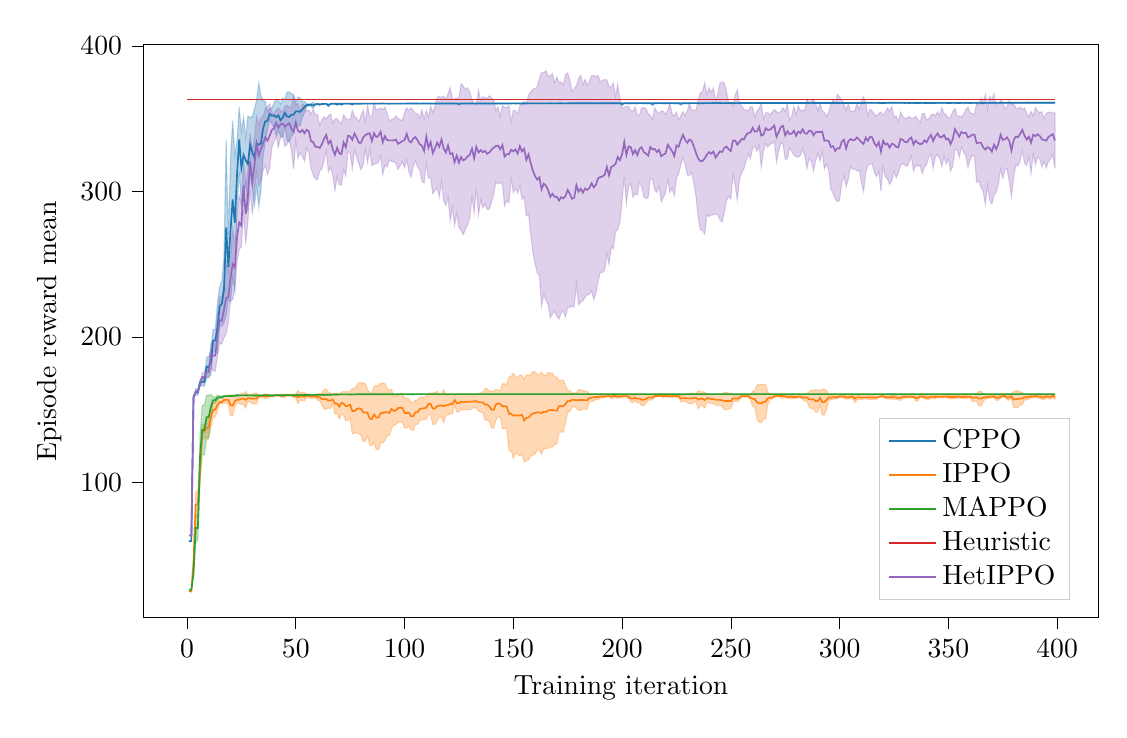
\begin{tikzpicture}

\definecolor{crimson2143940}{RGB}{214,39,40}
\definecolor{darkgray176}{RGB}{176,176,176}
\definecolor{darkorange25512714}{RGB}{255,127,14}
\definecolor{forestgreen4416044}{RGB}{44,160,44}
\definecolor{lightgray204}{RGB}{204,204,204}
\definecolor{mediumpurple148103189}{RGB}{148,103,189}
\definecolor{steelblue31119180}{RGB}{31,119,180}

\begin{axis}[
scale only axis=true,
width=\linewidth,
height=0.6\linewidth,
legend cell align={left},
legend style={
  fill opacity=0.8,
  draw opacity=1,
  text opacity=1,
  at={(0.97,0.03)},
  anchor=south east,
  draw=lightgray204
},
tick align=outside,
tick pos=left,
unbounded coords=jump,
x grid style={darkgray176},
xlabel={Training iteration},
xmin=-19.95, xmax=418.95,
xtick style={color=black},
y grid style={darkgray176},
ylabel={Episode reward mean},
ymin=7.35942219098426, ymax=400.737485807134,
ytick style={color=black}
]
\path [draw=steelblue31119180, fill=steelblue31119180, opacity=0.3]
(axis cs:1,59.409147666913)
--(axis cs:1,60.0415879338764)
--(axis cs:2,60.3519013634999)
--(axis cs:3,159.186012271515)
--(axis cs:4,164.450478074876)
--(axis cs:5,164.268659961843)
--(axis cs:6,170.715512931036)
--(axis cs:7,172.247639830274)
--(axis cs:8,171.82967933804)
--(axis cs:9,186.263868106628)
--(axis cs:10,186.495518283578)
--(axis cs:11,191.35133659168)
--(axis cs:12,205.298455895493)
--(axis cs:13,205.005285611664)
--(axis cs:14,223.4612668043)
--(axis cs:15,234.572675635469)
--(axis cs:16,238.259139951592)
--(axis cs:17,254.892426229319)
--(axis cs:18,335.402206326262)
--(axis cs:19,269.979347200751)
--(axis cs:20,322.101061084545)
--(axis cs:21,348.576030428156)
--(axis cs:22,324.849677309171)
--(axis cs:23,334.642947175794)
--(axis cs:24,357.976343564154)
--(axis cs:25,341.31705013656)
--(axis cs:26,350.737166181143)
--(axis cs:27,336.64108678682)
--(axis cs:28,351.736599064546)
--(axis cs:29,350.922497159108)
--(axis cs:30,351.12963578687)
--(axis cs:31,356.560213117589)
--(axis cs:32,362.732299241753)
--(axis cs:33,374.386756585355)
--(axis cs:34,365.481989967593)
--(axis cs:35,362.143024480451)
--(axis cs:36,361.87227635841)
--(axis cs:37,354.695500515024)
--(axis cs:38,357.239792070042)
--(axis cs:39,357.316927990613)
--(axis cs:40,360.716447250565)
--(axis cs:41,363.541859581334)
--(axis cs:42,362.610520443872)
--(axis cs:43,359.98920832099)
--(axis cs:44,364.083245000427)
--(axis cs:45,363.131646853631)
--(axis cs:46,368.220901401309)
--(axis cs:47,368.3213996845)
--(axis cs:48,367.174950689375)
--(axis cs:49,365.854438647454)
--(axis cs:50,361.223715222184)
--(axis cs:51,364.864701191963)
--(axis cs:52,364.305920945184)
--(axis cs:53,361.744567928832)
--(axis cs:54,361.840691306917)
--(axis cs:55,360.275644597286)
--(axis cs:56,360.072942005302)
--(axis cs:57,360.446644506428)
--(axis cs:58,361.256901960621)
--(axis cs:59,360.234972961485)
--(axis cs:60,360.228360917048)
--(axis cs:61,360.408603022516)
--(axis cs:62,360.081585603453)
--(axis cs:63,360.216468581279)
--(axis cs:64,360.221386589765)
--(axis cs:65,360.081878942931)
--(axis cs:66,360.198627824701)
--(axis cs:67,360.258082126047)
--(axis cs:68,360.345603575512)
--(axis cs:69,360.694407780101)
--(axis cs:70,360.298336835741)
--(axis cs:71,360.666337316544)
--(axis cs:72,360.321837938917)
--(axis cs:73,360.290860426776)
--(axis cs:74,360.312995074438)
--(axis cs:75,360.334977045846)
--(axis cs:76,360.665543738375)
--(axis cs:77,360.348158666494)
--(axis cs:78,360.323495009469)
--(axis cs:79,360.317151061667)
--(axis cs:80,360.351638868156)
--(axis cs:81,360.410620786364)
--(axis cs:82,360.378638189548)
--(axis cs:83,360.330681748349)
--(axis cs:84,360.352196755067)
--(axis cs:85,360.387729337472)
--(axis cs:86,360.354882798699)
--(axis cs:87,360.357989717448)
--(axis cs:88,360.393495315724)
--(axis cs:89,360.397965422908)
--(axis cs:90,360.39244772869)
--(axis cs:91,360.351745705839)
--(axis cs:92,360.382563108489)
--(axis cs:93,360.459296327079)
--(axis cs:94,360.392503394139)
--(axis cs:95,360.366920372264)
--(axis cs:96,360.399280314194)
--(axis cs:97,360.363191194436)
--(axis cs:98,360.404645779941)
--(axis cs:99,360.325638036302)
--(axis cs:100,360.346785243752)
--(axis cs:101,360.390641508306)
--(axis cs:102,360.403494716752)
--(axis cs:103,360.402413790133)
--(axis cs:104,360.443852614657)
--(axis cs:105,360.431597307332)
--(axis cs:106,360.396570775184)
--(axis cs:107,360.382135742526)
--(axis cs:108,360.420833303616)
--(axis cs:109,360.406327985128)
--(axis cs:110,360.430429096667)
--(axis cs:111,360.42526678851)
--(axis cs:112,360.423767539801)
--(axis cs:113,360.390202117045)
--(axis cs:114,360.459744397767)
--(axis cs:115,360.440305431485)
--(axis cs:116,360.435316789234)
--(axis cs:117,360.393669025434)
--(axis cs:118,360.418517440037)
--(axis cs:119,360.454261840124)
--(axis cs:120,360.4413492041)
--(axis cs:121,360.474974757867)
--(axis cs:122,360.406032620258)
--(axis cs:123,360.459118022462)
--(axis cs:124,360.47240813641)
--(axis cs:125,360.706455582743)
--(axis cs:126,360.456476595965)
--(axis cs:127,360.45763973116)
--(axis cs:128,360.508563543231)
--(axis cs:129,360.46937190401)
--(axis cs:130,360.508056060103)
--(axis cs:131,360.54748021621)
--(axis cs:132,360.480565990407)
--(axis cs:133,360.440021787853)
--(axis cs:134,360.554857506486)
--(axis cs:135,360.54498537028)
--(axis cs:136,360.544286705931)
--(axis cs:137,360.547452124484)
--(axis cs:138,360.569642429301)
--(axis cs:139,360.517836444134)
--(axis cs:140,360.513560777358)
--(axis cs:141,360.515108336389)
--(axis cs:142,360.570078922504)
--(axis cs:143,360.553553143293)
--(axis cs:144,360.564238347042)
--(axis cs:145,360.538749959598)
--(axis cs:146,360.542189334302)
--(axis cs:147,360.46800961798)
--(axis cs:148,360.537046229553)
--(axis cs:149,360.557921881664)
--(axis cs:150,360.590424693369)
--(axis cs:151,360.574650237841)
--(axis cs:152,360.633457495684)
--(axis cs:153,360.502826699957)
--(axis cs:154,360.584536665349)
--(axis cs:155,360.481409772727)
--(axis cs:156,360.62752809445)
--(axis cs:157,360.567494421872)
--(axis cs:158,360.587743733294)
--(axis cs:159,360.628207948391)
--(axis cs:160,360.622806665968)
--(axis cs:161,360.550746340413)
--(axis cs:162,360.570981191956)
--(axis cs:163,360.584427641461)
--(axis cs:164,360.581610172349)
--(axis cs:165,360.589960958392)
--(axis cs:166,360.608596199774)
--(axis cs:167,360.652386853138)
--(axis cs:168,360.556648060417)
--(axis cs:169,360.605037159276)
--(axis cs:170,360.637311396029)
--(axis cs:171,360.63394985918)
--(axis cs:172,360.631393274103)
--(axis cs:173,360.660135762513)
--(axis cs:174,360.598317475714)
--(axis cs:175,360.624007930334)
--(axis cs:176,360.731159646062)
--(axis cs:177,360.648865307505)
--(axis cs:178,360.677461838407)
--(axis cs:179,360.686637882291)
--(axis cs:180,360.676143884127)
--(axis cs:181,360.656130424882)
--(axis cs:182,360.714875085432)
--(axis cs:183,360.676754575842)
--(axis cs:184,360.704207683926)
--(axis cs:185,360.696006946257)
--(axis cs:186,360.722940087973)
--(axis cs:187,360.594862143105)
--(axis cs:188,360.664484406225)
--(axis cs:189,360.676280245524)
--(axis cs:190,360.690431882298)
--(axis cs:191,360.708607944687)
--(axis cs:192,360.697970483683)
--(axis cs:193,360.680716262571)
--(axis cs:194,360.768824618487)
--(axis cs:195,360.704570103542)
--(axis cs:196,360.733178680169)
--(axis cs:197,360.702076787736)
--(axis cs:198,360.661159977593)
--(axis cs:199,360.699086488083)
--(axis cs:200,361.184544815968)
--(axis cs:201,360.680121658369)
--(axis cs:202,360.763637312275)
--(axis cs:203,360.720602201487)
--(axis cs:204,360.732949583432)
--(axis cs:205,360.752151992125)
--(axis cs:206,360.711004161072)
--(axis cs:207,360.743473172965)
--(axis cs:208,360.892823162031)
--(axis cs:209,360.755605137347)
--(axis cs:210,360.741662991491)
--(axis cs:211,360.733274125964)
--(axis cs:212,360.718288883598)
--(axis cs:213,360.711821820755)
--(axis cs:214,361.313437679349)
--(axis cs:215,360.753610452497)
--(axis cs:216,360.773578329831)
--(axis cs:217,360.818690900403)
--(axis cs:218,360.742089260121)
--(axis cs:219,360.731547866074)
--(axis cs:220,360.786406267802)
--(axis cs:221,360.73856638806)
--(axis cs:222,360.783491281025)
--(axis cs:223,360.751132517751)
--(axis cs:224,360.745488435513)
--(axis cs:225,360.724584512383)
--(axis cs:226,360.678593413312)
--(axis cs:227,361.11818756822)
--(axis cs:228,360.768875621499)
--(axis cs:229,360.755605323147)
--(axis cs:230,360.725781875061)
--(axis cs:231,360.725222794768)
--(axis cs:232,360.76410024736)
--(axis cs:233,360.753029251521)
--(axis cs:234,360.846246663109)
--(axis cs:235,360.804086121438)
--(axis cs:236,360.757012925136)
--(axis cs:237,360.776319514586)
--(axis cs:238,360.784684098875)
--(axis cs:239,360.786871028039)
--(axis cs:240,360.873574783315)
--(axis cs:241,360.834507178179)
--(axis cs:242,360.890551814682)
--(axis cs:243,360.830430976454)
--(axis cs:244,360.893412046994)
--(axis cs:245,360.888195005251)
--(axis cs:246,360.865405991752)
--(axis cs:247,360.853450652272)
--(axis cs:248,360.874198843887)
--(axis cs:249,360.870925874907)
--(axis cs:250,360.91807859641)
--(axis cs:251,360.904689894267)
--(axis cs:252,360.937745971385)
--(axis cs:253,360.9026608978)
--(axis cs:254,360.935993399542)
--(axis cs:255,360.908396609064)
--(axis cs:256,360.931082757834)
--(axis cs:257,361.004359260366)
--(axis cs:258,360.887732917111)
--(axis cs:259,360.971524442138)
--(axis cs:260,360.867697540568)
--(axis cs:261,360.950389434141)
--(axis cs:262,360.977358078504)
--(axis cs:263,360.934585440999)
--(axis cs:264,360.915735942394)
--(axis cs:265,361.008241764701)
--(axis cs:266,360.99274669614)
--(axis cs:267,360.979381635482)
--(axis cs:268,360.982166425321)
--(axis cs:269,360.935174072344)
--(axis cs:270,360.926546301217)
--(axis cs:271,361.0133075246)
--(axis cs:272,361.007026766209)
--(axis cs:273,360.984614790233)
--(axis cs:274,361.016293730614)
--(axis cs:275,361.011908519098)
--(axis cs:276,360.981408917168)
--(axis cs:277,361.037689378757)
--(axis cs:278,361.01423371129)
--(axis cs:279,360.958158713334)
--(axis cs:280,360.99902158221)
--(axis cs:281,360.962396053757)
--(axis cs:282,360.968701978767)
--(axis cs:283,361.015448609227)
--(axis cs:284,360.988581787585)
--(axis cs:285,360.980822166437)
--(axis cs:286,361.00074883449)
--(axis cs:287,361.03727977002)
--(axis cs:288,361.038258542084)
--(axis cs:289,361.005297319472)
--(axis cs:290,361.044286845115)
--(axis cs:291,361.080874662151)
--(axis cs:292,361.054671275607)
--(axis cs:293,361.067559891753)
--(axis cs:294,361.053497892807)
--(axis cs:295,361.06021426316)
--(axis cs:296,361.001493903173)
--(axis cs:297,361.02203604048)
--(axis cs:298,361.065602056851)
--(axis cs:299,361.015192561456)
--(axis cs:300,361.033679718049)
--(axis cs:301,361.022887023666)
--(axis cs:302,361.069114040727)
--(axis cs:303,361.021604824095)
--(axis cs:304,360.995295574653)
--(axis cs:305,361.046520543331)
--(axis cs:306,361.036299475086)
--(axis cs:307,361.052895737048)
--(axis cs:308,361.073894126683)
--(axis cs:309,361.092866475784)
--(axis cs:310,360.995204706705)
--(axis cs:311,361.028475161465)
--(axis cs:312,361.089976272668)
--(axis cs:313,361.052900408528)
--(axis cs:314,361.029873474984)
--(axis cs:315,361.14360345036)
--(axis cs:316,361.138363741852)
--(axis cs:317,361.17341024367)
--(axis cs:318,361.084217280408)
--(axis cs:319,361.015167891098)
--(axis cs:320,361.021720247614)
--(axis cs:321,361.06064919768)
--(axis cs:322,361.119131318124)
--(axis cs:323,361.188012508729)
--(axis cs:324,361.129806800585)
--(axis cs:325,361.14688456574)
--(axis cs:326,361.164107779968)
--(axis cs:327,361.141935426883)
--(axis cs:328,361.110502209024)
--(axis cs:329,361.09911823418)
--(axis cs:330,361.035793531399)
--(axis cs:331,361.082145779991)
--(axis cs:332,361.041057106429)
--(axis cs:333,361.108052648087)
--(axis cs:334,361.096701051568)
--(axis cs:335,361.063141273637)
--(axis cs:336,361.049944911841)
--(axis cs:337,361.052353761048)
--(axis cs:338,361.148381700251)
--(axis cs:339,361.091292452376)
--(axis cs:340,361.155643596288)
--(axis cs:341,361.056281982636)
--(axis cs:342,361.082366302144)
--(axis cs:343,361.117437245484)
--(axis cs:344,361.07456950095)
--(axis cs:345,361.112989020355)
--(axis cs:346,361.11770730124)
--(axis cs:347,361.082369345162)
--(axis cs:348,361.164368501075)
--(axis cs:349,361.108647405038)
--(axis cs:350,361.056312039448)
--(axis cs:351,361.072259043321)
--(axis cs:352,361.089074482901)
--(axis cs:353,361.065718593951)
--(axis cs:354,361.022818967357)
--(axis cs:355,361.053208869582)
--(axis cs:356,361.088837649117)
--(axis cs:357,361.073195764396)
--(axis cs:358,361.063334548294)
--(axis cs:359,361.074414866849)
--(axis cs:360,361.059667349848)
--(axis cs:361,361.058180237277)
--(axis cs:362,361.094386548643)
--(axis cs:363,361.045997287507)
--(axis cs:364,361.054054612275)
--(axis cs:365,361.119484643622)
--(axis cs:366,361.070545856416)
--(axis cs:367,361.071205162705)
--(axis cs:368,361.063314409271)
--(axis cs:369,361.182206885401)
--(axis cs:370,361.125564649972)
--(axis cs:371,361.105104886205)
--(axis cs:372,361.139602987166)
--(axis cs:373,361.159121321278)
--(axis cs:374,361.097990216865)
--(axis cs:375,361.145084979352)
--(axis cs:376,361.069649399554)
--(axis cs:377,361.165872568034)
--(axis cs:378,361.217059049324)
--(axis cs:379,361.147760599719)
--(axis cs:380,361.097490261277)
--(axis cs:381,361.204811844029)
--(axis cs:382,361.159798144289)
--(axis cs:383,361.176015198716)
--(axis cs:384,361.169879304587)
--(axis cs:385,361.153859055108)
--(axis cs:386,361.277539662971)
--(axis cs:387,361.237256682429)
--(axis cs:388,361.148311347164)
--(axis cs:389,361.173992389632)
--(axis cs:390,361.291132839948)
--(axis cs:391,361.183704292555)
--(axis cs:392,361.203317472635)
--(axis cs:393,361.210372525997)
--(axis cs:394,361.251409849517)
--(axis cs:395,361.225344649341)
--(axis cs:396,361.274475998023)
--(axis cs:397,361.240635861898)
--(axis cs:398,361.178934469032)
--(axis cs:399,361.234376554466)
--(axis cs:399,360.655702024551)
--(axis cs:399,360.655702024551)
--(axis cs:398,360.624326853648)
--(axis cs:397,360.532726119294)
--(axis cs:396,360.605478147367)
--(axis cs:395,360.540528699139)
--(axis cs:394,360.602257389178)
--(axis cs:393,360.567478495499)
--(axis cs:392,360.529255445808)
--(axis cs:391,360.562955900313)
--(axis cs:390,360.594581873935)
--(axis cs:389,360.585363667218)
--(axis cs:388,360.654961365004)
--(axis cs:387,360.538955440826)
--(axis cs:386,360.535312065356)
--(axis cs:385,360.534281406118)
--(axis cs:384,360.504588340858)
--(axis cs:383,360.587818652242)
--(axis cs:382,360.556829901983)
--(axis cs:381,360.547738310361)
--(axis cs:380,360.546643148428)
--(axis cs:379,360.603435058706)
--(axis cs:378,360.547855448387)
--(axis cs:377,360.524513985788)
--(axis cs:376,360.55473380883)
--(axis cs:375,360.475557431798)
--(axis cs:374,360.513871635818)
--(axis cs:373,360.491121606858)
--(axis cs:372,360.535014984273)
--(axis cs:371,360.493860462978)
--(axis cs:370,360.492631957745)
--(axis cs:369,360.470673408112)
--(axis cs:368,360.600530561334)
--(axis cs:367,360.504935439799)
--(axis cs:366,360.43974700096)
--(axis cs:365,360.434788914965)
--(axis cs:364,360.585013607089)
--(axis cs:363,360.503767515575)
--(axis cs:362,360.498617776473)
--(axis cs:361,360.529109725952)
--(axis cs:360,360.44675661428)
--(axis cs:359,360.514983989127)
--(axis cs:358,360.498442634378)
--(axis cs:357,360.530818257927)
--(axis cs:356,360.482112677688)
--(axis cs:355,360.481376817491)
--(axis cs:354,360.535934149534)
--(axis cs:353,360.504786663838)
--(axis cs:352,360.490534706919)
--(axis cs:351,360.482264799762)
--(axis cs:350,360.435264161909)
--(axis cs:349,360.460109626034)
--(axis cs:348,360.500509893098)
--(axis cs:347,360.567656966348)
--(axis cs:346,360.515270146081)
--(axis cs:345,360.477277111873)
--(axis cs:344,360.473480798794)
--(axis cs:343,360.456385796909)
--(axis cs:342,360.430515832617)
--(axis cs:341,360.498526432966)
--(axis cs:340,360.385298466275)
--(axis cs:339,360.451760645126)
--(axis cs:338,360.501650919092)
--(axis cs:337,360.454130002947)
--(axis cs:336,360.490787212809)
--(axis cs:335,360.503404262757)
--(axis cs:334,360.438442549415)
--(axis cs:333,360.55065367874)
--(axis cs:332,360.456441024439)
--(axis cs:331,360.51043858829)
--(axis cs:330,360.50298174321)
--(axis cs:329,360.564971924238)
--(axis cs:328,360.605548465452)
--(axis cs:327,360.535014780112)
--(axis cs:326,360.549470073677)
--(axis cs:325,360.578122804869)
--(axis cs:324,360.576180916413)
--(axis cs:323,360.549691388741)
--(axis cs:322,360.532413037587)
--(axis cs:321,360.472316876753)
--(axis cs:320,360.519927032833)
--(axis cs:319,360.468653611289)
--(axis cs:318,360.485837166177)
--(axis cs:317,360.505616939008)
--(axis cs:316,360.543772147663)
--(axis cs:315,360.538986260227)
--(axis cs:314,360.547673637769)
--(axis cs:313,360.56335641172)
--(axis cs:312,360.515469746111)
--(axis cs:311,360.500260062615)
--(axis cs:310,360.541088544183)
--(axis cs:309,360.472002068828)
--(axis cs:308,360.484468246998)
--(axis cs:307,360.447409270117)
--(axis cs:306,360.477026056281)
--(axis cs:305,360.512556128795)
--(axis cs:304,360.40239419911)
--(axis cs:303,360.542036744795)
--(axis cs:302,360.455821677289)
--(axis cs:301,360.526605217743)
--(axis cs:300,360.462292580581)
--(axis cs:299,360.528660704284)
--(axis cs:298,360.496592759044)
--(axis cs:297,360.454779755947)
--(axis cs:296,360.497646797398)
--(axis cs:295,360.453539179983)
--(axis cs:294,360.496310035547)
--(axis cs:293,360.492242208065)
--(axis cs:292,360.472177442989)
--(axis cs:291,360.458523242306)
--(axis cs:290,360.499896686507)
--(axis cs:289,360.524491639537)
--(axis cs:288,360.441705229302)
--(axis cs:287,360.565340017721)
--(axis cs:286,360.525359796396)
--(axis cs:285,360.495521828142)
--(axis cs:284,360.467883959328)
--(axis cs:283,360.481446543553)
--(axis cs:282,360.518811503269)
--(axis cs:281,360.446198305356)
--(axis cs:280,360.455949787697)
--(axis cs:279,360.442853236348)
--(axis cs:278,360.506753884175)
--(axis cs:277,360.498247381231)
--(axis cs:276,360.5226330058)
--(axis cs:275,360.477288434633)
--(axis cs:274,360.445797094374)
--(axis cs:273,360.501468798236)
--(axis cs:272,360.478667644633)
--(axis cs:271,360.482148073541)
--(axis cs:270,360.522024904279)
--(axis cs:269,360.580865340486)
--(axis cs:268,360.516199033355)
--(axis cs:267,360.489351758922)
--(axis cs:266,360.576009671455)
--(axis cs:265,360.491250404209)
--(axis cs:264,360.625835703171)
--(axis cs:263,360.434608944151)
--(axis cs:262,360.445791101022)
--(axis cs:261,360.467551916782)
--(axis cs:260,360.434937212131)
--(axis cs:259,360.480220575707)
--(axis cs:258,360.43683087015)
--(axis cs:257,360.455606005866)
--(axis cs:256,360.398998470444)
--(axis cs:255,360.502486821838)
--(axis cs:254,360.430551853114)
--(axis cs:253,360.369965286088)
--(axis cs:252,360.398362314445)
--(axis cs:251,360.427978372808)
--(axis cs:250,360.474759407702)
--(axis cs:249,360.459545330055)
--(axis cs:248,360.471078941439)
--(axis cs:247,360.45956964753)
--(axis cs:246,360.435539843796)
--(axis cs:245,360.496964725683)
--(axis cs:244,360.439945759118)
--(axis cs:243,360.461597117416)
--(axis cs:242,360.490841968644)
--(axis cs:241,360.468103823363)
--(axis cs:240,360.423152894287)
--(axis cs:239,360.463136860669)
--(axis cs:238,360.419093075807)
--(axis cs:237,360.446603063999)
--(axis cs:236,360.407297381513)
--(axis cs:235,360.420939582302)
--(axis cs:234,360.441858508484)
--(axis cs:233,360.459691366551)
--(axis cs:232,360.519601856246)
--(axis cs:231,360.449208102965)
--(axis cs:230,360.352045853207)
--(axis cs:229,360.408491698705)
--(axis cs:228,360.40786323617)
--(axis cs:227,359.186199770228)
--(axis cs:226,360.392908320461)
--(axis cs:225,360.404544441771)
--(axis cs:224,360.40951770649)
--(axis cs:223,360.510819065681)
--(axis cs:222,360.43049675122)
--(axis cs:221,360.475582535866)
--(axis cs:220,360.390743086099)
--(axis cs:219,360.404659159177)
--(axis cs:218,360.437565418729)
--(axis cs:217,360.492000961159)
--(axis cs:216,360.411940868483)
--(axis cs:215,360.426130829646)
--(axis cs:214,358.900577560674)
--(axis cs:213,360.441251806894)
--(axis cs:212,360.414289287239)
--(axis cs:211,360.365996454451)
--(axis cs:210,360.439706283499)
--(axis cs:209,360.432538302466)
--(axis cs:208,360.430705716658)
--(axis cs:207,360.399329455367)
--(axis cs:206,360.383489073009)
--(axis cs:205,360.433309956593)
--(axis cs:204,360.426636401277)
--(axis cs:203,360.348079256834)
--(axis cs:202,360.442123840474)
--(axis cs:201,360.468974508482)
--(axis cs:200,358.946777817092)
--(axis cs:199,360.431201726492)
--(axis cs:198,360.392790288766)
--(axis cs:197,360.39203705537)
--(axis cs:196,360.418838461562)
--(axis cs:195,360.393463053757)
--(axis cs:194,360.318237444631)
--(axis cs:193,360.395949854661)
--(axis cs:192,360.444293608838)
--(axis cs:191,360.383645218216)
--(axis cs:190,360.37809019905)
--(axis cs:189,360.382539988454)
--(axis cs:188,360.426747087544)
--(axis cs:187,360.382151692724)
--(axis cs:186,360.400361518265)
--(axis cs:185,360.321165992868)
--(axis cs:184,360.35452310852)
--(axis cs:183,360.369526636866)
--(axis cs:182,360.345616238192)
--(axis cs:181,360.364428338946)
--(axis cs:180,360.421685685438)
--(axis cs:179,360.323887587531)
--(axis cs:178,360.365340373666)
--(axis cs:177,360.337498683482)
--(axis cs:176,360.438728867204)
--(axis cs:175,360.317526502697)
--(axis cs:174,360.382010420964)
--(axis cs:173,360.32044858285)
--(axis cs:172,360.386368171865)
--(axis cs:171,360.367271597499)
--(axis cs:170,360.311054171987)
--(axis cs:169,360.380037221231)
--(axis cs:168,360.362992326823)
--(axis cs:167,360.383865867682)
--(axis cs:166,360.301452703233)
--(axis cs:165,360.298221253843)
--(axis cs:164,360.331605280593)
--(axis cs:163,360.374370822805)
--(axis cs:162,360.29864878151)
--(axis cs:161,360.376977876033)
--(axis cs:160,360.335852623366)
--(axis cs:159,360.360265665505)
--(axis cs:158,360.297424036199)
--(axis cs:157,360.349468245408)
--(axis cs:156,360.283771174931)
--(axis cs:155,360.285036163051)
--(axis cs:154,360.292898623075)
--(axis cs:153,360.3362943311)
--(axis cs:152,360.283840245375)
--(axis cs:151,360.267320327637)
--(axis cs:150,360.371492858913)
--(axis cs:149,360.271499982501)
--(axis cs:148,360.362509813984)
--(axis cs:147,360.33484944549)
--(axis cs:146,360.281121425279)
--(axis cs:145,360.33917256265)
--(axis cs:144,360.263317339905)
--(axis cs:143,360.293274691904)
--(axis cs:142,360.235502802767)
--(axis cs:141,360.300643433962)
--(axis cs:140,360.255958416274)
--(axis cs:139,360.271871024091)
--(axis cs:138,360.271885296982)
--(axis cs:137,360.236695742424)
--(axis cs:136,360.254720232767)
--(axis cs:135,360.245115315857)
--(axis cs:134,360.31149138449)
--(axis cs:133,360.337098452355)
--(axis cs:132,360.328090777172)
--(axis cs:131,360.30820153424)
--(axis cs:130,360.250016268809)
--(axis cs:129,360.2893435362)
--(axis cs:128,360.322698066946)
--(axis cs:127,360.326015098534)
--(axis cs:126,360.276624861241)
--(axis cs:125,359.373133555431)
--(axis cs:124,360.280410546782)
--(axis cs:123,360.226244510951)
--(axis cs:122,360.321393914655)
--(axis cs:121,360.267852887453)
--(axis cs:120,360.224031760614)
--(axis cs:119,360.304140579287)
--(axis cs:118,360.239158584204)
--(axis cs:117,360.30681210996)
--(axis cs:116,360.241123211121)
--(axis cs:115,360.283621652491)
--(axis cs:114,360.280325680543)
--(axis cs:113,360.180104876306)
--(axis cs:112,360.256500597254)
--(axis cs:111,360.290280933338)
--(axis cs:110,360.24956693422)
--(axis cs:109,360.278368883904)
--(axis cs:108,360.288238530333)
--(axis cs:107,360.239059238397)
--(axis cs:106,360.29729436793)
--(axis cs:105,360.233018723905)
--(axis cs:104,360.279774756602)
--(axis cs:103,360.282646477099)
--(axis cs:102,360.289388027206)
--(axis cs:101,360.289443729142)
--(axis cs:100,360.238172180166)
--(axis cs:99,360.271420524852)
--(axis cs:98,360.201584453337)
--(axis cs:97,360.253725017613)
--(axis cs:96,360.243011567684)
--(axis cs:95,360.240750294775)
--(axis cs:94,360.233893587767)
--(axis cs:93,360.042357807581)
--(axis cs:92,360.240863103472)
--(axis cs:91,360.259105874219)
--(axis cs:90,360.282033089834)
--(axis cs:89,360.265326487711)
--(axis cs:88,360.223061812568)
--(axis cs:87,360.244724899068)
--(axis cs:86,360.251698639155)
--(axis cs:85,360.250831050861)
--(axis cs:84,360.244972231831)
--(axis cs:83,360.215572248927)
--(axis cs:82,360.185864839506)
--(axis cs:81,360.169566322068)
--(axis cs:80,360.172000224657)
--(axis cs:79,360.209224240695)
--(axis cs:78,360.186105545042)
--(axis cs:77,360.221571542869)
--(axis cs:76,359.194490370166)
--(axis cs:75,360.141104903283)
--(axis cs:74,360.250176089904)
--(axis cs:73,360.24041945291)
--(axis cs:72,360.23051644274)
--(axis cs:71,359.054142310342)
--(axis cs:70,360.1318214449)
--(axis cs:69,358.994071846168)
--(axis cs:68,360.097146688106)
--(axis cs:67,360.115349824507)
--(axis cs:66,360.049081410324)
--(axis cs:65,357.987633989919)
--(axis cs:64,360.063405559872)
--(axis cs:63,360.018003196571)
--(axis cs:62,359.929558954605)
--(axis cs:61,359.003421448043)
--(axis cs:60,359.872794563846)
--(axis cs:59,359.254561749096)
--(axis cs:58,356.807294365136)
--(axis cs:57,358.592976073693)
--(axis cs:56,358.704883218063)
--(axis cs:55,358.341664158172)
--(axis cs:54,354.086784473114)
--(axis cs:53,350.624274595934)
--(axis cs:52,345.063470433799)
--(axis cs:51,345.052548158369)
--(axis cs:50,348.725777023897)
--(axis cs:49,339.503297028404)
--(axis cs:48,338.149377494537)
--(axis cs:47,334.006859371663)
--(axis cs:46,334.705999331576)
--(axis cs:45,345.012623037285)
--(axis cs:44,337.327929312779)
--(axis cs:43,337.65570804437)
--(axis cs:42,341.819735679027)
--(axis cs:41,338.433216669069)
--(axis cs:40,343.951042299472)
--(axis cs:39,346.621405893757)
--(axis cs:38,349.148568997419)
--(axis cs:37,342.136377043203)
--(axis cs:36,334.330842771737)
--(axis cs:35,324.631191772485)
--(axis cs:34,300.631685639956)
--(axis cs:33,289.611948391194)
--(axis cs:32,303.391153866886)
--(axis cs:31,290.425035782931)
--(axis cs:30,302.535877073576)
--(axis cs:29,313.511251063589)
--(axis cs:28,285.823072899141)
--(axis cs:27,305.960171900353)
--(axis cs:26,299.265317438855)
--(axis cs:25,290.701246664977)
--(axis cs:24,313.49405820499)
--(axis cs:23,288.710393282777)
--(axis cs:22,232.149584556552)
--(axis cs:21,240.375512461918)
--(axis cs:20,223.706693614921)
--(axis cs:19,226.253502645473)
--(axis cs:18,215.030866679841)
--(axis cs:17,209.555844987066)
--(axis cs:16,207.459413039202)
--(axis cs:15,207.664550126417)
--(axis cs:14,188.79886306841)
--(axis cs:13,190.399315283741)
--(axis cs:12,190.111269899945)
--(axis cs:11,173.933453546723)
--(axis cs:10,172.620495306042)
--(axis cs:9,172.584560082133)
--(axis cs:8,166.424726311146)
--(axis cs:7,166.29439219101)
--(axis cs:6,167.344407914393)
--(axis cs:5,159.987659458018)
--(axis cs:4,160.016417084209)
--(axis cs:3,158.808327909836)
--(axis cs:2,59.7147372168224)
--(axis cs:1,59.409147666913)
--cycle;

\path [draw=darkorange25512714, fill=darkorange25512714, opacity=0.3]
(axis cs:1,25.487191174131)
--(axis cs:1,25.6458488367981)
--(axis cs:2,25.3993444240004)
--(axis cs:3,47.201931109418)
--(axis cs:4,93.7048140491107)
--(axis cs:5,94.0578479999783)
--(axis cs:6,114.989487906775)
--(axis cs:7,140.008355838896)
--(axis cs:8,139.92294545927)
--(axis cs:9,144.723997725384)
--(axis cs:10,144.522953614231)
--(axis cs:11,153.09979395642)
--(axis cs:12,155.002622088876)
--(axis cs:13,155.089619912959)
--(axis cs:14,157.689874187344)
--(axis cs:15,156.344272720639)
--(axis cs:16,156.085804034039)
--(axis cs:17,158.991990802012)
--(axis cs:18,158.995802045972)
--(axis cs:19,160.229161910764)
--(axis cs:20,160.012078872294)
--(axis cs:21,160.050339121653)
--(axis cs:22,159.676044612951)
--(axis cs:23,159.382205827091)
--(axis cs:24,159.52282119621)
--(axis cs:25,161.401305991172)
--(axis cs:26,161.333503511776)
--(axis cs:27,162.584916632491)
--(axis cs:28,160.322266374731)
--(axis cs:29,160.310306848695)
--(axis cs:30,160.915995099148)
--(axis cs:31,161.572477222694)
--(axis cs:32,161.502610406259)
--(axis cs:33,160.290534025747)
--(axis cs:34,160.256706479666)
--(axis cs:35,160.416830719813)
--(axis cs:36,160.989944195759)
--(axis cs:37,160.964260483032)
--(axis cs:38,160.645394461988)
--(axis cs:39,160.348938623274)
--(axis cs:40,160.337507611128)
--(axis cs:41,160.100637742636)
--(axis cs:42,160.09871419902)
--(axis cs:43,160.350855435598)
--(axis cs:44,160.834041616963)
--(axis cs:45,160.801277577877)
--(axis cs:46,160.322268204977)
--(axis cs:47,160.653246674434)
--(axis cs:48,160.650625951999)
--(axis cs:49,160.756608596691)
--(axis cs:50,160.745036751662)
--(axis cs:51,163.199857785987)
--(axis cs:52,161.71975977165)
--(axis cs:53,161.985984176097)
--(axis cs:54,161.788469637381)
--(axis cs:55,160.934768794078)
--(axis cs:56,160.905836310926)
--(axis cs:57,160.433995825336)
--(axis cs:58,160.418227089357)
--(axis cs:59,160.507884576769)
--(axis cs:60,160.9314292493)
--(axis cs:61,160.919017421226)
--(axis cs:62,161.393111094021)
--(axis cs:63,164.036541703975)
--(axis cs:64,164.309819563025)
--(axis cs:65,161.715579043935)
--(axis cs:66,161.76369596843)
--(axis cs:67,160.357937688473)
--(axis cs:68,161.386881369922)
--(axis cs:69,161.271849365144)
--(axis cs:70,160.554668409128)
--(axis cs:71,162.29059570431)
--(axis cs:72,162.54439298647)
--(axis cs:73,162.436256191218)
--(axis cs:74,162.471349051948)
--(axis cs:75,162.607488552694)
--(axis cs:76,164.87854596292)
--(axis cs:77,164.542612908219)
--(axis cs:78,166.746120353203)
--(axis cs:79,168.640099369558)
--(axis cs:80,168.708423436302)
--(axis cs:81,168.169076679854)
--(axis cs:82,168.204313524748)
--(axis cs:83,163.740527422189)
--(axis cs:84,162.099368570481)
--(axis cs:85,162.01078689913)
--(axis cs:86,165.900308983681)
--(axis cs:87,166.569502630636)
--(axis cs:88,166.810561948344)
--(axis cs:89,168.397647423719)
--(axis cs:90,168.381375984472)
--(axis cs:91,168.056462354543)
--(axis cs:92,164.47429036645)
--(axis cs:93,163.499521598766)
--(axis cs:94,164.147945048123)
--(axis cs:95,159.200902335016)
--(axis cs:96,159.380656025626)
--(axis cs:97,160.83972064954)
--(axis cs:98,161.125890105076)
--(axis cs:99,161.415569387626)
--(axis cs:100,158.05246704348)
--(axis cs:101,157.999766599044)
--(axis cs:102,157.749162095753)
--(axis cs:103,155.110128589709)
--(axis cs:104,155.324956290363)
--(axis cs:105,156.608185913024)
--(axis cs:106,156.871230099296)
--(axis cs:107,158.517153985972)
--(axis cs:108,158.753144309759)
--(axis cs:109,158.722099655715)
--(axis cs:110,159.593056820206)
--(axis cs:111,161.44306818813)
--(axis cs:112,161.3641652841)
--(axis cs:113,161.766306990398)
--(axis cs:114,161.832354089487)
--(axis cs:115,162.79458445027)
--(axis cs:116,160.988615693989)
--(axis cs:117,160.932924390342)
--(axis cs:118,163.724957216659)
--(axis cs:119,159.821740062703)
--(axis cs:120,159.991010442125)
--(axis cs:121,160.724218258343)
--(axis cs:122,160.586236831561)
--(axis cs:123,160.024603879755)
--(axis cs:124,160.544256476238)
--(axis cs:125,160.652819763835)
--(axis cs:126,160.923498241463)
--(axis cs:127,160.657501604396)
--(axis cs:128,160.583640431898)
--(axis cs:129,161.04945379425)
--(axis cs:130,161.139090018678)
--(axis cs:131,160.313994330211)
--(axis cs:132,160.557874291048)
--(axis cs:133,160.620991461125)
--(axis cs:134,161.172224639245)
--(axis cs:135,161.70513374385)
--(axis cs:136,162.097540409544)
--(axis cs:137,164.579940279786)
--(axis cs:138,164.472401204919)
--(axis cs:139,162.589818047773)
--(axis cs:140,162.984581331209)
--(axis cs:141,162.562169043879)
--(axis cs:142,164.221491072362)
--(axis cs:143,163.604954689038)
--(axis cs:144,163.077699076791)
--(axis cs:145,167.873192698311)
--(axis cs:146,167.97711364526)
--(axis cs:147,167.556987726979)
--(axis cs:148,172.584683455279)
--(axis cs:149,172.853715336811)
--(axis cs:150,175.117322592529)
--(axis cs:151,172.546612732041)
--(axis cs:152,172.494912273365)
--(axis cs:153,173.972167568439)
--(axis cs:154,173.743384115964)
--(axis cs:155,171.080775739521)
--(axis cs:156,174.121589931815)
--(axis cs:157,173.862214108291)
--(axis cs:158,174.212952705206)
--(axis cs:159,176.407315356975)
--(axis cs:160,176.101262102457)
--(axis cs:161,174.263251609945)
--(axis cs:162,174.246891971196)
--(axis cs:163,175.939100265274)
--(axis cs:164,173.825964573913)
--(axis cs:165,173.706461043611)
--(axis cs:166,175.632219246634)
--(axis cs:167,175.349283106038)
--(axis cs:168,175.396888573755)
--(axis cs:169,172.51876868519)
--(axis cs:170,172.674434338456)
--(axis cs:171,170.258104380743)
--(axis cs:172,170.295608710778)
--(axis cs:173,170.46504808271)
--(axis cs:174,166.818064233585)
--(axis cs:175,163.420469030633)
--(axis cs:176,163.447331240962)
--(axis cs:177,161.620524015541)
--(axis cs:178,161.61323483925)
--(axis cs:179,161.777857125326)
--(axis cs:180,163.909678585683)
--(axis cs:181,163.847110540006)
--(axis cs:182,163.066418995576)
--(axis cs:183,162.820905460441)
--(axis cs:184,162.894201350216)
--(axis cs:185,160.827545001123)
--(axis cs:186,160.873250540189)
--(axis cs:187,160.933427393349)
--(axis cs:188,160.619143585232)
--(axis cs:189,160.717898573931)
--(axis cs:190,160.080225517493)
--(axis cs:191,160.018204960291)
--(axis cs:192,160.009809982918)
--(axis cs:193,159.831988785598)
--(axis cs:194,159.798784841341)
--(axis cs:195,160.645179563206)
--(axis cs:196,160.947161489389)
--(axis cs:197,160.897749755667)
--(axis cs:198,160.163253209821)
--(axis cs:199,160.182029994952)
--(axis cs:200,160.159583086599)
--(axis cs:201,159.9877219113)
--(axis cs:202,159.983595176854)
--(axis cs:203,160.332139341929)
--(axis cs:204,160.284420554361)
--(axis cs:205,160.369987375335)
--(axis cs:206,159.860176053175)
--(axis cs:207,160.605699157245)
--(axis cs:208,160.607042092873)
--(axis cs:209,160.925510857892)
--(axis cs:210,160.962863453017)
--(axis cs:211,160.267010795855)
--(axis cs:212,160.274054007081)
--(axis cs:213,160.242503468547)
--(axis cs:214,160.030704533248)
--(axis cs:215,159.989123295774)
--(axis cs:216,159.975064205992)
--(axis cs:217,160.418183241526)
--(axis cs:218,160.407040013334)
--(axis cs:219,160.031125973642)
--(axis cs:220,160.121118618933)
--(axis cs:221,160.143048336237)
--(axis cs:222,160.006217928565)
--(axis cs:223,159.896190709486)
--(axis cs:224,159.893113909808)
--(axis cs:225,160.062149284125)
--(axis cs:226,160.055132960858)
--(axis cs:227,160.094766769127)
--(axis cs:228,160.071572291739)
--(axis cs:229,160.022823181507)
--(axis cs:230,161.258473457497)
--(axis cs:231,161.309991386893)
--(axis cs:232,161.617763793054)
--(axis cs:233,161.259699151844)
--(axis cs:234,161.162780485066)
--(axis cs:235,163.23337721927)
--(axis cs:236,162.367987347375)
--(axis cs:237,162.41447388588)
--(axis cs:238,162.219133026118)
--(axis cs:239,160.835408908716)
--(axis cs:240,160.86456814453)
--(axis cs:241,160.563766310864)
--(axis cs:242,160.678679002913)
--(axis cs:243,160.555652199464)
--(axis cs:244,160.753046042279)
--(axis cs:245,160.649937393007)
--(axis cs:246,160.583201436162)
--(axis cs:247,162.031409055347)
--(axis cs:248,162.1373818781)
--(axis cs:249,161.390046756655)
--(axis cs:250,161.489080417603)
--(axis cs:251,160.363749040494)
--(axis cs:252,159.807296651799)
--(axis cs:253,159.83348615512)
--(axis cs:254,160.261456370208)
--(axis cs:255,160.086434475118)
--(axis cs:256,160.100746167468)
--(axis cs:257,160.075244702102)
--(axis cs:258,160.051811741894)
--(axis cs:259,160.074299182136)
--(axis cs:260,162.755143927779)
--(axis cs:261,162.888785844192)
--(axis cs:262,166.975784803755)
--(axis cs:263,167.529103335286)
--(axis cs:264,167.716242245741)
--(axis cs:265,167.39386782539)
--(axis cs:266,167.338836193689)
--(axis cs:267,162.510872788662)
--(axis cs:268,159.803261830907)
--(axis cs:269,159.759285177112)
--(axis cs:270,159.891772915725)
--(axis cs:271,160.045275544947)
--(axis cs:272,160.073386451243)
--(axis cs:273,160.908729544946)
--(axis cs:274,160.831889964941)
--(axis cs:275,160.114407934382)
--(axis cs:276,159.807937003206)
--(axis cs:277,159.90652633197)
--(axis cs:278,160.280909448442)
--(axis cs:279,159.796414815224)
--(axis cs:280,159.77446353473)
--(axis cs:281,159.76130854063)
--(axis cs:282,159.776490841542)
--(axis cs:283,159.821126793173)
--(axis cs:284,161.147047207654)
--(axis cs:285,161.076773117139)
--(axis cs:286,162.464427995113)
--(axis cs:287,163.527875542134)
--(axis cs:288,163.351587571129)
--(axis cs:289,163.750695342578)
--(axis cs:290,163.680643053436)
--(axis cs:291,163.003726318346)
--(axis cs:292,164.263840349981)
--(axis cs:293,164.179685569481)
--(axis cs:294,163.398337566855)
--(axis cs:295,160.232158612933)
--(axis cs:296,160.193790220424)
--(axis cs:297,159.914400431301)
--(axis cs:298,159.905687145591)
--(axis cs:299,159.532993224271)
--(axis cs:300,160.300052994127)
--(axis cs:301,160.284633052772)
--(axis cs:302,160.631397534705)
--(axis cs:303,159.721555236418)
--(axis cs:304,159.704923552792)
--(axis cs:305,160.081856966258)
--(axis cs:306,160.075303434378)
--(axis cs:307,160.436305025923)
--(axis cs:308,160.047825784538)
--(axis cs:309,160.035580476628)
--(axis cs:310,159.848006365947)
--(axis cs:311,159.650790440568)
--(axis cs:312,159.655765376666)
--(axis cs:313,159.856750498664)
--(axis cs:314,159.931593542725)
--(axis cs:315,159.839239882425)
--(axis cs:316,159.636473831761)
--(axis cs:317,159.646413137738)
--(axis cs:318,159.417049787222)
--(axis cs:319,159.962685748375)
--(axis cs:320,159.982981743154)
--(axis cs:321,159.730044540285)
--(axis cs:322,159.872456375587)
--(axis cs:323,159.653715771867)
--(axis cs:324,160.105716890226)
--(axis cs:325,160.241399571147)
--(axis cs:326,160.049180803519)
--(axis cs:327,159.775718703627)
--(axis cs:328,159.858454992113)
--(axis cs:329,160.132348202473)
--(axis cs:330,160.112231857096)
--(axis cs:331,159.798650415899)
--(axis cs:332,159.830731049272)
--(axis cs:333,159.843187998788)
--(axis cs:334,159.612694330456)
--(axis cs:335,160.299492333728)
--(axis cs:336,160.33645523831)
--(axis cs:337,160.014118015709)
--(axis cs:338,160.020880593435)
--(axis cs:339,160.012582428671)
--(axis cs:340,159.905534102835)
--(axis cs:341,159.945191926011)
--(axis cs:342,159.762072638077)
--(axis cs:343,160.016904902465)
--(axis cs:344,160.100766367393)
--(axis cs:345,159.641193545521)
--(axis cs:346,159.639138259955)
--(axis cs:347,159.701540930044)
--(axis cs:348,159.771233592615)
--(axis cs:349,159.808580149845)
--(axis cs:350,160.107036346659)
--(axis cs:351,159.813765092034)
--(axis cs:352,159.821426381227)
--(axis cs:353,160.120251414197)
--(axis cs:354,160.13841547877)
--(axis cs:355,159.93620988756)
--(axis cs:356,159.778584101027)
--(axis cs:357,159.792550321624)
--(axis cs:358,160.083375567503)
--(axis cs:359,159.688729868434)
--(axis cs:360,159.782105841359)
--(axis cs:361,161.092317306355)
--(axis cs:362,160.99522825089)
--(axis cs:363,161.009651998263)
--(axis cs:364,162.797583705888)
--(axis cs:365,162.654514129749)
--(axis cs:366,161.103047646773)
--(axis cs:367,159.799049316961)
--(axis cs:368,159.77521597272)
--(axis cs:369,159.896268090401)
--(axis cs:370,159.872512789467)
--(axis cs:371,160.105019500838)
--(axis cs:372,160.038913532855)
--(axis cs:373,160.013630127746)
--(axis cs:374,160.082313199754)
--(axis cs:375,160.076809724154)
--(axis cs:376,160.081528933641)
--(axis cs:377,160.161199964367)
--(axis cs:378,160.118049252695)
--(axis cs:379,161.0494493702)
--(axis cs:380,162.674637863664)
--(axis cs:381,162.848402298812)
--(axis cs:382,163.391011794176)
--(axis cs:383,162.185402734281)
--(axis cs:384,162.134866108)
--(axis cs:385,160.46561779391)
--(axis cs:386,160.439064883091)
--(axis cs:387,159.977264869003)
--(axis cs:388,160.079993902994)
--(axis cs:389,160.149098086258)
--(axis cs:390,160.473206561915)
--(axis cs:391,160.511636198811)
--(axis cs:392,160.475496457596)
--(axis cs:393,160.224438950219)
--(axis cs:394,160.30008430174)
--(axis cs:395,160.034608647982)
--(axis cs:396,160.383334105357)
--(axis cs:397,160.426827269924)
--(axis cs:398,160.876739234857)
--(axis cs:399,160.228057848129)
--(axis cs:399,157.512602464767)
--(axis cs:399,157.512602464767)
--(axis cs:398,158.304644914306)
--(axis cs:397,157.366187713015)
--(axis cs:396,157.59497091284)
--(axis cs:395,158.442410201632)
--(axis cs:394,156.889110329092)
--(axis cs:393,157.077059742729)
--(axis cs:392,157.993367342274)
--(axis cs:391,157.941250961582)
--(axis cs:390,158.581124402347)
--(axis cs:389,158.220070924858)
--(axis cs:388,158.388833128559)
--(axis cs:387,157.467465946785)
--(axis cs:386,156.924572360418)
--(axis cs:385,157.005115740635)
--(axis cs:384,153.454717318714)
--(axis cs:383,153.39726680075)
--(axis cs:382,151.598599336342)
--(axis cs:381,151.666302946533)
--(axis cs:380,151.625882894635)
--(axis cs:379,157.653360344357)
--(axis cs:378,156.775556464129)
--(axis cs:377,156.726027648491)
--(axis cs:376,158.891734381321)
--(axis cs:375,158.881978080936)
--(axis cs:374,157.885576569093)
--(axis cs:373,156.612335062486)
--(axis cs:372,156.533189101071)
--(axis cs:371,158.412954540409)
--(axis cs:370,158.042062696865)
--(axis cs:369,158.154490721089)
--(axis cs:368,157.631225507499)
--(axis cs:367,157.569125898127)
--(axis cs:366,155.556656658459)
--(axis cs:365,152.788302135178)
--(axis cs:364,152.681391866115)
--(axis cs:363,156.334758135751)
--(axis cs:362,155.75061833951)
--(axis cs:361,155.639991336584)
--(axis cs:360,158.230668619851)
--(axis cs:359,158.172611653641)
--(axis cs:358,157.726284356389)
--(axis cs:357,157.988185318156)
--(axis cs:356,157.942398852103)
--(axis cs:355,158.07893170387)
--(axis cs:354,157.698322739597)
--(axis cs:353,157.659299698517)
--(axis cs:352,157.835612299982)
--(axis cs:351,157.782648269185)
--(axis cs:350,157.797864536045)
--(axis cs:349,158.448910875186)
--(axis cs:348,158.423456502335)
--(axis cs:347,158.153741334407)
--(axis cs:346,158.480642845563)
--(axis cs:345,158.443086528122)
--(axis cs:344,157.659626937432)
--(axis cs:343,157.811595599347)
--(axis cs:342,158.104751756947)
--(axis cs:341,157.017360151238)
--(axis cs:340,157.127567586934)
--(axis cs:339,157.439316645347)
--(axis cs:338,158.510806620641)
--(axis cs:337,158.556777593737)
--(axis cs:336,156.147147256884)
--(axis cs:335,156.046735863489)
--(axis cs:334,158.120048725414)
--(axis cs:333,158.31824891661)
--(axis cs:332,158.267685919908)
--(axis cs:331,158.276125443814)
--(axis cs:330,157.840452192809)
--(axis cs:329,157.738798114167)
--(axis cs:328,156.594963782492)
--(axis cs:327,156.724585103731)
--(axis cs:326,157.143781372338)
--(axis cs:325,157.117796596143)
--(axis cs:324,157.441045665922)
--(axis cs:323,157.435222985911)
--(axis cs:322,157.471561491263)
--(axis cs:321,157.724925599725)
--(axis cs:320,158.61605750716)
--(axis cs:319,158.551898868382)
--(axis cs:318,158.454165966035)
--(axis cs:317,157.152945416148)
--(axis cs:316,157.269904139411)
--(axis cs:315,157.150395863259)
--(axis cs:314,157.089330276817)
--(axis cs:313,157.223777040391)
--(axis cs:312,157.535467724225)
--(axis cs:311,157.430191939047)
--(axis cs:310,157.109051954495)
--(axis cs:309,157.222951852201)
--(axis cs:308,157.148093247593)
--(axis cs:307,155.083110451989)
--(axis cs:306,157.8285712493)
--(axis cs:305,157.817144180408)
--(axis cs:304,157.48696024843)
--(axis cs:303,157.447525513978)
--(axis cs:302,157.786579931039)
--(axis cs:301,158.291255404675)
--(axis cs:300,158.276642552536)
--(axis cs:299,157.824939754349)
--(axis cs:298,157.405229074359)
--(axis cs:297,157.347979983652)
--(axis cs:296,156.788572775319)
--(axis cs:295,156.840504908461)
--(axis cs:294,150.432947758645)
--(axis cs:293,146.528367723747)
--(axis cs:292,146.397078603537)
--(axis cs:291,153.48313424408)
--(axis cs:290,148.591360292054)
--(axis cs:289,148.369392750405)
--(axis cs:288,151.118055468574)
--(axis cs:287,150.73926666678)
--(axis cs:286,152.064404696298)
--(axis cs:285,156.066368235396)
--(axis cs:284,155.92010356831)
--(axis cs:283,157.017509458615)
--(axis cs:282,158.320932883586)
--(axis cs:281,158.269274868342)
--(axis cs:280,157.898734616859)
--(axis cs:279,157.790528205199)
--(axis cs:278,157.69832955498)
--(axis cs:277,157.843923118046)
--(axis cs:276,158.081965506543)
--(axis cs:275,158.43813290682)
--(axis cs:274,158.16534335464)
--(axis cs:273,158.090665450835)
--(axis cs:272,159.174163775207)
--(axis cs:271,159.20306479228)
--(axis cs:270,158.764879036889)
--(axis cs:269,157.107807588457)
--(axis cs:268,156.99799780473)
--(axis cs:267,153.554985746496)
--(axis cs:266,143.719251673809)
--(axis cs:265,143.634618638783)
--(axis cs:264,141.261156367056)
--(axis cs:263,141.572470775513)
--(axis cs:262,143.596463184479)
--(axis cs:261,152.146231675401)
--(axis cs:260,152.525106706598)
--(axis cs:259,156.738249421726)
--(axis cs:258,158.775266089136)
--(axis cs:257,158.755412975002)
--(axis cs:256,158.811449166966)
--(axis cs:255,158.754413685169)
--(axis cs:254,156.720106740628)
--(axis cs:253,155.506834129247)
--(axis cs:252,155.969327694974)
--(axis cs:251,155.443835358863)
--(axis cs:250,150.798973639757)
--(axis cs:249,150.850110056559)
--(axis cs:248,150.016257124641)
--(axis cs:247,150.267541806482)
--(axis cs:246,152.443583875748)
--(axis cs:245,153.080720034304)
--(axis cs:244,153.026369848295)
--(axis cs:243,153.460743114977)
--(axis cs:242,154.127758828012)
--(axis cs:241,154.38452126309)
--(axis cs:240,155.034612451345)
--(axis cs:239,155.094390948523)
--(axis cs:238,151.211185176395)
--(axis cs:237,152.901470195366)
--(axis cs:236,152.942698014982)
--(axis cs:235,150.840556393285)
--(axis cs:234,155.378727368204)
--(axis cs:233,155.382883909165)
--(axis cs:232,154.09898955625)
--(axis cs:231,154.337685871385)
--(axis cs:230,154.684063413142)
--(axis cs:229,155.948936788681)
--(axis cs:228,155.821571456505)
--(axis cs:227,155.57334715109)
--(axis cs:226,158.688149464545)
--(axis cs:225,158.673098990976)
--(axis cs:224,158.86050234929)
--(axis cs:223,158.86715628543)
--(axis cs:222,158.59414654291)
--(axis cs:221,159.022934055598)
--(axis cs:220,158.992531668258)
--(axis cs:219,158.657655397077)
--(axis cs:218,159.060914385805)
--(axis cs:217,159.056429386429)
--(axis cs:216,159.065950893444)
--(axis cs:215,159.037557803468)
--(axis cs:214,156.940280947646)
--(axis cs:213,156.683352669176)
--(axis cs:212,156.595092084627)
--(axis cs:211,154.746559990909)
--(axis cs:210,152.877572739734)
--(axis cs:209,152.994959075607)
--(axis cs:208,154.825378782855)
--(axis cs:207,154.81305420812)
--(axis cs:206,156.582626192243)
--(axis cs:205,155.092385929032)
--(axis cs:204,155.36330863881)
--(axis cs:203,157.719832577905)
--(axis cs:202,158.904351126037)
--(axis cs:201,158.921830618154)
--(axis cs:200,158.333547876249)
--(axis cs:199,158.29818538812)
--(axis cs:198,158.10087369247)
--(axis cs:197,158.078956741331)
--(axis cs:196,158.038571271435)
--(axis cs:195,157.685813577532)
--(axis cs:194,159.106803353983)
--(axis cs:193,159.094546217289)
--(axis cs:192,158.315660028316)
--(axis cs:191,158.262355031506)
--(axis cs:190,158.065786408741)
--(axis cs:189,157.000565919821)
--(axis cs:188,157.157290215425)
--(axis cs:187,156.314185199726)
--(axis cs:186,155.782570764133)
--(axis cs:185,155.81575666466)
--(axis cs:184,150.393820474144)
--(axis cs:183,150.533115676519)
--(axis cs:182,150.488824350022)
--(axis cs:181,149.715755801764)
--(axis cs:180,149.574166784518)
--(axis cs:179,151.391261338667)
--(axis cs:178,152.179458930682)
--(axis cs:177,152.107785558686)
--(axis cs:176,148.675959309747)
--(axis cs:175,148.597153717136)
--(axis cs:174,141.199383087469)
--(axis cs:173,134.631852489768)
--(axis cs:172,134.95009931242)
--(axis cs:171,134.70758847514)
--(axis cs:170,126.351169460321)
--(axis cs:169,126.419667233306)
--(axis cs:168,124.44663361476)
--(axis cs:167,124.440879228646)
--(axis cs:166,123.601628423623)
--(axis cs:165,123.335856020197)
--(axis cs:164,123.549453753836)
--(axis cs:163,119.57456195129)
--(axis cs:162,122.25972088996)
--(axis cs:161,122.473722438173)
--(axis cs:160,119.619679875043)
--(axis cs:159,118.796575113192)
--(axis cs:158,118.37275361849)
--(axis cs:157,115.701637601075)
--(axis cs:156,114.98025307261)
--(axis cs:155,114.319590948626)
--(axis cs:154,119.321925489634)
--(axis cs:153,118.372468347814)
--(axis cs:152,119.54476384334)
--(axis cs:151,120.171817579688)
--(axis cs:150,116.840631446648)
--(axis cs:149,121.865178266276)
--(axis cs:148,122.100014854471)
--(axis cs:147,137.080796329387)
--(axis cs:146,137.010401134307)
--(axis cs:145,137.018350305109)
--(axis cs:144,145.054588861804)
--(axis cs:143,145.162157794543)
--(axis cs:142,143.108922005906)
--(axis cs:141,137.577355895181)
--(axis cs:140,137.40602119039)
--(axis cs:139,141.938718324113)
--(axis cs:138,142.997907548333)
--(axis cs:137,142.841142617947)
--(axis cs:136,148.095504410288)
--(axis cs:135,148.623776934775)
--(axis cs:134,149.173287773244)
--(axis cs:133,151.424401526603)
--(axis cs:132,151.310905298684)
--(axis cs:131,151.163845181918)
--(axis cs:130,150.018441977095)
--(axis cs:129,150.128870192379)
--(axis cs:128,150.28254838155)
--(axis cs:127,149.933177337063)
--(axis cs:126,150.387765727084)
--(axis cs:125,148.35884713966)
--(axis cs:124,148.65116799357)
--(axis cs:123,153.418294619714)
--(axis cs:122,147.525929912612)
--(axis cs:121,147.334791726724)
--(axis cs:120,146.44260172571)
--(axis cs:119,146.639683028887)
--(axis cs:118,141.224815032007)
--(axis cs:117,145.14212447593)
--(axis cs:116,144.850817432162)
--(axis cs:115,142.321971847717)
--(axis cs:114,140.067294071447)
--(axis cs:113,139.946103576309)
--(axis cs:112,146.85721985155)
--(axis cs:111,146.86377095014)
--(axis cs:110,143.404647256064)
--(axis cs:109,143.558618825826)
--(axis cs:108,143.015087847074)
--(axis cs:107,142.952900064315)
--(axis cs:106,139.977357426787)
--(axis cs:105,140.172798452667)
--(axis cs:104,135.831142193438)
--(axis cs:103,136.189257445942)
--(axis cs:102,138.424963588051)
--(axis cs:101,137.541737424627)
--(axis cs:100,137.744125979984)
--(axis cs:99,141.592152329532)
--(axis cs:98,141.856915767186)
--(axis cs:97,141.565977674859)
--(axis cs:96,139.697848818086)
--(axis cs:95,139.440750564468)
--(axis cs:94,136.984133261731)
--(axis cs:93,132.241959204724)
--(axis cs:92,132.384329037886)
--(axis cs:91,128.776339797097)
--(axis cs:90,127.422277214307)
--(axis cs:89,127.140128374982)
--(axis cs:88,122.542876572237)
--(axis cs:87,122.767733642312)
--(axis cs:86,127.756597019141)
--(axis cs:85,125.509167736967)
--(axis cs:84,125.743260276085)
--(axis cs:83,132.248407945015)
--(axis cs:82,128.405827625011)
--(axis cs:81,128.378812308154)
--(axis cs:80,132.682000615579)
--(axis cs:79,133.380608409695)
--(axis cs:78,134.420966405758)
--(axis cs:77,133.834494076635)
--(axis cs:76,133.612374649048)
--(axis cs:75,144.410548463499)
--(axis cs:74,142.95830525661)
--(axis cs:73,142.555727243588)
--(axis cs:72,146.325267422027)
--(axis cs:71,147.117208350209)
--(axis cs:70,143.835014119745)
--(axis cs:69,147.43660244474)
--(axis cs:68,147.243168345517)
--(axis cs:67,153.97855662834)
--(axis cs:66,151.04322544228)
--(axis cs:65,151.082006679521)
--(axis cs:64,150.629398116922)
--(axis cs:63,150.628289410803)
--(axis cs:62,153.683352019207)
--(axis cs:61,156.488606589814)
--(axis cs:60,156.342176179336)
--(axis cs:59,158.561117534983)
--(axis cs:58,157.928581105757)
--(axis cs:57,157.871584887519)
--(axis cs:56,158.478775221613)
--(axis cs:55,158.405448674406)
--(axis cs:54,156.278590130362)
--(axis cs:53,156.361674492361)
--(axis cs:52,156.958411398294)
--(axis cs:51,154.211220093382)
--(axis cs:50,158.265977669325)
--(axis cs:49,158.204548779877)
--(axis cs:48,159.596760557628)
--(axis cs:47,159.629425044579)
--(axis cs:46,159.766164261479)
--(axis cs:45,158.566266753823)
--(axis cs:44,158.527706691135)
--(axis cs:43,159.011747165851)
--(axis cs:42,159.932031223821)
--(axis cs:41,159.95114131892)
--(axis cs:40,159.173988135768)
--(axis cs:39,159.120107991092)
--(axis cs:38,158.858955853016)
--(axis cs:37,157.860422022098)
--(axis cs:36,157.76803845315)
--(axis cs:35,158.462778378224)
--(axis cs:34,158.642503192546)
--(axis cs:33,158.563822125327)
--(axis cs:32,154.104832825383)
--(axis cs:31,153.888345043211)
--(axis cs:30,154.268073577247)
--(axis cs:29,155.648193407098)
--(axis cs:28,155.618745430822)
--(axis cs:27,151.164103478014)
--(axis cs:26,153.895323058585)
--(axis cs:25,153.678098770067)
--(axis cs:24,154.38184373479)
--(axis cs:23,154.625035148495)
--(axis cs:22,152.20192546337)
--(axis cs:21,145.833598625826)
--(axis cs:20,146.113441888521)
--(axis cs:19,153.808166002804)
--(axis cs:18,154.723172517061)
--(axis cs:17,154.584384708687)
--(axis cs:16,154.320783909396)
--(axis cs:15,154.326989426266)
--(axis cs:14,149.362780163454)
--(axis cs:13,145.230930330895)
--(axis cs:12,144.954376847956)
--(axis cs:11,137.708738974491)
--(axis cs:10,131.360866418842)
--(axis cs:9,130.884666342699)
--(axis cs:8,130.291072148895)
--(axis cs:7,130.032539474129)
--(axis cs:6,100.222427104433)
--(axis cs:5,76.2914864855525)
--(axis cs:4,76.2800464481057)
--(axis cs:3,44.0572209155664)
--(axis cs:2,25.2402432644456)
--(axis cs:1,25.487191174131)
--cycle;

\path [draw=forestgreen4416044, fill=forestgreen4416044, opacity=0.3]
(axis cs:1,25.9150720148452)
--(axis cs:1,26.1339775016737)
--(axis cs:2,26.7303678668679)
--(axis cs:3,37.8654367491981)
--(axis cs:4,78.2344253586916)
--(axis cs:5,77.8867410047602)
--(axis cs:6,132.629480123327)
--(axis cs:7,153.243139240967)
--(axis cs:8,153.352012520897)
--(axis cs:9,160.156367779626)
--(axis cs:10,160.049192510798)
--(axis cs:11,160.715325974524)
--(axis cs:12,158.934820552543)
--(axis cs:13,158.892374070315)
--(axis cs:14,160.153067863287)
--(axis cs:15,159.509369557275)
--(axis cs:16,159.571072410371)
--(axis cs:17,159.713097316135)
--(axis cs:18,159.690930073882)
--(axis cs:19,159.617727537278)
--(axis cs:20,159.85588982006)
--(axis cs:21,159.843754999874)
--(axis cs:22,160.111240557391)
--(axis cs:23,160.357956468958)
--(axis cs:24,160.333147204136)
--(axis cs:25,160.11439765291)
--(axis cs:26,160.085145176082)
--(axis cs:27,160.220923685218)
--(axis cs:28,160.143015811174)
--(axis cs:29,160.174885680282)
--(axis cs:30,160.164197480418)
--(axis cs:31,160.226064833965)
--(axis cs:32,160.21145215882)
--(axis cs:33,160.090916441459)
--(axis cs:34,160.089375372569)
--(axis cs:35,160.247584719526)
--(axis cs:36,160.24234531394)
--(axis cs:37,160.254973119828)
--(axis cs:38,160.310925023693)
--(axis cs:39,160.18944378237)
--(axis cs:40,160.200117025981)
--(axis cs:41,160.428767636451)
--(axis cs:42,160.421252124441)
--(axis cs:43,160.272925856127)
--(axis cs:44,160.354134205334)
--(axis cs:45,160.351517104062)
--(axis cs:46,160.512036900533)
--(axis cs:47,160.390768984163)
--(axis cs:48,160.403784033647)
--(axis cs:49,160.483807125133)
--(axis cs:50,160.490853330163)
--(axis cs:51,160.619069386182)
--(axis cs:52,160.538352015982)
--(axis cs:53,160.535194753183)
--(axis cs:54,160.565139872516)
--(axis cs:55,160.64660783649)
--(axis cs:56,160.641682762145)
--(axis cs:57,160.612071406302)
--(axis cs:58,160.615414503134)
--(axis cs:59,160.701730731737)
--(axis cs:60,160.686875661338)
--(axis cs:61,160.693915338834)
--(axis cs:62,160.637609415361)
--(axis cs:63,160.795046741397)
--(axis cs:64,160.795705084096)
--(axis cs:65,160.670834880462)
--(axis cs:66,160.681969034359)
--(axis cs:67,160.788855853971)
--(axis cs:68,160.697740409128)
--(axis cs:69,160.69846782429)
--(axis cs:70,160.769193846772)
--(axis cs:71,160.726546511762)
--(axis cs:72,160.722592428575)
--(axis cs:73,160.727206626195)
--(axis cs:74,160.727690044408)
--(axis cs:75,160.764148485805)
--(axis cs:76,160.782502445689)
--(axis cs:77,160.786503698675)
--(axis cs:78,160.756126500884)
--(axis cs:79,160.772649974148)
--(axis cs:80,160.773759698127)
--(axis cs:81,160.774471924015)
--(axis cs:82,160.777850189191)
--(axis cs:83,160.794287848763)
--(axis cs:84,160.784927689548)
--(axis cs:85,160.784625228431)
--(axis cs:86,160.785509237694)
--(axis cs:87,160.798324872594)
--(axis cs:88,160.803272080441)
--(axis cs:89,160.789726089945)
--(axis cs:90,160.788766932134)
--(axis cs:91,160.804279606129)
--(axis cs:92,160.7966527446)
--(axis cs:93,160.797431824761)
--(axis cs:94,160.791870101409)
--(axis cs:95,160.801196837083)
--(axis cs:96,160.805031369346)
--(axis cs:97,160.812379152075)
--(axis cs:98,160.81050445296)
--(axis cs:99,160.836392715138)
--(axis cs:100,160.805563284547)
--(axis cs:101,160.808783797388)
--(axis cs:102,160.803422325733)
--(axis cs:103,160.809367655786)
--(axis cs:104,160.812038549801)
--(axis cs:105,160.811146856123)
--(axis cs:106,160.809466879164)
--(axis cs:107,160.811100374276)
--(axis cs:108,160.820278800913)
--(axis cs:109,160.818865406394)
--(axis cs:110,160.816564520069)
--(axis cs:111,160.816463351343)
--(axis cs:112,160.817034238121)
--(axis cs:113,160.817328376533)
--(axis cs:114,160.816879366247)
--(axis cs:115,160.816752921742)
--(axis cs:116,160.822317877722)
--(axis cs:117,160.822382411287)
--(axis cs:118,160.819405111227)
--(axis cs:119,160.819932612583)
--(axis cs:120,160.820429977382)
--(axis cs:121,160.823164634812)
--(axis cs:122,160.823249294517)
--(axis cs:123,160.819865884222)
--(axis cs:124,160.82280816582)
--(axis cs:125,160.823520857816)
--(axis cs:126,160.823822209501)
--(axis cs:127,160.824116476042)
--(axis cs:128,160.824343322653)
--(axis cs:129,160.824328117272)
--(axis cs:130,160.824102267236)
--(axis cs:131,160.830145183611)
--(axis cs:132,160.819442597599)
--(axis cs:133,160.819691576603)
--(axis cs:134,160.822517460549)
--(axis cs:135,160.823077851419)
--(axis cs:136,160.823444214629)
--(axis cs:137,160.82587801466)
--(axis cs:138,160.825599183121)
--(axis cs:139,160.822082714312)
--(axis cs:140,160.823504219363)
--(axis cs:141,160.823450466709)
--(axis cs:142,160.826453432109)
--(axis cs:143,160.822382428618)
--(axis cs:144,160.822932644955)
--(axis cs:145,160.82419457081)
--(axis cs:146,160.824092065238)
--(axis cs:147,160.826740190796)
--(axis cs:148,160.822473479693)
--(axis cs:149,160.822610173307)
--(axis cs:150,160.823138015905)
--(axis cs:151,160.825172907218)
--(axis cs:152,160.825153301836)
--(axis cs:153,160.823347256737)
--(axis cs:154,160.823426459326)
--(axis cs:155,160.823447144854)
--(axis cs:156,160.823961567463)
--(axis cs:157,160.82351613514)
--(axis cs:158,160.825817605416)
--(axis cs:159,160.82420804366)
--(axis cs:160,160.824200717305)
--(axis cs:161,160.824745820468)
--(axis cs:162,160.824529854724)
--(axis cs:163,160.825452098412)
--(axis cs:164,160.82346320472)
--(axis cs:165,160.822955115785)
--(axis cs:166,160.826695577504)
--(axis cs:167,160.823593650915)
--(axis cs:168,160.823697606849)
--(axis cs:169,160.825780439013)
--(axis cs:170,160.825653166604)
--(axis cs:171,160.825968784432)
--(axis cs:172,160.826123679346)
--(axis cs:173,160.825994907812)
--(axis cs:174,160.824907802398)
--(axis cs:175,160.825169110305)
--(axis cs:176,160.825218274445)
--(axis cs:177,160.824061337558)
--(axis cs:178,160.823653547261)
--(axis cs:179,160.824430658184)
--(axis cs:180,160.824800973133)
--(axis cs:181,160.824621836775)
--(axis cs:182,160.824057574539)
--(axis cs:183,160.827627589569)
--(axis cs:184,160.827574833002)
--(axis cs:185,160.825108717662)
--(axis cs:186,160.825510476661)
--(axis cs:187,160.824346359686)
--(axis cs:188,160.824937421571)
--(axis cs:189,160.824912614523)
--(axis cs:190,160.825705515122)
--(axis cs:191,160.825322268174)
--(axis cs:192,160.825238600067)
--(axis cs:193,160.823762804656)
--(axis cs:194,160.823537766746)
--(axis cs:195,160.824461794691)
--(axis cs:196,160.824822693086)
--(axis cs:197,160.824999127424)
--(axis cs:198,160.824792577247)
--(axis cs:199,160.824746676591)
--(axis cs:200,160.82476622164)
--(axis cs:201,160.827016768005)
--(axis cs:202,160.826919966865)
--(axis cs:203,160.825766397044)
--(axis cs:204,160.825011545888)
--(axis cs:205,160.825045255986)
--(axis cs:206,160.826438992275)
--(axis cs:207,160.826593005617)
--(axis cs:208,160.826565590268)
--(axis cs:209,160.828394778845)
--(axis cs:210,160.828295035318)
--(axis cs:211,160.821356768972)
--(axis cs:212,160.82376995176)
--(axis cs:213,160.823659198875)
--(axis cs:214,160.826924710254)
--(axis cs:215,160.826041170682)
--(axis cs:216,160.826024043257)
--(axis cs:217,160.826463368425)
--(axis cs:218,160.826441831137)
--(axis cs:219,160.825500996505)
--(axis cs:220,160.82531447274)
--(axis cs:221,160.825364257309)
--(axis cs:222,160.826011651612)
--(axis cs:223,160.828349675952)
--(axis cs:224,160.828203876244)
--(axis cs:225,160.826914057203)
--(axis cs:226,160.826684475211)
--(axis cs:227,160.826251153606)
--(axis cs:228,160.825907129539)
--(axis cs:229,160.825881322826)
--(axis cs:230,160.825614270015)
--(axis cs:231,160.825943029209)
--(axis cs:232,160.825933213982)
--(axis cs:233,160.826001103146)
--(axis cs:234,160.826088909604)
--(axis cs:235,160.825800895895)
--(axis cs:236,160.822740573417)
--(axis cs:237,160.822827907591)
--(axis cs:238,160.828341595593)
--(axis cs:239,160.82523951059)
--(axis cs:240,160.825295876107)
--(axis cs:241,160.824541500456)
--(axis cs:242,160.824576128881)
--(axis cs:243,160.824857402729)
--(axis cs:244,160.824666003848)
--(axis cs:245,160.824524150577)
--(axis cs:246,160.824736774891)
--(axis cs:247,160.825394042655)
--(axis cs:248,160.825439200234)
--(axis cs:249,160.825941962561)
--(axis cs:250,160.825954964042)
--(axis cs:251,160.825681214013)
--(axis cs:252,160.824077318935)
--(axis cs:253,160.824063296672)
--(axis cs:254,160.824924812696)
--(axis cs:255,160.825365415746)
--(axis cs:256,160.825262834877)
--(axis cs:257,160.82472457152)
--(axis cs:258,160.824711926488)
--(axis cs:259,160.825322779216)
--(axis cs:260,160.826075067894)
--(axis cs:261,160.826018224179)
--(axis cs:262,160.825063561098)
--(axis cs:263,160.82570735251)
--(axis cs:264,160.82573838165)
--(axis cs:265,160.825477983741)
--(axis cs:266,160.825497928912)
--(axis cs:267,160.825609691391)
--(axis cs:268,160.825733925713)
--(axis cs:269,160.82575118283)
--(axis cs:270,160.826328182679)
--(axis cs:271,160.826210954966)
--(axis cs:272,160.826198485817)
--(axis cs:273,160.825830668274)
--(axis cs:274,160.82591818369)
--(axis cs:275,160.826132079982)
--(axis cs:276,160.825925541219)
--(axis cs:277,160.825938369169)
--(axis cs:278,160.825820695774)
--(axis cs:279,160.82586941175)
--(axis cs:280,160.825828138654)
--(axis cs:281,160.824979503735)
--(axis cs:282,160.82496436203)
--(axis cs:283,160.824929115265)
--(axis cs:284,160.825111257162)
--(axis cs:285,160.82515635456)
--(axis cs:286,160.825854371223)
--(axis cs:287,160.82569891872)
--(axis cs:288,160.825618665746)
--(axis cs:289,160.825157263908)
--(axis cs:290,160.825155905691)
--(axis cs:291,160.825758168003)
--(axis cs:292,160.824207246569)
--(axis cs:293,160.824067762022)
--(axis cs:294,160.823786154629)
--(axis cs:295,160.823990680668)
--(axis cs:296,160.824254752714)
--(axis cs:297,160.82274506523)
--(axis cs:298,160.822724614858)
--(axis cs:299,160.825970514479)
--(axis cs:300,160.824438018227)
--(axis cs:301,160.824379318099)
--(axis cs:302,160.825089870165)
--(axis cs:303,160.82326898492)
--(axis cs:304,160.823358338694)
--(axis cs:305,160.823564259434)
--(axis cs:306,160.823794248634)
--(axis cs:307,160.824137153834)
--(axis cs:308,160.829889748493)
--(axis cs:309,160.829687852249)
--(axis cs:310,160.824289212927)
--(axis cs:311,160.822155738048)
--(axis cs:312,160.822249905957)
--(axis cs:313,160.823198980462)
--(axis cs:314,160.823334270899)
--(axis cs:315,160.824439445874)
--(axis cs:316,160.824456923104)
--(axis cs:317,160.824507975679)
--(axis cs:318,160.824318474535)
--(axis cs:319,160.824367940981)
--(axis cs:320,160.824419887904)
--(axis cs:321,160.82190767656)
--(axis cs:322,160.821986083641)
--(axis cs:323,160.823403136281)
--(axis cs:324,160.958126690504)
--(axis cs:325,160.952242926655)
--(axis cs:326,160.822491155675)
--(axis cs:327,160.828070933331)
--(axis cs:328,160.827868546016)
--(axis cs:329,160.823043710523)
--(axis cs:330,160.823087046845)
--(axis cs:331,160.824390552677)
--(axis cs:332,160.824126457925)
--(axis cs:333,160.824187960572)
--(axis cs:334,160.824997098784)
--(axis cs:335,160.82202483023)
--(axis cs:336,160.822341322916)
--(axis cs:337,160.824404526931)
--(axis cs:338,160.824423098475)
--(axis cs:339,160.825257611849)
--(axis cs:340,160.828442986959)
--(axis cs:341,160.828195924042)
--(axis cs:342,160.823928684339)
--(axis cs:343,160.82576873168)
--(axis cs:344,160.825708139673)
--(axis cs:345,160.824981270254)
--(axis cs:346,160.824993420628)
--(axis cs:347,160.827295812177)
--(axis cs:348,160.825123109239)
--(axis cs:349,160.825115007696)
--(axis cs:350,160.825034637194)
--(axis cs:351,160.823678796984)
--(axis cs:352,160.823593759597)
--(axis cs:353,160.825984812278)
--(axis cs:354,160.825928212686)
--(axis cs:355,160.825044059504)
--(axis cs:356,160.824087245391)
--(axis cs:357,160.823458424479)
--(axis cs:358,160.825801765078)
--(axis cs:359,160.827182693798)
--(axis cs:360,160.827642907682)
--(axis cs:361,160.825104680557)
--(axis cs:362,160.825142262796)
--(axis cs:363,160.825768305932)
--(axis cs:364,160.826375994762)
--(axis cs:365,160.826367908296)
--(axis cs:366,160.825562360659)
--(axis cs:367,160.825369902663)
--(axis cs:368,160.82536709752)
--(axis cs:369,160.825693221284)
--(axis cs:370,160.825644830101)
--(axis cs:371,160.826338430271)
--(axis cs:372,160.8247152404)
--(axis cs:373,160.824683028435)
--(axis cs:374,160.825656577763)
--(axis cs:375,160.825807736926)
--(axis cs:376,160.825941495711)
--(axis cs:377,160.826010619074)
--(axis cs:378,160.82606423379)
--(axis cs:379,160.823699291752)
--(axis cs:380,160.824192738942)
--(axis cs:381,160.82386473822)
--(axis cs:382,160.823163232134)
--(axis cs:383,160.826010510796)
--(axis cs:384,160.826022190557)
--(axis cs:385,160.823177138097)
--(axis cs:386,160.823129122945)
--(axis cs:387,160.854548153689)
--(axis cs:388,160.838493840663)
--(axis cs:389,160.840104435614)
--(axis cs:390,160.825715797077)
--(axis cs:391,160.823932690213)
--(axis cs:392,160.823977769307)
--(axis cs:393,160.824540412158)
--(axis cs:394,160.823561728028)
--(axis cs:395,160.838981395762)
--(axis cs:396,160.825773219318)
--(axis cs:397,160.824753612096)
--(axis cs:398,160.85672579877)
--(axis cs:399,160.823720432809)
--(axis cs:399,160.79858256629)
--(axis cs:399,160.79858256629)
--(axis cs:398,160.72583470819)
--(axis cs:397,160.795268308109)
--(axis cs:396,160.79256781434)
--(axis cs:395,160.763287719785)
--(axis cs:394,160.804106063816)
--(axis cs:393,160.804373489588)
--(axis cs:392,160.794685341426)
--(axis cs:391,160.79477534911)
--(axis cs:390,160.791143216758)
--(axis cs:389,160.758678988286)
--(axis cs:388,160.76228171163)
--(axis cs:387,160.728950475742)
--(axis cs:386,160.804356750754)
--(axis cs:385,160.804403524472)
--(axis cs:384,160.805020366206)
--(axis cs:383,160.805027546511)
--(axis cs:382,160.804462948515)
--(axis cs:381,160.804357672459)
--(axis cs:380,160.804301590808)
--(axis cs:379,160.804163072302)
--(axis cs:378,160.80500537156)
--(axis cs:377,160.805009626379)
--(axis cs:376,160.805270490831)
--(axis cs:375,160.805289830652)
--(axis cs:374,160.804393505239)
--(axis cs:373,160.804728659416)
--(axis cs:372,160.804753344655)
--(axis cs:371,160.804898863013)
--(axis cs:370,160.805111462242)
--(axis cs:369,160.804987290112)
--(axis cs:368,160.804672668315)
--(axis cs:367,160.80466253488)
--(axis cs:366,160.804232589627)
--(axis cs:365,160.804981481257)
--(axis cs:364,160.804986180186)
--(axis cs:363,160.805071563448)
--(axis cs:362,160.804209581992)
--(axis cs:361,160.804437625509)
--(axis cs:360,160.80539311212)
--(axis cs:359,160.805766362927)
--(axis cs:358,160.804163505481)
--(axis cs:357,160.804014152616)
--(axis cs:356,160.804305984948)
--(axis cs:355,160.80533132578)
--(axis cs:354,160.801891497092)
--(axis cs:353,160.801679642004)
--(axis cs:352,160.803685359895)
--(axis cs:351,160.803727271162)
--(axis cs:350,160.804515402575)
--(axis cs:349,160.804724286261)
--(axis cs:348,160.804732530993)
--(axis cs:347,160.80431748459)
--(axis cs:346,160.804576665374)
--(axis cs:345,160.804562046607)
--(axis cs:344,160.804875632986)
--(axis cs:343,160.804899290059)
--(axis cs:342,160.804257290715)
--(axis cs:341,160.804101722958)
--(axis cs:340,160.804074109938)
--(axis cs:339,160.80337276302)
--(axis cs:338,160.805444226354)
--(axis cs:337,160.805473686077)
--(axis cs:336,160.804568479044)
--(axis cs:335,160.804579880786)
--(axis cs:334,160.805071503877)
--(axis cs:333,160.804551856571)
--(axis cs:332,160.80459019715)
--(axis cs:331,160.804734319709)
--(axis cs:330,160.804172715442)
--(axis cs:329,160.804151175883)
--(axis cs:328,160.802648149961)
--(axis cs:327,160.802530112655)
--(axis cs:326,160.804361190289)
--(axis cs:325,160.518939333858)
--(axis cs:324,160.506522549672)
--(axis cs:323,160.804726040515)
--(axis cs:322,160.803988771782)
--(axis cs:321,160.803926627037)
--(axis cs:320,160.803973976728)
--(axis cs:319,160.803940131705)
--(axis cs:318,160.805316717919)
--(axis cs:317,160.8048481821)
--(axis cs:316,160.804831886891)
--(axis cs:315,160.80403549995)
--(axis cs:314,160.802671047266)
--(axis cs:313,160.802550945311)
--(axis cs:312,160.804265332328)
--(axis cs:311,160.804192911414)
--(axis cs:310,160.805902413722)
--(axis cs:309,160.800159764901)
--(axis cs:308,160.799957303704)
--(axis cs:307,160.803412206362)
--(axis cs:306,160.804512431091)
--(axis cs:305,160.804441498493)
--(axis cs:304,160.803790918966)
--(axis cs:303,160.803695504699)
--(axis cs:302,160.804468258451)
--(axis cs:301,160.804650010724)
--(axis cs:300,160.804701904332)
--(axis cs:299,160.805406136948)
--(axis cs:298,160.801273612261)
--(axis cs:297,160.801027565858)
--(axis cs:296,160.804890812319)
--(axis cs:295,160.804875691341)
--(axis cs:294,160.804796481886)
--(axis cs:293,160.804163725252)
--(axis cs:292,160.804172741605)
--(axis cs:291,160.804081875681)
--(axis cs:290,160.806252950224)
--(axis cs:289,160.806286892261)
--(axis cs:288,160.80572642512)
--(axis cs:287,160.806072116772)
--(axis cs:286,160.802334576614)
--(axis cs:285,160.802065520631)
--(axis cs:284,160.802883372082)
--(axis cs:283,160.804316051712)
--(axis cs:282,160.803861979599)
--(axis cs:281,160.803726509428)
--(axis cs:280,160.804672714407)
--(axis cs:279,160.804581214465)
--(axis cs:278,160.804483454509)
--(axis cs:277,160.804462436304)
--(axis cs:276,160.804489523374)
--(axis cs:275,160.805461852726)
--(axis cs:274,160.804872803324)
--(axis cs:273,160.804834874904)
--(axis cs:272,160.802444080387)
--(axis cs:271,160.802338275629)
--(axis cs:270,160.80454798593)
--(axis cs:269,160.804271452629)
--(axis cs:268,160.804262940274)
--(axis cs:267,160.804482355764)
--(axis cs:266,160.804299861138)
--(axis cs:265,160.804277354292)
--(axis cs:264,160.802291789744)
--(axis cs:263,160.802717470774)
--(axis cs:262,160.805217008098)
--(axis cs:261,160.800993358673)
--(axis cs:260,160.800888132775)
--(axis cs:259,160.805589681171)
--(axis cs:258,160.805727486105)
--(axis cs:257,160.8059616048)
--(axis cs:256,160.806932571083)
--(axis cs:255,160.807069359686)
--(axis cs:254,160.805139739333)
--(axis cs:253,160.804004120473)
--(axis cs:252,160.80454303987)
--(axis cs:251,160.804103449505)
--(axis cs:250,160.801306111932)
--(axis cs:249,160.801257801492)
--(axis cs:248,160.805860164333)
--(axis cs:247,160.805968504823)
--(axis cs:246,160.801571614117)
--(axis cs:245,160.803438538823)
--(axis cs:244,160.803542827105)
--(axis cs:243,160.804230209304)
--(axis cs:242,160.802494715293)
--(axis cs:241,160.802536088976)
--(axis cs:240,160.801499215522)
--(axis cs:239,160.801621309167)
--(axis cs:238,160.806350723145)
--(axis cs:237,160.80061358592)
--(axis cs:236,160.800942384967)
--(axis cs:235,160.806062415038)
--(axis cs:234,160.801189041636)
--(axis cs:233,160.801827345865)
--(axis cs:232,160.803904842582)
--(axis cs:231,160.803490744249)
--(axis cs:230,160.804152079976)
--(axis cs:229,160.800672737157)
--(axis cs:228,160.800292319563)
--(axis cs:227,160.80681447242)
--(axis cs:226,160.799888071748)
--(axis cs:225,160.799744732611)
--(axis cs:224,160.807704591526)
--(axis cs:223,160.807731105667)
--(axis cs:222,160.803327869518)
--(axis cs:221,160.80355851033)
--(axis cs:220,160.803423207874)
--(axis cs:219,160.806277621195)
--(axis cs:218,160.804569659685)
--(axis cs:217,160.804663027933)
--(axis cs:216,160.805478837793)
--(axis cs:215,160.805490427986)
--(axis cs:214,160.802429697136)
--(axis cs:213,160.802690574532)
--(axis cs:212,160.802421627045)
--(axis cs:211,160.802691486412)
--(axis cs:210,160.804942157313)
--(axis cs:209,160.804390491767)
--(axis cs:208,160.80361819231)
--(axis cs:207,160.803556540152)
--(axis cs:206,160.802864311583)
--(axis cs:205,160.803625469836)
--(axis cs:204,160.803571202386)
--(axis cs:203,160.803394839143)
--(axis cs:202,160.804400714707)
--(axis cs:201,160.804513631119)
--(axis cs:200,160.805360264185)
--(axis cs:199,160.805293020301)
--(axis cs:198,160.803823355913)
--(axis cs:197,160.800642018282)
--(axis cs:196,160.802552216732)
--(axis cs:195,160.804140469137)
--(axis cs:194,160.80482967157)
--(axis cs:193,160.804809021067)
--(axis cs:192,160.803577694603)
--(axis cs:191,160.803510047231)
--(axis cs:190,160.804399044042)
--(axis cs:189,160.805691020788)
--(axis cs:188,160.805569429208)
--(axis cs:187,160.80414281923)
--(axis cs:186,160.80352454083)
--(axis cs:185,160.804113099196)
--(axis cs:184,160.804672963056)
--(axis cs:183,160.804494331016)
--(axis cs:182,160.803278356326)
--(axis cs:181,160.793258066542)
--(axis cs:180,160.792888268833)
--(axis cs:179,160.804214583077)
--(axis cs:178,160.801213663127)
--(axis cs:177,160.801663124613)
--(axis cs:176,160.802354018836)
--(axis cs:175,160.802494298411)
--(axis cs:174,160.804760234699)
--(axis cs:173,160.800794211432)
--(axis cs:172,160.800093546841)
--(axis cs:171,160.803880356411)
--(axis cs:170,160.804521777796)
--(axis cs:169,160.804480296738)
--(axis cs:168,160.806855216694)
--(axis cs:167,160.806639726303)
--(axis cs:166,160.80244526396)
--(axis cs:165,160.800312122355)
--(axis cs:164,160.801266726635)
--(axis cs:163,160.801808608907)
--(axis cs:162,160.805340173772)
--(axis cs:161,160.805219671125)
--(axis cs:160,160.80560888877)
--(axis cs:159,160.80546410864)
--(axis cs:158,160.808337225954)
--(axis cs:157,160.804642131404)
--(axis cs:156,160.804680544554)
--(axis cs:155,160.801589961521)
--(axis cs:154,160.800169710622)
--(axis cs:153,160.800241556111)
--(axis cs:152,160.803210204958)
--(axis cs:151,160.803363821303)
--(axis cs:150,160.803568537097)
--(axis cs:149,160.801670613207)
--(axis cs:148,160.801662208254)
--(axis cs:147,160.797013769138)
--(axis cs:146,160.803497093773)
--(axis cs:145,160.803484583467)
--(axis cs:144,160.803753007778)
--(axis cs:143,160.802888111897)
--(axis cs:142,160.804381221864)
--(axis cs:141,160.803803745194)
--(axis cs:140,160.803564374735)
--(axis cs:139,160.803646091548)
--(axis cs:138,160.801319848022)
--(axis cs:137,160.801066278918)
--(axis cs:136,160.796273838712)
--(axis cs:135,160.796170404668)
--(axis cs:134,160.803119241234)
--(axis cs:133,160.806331832764)
--(axis cs:132,160.806375344523)
--(axis cs:131,160.804826509547)
--(axis cs:130,160.795695260554)
--(axis cs:129,160.797571698625)
--(axis cs:128,160.802756823164)
--(axis cs:127,160.802053833839)
--(axis cs:126,160.798790353772)
--(axis cs:125,160.787685552116)
--(axis cs:124,160.791656718183)
--(axis cs:123,160.795091376366)
--(axis cs:122,160.802025580648)
--(axis cs:121,160.79942281007)
--(axis cs:120,160.790257752931)
--(axis cs:119,160.791564526354)
--(axis cs:118,160.797823660023)
--(axis cs:117,160.793099706843)
--(axis cs:116,160.793317865022)
--(axis cs:115,160.793718833524)
--(axis cs:114,160.792438937815)
--(axis cs:113,160.791972368497)
--(axis cs:112,160.77473179982)
--(axis cs:111,160.774479053821)
--(axis cs:110,160.780284168951)
--(axis cs:109,160.773442604661)
--(axis cs:108,160.773221761099)
--(axis cs:107,160.785446663087)
--(axis cs:106,160.768849466051)
--(axis cs:105,160.768792822188)
--(axis cs:104,160.744454570393)
--(axis cs:103,160.745202880033)
--(axis cs:102,160.751508281745)
--(axis cs:101,160.765865350599)
--(axis cs:100,160.765891483832)
--(axis cs:99,160.763870570002)
--(axis cs:98,160.751683247311)
--(axis cs:97,160.747828098143)
--(axis cs:96,160.739010483605)
--(axis cs:95,160.736281277085)
--(axis cs:94,160.71381956675)
--(axis cs:93,160.726393551273)
--(axis cs:92,160.728282001725)
--(axis cs:91,160.675260093724)
--(axis cs:90,160.674921028968)
--(axis cs:89,160.679843160996)
--(axis cs:88,160.679933216553)
--(axis cs:87,160.685327202538)
--(axis cs:86,160.675076691759)
--(axis cs:85,160.641629539941)
--(axis cs:84,160.639944778367)
--(axis cs:83,160.641075692284)
--(axis cs:82,160.613673925418)
--(axis cs:81,160.613034436794)
--(axis cs:80,160.608040464665)
--(axis cs:79,160.616454099098)
--(axis cs:78,160.586683874111)
--(axis cs:77,160.542332344206)
--(axis cs:76,160.538324919232)
--(axis cs:75,160.39483958518)
--(axis cs:74,160.498868512148)
--(axis cs:73,160.507993051252)
--(axis cs:72,160.56925926124)
--(axis cs:71,160.559688368725)
--(axis cs:70,160.514415896148)
--(axis cs:69,160.349438290765)
--(axis cs:68,160.33395626063)
--(axis cs:67,160.238275845054)
--(axis cs:66,160.137132661656)
--(axis cs:65,160.165084599067)
--(axis cs:64,160.084862142314)
--(axis cs:63,160.070874641705)
--(axis cs:62,159.949765137724)
--(axis cs:61,159.998760084788)
--(axis cs:60,159.974779809391)
--(axis cs:59,159.950733536371)
--(axis cs:58,160.040227391207)
--(axis cs:57,160.045991011999)
--(axis cs:56,159.822752169133)
--(axis cs:55,159.811912064349)
--(axis cs:54,159.946710176582)
--(axis cs:53,159.699091445433)
--(axis cs:52,159.6751141316)
--(axis cs:51,160.06573129827)
--(axis cs:50,159.80127757165)
--(axis cs:49,159.819477753399)
--(axis cs:48,159.662117477069)
--(axis cs:47,159.65604218423)
--(axis cs:46,159.910504159021)
--(axis cs:45,159.781207524387)
--(axis cs:44,159.762487194585)
--(axis cs:43,159.758775462793)
--(axis cs:42,159.720820984709)
--(axis cs:41,159.716944068638)
--(axis cs:40,159.540674218526)
--(axis cs:39,159.52693140467)
--(axis cs:38,159.25550418403)
--(axis cs:37,159.736633256343)
--(axis cs:36,159.762698371496)
--(axis cs:35,159.734409728083)
--(axis cs:34,159.728707103093)
--(axis cs:33,159.733100901963)
--(axis cs:32,159.536256621946)
--(axis cs:31,159.526588573589)
--(axis cs:30,159.708766953908)
--(axis cs:29,159.772485466397)
--(axis cs:28,159.777029601903)
--(axis cs:27,159.829791150307)
--(axis cs:26,159.7696764749)
--(axis cs:25,159.804763711526)
--(axis cs:24,159.613714115406)
--(axis cs:23,159.666898446879)
--(axis cs:22,159.45258455817)
--(axis cs:21,159.316050619843)
--(axis cs:20,159.293253619968)
--(axis cs:19,159.23771402307)
--(axis cs:18,159.168232516622)
--(axis cs:17,159.154361424735)
--(axis cs:16,157.799092539523)
--(axis cs:15,157.832484600272)
--(axis cs:14,156.963784276146)
--(axis cs:13,154.549178530546)
--(axis cs:12,154.482283222302)
--(axis cs:11,143.679718757073)
--(axis cs:10,130.217104605482)
--(axis cs:9,129.739653308338)
--(axis cs:8,119.019127088917)
--(axis cs:7,119.330028189891)
--(axis cs:6,103.160622040624)
--(axis cs:5,59.8859741560866)
--(axis cs:4,59.7193522848499)
--(axis cs:3,37.3315882121145)
--(axis cs:2,26.520131038314)
--(axis cs:1,25.9150720148452)
--cycle;

\path [draw=mediumpurple148103189, fill=mediumpurple148103189, opacity=0.3]
(axis cs:1,63.6139294205483)
--(axis cs:1,63.9652221105122)
--(axis cs:2,63.7682149152818)
--(axis cs:3,158.481655409757)
--(axis cs:4,163.524853447461)
--(axis cs:5,163.559335494166)
--(axis cs:6,168.989718081582)
--(axis cs:7,175.519225312032)
--(axis cs:8,175.618123469884)
--(axis cs:9,180.56493479859)
--(axis cs:10,180.229223568899)
--(axis cs:11,195.966908353127)
--(axis cs:12,197.28472869366)
--(axis cs:13,197.976621075268)
--(axis cs:14,214.918424301102)
--(axis cs:15,227.659452505997)
--(axis cs:16,227.371787508698)
--(axis cs:17,237.882827506494)
--(axis cs:18,251.742785870499)
--(axis cs:19,244.914412392534)
--(axis cs:20,255.83024680778)
--(axis cs:21,274.678210646732)
--(axis cs:22,263.334052662305)
--(axis cs:23,285.465999583051)
--(axis cs:24,297.085685325786)
--(axis cs:25,291.116704688617)
--(axis cs:26,321.259919297405)
--(axis cs:27,304.647070174722)
--(axis cs:28,313.974246557936)
--(axis cs:29,340.14982582466)
--(axis cs:30,328.092555227209)
--(axis cs:31,336.490385158208)
--(axis cs:32,351.520304826407)
--(axis cs:33,345.89180278472)
--(axis cs:34,350.658534506234)
--(axis cs:35,351.338536158972)
--(axis cs:36,356.860957931273)
--(axis cs:37,358.144716069765)
--(axis cs:38,360.289873091546)
--(axis cs:39,354.238093138865)
--(axis cs:40,352.933357101489)
--(axis cs:41,356.005016114357)
--(axis cs:42,357.205621706675)
--(axis cs:43,355.691894776308)
--(axis cs:44,354.536388328403)
--(axis cs:45,358.261975487611)
--(axis cs:46,359.287085923496)
--(axis cs:47,357.768035931578)
--(axis cs:48,357.666971397975)
--(axis cs:49,366.513954530948)
--(axis cs:50,359.361336921125)
--(axis cs:51,360.593195499479)
--(axis cs:52,354.631441854321)
--(axis cs:53,360.235279910534)
--(axis cs:54,359.31809155014)
--(axis cs:55,355.331005592277)
--(axis cs:56,355.918910336461)
--(axis cs:57,353.123941475516)
--(axis cs:58,356.272947131569)
--(axis cs:59,352.774407951139)
--(axis cs:60,352.962298326284)
--(axis cs:61,345.660007816374)
--(axis cs:62,349.096154842223)
--(axis cs:63,351.261751716283)
--(axis cs:64,349.767142300047)
--(axis cs:65,351.961398586603)
--(axis cs:66,353.121990839311)
--(axis cs:67,346.973346989843)
--(axis cs:68,349.760261436124)
--(axis cs:69,350.01635376308)
--(axis cs:70,348.033804909098)
--(axis cs:71,346.616834340278)
--(axis cs:72,352.678431712607)
--(axis cs:73,350.342646924464)
--(axis cs:74,349.270173926009)
--(axis cs:75,349.266612249095)
--(axis cs:76,355.622437644296)
--(axis cs:77,351.616114433223)
--(axis cs:78,350.402064287682)
--(axis cs:79,347.71212451975)
--(axis cs:80,351.896111535426)
--(axis cs:81,355.862081710861)
--(axis cs:82,347.969983375776)
--(axis cs:83,359.381855220961)
--(axis cs:84,351.30632327429)
--(axis cs:85,351.621123561396)
--(axis cs:86,361.113086550028)
--(axis cs:87,355.593463067111)
--(axis cs:88,356.553946926448)
--(axis cs:89,357.24322087622)
--(axis cs:90,356.067524338787)
--(axis cs:91,357.949885941694)
--(axis cs:92,353.701064099636)
--(axis cs:93,348.376523697966)
--(axis cs:94,349.391084228199)
--(axis cs:95,349.719538448772)
--(axis cs:96,351.922911526706)
--(axis cs:97,350.350018161127)
--(axis cs:98,349.209290382434)
--(axis cs:99,348.718702061217)
--(axis cs:100,354.291960719654)
--(axis cs:101,357.3268371199)
--(axis cs:102,355.744972533455)
--(axis cs:103,357.389271051719)
--(axis cs:104,355.832553280911)
--(axis cs:105,353.428185663498)
--(axis cs:106,353.397365626681)
--(axis cs:107,350.199357818069)
--(axis cs:108,356.056921834639)
--(axis cs:109,349.801056970682)
--(axis cs:110,355.658390558043)
--(axis cs:111,350.934769566951)
--(axis cs:112,358.500790675566)
--(axis cs:113,354.258475777062)
--(axis cs:114,358.721482017417)
--(axis cs:115,364.627424157961)
--(axis cs:116,365.15496499019)
--(axis cs:117,364.559427178027)
--(axis cs:118,365.374106220398)
--(axis cs:119,363.088826367077)
--(axis cs:120,367.09440104179)
--(axis cs:121,371.274976707731)
--(axis cs:122,363.606738704028)
--(axis cs:123,363.615165551881)
--(axis cs:124,364.010719940529)
--(axis cs:125,364.262061970514)
--(axis cs:126,373.993739429264)
--(axis cs:127,372.276709789628)
--(axis cs:128,370.15131460513)
--(axis cs:129,371.168724623789)
--(axis cs:130,368.243436751672)
--(axis cs:131,362.753528289066)
--(axis cs:132,360.279604569366)
--(axis cs:133,359.380640571674)
--(axis cs:134,369.636180529424)
--(axis cs:135,362.74108279212)
--(axis cs:136,364.952762892159)
--(axis cs:137,364.505913160076)
--(axis cs:138,363.985254134902)
--(axis cs:139,365.679794066775)
--(axis cs:140,364.417962742865)
--(axis cs:141,362.560670131213)
--(axis cs:142,355.66573431388)
--(axis cs:143,357.907348143034)
--(axis cs:144,351.598602058729)
--(axis cs:145,358.956732234786)
--(axis cs:146,357.762092133251)
--(axis cs:147,357.479989194319)
--(axis cs:148,358.98251419358)
--(axis cs:149,347.879678760942)
--(axis cs:150,355.771222152867)
--(axis cs:151,355.391303727399)
--(axis cs:152,353.014565967894)
--(axis cs:153,358.661999195458)
--(axis cs:154,360.4889417947)
--(axis cs:155,361.838785316775)
--(axis cs:156,360.311137469627)
--(axis cs:157,366.227470783999)
--(axis cs:158,368.399299078432)
--(axis cs:159,370.311845740331)
--(axis cs:160,370.556219955625)
--(axis cs:161,371.918005914263)
--(axis cs:162,377.253880660072)
--(axis cs:163,381.83492053915)
--(axis cs:164,381.453387875658)
--(axis cs:165,382.856664733672)
--(axis cs:166,379.616746872437)
--(axis cs:167,379.22416622602)
--(axis cs:168,380.942781809274)
--(axis cs:169,374.86535777108)
--(axis cs:170,378.504760176202)
--(axis cs:171,375.09350535021)
--(axis cs:172,375.279186023013)
--(axis cs:173,373.055991432127)
--(axis cs:174,380.067008410343)
--(axis cs:175,381.346970331989)
--(axis cs:176,376.333509772107)
--(axis cs:177,368.509915736985)
--(axis cs:178,370.580334656351)
--(axis cs:179,372.344970514688)
--(axis cs:180,377.5807287798)
--(axis cs:181,379.808789689637)
--(axis cs:182,373.21111564947)
--(axis cs:183,376.961923940078)
--(axis cs:184,372.938586406526)
--(axis cs:185,375.427231125352)
--(axis cs:186,379.537538730784)
--(axis cs:187,379.780129337015)
--(axis cs:188,378.808680692835)
--(axis cs:189,379.526393744738)
--(axis cs:190,375.18820548827)
--(axis cs:191,376.342703945773)
--(axis cs:192,376.81198532955)
--(axis cs:193,376.613773134686)
--(axis cs:194,372.025856328353)
--(axis cs:195,371.816270057696)
--(axis cs:196,374.584063690068)
--(axis cs:197,365.294407913749)
--(axis cs:198,373.519380431367)
--(axis cs:199,363.931224503465)
--(axis cs:200,357.139492124605)
--(axis cs:201,357.811177551741)
--(axis cs:202,358.399261862137)
--(axis cs:203,358.437789497846)
--(axis cs:204,355.566958562193)
--(axis cs:205,355.078294804002)
--(axis cs:206,358.17214558807)
--(axis cs:207,352.51424389199)
--(axis cs:208,352.412233530235)
--(axis cs:209,357.607915961328)
--(axis cs:210,357.524625924438)
--(axis cs:211,356.8276883428)
--(axis cs:212,353.332412601024)
--(axis cs:213,352.299593007717)
--(axis cs:214,349.275283226684)
--(axis cs:215,357.295329883188)
--(axis cs:216,354.725883529873)
--(axis cs:217,353.48829502744)
--(axis cs:218,355.323228063443)
--(axis cs:219,354.919072018162)
--(axis cs:220,352.898724698897)
--(axis cs:221,355.805955843596)
--(axis cs:222,360.719609412894)
--(axis cs:223,353.18233716025)
--(axis cs:224,351.702545851597)
--(axis cs:225,354.276315434928)
--(axis cs:226,349.142982220664)
--(axis cs:227,351.949738183942)
--(axis cs:228,354.787640483606)
--(axis cs:229,352.09667712052)
--(axis cs:230,355.478018168679)
--(axis cs:231,360.344904286118)
--(axis cs:232,356.11328115968)
--(axis cs:233,355.714856565856)
--(axis cs:234,356.060116709192)
--(axis cs:235,363.17673982754)
--(axis cs:236,367.83982533012)
--(axis cs:237,368.485234694187)
--(axis cs:238,374.66857311494)
--(axis cs:239,366.533786790161)
--(axis cs:240,371.254806903111)
--(axis cs:241,368.115406471931)
--(axis cs:242,370.983197456241)
--(axis cs:243,361.794877333448)
--(axis cs:244,367.106242117442)
--(axis cs:245,374.388844346697)
--(axis cs:246,375.20731563231)
--(axis cs:247,374.471072435341)
--(axis cs:248,368.307194135274)
--(axis cs:249,361.080767224818)
--(axis cs:250,360.800830433107)
--(axis cs:251,358.511081072573)
--(axis cs:252,365.945369594951)
--(axis cs:253,369.856167775903)
--(axis cs:254,359.505784952311)
--(axis cs:255,359.241340528012)
--(axis cs:256,355.897355258475)
--(axis cs:257,356.102973388143)
--(axis cs:258,355.018369089794)
--(axis cs:259,358.155929089755)
--(axis cs:260,357.902072334691)
--(axis cs:261,350.927010933735)
--(axis cs:262,355.177681112603)
--(axis cs:263,356.967600137711)
--(axis cs:264,360.362632689789)
--(axis cs:265,350.093146365865)
--(axis cs:266,353.87846099266)
--(axis cs:267,354.085951659502)
--(axis cs:268,352.576284202864)
--(axis cs:269,354.472513801609)
--(axis cs:270,356.19548052195)
--(axis cs:271,354.866436741353)
--(axis cs:272,353.701012651767)
--(axis cs:273,355.075082218375)
--(axis cs:274,357.391133934958)
--(axis cs:275,354.939497273667)
--(axis cs:276,360.253474587142)
--(axis cs:277,348.984372544855)
--(axis cs:278,351.939585121387)
--(axis cs:279,358.408254117848)
--(axis cs:280,352.560010796377)
--(axis cs:281,358.76295232903)
--(axis cs:282,355.217208797369)
--(axis cs:283,356.067909833591)
--(axis cs:284,355.403795747551)
--(axis cs:285,363.622405882582)
--(axis cs:286,360.812696371782)
--(axis cs:287,362.279272800058)
--(axis cs:288,363.271886317496)
--(axis cs:289,360.287286337541)
--(axis cs:290,355.32620437271)
--(axis cs:291,360.676330782895)
--(axis cs:292,355.267976937546)
--(axis cs:293,354.243906199036)
--(axis cs:294,351.208384359914)
--(axis cs:295,354.646955905797)
--(axis cs:296,359.725576975957)
--(axis cs:297,363.257679679471)
--(axis cs:298,360.470167863635)
--(axis cs:299,366.548624208771)
--(axis cs:300,364.866522243416)
--(axis cs:301,362.360363723174)
--(axis cs:302,360.110489374747)
--(axis cs:303,355.729918338078)
--(axis cs:304,360.296848545395)
--(axis cs:305,354.896797118801)
--(axis cs:306,355.107879460744)
--(axis cs:307,355.537053401075)
--(axis cs:308,360.16576930705)
--(axis cs:309,356.373299034945)
--(axis cs:310,361.461545503597)
--(axis cs:311,365.06323019929)
--(axis cs:312,360.929738432173)
--(axis cs:313,351.932568310065)
--(axis cs:314,356.621180887911)
--(axis cs:315,355.085047695572)
--(axis cs:316,353.191102969462)
--(axis cs:317,351.695123342586)
--(axis cs:318,353.570022231845)
--(axis cs:319,354.579026328961)
--(axis cs:320,352.456887054512)
--(axis cs:321,354.469011565818)
--(axis cs:322,357.265313727263)
--(axis cs:323,355.061541713291)
--(axis cs:324,358.270227604075)
--(axis cs:325,350.896031606894)
--(axis cs:326,351.902589849237)
--(axis cs:327,347.819186969453)
--(axis cs:328,354.437435764405)
--(axis cs:329,351.884964424936)
--(axis cs:330,350.068323545273)
--(axis cs:331,350.297559362577)
--(axis cs:332,351.699576921741)
--(axis cs:333,350.011066267961)
--(axis cs:334,350.391159702306)
--(axis cs:335,351.698816147127)
--(axis cs:336,349.217210592564)
--(axis cs:337,347.199273183921)
--(axis cs:338,353.395420885289)
--(axis cs:339,353.633417726595)
--(axis cs:340,349.043493438375)
--(axis cs:341,349.805928978366)
--(axis cs:342,352.536866977929)
--(axis cs:343,353.202312133494)
--(axis cs:344,351.897632847659)
--(axis cs:345,354.494070131417)
--(axis cs:346,352.184772834263)
--(axis cs:347,357.563597887005)
--(axis cs:348,353.616852179375)
--(axis cs:349,352.593054733116)
--(axis cs:350,350.418964385582)
--(axis cs:351,351.028213789651)
--(axis cs:352,354.715798964538)
--(axis cs:353,357.06226793168)
--(axis cs:354,351.996326105703)
--(axis cs:355,351.771852100063)
--(axis cs:356,351.293698122154)
--(axis cs:357,352.904760769978)
--(axis cs:358,356.217418226993)
--(axis cs:359,357.911547576364)
--(axis cs:360,354.299729099809)
--(axis cs:361,353.161143587798)
--(axis cs:362,353.433744237074)
--(axis cs:363,360.042417442087)
--(axis cs:364,359.766583600389)
--(axis cs:365,364.244003632503)
--(axis cs:366,360.369094369658)
--(axis cs:367,366.649986307651)
--(axis cs:368,356.503362438961)
--(axis cs:369,365.320770934102)
--(axis cs:370,363.235604100366)
--(axis cs:371,367.071031513362)
--(axis cs:372,358.37248672535)
--(axis cs:373,360.442071291654)
--(axis cs:374,362.428169201337)
--(axis cs:375,361.63775021428)
--(axis cs:376,356.618732913116)
--(axis cs:377,358.644793745409)
--(axis cs:378,362.162894796276)
--(axis cs:379,359.807021057376)
--(axis cs:380,360.586765095951)
--(axis cs:381,357.090430418063)
--(axis cs:382,356.928892944441)
--(axis cs:383,357.946842601733)
--(axis cs:384,356.261998458285)
--(axis cs:385,357.479601369545)
--(axis cs:386,353.471784952728)
--(axis cs:387,351.249308109274)
--(axis cs:388,355.023898623784)
--(axis cs:389,351.9282495268)
--(axis cs:390,357.686539808999)
--(axis cs:391,355.098609314933)
--(axis cs:392,354.096313124834)
--(axis cs:393,354.752236964714)
--(axis cs:394,350.228636988183)
--(axis cs:395,353.585202387136)
--(axis cs:396,354.455331247264)
--(axis cs:397,354.428756688911)
--(axis cs:398,353.666201942756)
--(axis cs:399,354.1608430003)
--(axis cs:399,315.671220786813)
--(axis cs:399,315.671220786813)
--(axis cs:398,325.047281753235)
--(axis cs:397,322.420738145297)
--(axis cs:396,320.427849425582)
--(axis cs:395,316.101474777735)
--(axis cs:394,320.501561037408)
--(axis cs:393,316.740093990184)
--(axis cs:392,322.092057585702)
--(axis cs:391,323.456913165804)
--(axis cs:390,318.358318448038)
--(axis cs:389,325.930594650118)
--(axis cs:388,312.053592344813)
--(axis cs:387,323.908818485638)
--(axis cs:386,317.791607770576)
--(axis cs:385,319.283615998159)
--(axis cs:384,328.197967686901)
--(axis cs:383,321.107233283472)
--(axis cs:382,317.52757016602)
--(axis cs:381,318.343297750373)
--(axis cs:380,309.678954704566)
--(axis cs:379,296.418550421771)
--(axis cs:378,306.94758966689)
--(axis cs:377,315.565281194088)
--(axis cs:376,315.191230802009)
--(axis cs:375,309.059072549627)
--(axis cs:374,315.430381718592)
--(axis cs:373,304.994337074334)
--(axis cs:372,299.721979295699)
--(axis cs:371,297.302944705439)
--(axis cs:370,291.41539966557)
--(axis cs:369,294.10317282613)
--(axis cs:368,304.26892193327)
--(axis cs:367,290.885135023881)
--(axis cs:366,300.038644496619)
--(axis cs:365,302.59770312954)
--(axis cs:364,307.343436608528)
--(axis cs:363,306.172448135779)
--(axis cs:362,324.384581075945)
--(axis cs:361,324.893406782279)
--(axis cs:360,321.520154992158)
--(axis cs:359,316.344285549507)
--(axis cs:358,324.484632295912)
--(axis cs:357,326.966866369009)
--(axis cs:356,330.344164975104)
--(axis cs:355,323.500420776958)
--(axis cs:354,328.728855020311)
--(axis cs:353,328.421426352615)
--(axis cs:352,317.347816195963)
--(axis cs:351,313.931510626502)
--(axis cs:350,322.172908521784)
--(axis cs:349,318.973415573951)
--(axis cs:348,323.776359072792)
--(axis cs:347,317.146843834161)
--(axis cs:346,322.663955006181)
--(axis cs:345,325.180236781495)
--(axis cs:344,323.712832812142)
--(axis cs:343,315.948403433686)
--(axis cs:342,325.222032900187)
--(axis cs:341,323.88496098795)
--(axis cs:340,318.416037777456)
--(axis cs:339,316.580378795313)
--(axis cs:338,312.18683879221)
--(axis cs:337,317.740530314901)
--(axis cs:336,317.396597006446)
--(axis cs:335,318.006994042674)
--(axis cs:334,314.043903425051)
--(axis cs:333,324.063738635771)
--(axis cs:332,320.296328235161)
--(axis cs:331,317.177577224546)
--(axis cs:330,317.995337984534)
--(axis cs:329,319.274903190868)
--(axis cs:328,317.654992895817)
--(axis cs:327,312.664329243204)
--(axis cs:326,309.326831376471)
--(axis cs:325,313.706419307151)
--(axis cs:324,307.160398653456)
--(axis cs:323,304.960537138808)
--(axis cs:322,308.48350946947)
--(axis cs:321,309.922339906411)
--(axis cs:320,317.215777413786)
--(axis cs:319,300.055800412263)
--(axis cs:318,314.046144927298)
--(axis cs:317,310.301606220764)
--(axis cs:316,312.741123148556)
--(axis cs:315,319.150091629394)
--(axis cs:314,318.547165768796)
--(axis cs:313,317.725401422477)
--(axis cs:312,312.937369187677)
--(axis cs:311,300.19708843621)
--(axis cs:310,306.247756997598)
--(axis cs:309,314.708755961989)
--(axis cs:308,313.996127210387)
--(axis cs:307,315.356109637579)
--(axis cs:306,315.167391112139)
--(axis cs:305,317.084505447709)
--(axis cs:304,308.517821108688)
--(axis cs:303,303.209655473232)
--(axis cs:302,310.766668482175)
--(axis cs:301,305.928419427328)
--(axis cs:300,294.002939641599)
--(axis cs:299,292.968684951973)
--(axis cs:298,295.107676346887)
--(axis cs:297,298.846618353878)
--(axis cs:296,301.377282860055)
--(axis cs:295,314.567753847991)
--(axis cs:294,318.801448078106)
--(axis cs:293,315.447040646263)
--(axis cs:292,327.016553549598)
--(axis cs:291,320.88678169945)
--(axis cs:290,326.227511328393)
--(axis cs:289,321.197938403052)
--(axis cs:288,313.939429743485)
--(axis cs:287,320.646326799555)
--(axis cs:286,322.637437121902)
--(axis cs:285,315.58472319192)
--(axis cs:284,324.311524923426)
--(axis cs:283,329.491677753773)
--(axis cs:282,324.770451842759)
--(axis cs:281,323.624107603543)
--(axis cs:280,323.85719661884)
--(axis cs:279,324.87985476508)
--(axis cs:278,327.616646210293)
--(axis cs:277,329.592315135849)
--(axis cs:276,322.437494982962)
--(axis cs:275,322.013261094035)
--(axis cs:274,332.582446757508)
--(axis cs:273,333.55762740774)
--(axis cs:272,327.712113640959)
--(axis cs:271,320.252314123179)
--(axis cs:270,334.185657169706)
--(axis cs:269,333.099582558538)
--(axis cs:268,332.301329805044)
--(axis cs:267,330.289124730454)
--(axis cs:266,332.924336643795)
--(axis cs:265,327.806494959075)
--(axis cs:264,316.291861445286)
--(axis cs:263,331.937140643789)
--(axis cs:262,327.355157220012)
--(axis cs:261,331.197342594493)
--(axis cs:260,329.49376762262)
--(axis cs:259,322.517191046363)
--(axis cs:258,325.746455304622)
--(axis cs:257,321.084026495307)
--(axis cs:256,315.399114270551)
--(axis cs:255,312.860640224502)
--(axis cs:254,308.629847095354)
--(axis cs:253,294.2210007052)
--(axis cs:252,304.035236583542)
--(axis cs:251,311.262848224547)
--(axis cs:250,294.756844006985)
--(axis cs:249,296.669173226562)
--(axis cs:248,293.343233359179)
--(axis cs:247,285.472738813847)
--(axis cs:246,279.00522161687)
--(axis cs:245,280.554249403743)
--(axis cs:244,283.715917450257)
--(axis cs:243,284.683280729775)
--(axis cs:242,283.808979287806)
--(axis cs:241,283.703797371685)
--(axis cs:240,282.799691973617)
--(axis cs:239,284.012840809382)
--(axis cs:238,270.773467742442)
--(axis cs:237,273.370350452988)
--(axis cs:236,273.599007499472)
--(axis cs:235,281.973051857809)
--(axis cs:234,296.5555816764)
--(axis cs:233,305.783173206657)
--(axis cs:232,313.317749046202)
--(axis cs:231,310.903167069566)
--(axis cs:230,311.366614459072)
--(axis cs:229,318.884580515752)
--(axis cs:228,322.938539178487)
--(axis cs:227,318.488226976953)
--(axis cs:226,312.102336064469)
--(axis cs:225,308.925090174593)
--(axis cs:224,296.988772138865)
--(axis cs:223,302.291136150444)
--(axis cs:222,299.016969476785)
--(axis cs:221,308.331372545594)
--(axis cs:220,299.26825369749)
--(axis cs:219,295.777588945361)
--(axis cs:218,292.92911574493)
--(axis cs:217,303.657744505244)
--(axis cs:216,299.312337538374)
--(axis cs:215,301.0773164903)
--(axis cs:214,308.38125559857)
--(axis cs:213,308.737457300725)
--(axis cs:212,295.837655933817)
--(axis cs:211,295.081410901049)
--(axis cs:210,296.349780661808)
--(axis cs:209,303.196675637908)
--(axis cs:208,306.182292593609)
--(axis cs:207,297.48667349617)
--(axis cs:206,298.651178105584)
--(axis cs:205,295.994791556293)
--(axis cs:204,305.39565827608)
--(axis cs:203,303.339962132047)
--(axis cs:202,291.715992346676)
--(axis cs:201,309.925395183445)
--(axis cs:200,293.677523078313)
--(axis cs:199,279.014432387102)
--(axis cs:198,273.775608358547)
--(axis cs:197,272.391737644183)
--(axis cs:196,260.59277071724)
--(axis cs:195,261.540428235008)
--(axis cs:194,249.887405552249)
--(axis cs:193,256.985838850735)
--(axis cs:192,245.957134530872)
--(axis cs:191,244.345707081669)
--(axis cs:190,244.461348011064)
--(axis cs:189,238.692890605819)
--(axis cs:188,230.451126014258)
--(axis cs:187,225.772391367759)
--(axis cs:186,231.668587135544)
--(axis cs:185,229.378984350754)
--(axis cs:184,229.17034022953)
--(axis cs:183,227.126730149639)
--(axis cs:182,225.102104042325)
--(axis cs:181,223.855051275623)
--(axis cs:180,222.190070927657)
--(axis cs:179,236.178793962908)
--(axis cs:178,220.723795287481)
--(axis cs:177,221.29675249444)
--(axis cs:176,220.244357958413)
--(axis cs:175,220.528107295026)
--(axis cs:174,213.707269790895)
--(axis cs:173,217.564231589786)
--(axis cs:172,216.724163154247)
--(axis cs:171,212.339245695167)
--(axis cs:170,214.217442891224)
--(axis cs:169,217.773383238856)
--(axis cs:168,215.794431962214)
--(axis cs:167,213.296655909924)
--(axis cs:166,222.442188565331)
--(axis cs:165,225.079705642781)
--(axis cs:164,229.309853390575)
--(axis cs:163,221.169160449417)
--(axis cs:162,242.247684862049)
--(axis cs:161,244.173552901359)
--(axis cs:160,250.655686331437)
--(axis cs:159,258.110260714003)
--(axis cs:158,270.584173491885)
--(axis cs:157,284.607561565096)
--(axis cs:156,283.124272565223)
--(axis cs:155,296.626415814924)
--(axis cs:154,294.473218430196)
--(axis cs:153,303.564667085458)
--(axis cs:152,298.978802506028)
--(axis cs:151,302.210110189965)
--(axis cs:150,299.231697885278)
--(axis cs:149,309.364696261528)
--(axis cs:148,292.294634510117)
--(axis cs:147,293.657074872336)
--(axis cs:146,290.025448612331)
--(axis cs:145,304.845683431264)
--(axis cs:144,306.215572761451)
--(axis cs:143,305.114983601175)
--(axis cs:142,306.662513984936)
--(axis cs:141,297.728464010188)
--(axis cs:140,292.793446155593)
--(axis cs:139,287.897681797164)
--(axis cs:138,287.632592700222)
--(axis cs:137,291.074580083238)
--(axis cs:136,288.920441506229)
--(axis cs:135,294.026589392237)
--(axis cs:134,283.901121839039)
--(axis cs:133,301.810318860786)
--(axis cs:132,285.319211742296)
--(axis cs:131,296.137824567341)
--(axis cs:130,281.986615843888)
--(axis cs:129,276.921556727404)
--(axis cs:128,274.180817062284)
--(axis cs:127,270.397957469795)
--(axis cs:126,273.3340096242)
--(axis cs:125,275.283119875705)
--(axis cs:124,285.173487653681)
--(axis cs:123,276.601933391595)
--(axis cs:122,288.97222777713)
--(axis cs:121,279.949332723525)
--(axis cs:120,296.172511738601)
--(axis cs:119,290.33443227278)
--(axis cs:118,293.394194995513)
--(axis cs:117,306.785497841299)
--(axis cs:116,296.207998294274)
--(axis cs:115,302.456806559387)
--(axis cs:114,300.558547826041)
--(axis cs:113,298.289340555253)
--(axis cs:112,309.347923420919)
--(axis cs:111,309.138081298016)
--(axis cs:110,319.611674742952)
--(axis cs:109,305.749651201614)
--(axis cs:108,306.810703859664)
--(axis cs:107,314.667203690705)
--(axis cs:106,316.727248648194)
--(axis cs:105,321.328009699988)
--(axis cs:104,316.58283887983)
--(axis cs:103,309.857536777507)
--(axis cs:102,313.809086559594)
--(axis cs:101,321.716263817989)
--(axis cs:100,316.183389708054)
--(axis cs:99,320.450895705078)
--(axis cs:98,317.731507498104)
--(axis cs:97,315.038557407478)
--(axis cs:96,319.463117361468)
--(axis cs:95,320.304544502663)
--(axis cs:94,320.672690625065)
--(axis cs:93,321.796811767035)
--(axis cs:92,316.722328467599)
--(axis cs:91,317.990970015032)
--(axis cs:90,311.512525028475)
--(axis cs:89,324.650095513534)
--(axis cs:88,319.883648659396)
--(axis cs:87,319.087981266432)
--(axis cs:86,318.808275867289)
--(axis cs:85,317.642531724831)
--(axis cs:84,328.613457345812)
--(axis cs:83,319.743537482343)
--(axis cs:82,329.349732797324)
--(axis cs:81,318.392900067471)
--(axis cs:80,314.988827595208)
--(axis cs:79,319.012782536965)
--(axis cs:78,323.366563370696)
--(axis cs:77,328.044081505607)
--(axis cs:76,315.282612868262)
--(axis cs:75,326.453647019843)
--(axis cs:74,327.38923356954)
--(axis cs:73,310.402610747405)
--(axis cs:72,314.748233948899)
--(axis cs:71,304.449450185233)
--(axis cs:70,304.572899659503)
--(axis cs:69,310.072046457044)
--(axis cs:68,300.607921981439)
--(axis cs:67,310.966180071056)
--(axis cs:66,316.656242603952)
--(axis cs:65,313.660891299459)
--(axis cs:64,327.882947546437)
--(axis cs:63,320.859431099089)
--(axis cs:62,315.632821278723)
--(axis cs:61,314.090403610093)
--(axis cs:60,308.106718161604)
--(axis cs:59,308.552891307893)
--(axis cs:58,311.409425879324)
--(axis cs:57,315.824658402122)
--(axis cs:56,326.707110724763)
--(axis cs:55,329.412507952159)
--(axis cs:54,320.586772125238)
--(axis cs:53,324.13640304585)
--(axis cs:52,326.593886492179)
--(axis cs:51,322.710431760791)
--(axis cs:50,334.638899613574)
--(axis cs:49,315.446460689306)
--(axis cs:48,328.533263242388)
--(axis cs:47,335.727267393541)
--(axis cs:46,332.461358264855)
--(axis cs:45,330.76403910992)
--(axis cs:44,338.466798652223)
--(axis cs:43,336.483278098811)
--(axis cs:42,330.462237461699)
--(axis cs:41,338.290806451163)
--(axis cs:40,333.911920908974)
--(axis cs:39,330.103993950455)
--(axis cs:38,316.214675149047)
--(axis cs:37,311.572729289404)
--(axis cs:36,317.660191400685)
--(axis cs:35,314.773208304098)
--(axis cs:34,307.654446515919)
--(axis cs:33,303.708694953264)
--(axis cs:32,313.463903502685)
--(axis cs:31,298.807310227981)
--(axis cs:30,284.487495879408)
--(axis cs:29,301.158064761325)
--(axis cs:28,279.263902497871)
--(axis cs:27,263.914051622258)
--(axis cs:26,287.054730731306)
--(axis cs:25,261.889372614517)
--(axis cs:24,260.256412466765)
--(axis cs:23,251.669714328578)
--(axis cs:22,232.40587289112)
--(axis cs:21,225.530030185135)
--(axis cs:20,224.997968056505)
--(axis cs:19,209.795117823488)
--(axis cs:18,202.182473829173)
--(axis cs:17,199.557394721297)
--(axis cs:16,195.014258914842)
--(axis cs:15,195.867134915931)
--(axis cs:14,186.739535909669)
--(axis cs:13,176.541064624046)
--(axis cs:12,177.002410860227)
--(axis cs:11,179.508064604152)
--(axis cs:10,171.919170906978)
--(axis cs:9,172.123849583095)
--(axis cs:8,169.285922449295)
--(axis cs:7,169.696792288117)
--(axis cs:6,165.916422656896)
--(axis cs:5,161.402172946806)
--(axis cs:4,161.376805380599)
--(axis cs:3,158.082275677895)
--(axis cs:2,63.4144366235671)
--(axis cs:1,63.6139294205483)
--cycle;

\addplot [semithick, steelblue31119180]
table {%
0 nan
1 59.7253678003947
2 60.0333192901611
3 158.997170090675
4 162.233447579543
5 162.12815970993
6 169.029960422715
7 169.271016010642
8 169.127202824593
9 179.424214094381
10 179.55800679481
11 182.642395069202
12 197.704862897719
13 197.702300447702
14 206.130064936355
15 221.118612880943
16 222.859276495397
17 232.224135608192
18 275.216536503052
19 248.116424923112
20 272.903877349733
21 294.475771445037
22 278.499630932862
23 311.676670229286
24 335.735200884572
25 316.009148400769
26 325.001241809999
27 321.300629343587
28 318.779835981844
29 332.216874111348
30 326.832756430223
31 323.49262445026
32 333.06172655432
33 331.999352488275
34 333.056837803775
35 343.387108126468
36 348.101559565073
37 348.415938779114
38 353.194180533731
39 351.969166942185
40 352.333744775019
41 350.987538125202
42 352.215128061449
43 348.82245818268
44 350.705587156603
45 354.072134945458
46 351.463450366442
47 351.164129528081
48 352.662164091956
49 352.678867837929
50 354.974746123041
51 354.958624675166
52 354.684695689492
53 356.184421262383
54 357.963737890016
55 359.308654377729
56 359.388912611682
57 359.519810290061
58 359.032098162879
59 359.744767355291
60 360.050577740447
61 359.70601223528
62 360.005572279029
63 360.117235888925
64 360.142396074819
65 359.034756466425
66 360.123854617512
67 360.186715975277
68 360.221375131809
69 359.844239813135
70 360.21507914032
71 359.860239813443
72 360.276177190829
73 360.265639939843
74 360.281585582171
75 360.238040974565
76 359.93001705427
77 360.284865104681
78 360.254800277255
79 360.263187651181
80 360.261819546406
81 360.290093554216
82 360.282251514527
83 360.273126998638
84 360.298584493449
85 360.319280194167
86 360.303290718927
87 360.301357308258
88 360.308278564146
89 360.331645955309
90 360.337240409262
91 360.305425790029
92 360.311713105981
93 360.25082706733
94 360.313198490953
95 360.303835333519
96 360.321145940939
97 360.308458106024
98 360.303115116639
99 360.298529280577
100 360.292478711959
101 360.340042618724
102 360.346441371979
103 360.342530133616
104 360.361813685629
105 360.332308015619
106 360.346932571557
107 360.310597490461
108 360.354535916975
109 360.342348434516
110 360.339998015443
111 360.357773860924
112 360.340134068527
113 360.285153496675
114 360.370035039155
115 360.361963541988
116 360.338220000178
117 360.350240567697
118 360.328838012121
119 360.379201209706
120 360.332690482357
121 360.37141382266
122 360.363713267456
123 360.342681266707
124 360.376409341596
125 360.039794569087
126 360.366550728603
127 360.391827414847
128 360.415630805088
129 360.379357720105
130 360.379036164456
131 360.427840875225
132 360.404328383789
133 360.388560120104
134 360.433174445488
135 360.395050343068
136 360.399503469349
137 360.392073933454
138 360.420763863142
139 360.394853734113
140 360.384759596816
141 360.407875885175
142 360.402790862636
143 360.423413917599
144 360.413777843474
145 360.438961261124
146 360.41165537979
147 360.401429531735
148 360.449778021768
149 360.414710932083
150 360.480958776141
151 360.420985282739
152 360.45864887053
153 360.419560515529
154 360.438717644212
155 360.383222967889
156 360.455649634691
157 360.45848133364
158 360.442583884746
159 360.494236806948
160 360.479329644667
161 360.463862108223
162 360.434814986733
163 360.479399232133
164 360.456607726471
165 360.444091106117
166 360.455024451503
167 360.51812636041
168 360.45982019362
169 360.492537190254
170 360.474182784008
171 360.500610728339
172 360.508880722984
173 360.490292172682
174 360.490163948339
175 360.470767216515
176 360.584944256633
177 360.493181995494
178 360.521401106036
179 360.505262734911
180 360.548914784782
181 360.510279381914
182 360.530245661812
183 360.523140606354
184 360.529365396223
185 360.508586469563
186 360.561650803119
187 360.488506917914
188 360.545615746884
189 360.529410116989
190 360.534261040674
191 360.546126581452
192 360.57113204626
193 360.538333058616
194 360.543531031559
195 360.549016578649
196 360.576008570865
197 360.547056921553
198 360.52697513318
199 360.565144107288
200 360.06566131653
201 360.574548083425
202 360.602880576375
203 360.53434072916
204 360.579792992354
205 360.592730974359
206 360.547246617041
207 360.571401314166
208 360.661764439344
209 360.594071719907
210 360.590684637495
211 360.549635290208
212 360.566289085418
213 360.576536813825
214 360.107007620011
215 360.589870641071
216 360.592759599157
217 360.655345930781
218 360.589827339425
219 360.568103512626
220 360.588574676951
221 360.607074461963
222 360.606994016122
223 360.630975791716
224 360.577503071002
225 360.564564477077
226 360.535750866887
227 360.152193669224
228 360.588369428834
229 360.582048510926
230 360.538913864134
231 360.587215448866
232 360.641851051803
233 360.606360309036
234 360.644052585796
235 360.61251285187
236 360.582155153325
237 360.611461289292
238 360.601888587341
239 360.625003944354
240 360.648363838801
241 360.651305500771
242 360.690696891663
243 360.646014046935
244 360.666678903056
245 360.692579865467
246 360.650472917774
247 360.656510149901
248 360.672638892663
249 360.665235602481
250 360.696419002056
251 360.666334133538
252 360.668054142915
253 360.636313091944
254 360.683272626328
255 360.705441715451
256 360.665040614139
257 360.729982633116
258 360.662281893631
259 360.725872508922
260 360.651317376349
261 360.708970675461
262 360.711574589763
263 360.684597192575
264 360.770785822783
265 360.749746084455
266 360.784378183797
267 360.734366697202
268 360.749182729338
269 360.758019706415
270 360.724285602748
271 360.74772779907
272 360.742847205421
273 360.743041794234
274 360.731045412494
275 360.744598476865
276 360.752020961484
277 360.767968379994
278 360.760493797733
279 360.700505974841
280 360.727485684953
281 360.704297179557
282 360.743756741018
283 360.74844757639
284 360.728232873456
285 360.73817199729
286 360.763054315443
287 360.80130989387
288 360.739981885693
289 360.764894479505
290 360.772091765811
291 360.769698952229
292 360.763424359298
293 360.779901049909
294 360.774903964177
295 360.756876721571
296 360.749570350285
297 360.738407898213
298 360.781097407948
299 360.77192663287
300 360.747986149315
301 360.774746120705
302 360.762467859008
303 360.781820784445
304 360.698844886881
305 360.779538336063
306 360.756662765683
307 360.750152503582
308 360.779181186841
309 360.782434272306
310 360.768146625444
311 360.76436761204
312 360.80272300939
313 360.808128410124
314 360.788773556376
315 360.841294855294
316 360.841067944758
317 360.839513591339
318 360.785027223292
319 360.741910751193
320 360.770823640224
321 360.766483037216
322 360.825772177856
323 360.868851948735
324 360.852993858499
325 360.862503685305
326 360.856788926823
327 360.838475103498
328 360.858025337238
329 360.832045079209
330 360.769387637304
331 360.79629218414
332 360.748749065434
333 360.829353163413
334 360.767571800492
335 360.783272768197
336 360.770366062325
337 360.753241881997
338 360.825016309671
339 360.771526548751
340 360.770471031282
341 360.777404207801
342 360.75644106738
343 360.786911521196
344 360.774025149872
345 360.795133066114
346 360.816488723661
347 360.825013155755
348 360.832439197087
349 360.784378515536
350 360.745788100679
351 360.777261921542
352 360.78980459491
353 360.785252628895
354 360.779376558446
355 360.767292843536
356 360.785475163403
357 360.802007011162
358 360.780888591336
359 360.794699427988
360 360.753211982064
361 360.793644981615
362 360.796502162558
363 360.774882401541
364 360.819534109682
365 360.777136779294
366 360.755146428688
367 360.788070301252
368 360.831922485303
369 360.826440146756
370 360.809098303858
371 360.799482674592
372 360.83730898572
373 360.825121464068
374 360.805930926341
375 360.810321205575
376 360.812191604192
377 360.845193276911
378 360.882457248855
379 360.875597829213
380 360.822066704853
381 360.876275077195
382 360.858314023136
383 360.881916925479
384 360.837233822722
385 360.844070230613
386 360.906425864164
387 360.888106061628
388 360.901636356084
389 360.879678028425
390 360.942857356942
391 360.873330096434
392 360.866286459221
393 360.888925510748
394 360.926833619348
395 360.88293667424
396 360.939977072695
397 360.886680990596
398 360.90163066134
399 360.945039289508
};
\addlegendentry{CPPO}
\addplot [semithick, darkorange25512714]
table {%
0 nan
1 25.5665200054646
2 25.319793844223
3 45.6295760124922
4 84.9924302486082
5 85.1746672427654
6 107.605957505604
7 135.020447656512
8 135.107008804083
9 137.804332034041
10 137.941910016537
11 145.404266465455
12 149.978499468416
13 150.160275121927
14 153.526327175399
15 155.335631073453
16 155.203293971717
17 156.788187755349
18 156.859487281516
19 157.018663956784
20 153.062760380407
21 152.941968873739
22 155.938985038161
23 157.003620487793
24 156.9523324655
25 157.539702380619
26 157.614413285181
27 156.874510055253
28 157.970505902776
29 157.979250127897
30 157.592034338197
31 157.730411132953
32 157.803721615821
33 159.427178075537
34 159.449604836106
35 159.439804549019
36 159.378991324455
37 159.412341252565
38 159.752175157502
39 159.734523307183
40 159.755747873448
41 160.025889530778
42 160.01537271142
43 159.681301300724
44 159.680874154049
45 159.68377216585
46 160.044216233228
47 160.141335859507
48 160.123693254814
49 159.480578688284
50 159.505507210493
51 158.705538939685
52 159.339085584972
53 159.173829334229
54 159.033529883871
55 159.670108734242
56 159.69230576627
57 159.152790356427
58 159.173404097557
59 159.534501055876
60 158.636802714318
61 158.70381200552
62 157.538231556614
63 157.332415557389
64 157.469608839974
65 156.398792861728
66 156.403460705355
67 157.168247158406
68 154.31502485772
69 154.354225904942
70 152.194841264437
71 154.703902027259
72 154.434830204248
73 152.495991717403
74 152.714827154279
75 153.509018508097
76 149.245460305984
77 149.188553492427
78 150.583543379481
79 151.010353889627
80 150.69521202594
81 148.273944494004
82 148.30507057488
83 147.994467683602
84 143.921314423283
85 143.759977318048
86 146.828453001411
87 144.668618136474
88 144.67671926029
89 147.76888789935
90 147.901826599389
91 148.41640107582
92 148.429309702168
93 147.870740401745
94 150.566039154927
95 149.320826449742
96 149.539252421856
97 151.202849162199
98 151.491402936131
99 151.503860858579
100 147.898296511732
101 147.770752011836
102 148.087062841902
103 145.649693017825
104 145.5780492419
105 148.390492182846
106 148.424293763042
107 150.735027025143
108 150.884116078417
109 151.14035924077
110 151.498852038135
111 154.153419569135
112 154.110692567825
113 150.856205283354
114 150.949824080467
115 152.558278148994
116 152.919716563076
117 153.037524433136
118 152.474886124333
119 153.230711545795
120 153.216806083918
121 154.029504992533
122 154.056083372086
123 156.721449249734
124 154.597712234904
125 154.505833451748
126 155.655631984274
127 155.295339470729
128 155.433094406724
129 155.589161993315
130 155.578765997887
131 155.738919756065
132 155.934389794866
133 156.022696493864
134 155.172756206244
135 155.164455339313
136 155.096522409916
137 153.710541448866
138 153.735154376626
139 152.264268185943
140 150.195301260799
141 150.06976246953
142 153.665206539134
143 154.38355624179
144 154.066143969297
145 152.44577150171
146 152.493757389784
147 152.318892028183
148 147.342349154875
149 147.359446801543
150 145.978977019588
151 146.359215155865
152 146.019838058352
153 146.172317958126
154 146.532654802799
155 142.700183344074
156 144.550921502213
157 144.781925854683
158 146.292853161848
159 147.601945235083
160 147.86047098875
161 148.368487024059
162 148.253306430578
163 147.756831108282
164 148.687709163874
165 148.521158531904
166 149.616923835129
167 149.895081167342
168 149.921761094257
169 149.469217959248
170 149.512801899388
171 152.482846427942
172 152.622854011599
173 152.548450286239
174 154.008723660527
175 156.008811373884
176 156.061645275354
177 156.864154787113
178 156.896346884966
179 156.584559231997
180 156.7419226851
181 156.781433170885
182 156.777621672799
183 156.67701056848
184 156.64401091218
185 158.321650832891
186 158.327910652161
187 158.623806296537
188 158.888216900329
189 158.859232246876
190 159.073005963117
191 159.140279995898
192 159.162735005617
193 159.463267501444
194 159.452794097662
195 159.165496570369
196 159.492866380412
197 159.488353248499
198 159.132063451145
199 159.240107691536
200 159.246565481424
201 159.454776264727
202 159.443973151445
203 159.025985959917
204 157.823864596585
205 157.731186652184
206 158.221401122709
207 157.709376682683
208 157.716210437864
209 156.96023496675
210 156.920218096375
211 157.506785393382
212 158.434573045854
213 158.462928068861
214 158.485492740447
215 159.513340549621
216 159.520507549718
217 159.737306313977
218 159.733977199569
219 159.34439068536
220 159.556825143596
221 159.582991195917
222 159.300182235738
223 159.381673497458
224 159.376808129549
225 159.367624137551
226 159.371641212702
227 157.834056960108
228 157.946571874122
229 157.985879985094
230 157.971268435319
231 157.823838629139
232 157.858376674652
233 158.321291530505
234 158.270753926635
235 157.036966806278
236 157.655342681178
237 157.657972040623
238 156.715159101256
239 157.964899928619
240 157.949590297937
241 157.474143786977
242 157.403218915463
243 157.008197657221
244 156.889707945287
245 156.865328713655
246 156.513392655955
247 156.149475430915
248 156.07681950137
249 156.120078406607
250 156.14402702868
251 157.903792199679
252 157.888312173386
253 157.670160142183
254 158.490781555418
255 159.420424080143
256 159.456097667217
257 159.415328838552
258 159.413538915515
259 158.406274301931
260 157.640125317189
261 157.517508759797
262 155.286123994117
263 154.550787055399
264 154.488699306399
265 155.514243232086
266 155.529043933749
267 158.032929267579
268 158.400629817819
269 158.433546382785
270 159.328325976307
271 159.624170168613
272 159.623775113225
273 159.499697497891
274 159.49861665979
275 159.276270420601
276 158.944951254874
277 158.875224725008
278 158.989619501711
279 158.793471510212
280 158.836599075794
281 159.015291704486
282 159.048711862564
283 158.419318125894
284 158.533575387982
285 158.571570676267
286 157.264416345706
287 157.133571104457
288 157.234821519852
289 156.060044046491
290 156.136001672745
291 158.243430281213
292 155.330459476759
293 155.354026646614
294 156.91564266275
295 158.536331760697
296 158.491181497872
297 158.631190207476
298 158.655458109975
299 158.67896648931
300 159.288347773332
301 159.287944228724
302 159.208988732872
303 158.584540375198
304 158.595941900611
305 158.949500573333
306 158.951937341839
307 157.759707738956
308 158.597959516066
309 158.629266164415
310 158.478529160221
311 158.540491189808
312 158.595616550446
313 158.540263769527
314 158.510461909771
315 158.494817872842
316 158.453188985586
317 158.399679276943
318 158.935607876629
319 159.257292308379
320 159.299519625157
321 158.727485070005
322 158.672008933425
323 158.544469378889
324 158.773381278074
325 158.679598083645
326 158.596481087928
327 158.250151903679
328 158.226709387302
329 158.93557315832
330 158.976342024952
331 159.037387929857
332 159.04920848459
333 159.080718457699
334 158.866371527935
335 158.173114098608
336 158.241801247597
337 159.285447804723
338 159.265843607038
339 158.725949537009
340 158.516550844884
341 158.481276038624
342 158.933412197512
343 158.914250250906
344 158.880196652412
345 159.042140036821
346 159.059890552759
347 158.927641132226
348 159.097345047475
349 159.128745512515
350 158.952450441352
351 158.79820668061
352 158.828519340605
353 158.889775556357
354 158.918369109184
355 159.007570795715
356 158.860491476565
357 158.89036781989
358 158.904829961946
359 158.930670761038
360 159.006387230605
361 158.366154321469
362 158.3729232952
363 158.672205067007
364 157.739487786001
365 157.721408132464
366 158.329852152616
367 158.684087607544
368 158.70322074011
369 159.025379405745
370 158.957287743166
371 159.258987020624
372 158.286051316963
373 158.312982595116
374 158.983944884424
375 159.479393902545
376 159.486631657481
377 158.443613806429
378 158.446802858412
379 159.351404857278
380 157.15026037915
381 157.257352622673
382 157.494805565259
383 157.791334767515
384 157.794791713357
385 158.735366767272
386 158.681818621755
387 158.722365407894
388 159.234413515776
389 159.184584505558
390 159.527165482131
391 159.226443580197
392 159.234431899935
393 158.650749346474
394 158.594597315416
395 159.238509424807
396 158.989152509098
397 158.896507491469
398 159.590692074581
399 158.870330156448
};
\addlegendentry{IPPO}
\addplot [semithick, forestgreen4416044]
table {%
0 nan
1 26.0245247582595
2 26.6252494525909
3 37.5985124806563
4 68.9768888217708
5 68.8863575804234
6 117.895051081975
7 136.286583715429
8 136.185569804907
9 144.948010543982
10 145.13314855814
11 152.197522365799
12 156.708551887423
13 156.72077630043
14 158.558426069717
15 158.670927078774
16 158.685082474947
17 159.433729370435
18 159.429581295252
19 159.427720780174
20 159.574571720014
21 159.579902809858
22 159.781912557781
23 160.012427457919
24 159.973430659771
25 159.959580682218
26 159.927410825491
27 160.025357417762
28 159.960022706538
29 159.973685573339
30 159.936482217163
31 159.876326703777
32 159.873854390383
33 159.912008671711
34 159.909041237831
35 159.990997223804
36 160.002521842718
37 159.995803188086
38 159.783214603861
39 159.85818759352
40 159.870395622253
41 160.072855852544
42 160.071036554575
43 160.01585065946
44 160.05831069996
45 160.066362314224
46 160.211270529777
47 160.023405584196
48 160.032950755358
49 160.151642439266
50 160.146065450907
51 160.342400342226
52 160.106733073791
53 160.117143099308
54 160.255925024549
55 160.229259950419
56 160.232217465639
57 160.329031209151
58 160.32782094717
59 160.326232134054
60 160.330827735364
61 160.346337711811
62 160.293687276542
63 160.432960691551
64 160.440283613205
65 160.417959739765
66 160.409550848007
67 160.513565849513
68 160.515848334879
69 160.523953057528
70 160.64180487146
71 160.643117440244
72 160.645925844908
73 160.617599838724
74 160.613279278278
75 160.579494035492
76 160.660413682461
77 160.66441802144
78 160.671405187498
79 160.694552036623
80 160.690900081396
81 160.693753180404
82 160.695762057304
83 160.717681770523
84 160.712436233958
85 160.713127384186
86 160.730292964727
87 160.741826037566
88 160.741602648497
89 160.734784625471
90 160.731843980551
91 160.739769849926
92 160.762467373163
93 160.761912688017
94 160.752844834079
95 160.768739057084
96 160.772020926476
97 160.780103625109
98 160.781093850136
99 160.80013164257
100 160.78572738419
101 160.787324573994
102 160.777465303739
103 160.777285267909
104 160.778246560097
105 160.789969839156
106 160.789158172607
107 160.798273518682
108 160.796750281006
109 160.796154005527
110 160.79842434451
111 160.795471202582
112 160.79588301897
113 160.804650372515
114 160.804659152031
115 160.805235877633
116 160.807817871372
117 160.807741059065
118 160.808614385625
119 160.805748569469
120 160.805343865156
121 160.811293722441
122 160.812637437582
123 160.807478630294
124 160.807232442001
125 160.805603204966
126 160.811306281636
127 160.813085154941
128 160.813550072908
129 160.810949907949
130 160.809898763895
131 160.817485846579
132 160.812908971061
133 160.813011704683
134 160.812818350891
135 160.809624128044
136 160.80985902667
137 160.813472146789
138 160.813459515572
139 160.81286440293
140 160.813534297049
141 160.813627105951
142 160.815417326987
143 160.812635270258
144 160.813342826366
145 160.813839577138
146 160.813794579506
147 160.811876979967
148 160.812067843974
149 160.812140393257
150 160.813353276501
151 160.814268364261
152 160.814181753397
153 160.811794406424
154 160.811798084974
155 160.812518553187
156 160.814321056008
157 160.814079133272
158 160.817077415685
159 160.81483607615
160 160.814904803038
161 160.814982745796
162 160.814935014248
163 160.813630353659
164 160.812364965677
165 160.81163361907
166 160.814570420732
167 160.815116688609
168 160.815276411772
169 160.815130367875
170 160.8150874722
171 160.814924570421
172 160.813108613094
173 160.813394559622
174 160.814834018548
175 160.813831704358
176 160.813786146641
177 160.812862231086
178 160.812433605194
179 160.81432262063
180 160.808844620983
181 160.808939951658
182 160.813667965432
183 160.816060960293
184 160.816123898029
185 160.814610908429
186 160.814517508745
187 160.814244589458
188 160.81525342539
189 160.815301817656
190 160.815052279582
191 160.814416157703
192 160.814408147335
193 160.814285912861
194 160.814183719158
195 160.814301131914
196 160.813687454909
197 160.812820572853
198 160.81430796658
199 160.815019848446
200 160.815063242912
201 160.815765199562
202 160.815660340786
203 160.814580618093
204 160.814291374137
205 160.814335362911
206 160.814651651929
207 160.815074772884
208 160.815091891289
209 160.816392635306
210 160.816618596315
211 160.812024127692
212 160.813095789403
213 160.813174886703
214 160.814677203695
215 160.815765799334
216 160.815751440525
217 160.815563198179
218 160.815505745411
219 160.81588930885
220 160.814368840307
221 160.81446138382
222 160.814669760565
223 160.818040390809
224 160.817954233885
225 160.813329394907
226 160.813286273479
227 160.816532813013
228 160.813099724551
229 160.813277029991
230 160.814883174996
231 160.814716886729
232 160.814919028282
233 160.813914224505
234 160.81363897562
235 160.815931655467
236 160.811841479192
237 160.811720746756
238 160.817346159369
239 160.813430409878
240 160.813397545815
241 160.813538794716
242 160.813535422087
243 160.814543806016
244 160.814104415476
245 160.8139813447
246 160.813154194504
247 160.815681273739
248 160.815649682283
249 160.813599882027
250 160.813630537987
251 160.814892331759
252 160.814310179402
253 160.814033708572
254 160.815032276014
255 160.816217387716
256 160.81609770298
257 160.81534308816
258 160.815219706297
259 160.815456230193
260 160.813481600334
261 160.813505791426
262 160.815140284598
263 160.814212411642
264 160.814015085697
265 160.814877669017
266 160.814898895025
267 160.815046023577
268 160.814998432994
269 160.81501131773
270 160.815438084304
271 160.814274615298
272 160.814321283102
273 160.815332771589
274 160.815395493507
275 160.815796966354
276 160.815207532297
277 160.815200402737
278 160.815152075142
279 160.815225313107
280 160.815250426531
281 160.814353006581
282 160.814413170815
283 160.814622583489
284 160.813997314622
285 160.813610937595
286 160.814094473918
287 160.815885517746
288 160.815672545433
289 160.815722078085
290 160.815704427958
291 160.814920021842
292 160.814189994087
293 160.814115743637
294 160.814291318258
295 160.814433186005
296 160.814572782516
297 160.811886315544
298 160.81199911356
299 160.815688325713
300 160.81456996128
301 160.814514664412
302 160.814779064308
303 160.813482244809
304 160.81357462883
305 160.814002878964
306 160.814153339863
307 160.813774680098
308 160.814923526098
309 160.814923808575
310 160.815095813324
311 160.813174324731
312 160.813257619143
313 160.812874962886
314 160.813002659082
315 160.814237472912
316 160.814644404997
317 160.81467807889
318 160.814817596227
319 160.814154036343
320 160.814196932316
321 160.812917151799
322 160.812987427711
323 160.814064588398
324 160.732324620088
325 160.735591130257
326 160.813426172982
327 160.815300522993
328 160.815258347988
329 160.813597443203
330 160.813629881144
331 160.814562436193
332 160.814358327538
333 160.814369908571
334 160.815034301331
335 160.813302355508
336 160.81345490098
337 160.814939106504
338 160.814933662415
339 160.814315187434
340 160.816258548448
341 160.8161488235
342 160.814092987527
343 160.815334010869
344 160.81529188633
345 160.81477165843
346 160.814785043001
347 160.815806648384
348 160.814927820116
349 160.814919646978
350 160.814775019884
351 160.813703034073
352 160.813639559746
353 160.813832227141
354 160.813909854889
355 160.815187692642
356 160.814196615169
357 160.813736288548
358 160.81498263528
359 160.816474528362
360 160.816518009901
361 160.814771153033
362 160.814675922394
363 160.81541993469
364 160.815681087474
365 160.815674694777
366 160.814897475143
367 160.815016218772
368 160.815019882917
369 160.815340255698
370 160.815378146172
371 160.815618646642
372 160.814734292527
373 160.814705843925
374 160.815025041501
375 160.815548783789
376 160.815605993271
377 160.815510122726
378 160.815534802675
379 160.813931182027
380 160.814247164875
381 160.814111205339
382 160.813813090324
383 160.815519028654
384 160.815521278381
385 160.813790331284
386 160.81374293685
387 160.791749314715
388 160.800387776146
389 160.79939171195
390 160.808429506918
391 160.809354019662
392 160.809331555367
393 160.814456950873
394 160.813833895922
395 160.801134557774
396 160.809170516829
397 160.810010960102
398 160.79128025348
399 160.81115149955
};
\addlegendentry{MAPPO}
\addplot [semithick, crimson2143940]
table {%
0 363.0147
1 363.0147
2 363.0147
3 363.0147
4 363.0147
5 363.0147
6 363.0147
7 363.0147
8 363.0147
9 363.0147
10 363.0147
11 363.0147
12 363.0147
13 363.0147
14 363.0147
15 363.0147
16 363.0147
17 363.0147
18 363.0147
19 363.0147
20 363.0147
21 363.0147
22 363.0147
23 363.0147
24 363.0147
25 363.0147
26 363.0147
27 363.0147
28 363.0147
29 363.0147
30 363.0147
31 363.0147
32 363.0147
33 363.0147
34 363.0147
35 363.0147
36 363.0147
37 363.0147
38 363.0147
39 363.0147
40 363.0147
41 363.0147
42 363.0147
43 363.0147
44 363.0147
45 363.0147
46 363.0147
47 363.0147
48 363.0147
49 363.0147
50 363.0147
51 363.0147
52 363.0147
53 363.0147
54 363.0147
55 363.0147
56 363.0147
57 363.0147
58 363.0147
59 363.0147
60 363.0147
61 363.0147
62 363.0147
63 363.0147
64 363.0147
65 363.0147
66 363.0147
67 363.0147
68 363.0147
69 363.0147
70 363.0147
71 363.0147
72 363.0147
73 363.0147
74 363.0147
75 363.0147
76 363.0147
77 363.0147
78 363.0147
79 363.0147
80 363.0147
81 363.0147
82 363.0147
83 363.0147
84 363.0147
85 363.0147
86 363.0147
87 363.0147
88 363.0147
89 363.0147
90 363.0147
91 363.0147
92 363.0147
93 363.0147
94 363.0147
95 363.0147
96 363.0147
97 363.0147
98 363.0147
99 363.0147
100 363.0147
101 363.0147
102 363.0147
103 363.0147
104 363.0147
105 363.0147
106 363.0147
107 363.0147
108 363.0147
109 363.0147
110 363.0147
111 363.0147
112 363.0147
113 363.0147
114 363.0147
115 363.0147
116 363.0147
117 363.0147
118 363.0147
119 363.0147
120 363.0147
121 363.0147
122 363.0147
123 363.0147
124 363.0147
125 363.0147
126 363.0147
127 363.0147
128 363.0147
129 363.0147
130 363.0147
131 363.0147
132 363.0147
133 363.0147
134 363.0147
135 363.0147
136 363.0147
137 363.0147
138 363.0147
139 363.0147
140 363.0147
141 363.0147
142 363.0147
143 363.0147
144 363.0147
145 363.0147
146 363.0147
147 363.0147
148 363.0147
149 363.0147
150 363.0147
151 363.0147
152 363.0147
153 363.0147
154 363.0147
155 363.0147
156 363.0147
157 363.0147
158 363.0147
159 363.0147
160 363.0147
161 363.0147
162 363.0147
163 363.0147
164 363.0147
165 363.0147
166 363.0147
167 363.0147
168 363.0147
169 363.0147
170 363.0147
171 363.0147
172 363.0147
173 363.0147
174 363.0147
175 363.0147
176 363.0147
177 363.0147
178 363.0147
179 363.0147
180 363.0147
181 363.0147
182 363.0147
183 363.0147
184 363.0147
185 363.0147
186 363.0147
187 363.0147
188 363.0147
189 363.0147
190 363.0147
191 363.0147
192 363.0147
193 363.0147
194 363.0147
195 363.0147
196 363.0147
197 363.0147
198 363.0147
199 363.0147
200 363.0147
201 363.0147
202 363.0147
203 363.0147
204 363.0147
205 363.0147
206 363.0147
207 363.0147
208 363.0147
209 363.0147
210 363.0147
211 363.0147
212 363.0147
213 363.0147
214 363.0147
215 363.0147
216 363.0147
217 363.0147
218 363.0147
219 363.0147
220 363.0147
221 363.0147
222 363.0147
223 363.0147
224 363.0147
225 363.0147
226 363.0147
227 363.0147
228 363.0147
229 363.0147
230 363.0147
231 363.0147
232 363.0147
233 363.0147
234 363.0147
235 363.0147
236 363.0147
237 363.0147
238 363.0147
239 363.0147
240 363.0147
241 363.0147
242 363.0147
243 363.0147
244 363.0147
245 363.0147
246 363.0147
247 363.0147
248 363.0147
249 363.0147
250 363.0147
251 363.0147
252 363.0147
253 363.0147
254 363.0147
255 363.0147
256 363.0147
257 363.0147
258 363.0147
259 363.0147
260 363.0147
261 363.0147
262 363.0147
263 363.0147
264 363.0147
265 363.0147
266 363.0147
267 363.0147
268 363.0147
269 363.0147
270 363.0147
271 363.0147
272 363.0147
273 363.0147
274 363.0147
275 363.0147
276 363.0147
277 363.0147
278 363.0147
279 363.0147
280 363.0147
281 363.0147
282 363.0147
283 363.0147
284 363.0147
285 363.0147
286 363.0147
287 363.0147
288 363.0147
289 363.0147
290 363.0147
291 363.0147
292 363.0147
293 363.0147
294 363.0147
295 363.0147
296 363.0147
297 363.0147
298 363.0147
299 363.0147
300 363.0147
301 363.0147
302 363.0147
303 363.0147
304 363.0147
305 363.0147
306 363.0147
307 363.0147
308 363.0147
309 363.0147
310 363.0147
311 363.0147
312 363.0147
313 363.0147
314 363.0147
315 363.0147
316 363.0147
317 363.0147
318 363.0147
319 363.0147
320 363.0147
321 363.0147
322 363.0147
323 363.0147
324 363.0147
325 363.0147
326 363.0147
327 363.0147
328 363.0147
329 363.0147
330 363.0147
331 363.0147
332 363.0147
333 363.0147
334 363.0147
335 363.0147
336 363.0147
337 363.0147
338 363.0147
339 363.0147
340 363.0147
341 363.0147
342 363.0147
343 363.0147
344 363.0147
345 363.0147
346 363.0147
347 363.0147
348 363.0147
349 363.0147
350 363.0147
351 363.0147
352 363.0147
353 363.0147
354 363.0147
355 363.0147
356 363.0147
357 363.0147
358 363.0147
359 363.0147
360 363.0147
361 363.0147
362 363.0147
363 363.0147
364 363.0147
365 363.0147
366 363.0147
367 363.0147
368 363.0147
369 363.0147
370 363.0147
371 363.0147
372 363.0147
373 363.0147
374 363.0147
375 363.0147
376 363.0147
377 363.0147
378 363.0147
379 363.0147
380 363.0147
381 363.0147
382 363.0147
383 363.0147
384 363.0147
385 363.0147
386 363.0147
387 363.0147
388 363.0147
389 363.0147
390 363.0147
391 363.0147
392 363.0147
393 363.0147
394 363.0147
395 363.0147
396 363.0147
397 363.0147
398 363.0147
399 363.0147
};
\addlegendentry{Heuristic}
\addplot [semithick, mediumpurple148103189]
table {%
0 nan
1 63.7895757655303
2 63.5913257694244
3 158.281965543826
4 162.45082941403
5 162.480754220486
6 167.453070369239
7 172.608008800074
8 172.45202295959
9 176.344392190843
10 176.074197237939
11 187.73748647864
12 187.143569776944
13 187.258842849657
14 200.828980105386
15 211.763293710964
16 211.19302321177
17 218.720111113895
18 226.962629849836
19 227.354765108011
20 240.414107432143
21 250.104120415933
22 247.869962776712
23 268.567856955815
24 278.671048896275
25 276.503038651567
26 304.157325014356
27 284.28056089849
28 296.619074527903
29 320.653945292992
30 306.290025553309
31 317.648847693095
32 332.492104164546
33 324.800248868992
34 329.156490511077
35 333.055872231535
36 337.260574665979
37 334.858722679584
38 338.252274120297
39 342.17104354466
40 343.422639005232
41 347.14791128276
42 343.833929584187
43 346.087586437559
44 346.501593490313
45 344.513007298765
46 345.874222094176
47 346.74765166256
48 343.100117320182
49 340.980207610127
50 347.000118267349
51 341.651813630135
52 340.61266417325
53 342.185841478192
54 339.952431837689
55 342.371756772218
56 341.313010530612
57 334.474299938819
58 333.841186505447
59 330.663649629516
60 330.534508243944
61 329.875205713234
62 332.364488060473
63 336.060591407686
64 338.825044923242
65 332.811144943031
66 334.889116721631
67 328.969763530449
68 325.184091708782
69 330.044200110062
70 326.3033522843
71 325.533142262755
72 333.713332830753
73 330.372628835935
74 338.329703747774
75 337.860129634469
76 335.452525256279
77 339.830097969415
78 336.884313829189
79 333.362453528358
80 333.442469565317
81 337.127490889166
82 338.65985808655
83 339.562696351652
84 339.959890310051
85 334.631827643113
86 339.960681208659
87 337.340722166772
88 338.218797792922
89 340.946658194877
90 333.790024683631
91 337.970427978363
92 335.211696283618
93 335.086667732501
94 335.031887426632
95 335.012041475717
96 335.693014444087
97 332.694287784303
98 333.470398940269
99 334.584798883148
100 335.237675213854
101 339.521550468945
102 334.777029546525
103 333.623403914613
104 336.207696080371
105 337.378097681743
106 335.062307137438
107 332.433280754387
108 331.433812847152
109 327.775354086148
110 337.635032650498
111 330.036425432483
112 333.924357048242
113 326.273908166158
114 329.640014921729
115 333.542115358674
116 330.681481642232
117 335.672462509663
118 329.384150607956
119 326.711629319928
120 331.633456390195
121 325.612154715628
122 326.289483240579
123 320.108549471738
124 324.592103797105
125 319.77259092311
126 323.663874526732
127 321.337333629711
128 322.166065833707
129 324.045140675596
130 325.11502629778
131 329.445676428203
132 322.799408155831
133 330.59547971623
134 326.768651184232
135 328.383836092178
136 326.936602199194
137 327.790246621657
138 325.808923417562
139 326.78873793197
140 328.605704449229
141 330.1445670707
142 331.164124149408
143 331.511165872105
144 328.90708741009
145 331.901207833025
146 323.893770372791
147 325.568532033327
148 325.638574351848
149 328.622187511235
150 327.501460019073
151 328.800706958682
152 325.996684236961
153 331.113333140458
154 327.481080112448
155 329.23260056585
156 321.717705017425
157 325.417516174547
158 319.491736285158
159 314.211053227167
160 310.605953143531
161 308.045779407811
162 309.750782761061
163 301.502040494284
164 305.381620633116
165 303.968185188227
166 301.029467718884
167 296.260411067972
168 298.368606885744
169 296.319370504968
170 296.361101533713
171 293.716375522688
172 296.00167458863
173 295.310111510956
174 296.887139100619
175 300.937538813508
176 298.28893386526
177 294.903334115713
178 295.652064971916
179 304.261882238798
180 299.885399853729
181 301.83192048263
182 299.156609845897
183 302.044327044859
184 301.054463318028
185 302.403107738053
186 305.603062933164
187 302.776260352387
188 304.629903353546
189 309.109642175278
190 309.824776749667
191 310.344205513721
192 311.384559930211
193 316.799805992711
194 310.956630940301
195 316.678349146352
196 317.588417203654
197 318.843072778966
198 323.647494394957
199 321.472828445284
200 325.408507601459
201 333.868286367593
202 325.057627104407
203 330.888875814947
204 330.481308419137
205 325.536543180148
206 328.411661846827
207 325.00045869408
208 329.297263061922
209 330.402295799618
210 326.937203293123
211 325.954549621925
212 324.58503426742
213 330.518525154221
214 328.828269412627
215 329.186323186744
216 327.019110534124
217 328.573019766342
218 324.126171904187
219 325.348330481761
220 326.083489198194
221 332.068664194595
222 329.868289444839
223 327.736736655347
224 324.345658995231
225 331.600702804761
226 330.622659142566
227 335.218982580447
228 338.863089831047
229 335.490628818136
230 333.422316313876
231 335.624035677842
232 334.715515102941
233 330.749014886256
234 326.307849192796
235 322.574895842674
236 320.719416414796
237 320.927792573588
238 322.721020428691
239 325.273313799772
240 327.027249438364
241 325.909601921808
242 327.396088372024
243 323.239079031611
244 325.411079783849
245 327.47154687522
246 327.10626862459
247 329.971905624594
248 330.825213747226
249 328.87497022569
250 327.778837220046
251 334.88696464856
252 334.990303089247
253 332.038584240551
254 334.067816023833
255 336.050990376257
256 335.648234764513
257 338.593499941725
258 340.382412197208
259 340.336560068059
260 343.697919978655
261 341.062176764114
262 341.266419166307
263 344.45237039075
264 338.327247067537
265 338.94982066247
266 343.401398818228
267 342.187538194978
268 342.438807003954
269 343.786048180074
270 345.190568845828
271 337.559375432266
272 340.706563146363
273 344.316354813057
274 344.986790346233
275 338.476379183851
276 341.345484785052
277 339.288343840352
278 339.77811566584
279 341.644054441464
280 338.208603707608
281 341.193529966286
282 339.993830320064
283 342.779793793682
284 339.857660335489
285 339.603564537251
286 341.725066746842
287 341.462799799807
288 338.60565803049
289 340.742612370296
290 340.776857850552
291 340.781556241172
292 341.142265243572
293 334.84547342265
294 335.00491621901
295 334.607354876894
296 330.551429918006
297 331.052149016674
298 327.788922105261
299 329.758654580372
300 329.434730942508
301 334.144391575251
302 335.438578928461
303 329.469786905655
304 334.407334827041
305 335.990651283255
306 335.137635286442
307 335.446581519327
308 337.080948258719
309 335.541027498467
310 333.854651250597
311 332.63015931775
312 336.933553809925
313 334.828984866271
314 337.584173328353
315 337.117569662483
316 332.966113059009
317 330.998364781675
318 333.808083579571
319 327.317413370612
320 334.836332234149
321 332.195675736114
322 332.874411598367
323 330.01103942605
324 332.715313128765
325 332.301225457023
326 330.614710612854
327 330.241758106328
328 336.046214330111
329 335.579933807902
330 334.031830764903
331 333.737568293561
332 335.997952578451
333 337.037402451866
334 332.217531563678
335 334.852905094901
336 333.306903799505
337 332.469901749411
338 332.791129838749
339 335.106898260954
340 333.729765607916
341 336.845444983158
342 338.879449939058
343 334.57535778359
344 337.805232829901
345 339.837153456456
346 337.424363920222
347 337.355220860583
348 338.696605626084
349 335.783235153533
350 336.295936453683
351 332.479862208076
352 336.031807580251
353 342.741847142148
354 340.362590563007
355 337.636136438511
356 340.818931548629
357 339.935813569493
358 340.351025261452
359 337.127916562936
360 337.909942045983
361 339.027275185039
362 338.90916265651
363 333.107432788933
364 333.555010104459
365 333.420853381022
366 330.203869433139
367 328.767560665766
368 330.386142186116
369 329.711971880116
370 327.325501882968
371 332.1869881094
372 329.047233010524
373 332.718204182994
374 338.929275459965
375 335.348411381953
376 335.904981857563
377 337.105037469748
378 334.555242231583
379 328.112785739573
380 335.132859900259
381 337.716864084218
382 337.22823155523
383 339.527037942603
384 342.229983072593
385 338.381608683852
386 335.631696361652
387 337.579063297456
388 333.538745484298
389 338.929422088459
390 338.022429128519
391 339.277761240369
392 338.094185355268
393 335.746165477449
394 335.365099012795
395 334.843338582435
396 337.441590336423
397 338.424747417104
398 339.356741847996
399 334.916031893556
};
\addlegendentry{HetIPPO}
\end{axis}

\end{tikzpicture}
}%
         \caption{Give Way}
          \label{fig:experiments_give_way}
     \end{subfigure}
    \caption{Benchmark performance of different PPO-based MARL algorithms in four VMAS scenarios. Experiments are run in RLlib~\cite{liang2018rllib}. Each training iteration is performed over 60,000 environment interactions. We plot the mean and standard deviation of the mean episode reward\footref{foot:reward} over 10 runs with different seeds.}
    \label{fig:experiments}
\end{figure}


% Heuristic wheel: -6.5933 +/- 1.6038 (60.000 steps)
% Heuristic balance: 62.7622 +/- 16.9914 (60.000 steps)
% Heuristic give way: 363.0147 +/- 0 (60.000 steps)

We run a set of training experiments to benchmark the performance of MARL algorithms on four VMAS scenarios. Thanks to VMAS's vectorization, we are able to perform a training iteration (comprised of 60,000 environment interactions and deep neural network training) in 25s on average. The runs reported in this section all took under 3 hours to complete. The models compared are all based on Proximal Policy Optimization~\cite{schulman2017proximal}, an actor-critic RL algorithm. The actor is a Deep Neural Network (DNN) which outputs actions given the observations and the critic is a DNN (used only during training) which, given the observations, outputs a value representing the goodness of the current state and action. We refer to the actor and critic as \textit{centralized} when they have access to all the agents' observations and output all the agent's actions/values and we call them \textit{decentralized} when they only map one agent's observations to its action/value. The models compared are:
\begin{itemize}
    \item \textbf{CPPO}: This model uses a centralized critic and actor. It treats the multi-agent problem as a single-agent problem with one super-agent.
    \item \textbf{MAPPO~\cite{yu2021surprising}}: This model uses a centralized critic and a decentralized actor. Therefore, the agents act independently, with local decentralized policies, but are trained with centralized information.
    \item \textbf{IPPO~\cite{de2020independent}}: This model uses a decentralized critic and actor. Every agent learns and acts independently. Model parameters are shared among agents so they can benefit from each other's experiences.
    \item \textbf{HetIPPO}: We customize IPPO to disable parameter sharing, making each agent's model unique.
    \item \textbf{Heuristic}: This is a hand-designed decentralized heuristic different for each task.
\end{itemize}

Experiments are run in RLlib~\cite{liang2018rllib} using the vectorized interface. We run all algorithms for 400 training iterations. Each training iteration is performed over 60,000 environment interactions. We plot the mean and standard deviation of the mean episode reward\footnote{The episode reward mean is the mean of the total rewards of episodes contained in the training iteration\label{foot:reward}} over 10 runs with different seeds. The model used for all critics and actors is a two layer Multi Layer Perceptron (MLP) with hyperbolic tangent activations. A video of the learned policies is available at this \href{https://youtu.be/aaDRYfiesAY}{link}\footref{foot:video}. In the following, we discuss the results for the trained scenarios. 
% In case the model is centralized it takes all agents' observations and outputs all agents' values/actions, in case it is decentralized it takes observation for one agent and outputs its value/action.
\vspace{3pt}

\noindent\textbf{Transport (\autoref{fig:experiments_transport})}. In the Transport environment, only IPPO is able to learn the optimal policy. This is because the other models, which have centralized components, have an input space consisting of the concatenation of all the agents' observations. Consequently, centralized architectures fail to generalize in environments requiring a high initial exploration like this one, where there is a high variance in possible joint states (and therefore there is a low probability that a similar state will be encountered).

\vspace{3pt}

\noindent\textbf{Wheel (\autoref{fig:experiments_wheel})}. The Wheel environment proved to be a hard task for MARL algorithms. Here, all models were not able to solve the task and performed worse than the heuristic. 

\vspace{3pt}

\noindent\textbf{Balance (\autoref{fig:experiments_balance})}. In Balance, all models were able to solve the task and outperform the heuristic. However, this is largely due to the use of a big observation space containing global information. The task can be made arbitrarily harder by removing part of the observation space and thus increasing partial observability.

\vspace{3pt}

\noindent\textbf{Give Way (\autoref{fig:experiments_give_way})}. In the Give Way scenario, it is shown that only algorithms able to develop heterogeneous agent behaviour can solve the environment. In fact, IPPO and MAPPO, which use parameter sharing and decentralized actors, fail this scenario. On the other hand, it is shown that the scenario can be solved either through a centralized actor (CPPO) or by disabling parameter sharing and allowing agent policies to be heterogeneous (HetIPPO).

The experimental results confirm that VMAS proposes a selection of scenarios which prove challenging in orthogonal ways for current state-of-the-art MARL algorithms. We show that there exists no one-fits-all solution and that our scenarios can provide a valuable benchmark for new MARL algorithms.  In addition, vectorization enables faster training, which is key to a wider adoption of multi-agent learning in the robotics community.